\documentclass[a4paper,  review, authoryear, 1p.]{elsarticle}
\usepackage[utf8]{inputenc}
\usepackage[T1]{fontenc}
%\usepackage[spanish]{babel}
\usepackage{amsmath}
\usepackage{amsfonts}
\usepackage[normalem]{ulem}
\usepackage{amssymb}
\usepackage{graphicx}
\usepackage{mathtools,amssymb}
\usepackage{subfigure}
\usepackage{optidef}
\usepackage{xcolor}
\usepackage[normalem]{ulem}
\usepackage{amsthm}
\usepackage{comment}
\usepackage{booktabs}
%\usepackage[numbers]{natbib}
\usepackage{tikz}
\usepackage{pgfplots}
\usepackage{mathrsfs}
\usepackage{float}
\usepackage{bm}
%\usepackage{booktabs}
\usepackage{bigstrut}
\usepackage[linesnumbered,ruled,vlined]{algorithm2e}
%\usepackage[noend]{algpseudocode}
%\usepackage{ulem}
\usepackage[margin=1in]{geometry}
\usepackage{enumitem}
\usepackage{mathrsfs}
\usepackage{xspace}
\usepackage{array}
\usepackage{multirow}
\usepackage{colortbl}
\usepackage[notransparent]{svg}
\usepackage{pdfpages}
\usepackage{caption}
\usepackage{subcaption}
\usepackage{adjustbox}

\setlength{\extrarowheight}{.5ex}
% \usepackage[style=apa]{biblatex} %Imports biblatex package
% \addbibresource{location_barrier_bibliography.bib} %Import the bibliography file

\usepackage{threeparttable}

\usepackage[utf8]{inputenc}



\DeclareMathOperator*{\argmax}{arg\,max}
\DeclareMathOperator*{\argmin}{arg\,min}


\newcommand{\KMPHN}{{\sf{H-KMPHN}}}
\newcommand{\KMPN}{{\sf{H-KMPN}\xspace }}
\newcommand{\SPPN}{{\sf{H-SPPN}\xspace }}
\newcommand{\TSPN}{{\sf{H-TSPN}\xspace }}
\newcommand{\TSPVN}{{\sf{H-TSPVN}\xspace }}
\newcommand{\B}{{\mathcal B}}
\newcommand{\VB}{{V^{}_{\mathcal B}}}
\newcommand{\EB}{{E^{}_{\mathcal B}}}
\newcommand{\EBint}{{E^{int}_{\mathcal B}}}
\newcommand{\VS}{{V^{}_{\mathcal S}}}
\newcommand{\ES}{{E^{}_{\mathcal S}}}
\newcommand{\VT}{{V^{}_{\mathcal T}}}
\newcommand{\ET}{{E^{}_{\mathcal T}}}
\newcommand{\VX}{{V^{}_X}}
\newcommand{\EX}{{E^{}_X}}
\newcommand{\VN}{{V^{}_{\mathcal N}}}
\newcommand{\EN}{{E^{}_{\mathcal N}}}
\newcommand{\EST}{{E^{}_{\mathcal S\mathcal T}}}
\newcommand{\GSPP}{{G_{\text{SPP}}}}
\newcommand{\VSPP}{{V_{\text{SPP}}}}
\newcommand{\ESPP}{{E_{\text{SPP}}}}
\newcommand{\GTSP}{{G_{\text{TSP}}}}
\newcommand{\VTSP}{{V_{\text{TSP}}}}
\newcommand{\ETSP}{{E_{\text{TSP}}}}
\newcommand{\GKMPHN}{{G_{\text{KMPHN}}}}
\newcommand{\VKMPHN}{{V_{\text{KMPHN}}}}
\newcommand{\EKMPHN}{{E_{\text{KMPHN}}}}
\newcommand{\GKMPN}{{G_{\text{KMPN}}}}
\newcommand{\VKMPN}{{V_{\text{KMPN}}}}
\newcommand{\EKMPN}{{E_{\text{KMPN}}}}
\newcommand{\VSS}{{V^*_S}}
\newcommand{\ESS}{{E^*_S}}
\newcommand{\VTS}{{V^*_T}}
\newcommand{\ETS}{{E^*_T}}
\newcommand{\VNS}{{V^*_{\mathcal N}}}
\newcommand{\ENS}{{E^*_{\mathcal N}}}
\newcommand{\GSPPS}{{G^{*}_{\text{SPP}}}}
\newcommand{\VSPPS}{{V^{*}_{\text{SPP}}}}
\newcommand{\ESPPS}{{E^{*}_{\text{SPP}}}}
\newcommand{\GTSPS}{{G^{*}_{\text{TSP}}}}
\newcommand{\VTSPS}{{V^{*}_{\text{TSP}}}}
\newcommand{\ETSPS}{{E^{*}_{\text{TSP}}}}

\newtheorem{remark}{Remark}
\newtheorem{notation}{Notation}

\newtheorem{prop}{Proposition}

\definecolor{armygreen}{rgb}{0.19, 0.53, 0.43}
\definecolor{atomictangerine}{rgb}{1.0, 0.6, 0.4}
\newcommand{\JP}[1]{{\color{armygreen}#1}}
%\newcommand{\CV}[1]{{\color{atomictangerine}#1}}
\newcommand{\CV}[1]{{\color{blue}#1}}
\newcommand{\segment}[2]{\overline{#1#2}}
\newcommand{\determinant}[3]{\det({#1|#2#3})}

\definecolor{color0}{rgb}{0.917647058823529,0.917647058823529,0.949019607843137}
\definecolor{color1}{rgb}{0.347058823529412,0.458823529411765,0.641176470588235}
\definecolor{color2}{rgb}{0.798529411764706,0.536764705882353,0.389705882352941}

\usepgfplotslibrary{groupplots}

\begin{document}
	
	\begin{frontmatter}
		
		\title{The Hampered K-Median Problem with Neighbourhoods}
		
		\author[1]{Justo Puerto\corref{cor1}}%
		\ead{puerto@us.es}
		\author[2]{Carlos Valverde\corref{cor1}}
		\ead{cvalverde@us.es}
		
		\address[1]{Institute of Mathematics (IMUS) and Department of Statistics and Operations Research, University of Seville, Seville, 41012, Spain}
		\address[2]{Institute of Mathematics (IMUS) and Department of Statistics and Operations Research, University of Seville, Seville, 41012, Spain}
		
		\cortext[cor1]{Equally contributing authors}
		
		\date{\today}
		
		
		\begin{abstract}
			This paper deals with facility location  problems in a continuous space with neighbours and barriers. Each one of these two elements, neighbours and barriers, make the problems harder than their standard counterparts. Combining all together results in a new challenging problem  that, as far as we know, has not been addressed before but that has applications for inspection and surveillance activities and the delivery industry assuming uniformly distributed demand in some regions. Specifically, we analyze the $k$-Median  problem with neighbours and polygonal barriers under two different situations. \JP{None of these problems can be  seen as a simple incremental contribution since in both cases the tools required to analyze and solve them go beyond any standard overlapping of techniques used in the separated problems.} As a first building block, we deal with the problem assuming that neighbourhoods are not visible from one another and therefore there are no rectilinear paths joining any two of them without crossing barriers. Under this hypothesis we derive a valid mixed integer, linear formulation. Removing that hypothesis leads to the more general, realistic problem but at the price of making it more challenging. Adapting the elements of the first formulation, we also develop another valid mixed integer, bilinear formulation.  \JP{Both formulations rely on tools borrowed from computational geometry} that allow to handle polygonal barriers and neighbours that are second-order cone (SOC) representable, which we preprocess and strengthen with valid inequalities. These mathematical programming formulations are also instrumental to derive an adapted matheuristic algorithm that provides good quality solutions for both problems in short computing time. The paper also reports an extensive computational experience showing that our exact and heuristic approaches are useful: the exact approach can solve to optimality instances with up to 50 neighbourhoods and different number of barriers within one hour of CPU time, whereas the matheuristic always returns good feasible solutions in less than 100 seconds.
		\end{abstract}
		
		\begin{keyword}
			Facility location \sep Continuous Location \sep Barriers \sep Mixed integer Conic programming 
		\end{keyword}
	\end{frontmatter}
	
	%		\section{Introduction}
	\section{Introduction}\label{section:introduction}

	Location analysis is a classical branch of operations research that studies the best way to place some facilities to satisfy the demand of customers. In location analysis, problems are usually classified in discrete or continuous facility location problems. The first class is considered when there is a finite number of candidates to allocate facilities (see \citet{ulukan2015} for a survey). Continuous facility location problems arise if facilities can be placed anywhere in some continuous regions. Both versions are widely investigated in the literature (see \citet{drezner2004} or \citet{nickel2007} for more details) by their many applications in transportation, logistics or telecommunication. For these problems, lot of variants have been studied in terms of the objective functions to be optimized, the number of facilities that must be allocated or the maximum capacity that facilities can supply, among many other respects (we refer the reader to \citet{kuehn1963} and \citet{puerto2008}).
	
	\JP{The $k$-median problem, one of the most studied facility location models, deals with the optimal placement of one or several new facilities/plants to satisfy the demand of some customers. Here, the positions of both the customers and the potential new facilities are part of the input, as well as the travel costs between them. It was introduced by \cite{hakimi1965} as a generalisation of the concept of median. The goal of the $k$-median problem is  the location of $k$ facilities within a given region to minimise the total distance between those facilities and a set of given demand points.}
	
	\CV{One extension of this problem, studied in \cite{blanco2019}, is the Ordered $k$-Median Problem with Neighbourhoods. It} is presented as a single source uncapacitated continuous facility location problem that extends its respective underlying discrete location problem. In this problem, facilities are allowed to be allocated in certain regions called neighbourhoods. If those are points, the problem reduces to the single source uncapacitated facility discrete location problem, that have been already studied in the literature. Otherwise, the continuous version is considered. In this version, different shapes and sizes for the neighbourhoods allow one to model how imprecise the provided locational information is. \JP{The same rational behind this model also has interest on drone delivery and inspection problems. Indeed, neighbourhoods can represent regions that one drone must reach and where the customers are willing to pick up the orders (they can be seen as uniform probability densities) in the delivery industry. Moreover, they can be also used for modelling some areas that must be inspected by a drone (whenever visiting a point of these areas is enough to consider them as inspected).} This framework will be called Facility Location with Neighbourhoods, a terminology borrowed from the neighbourhood versions of the Minimum Spanning Tree problem, described in \citet{blanco2017} and the Traveling Salesman problem, studied in \citet{gentilini2013}, \citet{yuan2017} or \citet{puerto2022a}.
	
	\JP{On the other hand, another studied version of the $k$-median problem in the literature is the so called $k$-median problem with barriers (see \citet{klamroth2002}). In this case, there exist some areas that cannot be traversed, and it is necessary to compute the minimum distance between each pair of points in the graph induced by the facility locations and demand points. In the context of planar location modelling, this problem represents restrictions that appear in a real-life context. One of them can be the case in which there are regions (called forbidden regions) where the placement of a facility is forbidden, but transportation  through them it  is still possible. They can model  parks or regions where by their geographic characteristics it is forbidden the construction of a facility. For a survey of location problems with forbidden regions, see \cite{hamacher1995} or \cite{nickel1995}. The case in which transportation is possible, but only at a higher cost (called congested regions) is studied in \cite{butt1996} or \cite{mitchell1991}. In this case, in these regions, different travel speeds or travel costs are considered. Finally, the case where transportation is not possible is justified by the existence of military areas, buildings, mountain ranges, lakes, big rivers, or highways that cannot be traversed. Examples of barrier regions involve circuit board design \citep{lapaugh1980}, pipe network design for ships \citep{wangdahl1974}, \citep{blanco2022} or location and routing with robots \citep{lozano-perez1979}. }
	
	\JP{This paper introduces the $k$-median problem with neighbourhoods and barriers, that do not allow transportation through them, i.e.}, assuming that the trips between service facilities and demand points can not cross them. \CV{From a drone routing perspective}, these barriers can simulate buildings in urban areas that drones cannot cross. \JP{Another application appears in modelling  pedestrian routes that  must avoid obstacles in urban or rural areas}. \JP{The resulting problem inherits some elements from the $k$-median problem with neighbourhoods that must be exploited to partially overcome the difficulties of the solution approaches, but in addition requires new techniques and algorithms  from computational geometry to handle the network design among neighbourhoods and with barriers. The combination of all these elements makes this problem an new, attractive challenge  in the area of Operations Research. }
	
		
	\CV{
		Nowadays, the advance of technology permits to obtain maps with accurate representations of two-dimensional obstacles by means of various software tools designed for geographic information systems (GIS). An open-source software like Quantum GIS (\cite{qgisdevelopmentteam2009}) provides robust capabilities for creating, editing, and exporting maps with detailed two-dimensional building footprints and attributes. These tools enable users to incorporate building information into spatial analyses, urban planning, and environmental assessments. Some examples where QGIS has been successfully used are described in the following. The work of \cite{arsanjani2013} explores the use of open-source GIS software for mapping and analyzing urban structures, emphasizing the importance of accurate two-dimensional building data. In drone routing, the work by \cite{mangiameli2013} proposes an innovative approach for the construction of a map of the obstacles based on Geographic Information Systems (GIS) technologies. In this way, the path planning for the drone navigation is accurately managed by defining precise flight plans on a cartographic support where the obstacles are represented in a three-dimensional way. In summary, GIS software serves as a fundamental resource for exporting maps with two- and three-dimensional building information, contributing to a wide range of spatial analysis and planning endeavors.}
		
	Our goal in this paper is to deal with the $k$-median problem with neighbourhoods and barriers that we call the Hampered $k$-Median problem with Neighbourhoods (\KMPN). We present exact mathematical programming formulations assuming linear barriers and second-order cone (SOC) representable neighbourhoods. These formulations are modeled by using a geodesic shortest-path representation, based on problems studied in \citet{mitchell2017}. These assumptions lead to quadratically-constrained mixed-integer formulations. Solving this family of formulations in addition to the classic $k$-median, \JP{which is already NP-hard}, makes the solution of the problem under study a hard challenge. \CV{Off}-the-shelf solvers can deal only with small-size instances. This fact motivates the design of a matheuristic that provides good quality solutions for medium-size instances. \JP{Finally, this problem is applied to a real-world scenario of drone delivery of a small-size instance extracted from a neighbourhood of the city of Cordoba (in the south of Spain).}
	
	The paper is organized in seven sections. In Section \ref{section:description} the problem and its variant are introduced and described. Section \ref{section:formulations} is devoted to provide quadratically-constrained mixed-integer programming formulations of the problems. In Section \ref{section:matheuristic} the matheuristic approach is described. The results of some computational experiments are reported in Section \ref{section:experiments}. \CV{A case study based on drone delivery is described in \ref{section:casestudy}}. Finally, some conclusions are presented in Section \ref{section:conclusion}.
	
	
	\section{Description of the Problem}\label{section:description}
	In this section, the framework of the two versions of the problem considered in the manuscript are analyzed: the Hampered $k$-Median Problem with Hidden Neighbourhoods \KMPHN\xspace and the Hampered $k$-Median Problem with Neighbourhoods \KMPN. Since we have in mind their applications to the drone delivery problem with uniformly distributed demand in regions and inspection problems, at times, we will refer to the moving object as the \textit{drone}.
	
	First of all, we state the sets that describe the main elements of the problems. Second, we set the assumptions that barriers must verify. Finally, the goal and the sets of  parameters used in the following are defined in order to give valid formulations for these problems.
	
	\subsection{Parameters and Assumptions of the Problem}
	The sets describing both versions of the problem are:
	\begin{itemize}
		\item $\mathcal S$: Set of neighbourhoods describing the possible sources where a facility can be allocated. It is assumed, wlog, that one facility can be allocated to each source at most once.
		\item $\mathcal T$: Set of neighbourhoods representing the targets that must be served by a facility. It is assumed, wlog, that each target is served when it has been assigned to a facility.
		
		\CV{In this work, the set of neighbourhoods $\mathcal N=\mathcal S\cup\mathcal T$ are assumed to be compact, closed and convex sets. These sets can be represented by second-order cone constraints as explained in Section \ref{subsection:conic}.}

		\item $\mathcal B$: Set of barriers (line segments) that can not be crossed when a facility is joined with a target. The assumptions made for this set of line segments are the following:
		
		\begin{enumerate}[label=\textbf{A\arabic*},ref=\textbf{A\arabic*}]
			\item \label{A1}The line segments of $\mathcal B$ are located in general position, i.e., the endpoints of these segments are not aligned. Although it is possible to model the most general case, one can always  slightly modify one of the endpoints so that the segments are in general position.
			\item The line segments of $\mathcal B$ are open sets, that is, it is possible that the drone visits  endpoints of segments, but entering  in its interior is not allowed. Observe that without loss of generality, we can always slightly enlarge these segments to make them open.
			\item  If there are two overlapping barriers, we assume that there is only one barrier given by the union of them.
			\item \label{A4}There is no rectilinear path joining a pair of source-target neighbourhoods without crossing an obstacle.
		\end{enumerate}
		
	\end{itemize}
	
	The \KMPN\xspace is the relaxed version of the \KMPHN\xspace without imposing assumption \ref{A4}. In this case, it is not required that the barriers separate neighbourhoods completely, i.e., when moving from one neighbourhood to another one it is possible to go following a straight line without crossing any barrier. Figure \ref{fig:initialdata} shows an example of each version of the problem that is being considered. The left picture shows an instance of the \KMPHN, where green neighbourhoods represent possible sources to allocate the facilities, blue neighbourhoods represent targets to be assigned to the sources and the red line segments show the barriers that the drone cannot cross. The right picture illustrates an instance of the \KMPN \ where some sources and targets can be joined by a rectilinear path.
	
	\pgfplotsset{compat=1.15}
	
\usetikzlibrary{arrows}
\definecolor{ffqqqq}{rgb}{1,0,0}
\definecolor{qqwuqq}{rgb}{0,0.39215686274509803,0}
\definecolor{qqqqff}{rgb}{0,0,1}
\definecolor{ududff}{rgb}{0.30196078431372547,0.30196078431372547,1}
\begin{figure}[h!]
    \centering
    \begin{tikzpicture}[line cap=round,line join=round,>=triangle 45,x=0.1cm,y=0.1cm, scale = 0.65]
        \begin{axis}[
            x=0.1cm,y=0.1cm,
            axis lines=middle,
            xmin=-5,
            xmax=105,
            ymin=-5,
            ymax=105,
            xtick={0,10,...,100},
            ytick={0,10,...,100},]
            \draw [rotate around={0:(10,15)},line width=2pt,color=qqqqff,fill=qqqqff,fill opacity=0.25] (10,15) ellipse (0.6cm and 0.6cm);
            \draw [rotate around={0:(70,55)},line width=2pt,color=qqwuqq,fill=qqwuqq,fill opacity=0.25] (70,55) ellipse (0.4cm and 0.4cm);
            \draw [rotate around={0:(50,70)},line width=2pt,color=qqwuqq,fill=qqwuqq,fill opacity=0.25] (50,70) ellipse (0.8cm and 0.8cm);
            \draw [rotate around={0:(65,10)},line width=2pt,color=qqqqff,fill=qqqqff,fill opacity=0.25] (65,10) ellipse (0.7cm and 0.7cm);
            \draw [rotate around={0:(10,65)},line width=2pt,color=qqqqff,fill=qqqqff,fill opacity=0.25] (10,65) ellipse (0.5cm and 0.5cm);
            \draw [rotate around={0:(30,35)},line width=2pt,color=qqwuqq,fill=qqwuqq,fill opacity=0.25] (30,35) ellipse (1cm and 1cm);
            \draw [rotate around={0:(90,35)},line width=2pt,color=qqqqff,fill=qqqqff,fill opacity=0.25] (90,35) ellipse (0.6cm and 0.6cm);
            \draw [rotate around={0:(90,85)},line width=2pt,color=qqqqff,fill=qqqqff,fill opacity=0.25] (90,85) ellipse (0.6cm and 0.6cm);
            \draw [rotate around={0:(30,90)},line width=2pt,color=qqqqff,fill=qqqqff,fill opacity=0.25] (30,90) ellipse (1cm and 1cm);
            \draw [line width=2pt,color=ffqqqq] (0,90)-- (30,60);
            \draw [line width=2pt,color=ffqqqq] (40,50)-- (10,50);
            \draw [line width=2pt,color=ffqqqq] (0,30)-- (10,40);
            \draw [line width=2pt,color=ffqqqq] (10,30)-- (30,5);
            \draw [line width=2pt,color=ffqqqq] (40,10)-- (70,40);
            \draw [line width=2pt,color=ffqqqq] (60,20)-- (100,10);
            \draw [line width=2pt,color=ffqqqq] (30,70)-- (70,95);
            \draw [line width=2pt,color=ffqqqq] (70,90)-- (60,50);
            \draw [line width=2pt,color=ffqqqq] (70,80)-- (90,60);
            \draw [line width=2pt,color=ffqqqq] (74,33)-- (98,60);
            \begin{scriptsize}
                \draw [color=ffqqqq] (0,90) circle (2.5pt);
                \draw [color=ffqqqq] (30,60) circle (2.5pt);
                \draw [color=ffqqqq] (40,50) circle (2.5pt);
                \draw [color=ffqqqq] (10,50) circle (2.5pt);
                \draw [color=ffqqqq] (0,30) circle (2.5pt);
                \draw [color=ffqqqq] (10,40) circle (2.5pt);
                \draw [color=ffqqqq] (10,30) circle (2.5pt);
                \draw [color=ffqqqq] (30,5) circle (2.5pt);
                \draw [color=ffqqqq] (40,10) circle (2.5pt);
                \draw [color=ffqqqq] (70,40) circle (2.5pt);
                \draw [color=ffqqqq] (60,20) circle (2.5pt);
                \draw [color=ffqqqq] (100,10) circle (2.5pt);
                \draw [color=ffqqqq] (30,70) circle (2.5pt);
                \draw [color=ffqqqq] (70,95) circle (2.5pt);
                \draw [color=ffqqqq] (70,90) circle (2.5pt);
                \draw [color=ffqqqq] (60,50) circle (2.5pt);
                \draw [color=ffqqqq] (70,80) circle (2.5pt);
                \draw [color=ffqqqq] (90,60) circle (2.5pt);
                \draw [color=ffqqqq] (74,33) circle (2.5pt);
                \draw [color=ffqqqq] (98,60) circle (2.5pt);
            \end{scriptsize}
        \end{axis}
    \end{tikzpicture}
    \begin{tikzpicture}[line cap=round,line join=round,>=triangle 45,x=0.1cm,y=0.1cm, scale = 0.65]
        \begin{axis}[
            x=0.1cm,y=0.1cm,
            axis lines=middle,
            xmin=-5,
            xmax=105,
            ymin=-5,
            ymax=105,
            xtick={0,10,...,100},
            ytick={0,10,...,100},]
            \draw [rotate around={0:(10,15)},line width=2pt,color=qqqqff,fill=qqqqff,fill opacity=0.25] (10,15) ellipse (0.6cm and 0.6cm);
            \draw [rotate around={0:(70,55)},line width=2pt,color=qqwuqq,fill=qqwuqq,fill opacity=0.25] (70,55) ellipse (0.4cm and 0.4cm);
            \draw [rotate around={0:(50,70)},line width=2pt,color=qqwuqq,fill=qqwuqq,fill opacity=0.25] (50,70) ellipse (0.8cm and 0.8cm);
            \draw [rotate around={0:(65,10)},line width=2pt,color=qqqqff,fill=qqqqff,fill opacity=0.25] (65,10) ellipse (0.7cm and 0.7cm);
            \draw [rotate around={0:(10,65)},line width=2pt,color=qqqqff,fill=qqqqff,fill opacity=0.25] (10,65) ellipse (0.5cm and 0.5cm);
            \draw [rotate around={0:(30,35)},line width=2pt,color=qqwuqq,fill=qqwuqq,fill opacity=0.25] (30,35) ellipse (1cm and 1cm);
            \draw [rotate around={0:(90,35)},line width=2pt,color=qqqqff,fill=qqqqff,fill opacity=0.25] (90,35) ellipse (0.6cm and 0.6cm);
            \draw [rotate around={0:(90,85)},line width=2pt,color=qqqqff,fill=qqqqff,fill opacity=0.25] (90,85) ellipse (0.6cm and 0.6cm);
            \draw [rotate around={0:(30,90)},line width=2pt,color=qqqqff,fill=qqqqff,fill opacity=0.25] (30,90) ellipse (1cm and 1cm);
            \draw [line width=2pt,color=ffqqqq] (0,30)-- (10,40);
            \draw [line width=2pt,color=ffqqqq] (40,10)-- (70,40);
            \draw [line width=2pt,color=ffqqqq] (60,20)-- (100,10);
            \draw [line width=2pt,color=ffqqqq] (30,70)-- (70,95);
            \draw [line width=2pt,color=ffqqqq] (70,90)-- (60,50);				
            \begin{scriptsize}
                \draw [color=ffqqqq] (0,30) circle (2.5pt);
                \draw [color=ffqqqq] (10,40) circle (2.5pt);
                \draw [color=ffqqqq] (40,10) circle (2.5pt);
                \draw [color=ffqqqq] (70,40) circle (2.5pt);
                \draw [color=ffqqqq] (60,20) circle (2.5pt);
                \draw [color=ffqqqq] (100,10) circle (2.5pt);
                \draw [color=ffqqqq] (30,70) circle (2.5pt);
                \draw [color=ffqqqq] (70,95) circle (2.5pt);
                \draw [color=ffqqqq] (70,90) circle (2.5pt);
                \draw [color=ffqqqq] (60,50) circle (2.5pt);
            \end{scriptsize}
        \end{axis}
    \end{tikzpicture}
    \caption{Problem data of the \KMPHN \ and \KMPN}
    \label{fig:initialdata}
\end{figure}
	
	\subsubsection*{Notation} 
	
	The following terminology clarifies the notation applied throughout the paper: 
	\begin{itemize}
		\item $P$ and $Q$ are referred to as generic points that, at the same time, are identified with their coordinates $P=(P_x, P_y)$ and $Q=(Q_x, Q_y)$, respectively.
		\item Given two points $P^1$ and $P^2$, the line segment that joins $P^1$ and $P^2$ is denoted by $\segment{P^1}{P^2}$.
		\item  Given two points $P^1$ and $P^2$, the edge whose vertices are $P^1$ and $P^2$ is denoted by $(P^1, P^2)$.
		\item  Given two points $P^1$ and $P^2$, the vector pointing from $P^1$ to $P^2$ is denoted by $\overrightarrow{P^1P^2}$. It is computed as
		$\overrightarrow{P^1P^2}=P^2-P^1.$
		\item Given three points $P^1$, $P^2$ and $P^3$, $\determinant{P^1}{P^2}{P^3}$ denotes the following determinant:
		$$
		\determinant{P^1}{P^2}{P^3}=\det\left(\begin{array}{c|c} \overrightarrow{P^1P^2} & \overrightarrow{P^1P^3}\end{array}\right):=\det\left( \begin{array}{cc}  P^2_x-P^1_x & P^3_x-P^1_x \\ P_y^2-P^1_y & P_y^3-P_y^1 \end{array}\right).
		$$
		The sign of $\determinant{P^1}{P^2}{P^3}$ gives the orientation of the point $P^1$ with respect to the line segment $\segment{P^2}{P^3}.$ Note that $\determinant{P^1}{P^2}{P^3}\neq 0$ by \ref{A1}. 
	\end{itemize} 
		
	\subsection{Description of the Hampered $k$-Median Problem with Neighbourhoods}\label{subsection:descriptionKMPN}
	
	The goal of the \KMPHN \ is to find a subset of $k$ points, \CV{denoted by \CV{$P_S$}}, in the source set $\mathcal S$, at most one in each neighbourhood, and one point in each target set $\mathcal T$, \CV{denoted by $P_T$}, that minimise the weighted length of the path joining each target point with its associated source point and the weighted link distance without crossing any barrier of $\mathcal B$ assuming \ref{A1}-\ref{A4}. Recall that the link distance accounts for the numbers of edges of the path joining two points in the underlying graph. The interested reader is referred to \citet{deberg1990,daescu2008} for further details. To state the model, we define the following sets:
	\begin{itemize}
		\item $\VS=\{P_S:S\in\mathcal S\}$. Set of the points selected in the sources of $\mathcal S$.
		\item $\VB=\{P^1_B, P^2_B:B=\overline{P^1_B P^2_B}\in \mathcal B\}$. Set of vertices that come from the endpoints of barriers in the problem.
		\item $\VT=\{P^{}_T:T\in\mathcal T\}$. Set of the points selected in the targets of $\mathcal T$.
		\item \CV{$\VN=\VS\cup\VT$. Set of vertices selected in the set of neighbourhoods $\mathcal N$.}
		\item $\ES=\{(P_S, P^i_{B}):P_S\in\VS, P^i_B\in V_\B\text{ and } \overline{P_SP^i_B}\cap B''=\emptyset,\forall B''\in\B,\:i=1,2\}$. Set of edges formed by the line segments that join the point selected in any source neighbourhood $S\in \mathcal{S}$ and every endpoint in the barriers that do not cross any other barrier in $\B$.
		\item $\EB=\{(P^{i}_B, P^{j}_{B'}):P^i_B, P^j_{B'}\in \VB \text{ and } \overline{P^i_B P^j_{B'}}\cap B''=\emptyset,\:\forall B''\in\mathcal B,\:i, j=1,2\}$. Set of edges formed by the line segments that join two vertices of $V_{\mathcal B}$ and do not cross any other barrier in $\B$. \CV{$\EBint$ denotes the edges represented by the linear barriers.}
		\item $\ET=\{(P^i_{B}, P^{}_T):P^i_B\in V_\B, P_T\in\VT\text{ and } \overline{P^i_BP^{}_T}\cap B''=\emptyset,\forall B''\in\B,\:i=1,2\}$. Set of edges formed by the line segments that join the point selected in any target neighbourhood $T\in \mathcal{T}$ and every endpoint in the barriers that do not cross any other barrier in $\B$.
	\end{itemize} 
	
	The above sets allow us to define the graph $\GKMPHN= (\VKMPHN, \EKMPHN)$ induced by the barriers and neighbourhoods, where $\VKMPHN=\VS\cup \VB\cup\VT$ and $\EKMPHN=\ES\cup\EB \cup\ET$. 
	
	By taking the same approach, the graph induced for the relaxed version \KMPN \ can be described as $\GKMPN= (\VKMPN, \EKMPN)$, $\VKMPN= \VKMPHN$ and $\EKMPN=\EKMPHN\cup \EST$, where:
	\begin{itemize}
		\item $\EST=\{(P_S, P_T):P_S\in\VS, P_T\in\VT \text{ and } \overline{P_SP_T}\cap B''=\emptyset,\forall B''\in\B,\:i=1,2\}$. Set of edges formed by the line segments that join the point selected in any source neighbourhood $S\in \mathcal{S}$ and the point selected in any target neighbourhood $T\in \mathcal{T}$ \CV{that do not cross any other barrier in $\B$.}
		\item \JP{$\EN=\ES\cup\EB \cup\ET\cup\EST.$ ***** OJO ***** Set of edges incidents to the set of neighbourhoods $\mathcal N$ that do not cross any other barrier in $\B$.}
	\end{itemize}
	

	\CV{The difference between the set of edges in the \KMPHN \xspace with respect to the graph in \KMPN \ is that, in the former case, the edges that join each pair of neighbourhoods must be considered.}
	
	\JP{It is interesting to note that this graph can be split into two parts: a fixed graph $G_\B=(\VB,\EB)$ whose edges can be computed beforehand, and the sets $\VN$, $\EN$, that depend on where the points $P_N$ are located as shown in Figures \ref{fig:graph1} and \ref{fig:graph2}.  The two subfigures show how the graph $G$ is generated. The blue dashed line segments represent the edges of $\ES$, the green dashed lines, the edges of $\ET$ and the red dashed lines, the edges of $\EB$. This explains that the difficulty to determine the visibility graph focused on the sets of edges that depend on the location of the variable points on the neighboors, that is, $\VN$ and $\EN$. Hence, the aim of the following section is to find the tools to build a valid formulation and  to reduce the size of the problem.}

	\pgfplotsset{compat=1.15}
\usetikzlibrary{arrows}
\definecolor{qqffqq}{rgb}{0,1,0}
\definecolor{qqqqff}{rgb}{0,0,1}
\definecolor{ffqqqq}{rgb}{1,0,0}
\begin{figure}[h!]
\centering
\begin{minipage}{.4\linewidth}
	\centering
\caption{Generation of the visibility graph. Case 1}
\begin{tikzpicture}[line cap=round,line join=round,>=triangle 45,x=1cm,y=1cm, scale=0.5]
\begin{axis}[
x=0.1cm,y=0.1cm,
axis lines=middle,
xmin=-5,
xmax=105,
ymin=-5,
ymax=105,
xtick={-30, -20,...,100},
ytick={-30, -20,...,100},]
\clip(-30.537729395742623,-36.63351803502969) rectangle (160.8609499148995,109.73017790840248);
\draw [line width=1pt,color=ffqqqq] (20,80)-- (40,30);
\draw [line width=1pt,color=ffqqqq] (70,95)-- (40,70);
\draw [line width=1pt,color=ffqqqq] (95,60)-- (60,70);
\draw [line width=1pt,color=ffqqqq] (60,50)-- (90,10);
\draw [line width=1pt,color=ffqqqq] (10,70)-- (20,50);
\draw [line width=1pt,dashed,color=ffqqqq] (10,70)-- (20,80);
\draw [line width=1pt,dashed,color=ffqqqq] (20,50)-- (40,30);
\draw [line width=1pt,dashed,color=ffqqqq] (90,10)-- (40,30);
\draw [line width=1pt,dashed,color=ffqqqq] (20,80)-- (40,70);
\draw [line width=1pt,dashed,color=ffqqqq] (20,80)-- (70,95);
\draw [line width=1pt,dashed,color=ffqqqq] (40,70)-- (40,30);
\draw [line width=1pt,dashed,color=ffqqqq] (40,70)-- (60,70);
\draw [line width=1pt,dashed,color=ffqqqq] (70,95)-- (95,60);
\draw [line width=1pt,dashed,color=ffqqqq] (95,60)-- (90,10);
\draw [line width=1pt,dashed,color=ffqqqq] (60,50)-- (40,30);
\draw [line width=1pt,dashed,color=ffqqqq] (40,30)-- (60,70);
\draw [line width=1pt,dashed,color=ffqqqq] (60,70)-- (70,95);
\draw [line width=1pt,dashed,color=ffqqqq] (20,50)-- (20,80);
\draw [rotate around={0:(20,10)},line width=1pt,color=qqqqff,fill=qqqqff,fill opacity=0.25] (20,10) ellipse (1cm and 1cm);
\draw [rotate around={0:(90,90)},line width=1pt,color=qqffqq,fill=qqffqq,fill opacity=0.25] (90,90) ellipse (0.5cm and 0.5cm);
\draw [line width=1pt,dashed,color=ffqqqq] (10,70)-- (40,30);
\draw [line width=1pt,dashed,color=ffqqqq] (60,50)-- (60,70);
\draw [line width=1pt,dashed,color=ffqqqq] (60,50)-- (95,60);
\draw [line width=1pt,dashed,color=ffqqqq] (90,10)-- (60,70);
\draw [line width=1pt,dashed,color=qqqqff] (12.786085173820345,16.92527493177169)-- (10,70);
\draw [line width=1pt,dashed,color=qqqqff] (12.786085173820345,16.92527493177169)-- (20,50);
\draw [line width=1pt,dashed,color=qqqqff] (12.786085173820345,16.92527493177169)-- (40,30);
\draw [line width=1pt,dashed,color=qqqqff] (12.786085173820345,16.92527493177169)-- (90,10);
\draw [line width=1pt,dashed,color=qqffqq] (89.83150923646912,88.53724455912725)-- (70,95);
\draw [line width=1pt,dashed,color=qqffqq] (89.83150923646912,88.53724455912725)-- (40,70);
\draw [line width=1pt,dashed,color=qqffqq] (89.83150923646912,88.53724455912725)-- (60,70);
\draw [line width=1pt,dashed,color=qqffqq] (89.83150923646912,88.53724455912725)-- (95,60);
\draw [color=qqqqff](3.9007872968296593,8.815389811658244) node[anchor=north west] {$\mathbf{S}$};
\draw [color=qqffqq](95.46088215737039,101.20333363115502) node[anchor=north west] {$\mathbf{T}$};
\draw (87.18239256780974,95.5) node[anchor=north west] {$\mathbf{P_T}$};
\draw (5.722055006533001,19.742996069878295) node[anchor=north west] {$\mathbf{P_S}$};
\draw [line width=1pt,dashed,color=ffqqqq] (40,70)-- (60,50);
\draw [line width=1pt,dashed,color=ffqqqq] (60,50)-- (20,80);
\draw [line width=1pt,dashed,color=ffqqqq] (20,80)-- (90,10);
\draw [color=ffqqqq](68.5,53.8) node[anchor=north west] {$\mathbf{G_{\mathcal B}=(V_{\mathcal B}, E_{\mathcal B})}$};
\draw [color=qqffqq](68,90.11015758114377) node[anchor=north west] {$\mathbf{E_T}$};
\draw [color=qqqqff](21.1200456431158,33.9819981639226) node[anchor=north west] {$\mathbf{E_S}$};
\draw [line width=1pt,dashed,color=ffqqqq] (40,70)-- (95,60);
\draw [line width=1pt,dashed,color=ffqqqq] (40,70)-- (90,10);
\draw [line width=1pt,dashed,color=ffqqqq] (40,30)-- (70,95);
\begin{scriptsize}
\draw [color=ffqqqq] (20,80) circle (2.5pt);
\draw [color=ffqqqq] (40,30) circle (2.5pt);
\draw [color=ffqqqq] (70,95) circle (2.5pt);
\draw [color=ffqqqq] (40,70) circle (2.5pt);
\draw [color=ffqqqq] (95,60) circle (2.5pt);
\draw [color=ffqqqq] (60,70) circle (2.5pt);
\draw [color=ffqqqq] (60,50) circle (2.5pt);
\draw [color=ffqqqq] (90,10) circle (2.5pt);
\draw [color=ffqqqq] (10,70) circle (2.5pt);
\draw [color=ffqqqq] (20,50) circle (2.5pt);
\draw [fill=qqqqff] (12.786085173820345,16.92527493177169) circle (2.5pt);
\draw [fill=qqffqq] (89.83150923646912,88.53724455912725) circle (2.5pt);
\end{scriptsize}
\end{axis}
\end{tikzpicture}
\label{fig:graph1}
\end{minipage}
\hspace{1 cm}
\begin{minipage}{.4\linewidth}
	\centering
\caption{Generation of the visibility graph. Case 2}
\begin{tikzpicture}[line cap=round,line join=round,>=triangle 45,x=1cm,y=1cm, scale=0.5]
\begin{axis}[
	x=0.1cm,y=0.1cm,
	axis lines=middle,
	xmin=-5,
	xmax=105,
	ymin=-5,
	ymax=105,
	xtick={-30,-20,...,160},
	ytick={-30,-20,...,100},]
\clip(-30.537729395742623,-36.63351803502969) rectangle (160.8609499148995,109.73017790840248);
\draw [line width=1pt,color=ffqqqq] (20,80)-- (40,30);
\draw [line width=1pt,color=ffqqqq] (70,95)-- (40,70);
\draw [line width=1pt,color=ffqqqq] (95,60)-- (60,70);
\draw [line width=1pt,color=ffqqqq] (60,50)-- (90,10);
\draw [line width=1pt,color=ffqqqq] (10,70)-- (20,50);
\draw [line width=1pt,dashed,color=ffqqqq] (10,70)-- (20,80);
\draw [line width=1pt,dashed,color=ffqqqq] (20,50)-- (40,30);
\draw [line width=1pt,dashed,color=ffqqqq] (90,10)-- (40,30);
\draw [line width=1pt,dashed,color=ffqqqq] (20,80)-- (40,70);
\draw [line width=1pt,dashed,color=ffqqqq] (20,80)-- (70,95);
\draw [line width=1pt,dashed,color=ffqqqq] (40,70)-- (40,30);
\draw [line width=1pt,dashed,color=ffqqqq] (40,70)-- (60,70);
\draw [line width=1pt,dashed,color=ffqqqq] (70,95)-- (95,60);
\draw [line width=1pt,dashed,color=ffqqqq] (95,60)-- (90,10);
\draw [line width=1pt,dashed,color=ffqqqq] (60,50)-- (40,30);
\draw [line width=1pt,dashed,color=ffqqqq] (40,30)-- (60,70);
\draw [line width=1pt,dashed,color=ffqqqq] (60,70)-- (70,95);
\draw [line width=1pt,dashed,color=ffqqqq] (20,50)-- (20,80);
\draw [rotate around={0:(20,10)},line width=1pt,color=qqqqff,fill=qqqqff,fill opacity=0.25] (20,10) ellipse (1cm and 1cm);
\draw [rotate around={0:(90,90)},line width=1pt,color=qqffqq,fill=qqffqq,fill opacity=0.25] (90,90) ellipse (0.5cm and 0.5cm);
\draw [line width=1pt,dashed,color=ffqqqq] (10,70)-- (40,30);
\draw [line width=1pt,dashed,color=ffqqqq] (60,50)-- (60,70);
\draw [line width=1pt,dashed,color=ffqqqq] (60,50)-- (95,60);
\draw [line width=1pt,dashed,color=ffqqqq] (90,10)-- (60,70);
\draw [line width=1pt,dashed,color=qqqqff] (27.080558147599465,12.871849710542959)-- (10,70);
\draw [line width=1pt,dashed,color=qqqqff] (27.080558147599465,12.871849710542959)-- (20,50);
\draw [line width=1pt,dashed,color=qqqqff] (27.080558147599465,12.871849710542959)-- (40,30);
\draw [line width=1pt,dashed,color=qqqqff] (27.080558147599465,12.871849710542959)-- (90,10);
\draw [line width=1pt,dashed,color=qqffqq] (89.83150923646912,88.53724455912725)-- (70,95);
\draw [line width=1pt,dashed,color=qqffqq] (89.83150923646912,88.53724455912725)-- (40,70);
\draw [line width=1pt,dashed,color=qqffqq] (89.83150923646912,88.53724455912725)-- (60,70);
\draw [line width=1pt,dashed,color=qqffqq] (89.83150923646912,88.53724455912725)-- (95,60);
\draw [color=qqqqff](3.9007872968296593,8.898174707553851) node[anchor=north west] {$\mathbf{S}$};
\draw [color=qqffqq](95.46088215737039,101.12054873525942) node[anchor=north west] {$\mathbf{T}$};
\draw (87.18239256780974,95.5) node[anchor=north west] {$\mathbf{P_T}$};
\draw (20.457766475950947,15.024257003828726) node[anchor=north west] {$\mathbf{P_S}$};
\draw [line width=1pt,dashed,color=ffqqqq] (40,70)-- (60,50);
\draw [line width=1pt,dashed,color=ffqqqq] (60,50)-- (20,80);
\draw [line width=1pt,dashed,color=ffqqqq] (20,80)-- (90,10);
\draw [line width=1pt,dashed,color=qqqqff] (27.080558147599465,12.871849710542959)-- (20,80);
\draw [line width=1pt,dashed,color=qqqqff] (27.080558147599465,12.871849710542959)-- (60,50);
\draw [color=ffqqqq](68.5,53.8) node[anchor=north west] {$\mathbf{G_{\mathcal B}=(V_{\mathcal B}, E_{\mathcal B})}$};
\draw [color=qqffqq](68,90.19294247703937) node[anchor=north west] {$\mathbf{E_T}$};
\draw [color=qqqqff](28.736256065511594,33.56807368444457) node[anchor=north west] {$\mathbf{E_S}$};
\draw [line width=1pt,dashed,color=ffqqqq] (40,70)-- (95,60);
\draw [line width=1pt,dashed,color=ffqqqq] (40,70)-- (90,10);
\draw [line width=1pt,dashed,color=ffqqqq] (70,95)-- (40,30);
\begin{scriptsize}
\draw [color=ffqqqq] (20,80) circle (2.5pt);
\draw [color=ffqqqq] (40,30) circle (2.5pt);
\draw [color=ffqqqq] (70,95) circle (2.5pt);
\draw [color=ffqqqq] (40,70) circle (2.5pt);
\draw [color=ffqqqq] (95,60) circle (2.5pt);
\draw [color=ffqqqq] (60,70) circle (2.5pt);
\draw [color=ffqqqq] (60,50) circle (2.5pt);
\draw [color=ffqqqq] (90,10) circle (2.5pt);
\draw [color=ffqqqq] (10,70) circle (2.5pt);
\draw [color=ffqqqq] (20,50) circle (2.5pt);
\draw [fill=qqqqff] (27.080558147599465,12.871849710542959) circle (2.5pt);
\draw [fill=qqffqq] (89.83150923646912,88.53724455912725) circle (2.5pt);
\end{scriptsize}
\end{axis}
\end{tikzpicture}
\label{fig:graph2}
\end{minipage}
\end{figure}
	
	\CV{
		\begin{prop}
			The \KMPN \ is NP-complete.
		\end{prop}
		
	Note that, once a point is fixed in each neighbourhood, the problem that results in the induced graph $G_X$ is the $k$-median with geodesic distances. This problem is a version of the discrete $k$-median  in which the distances are computed beforehand by solving a shortest-path problem for each pair source-target in $G_X$. Hence, it is NP-complete by a reduction to $k$-median \citep{kariv1979}.}
	
	\section{MINLP Formulations}\label{section:formulations}
	
	This section proposes a mixed-integer non-linear programming formulation (MINLP) for the problem described in Section \ref{section:description}. First of all, constraints that describe the $k$-median feasible region are set. Then, two different approaches to ensure connectivity between each pair source-target are presented. Later, we give the conic programming representation of the neighbourhoods and distance. Finally, we describe the constraints that check if a segment is included in the set of edges $E_X$ with $X\in \{\rm KMPHN, \rm KMPN\}$. \JP{As far as we are concerned, this family of constraints is new and they are presented for the first time in this paper. The reader may realize that they are based on tools borrowed from computational geometry \citep{deberg1990,daescu2008}. }
		
		
	First of all, we introduce the decision variables that represent the problem. They are summarized in Table \ref{table:variables}.
	
%	\begin{table}[h!]
%		\centering
%		\caption{Summary of decision variables used in the mathematical programming model}
%		\label{table:variables}
%		\begin{tabular}{|cl|l}
%			\cline{1-2}
%			\multicolumn{2}{|l|}{\textbf{Binary and Integer Decision Variables}} &  \\ \cline{1-2}
%			\multicolumn{1}{|l|}{\textbf{Name}} & \textbf{Description} &  \\ \cline{1-2}
%			\multicolumn{1}{|c|}{$y^S$} & \begin{tabular}[c]{@{}l@{}}1, if a facility is allocated in the source $S$ in the solution of the model,\\ 0, otherwise.\end{tabular} &  \\ \cline{1-2}
%			\multicolumn{1}{|c|}{$x^{ST}$} & \begin{tabular}[c]{@{}l@{}}1, if source $S$ and target $T$ are joined by a path in the solution of the model,\\ 0, otherwise.\end{tabular} &  \\ \cline{1-2}
%			\multicolumn{1}{|c|}{$f_{PQ}$} & \begin{tabular}[c]{@{}l@{}} \CV{number of times that edge $(P, Q)$ is traversed in the solution.}\end{tabular} &  \\ \cline{1-2}
%			\multicolumn{1}{|c|}{$f_{PQ}^{ST}$} & \begin{tabular}[c]{@{}l@{}} 1, if edge $(P, Q)$ is traversed in the path joining $S$ and $T$, \\ 0, otherwise.\end{tabular} &  \\ \cline{1-2}
%			\multicolumn{1}{|c|}{$\alpha(P|QQ')$} & \begin{tabular}[c]{@{}l@{}}1, if the determinant $\det(P|QQ')$ is positive,\\ 0, otherwise.\end{tabular} &  \\ \cline{1-2}
%			\multicolumn{1}{|c|}{$\delta(PP'|QQ')$} & \begin{tabular}[c]{@{}l@{}}1, if the determinants $\det(P|QQ')$ and $\det(P'|QQ')$ have the same sign,\\ 0, otherwise.\end{tabular} &  \\ \cline{1-2}
%			\multicolumn{1}{|c|}{$\varepsilon(PP'|QQ')$} & \begin{tabular}[c]{@{}l@{}}1, if  the determinants $\det(P|QQ')$ and $\det(P'|QQ')$ are both positive,\\ 0, otherwise.\end{tabular} &  \\ \cline{1-2}
%			\multicolumn{1}{|c|}{$\zeta(PP'|QQ')$} & \begin{tabular}[c]{@{}l@{}}1, if the line segments $\overline{PP'}$ and $\overline{QQ'}$ do not intersect,\\ 0, otherwise.\end{tabular} &  \\ \cline{1-2}
%			\multicolumn{1}{|c|}{$\eta(PP')$} & \begin{tabular}[c]{@{}l@{}}1, if the line segment $\overline{PP'}$ does not cross any barrier,\\ 0, otherwise.\end{tabular} &  \\ \cline{1-2}	
%			\multicolumn{2}{|l|}{\textbf{Continuous Decision Variables}} & \multicolumn{1}{c}{\textbf{}} \\ \cline{1-2}
%			\multicolumn{1}{|l|}{\textbf{Name}} & \textbf{Description} &  \\ \cline{1-2}
%			\multicolumn{1}{|c|}{$P_N$} & Coordinates representing the point selected in the neighbourhood $N\in \mathcal S\cup\mathcal T$. &  \\ \cline{1-2}
%			\multicolumn{1}{|c|}{$d(PQ)$} & Euclidean distance between the points $P$ and $Q$. &  \\ \cline{1-2}
%			%			\multicolumn{1}{|c|}{$g(PQ)$} & Amount of commodity passing through the edge $(P, Q)$. &  \\ \cline{1-2}
%		\end{tabular}
%	\end{table}

% Please add the following required packages to your document preamble:
% \usepackage{booktabs}
% \usepackage{graphicx}

	\begin{table}[h!]
	\centering
	\CV{
	\caption{Summary of decision variables used in the mathematical programming model}
	\resizebox{\linewidth}{!}{
		\begin{tabular}{@{}cccl@{}}
			\multicolumn{4}{l}{\textbf{Binary and Integer Decision Variables}}                                                                                                                                                                                                                          \\ \midrule
			\textbf{Name}       & \textbf{Domain}                                                                                & \textbf{Range}         & \textbf{Description}                                                                                                                        \\ \midrule
			$y^S$               & $S \in \mathcal S$                                                                             & $\mathbb Z_2$          & \begin{tabular}[c]{@{}l@{}}1, if a facility is allocated in the source $S$ in the solution of the model,\\ 0, otherwise.\end{tabular}       \\ \midrule
			$x^{ST}$            & $(S,T)\in\mathcal S\times\mathcal T$                                                           & $\mathbb Z_2$          & \begin{tabular}[c]{@{}l@{}}1,  if source $S$ and target $T$ are joined by a path in the solution of the model,\\ 0, otherwise.\end{tabular} \\ \midrule
			$f_{PP'}$            & $(P,P')\in \EX$                                                                                 & $\mathbb Z_{|\mathcal T|}$ & number of times that edge $(P, P')$ is traversed in the solution.                                                                            \\ \midrule
			$f_{PP'}^{ST}$       & $(P,P',S,T)\in \EX\times \mathcal S\times \mathcal T$                                           & $\mathbb Z_2$          & \begin{tabular}[c]{@{}l@{}}1, if edge $(P, P')$ is traversed in the path joining $S$ and $T$,\\ 0, otherwise.\end{tabular}                   \\ \midrule
			$\alpha_{PQQ'}$     & $(P,Q,Q')\in \mathcal A=(\VN\times \EBint)\cup (\VB\times \EN)$     & $\mathbb Z_2$          & \begin{tabular}[c]{@{}l@{}}1, if the determinant $\det(P|QQ')$ is positive,\\ 0, otherwise.\end{tabular}                                    \\ \midrule
			$\delta_{PP'QQ'}$   & $(P,P',Q,Q')\in \mathcal D=(\EN\times\EBint)\cup(\EBint\times\EN)$ & $\mathbb Z_2$          & \begin{tabular}[c]{@{}l@{}}1, if the determinants $\det(P|QQ')$ and $\det(P'|QQ')$ have the same sign,\\ 0, otherwise.\end{tabular}         \\ \midrule
			$\varepsilon_{PP'QQ'}$ & $(P,P',Q,Q')\in \mathcal D$ & $\mathbb Z_2$          & \begin{tabular}[c]{@{}l@{}}1, if  the determinants $\det(P|QQ')$ and $\det(P'|QQ')$ are both positive,\\ 0, otherwise.\end{tabular}         \\ \midrule
			$\zeta_{PP'QQ'}$    & $(P,P',Q,Q')\in \mathcal Z=\EN\times\EBint$                                      & $\mathbb Z_2$          & \begin{tabular}[c]{@{}l@{}}1, if the line segments $\overline{PP'}$ and $\overline{QQ'}$ do not intersect,\\ 0, otherwise.\end{tabular}     \\ \midrule
			$\eta_{PP'}$         & $(P,P')\in \EN$                                                                     & $\mathbb Z_2$          & \begin{tabular}[c]{@{}l@{}}1, if the line segment $\overline{PP'}$ does not cross any barrier,\\ 0, otherwise.\end{tabular}                  \\
			\multicolumn{4}{l}{\textbf{Continuous Decision Variables}}                                                                                                                                                                                                                                  \\ \midrule
			$P_N$               & $N\in \mathcal N=\mathcal S\cup\mathcal T$                                                     & $N$                    & Coordinates representing the point selected in the neighbourhood $N$.                                                                       \\ \midrule
			$d_{PP'}$            & $(P,P')\in \EN$                                                                     & $\mathbb R^+$          & Euclidean distance between the points $P$ and $P'$.                                                                                          \\ \bottomrule
		\end{tabular}}%
	}	
	\label{table:variables}

\end{table} 


	\CV{
	\subsection{$k$-median constraints}
	In the classical $k$-median, there are two decisions to make, that is, which sources are selected to allocate a facility and which targets are assigned to be served by each facility. To deal with these decisions, it is necessary to define the binary variables:
	\begin{itemize}
		\item $y^S$, that assumes value one if the source neighbourhood $S\in\mathcal S$ is selected.
		\item $x^{ST}$, that is one if the target neighbourhood $T\in\mathcal T$ is assigned to the selected source $S\in\mathcal S$.
	\end{itemize}
	
	The block of constraints inherited from the $k$-median are the following:
	\begin{align}
		\sum_{S\in\mathcal S}y^S&=k,\label{eq:k-median1C}\tag{k-median-C1}\\
		x^{ST}&\leq y^S,\quad\forall S\in\mathcal S,\quad\forall T\in\mathcal T,\label{eq:k-median2C}\tag{k-median-C2}\\
		\sum_{S\in\mathcal S} x^{ST}&=1,\quad\forall T\in\mathcal T\label{eq:k-median3C}\tag{k-median-C3}.
	\end{align}
	
	The first constraint imposes that a subset of $k$ sources is selected in $\mathcal S$. The second constraints ensure that one target $T$ is assigned to a source $S$ only if it is selected. The third inequalities ensure that every target is assigned to exactly one source.
	
	\subsection{Flow constraints}
	The distances between each pair of source-target neighbourhoods in the formulations are represented by the shortest path joining them without traversing any barrier. Note that, although computing the shortest paths between every pair of neighbourhoods is possible, converting an instance of the \KMPHN \ into an instance of the standard $k$-median is not, since the points in neighbourhoods are not fixed. However, this simplification can be applied to produce an approximation to generate lower bounds for the problem. To model source-target allocation paths, two approaches can be used, involving different variables and constraints. 
	
	The first approach is based on a single-commodity formulation. It models a tree routed at each source that connects all targets assigned to that source. The idea is that the model must deliver one unit of commodity from the selected source neighbourhood to each of the required target neighbourhoods. Then, for each edge $(P, P')\in E_X$, an integer variable $f_{PP'}$ that counts the number of times that edge $(P, P')$ is traversed in the solution is defined. Then, the flow conservation constraint that represents the path is the following:
	
	{\small
	\begin{equation}\label{eq:single-flowC}\tag{single-flow-C}
		\sum_{\{P'\in V_X:(P,P')\in E_X\}}f_{PP'}-\sum_{\{P'\in V_X:(P',P)\in E_X\}}f_{PP'} =\left\{
		\begin{array}{rl} 
			\sum_{T\in\mathcal T} x^{ST}, & \text{if } P\in \VS, \\
			0, & \text{if } P\in \VB, \\
			-1, & \text{if }P\in \VT,
		\end{array}
		\right.\quad\forall P\in V_X.
	\end{equation}}

	These constraints state that the units of commodity that are delivered from the source must be exactly the number of targets assigned to this source. These units must be transported along the path until an assigned target is reached.
	
	The second approach, related with a multi-commodity scheme, \JP{requires the binary variables $f_{PP'}^{ST}$  to be defined for each $(P, P')\in E_X$, $S\in\mathcal S$ and $T\in\mathcal T$. }These variables are set to one for those edges that are used to go from the source $S$ to the target $T$. In this case, the flow conservation constraint reads as follows:
	
	{\small
	\begin{equation}\label{eq:multi-flowC}\tag{multi-flow-C}
		\sum_{\{P'\in V_X:(P,P')\in E_X\}}f_{PP'}^{ST}-\sum_{\{P'\in V_X:(P',P)\in E_X\}}f_{PP'}^{ST} =\left\{
		\begin{array}{rl} 
			x^{ST}, & \text{if } P\in S, \\
			0, & \text{if } P\in \VB, \\
			-x^{ST}, & \text{if }P\in T,
		\end{array}
		\right.\quad\forall P\in V_X,\forall S\in\mathcal S,\forall T\in\mathcal T.
	\end{equation}}

	These constraints model the path joining the source $S$ and the target $T$ whenever these two  are assigned by means of variable $x^{ST}$.
	
	These two approaches raise different ways to formulate the problem that are later compared in the computational section.
	
	
	%\newcommand{\gvar}[2]{g(#1#2)}
	\newcommand{\xvar}[2]{x(#1#2)}
	
}
	
	\subsection{Conic programming constraints}\label{subsection:conic}
	For the two problems considered in this paper,  namely \KMPHN \ and \KMPN, there exist two typologies of second-order cone constraints. One of them models the distance between each pair of points $P$ and $P'$ in $V_X$, $X\in\{\rm KMPHN, \rm KMPN\}$, and the other one, the representation of source and target neighbourhoods, where the points are chosen.
	
	\newcommand{\dvar}[2]{d_{#1#2}}
	
	Firstly, we define the non-negative continuous variable $\dvar{P}{P'}$ that represents the distance between $P$ and $P'$:
	\begin{equation*}\tag{$d$-C}\label{eq:dC}
		\|P - P'\|\leq \dvar{P}{P'},\quad\forall (P,P')\in \EN,
	\end{equation*}
	
	\CV{where $\EN$ is the set of edges incident to the set of neighbourhoods $\mathcal N$ in $\EKMPHN$ or $\EKMPN$}, depending on the considered problem.
	
	Secondly, since we are assuming that the neighbourhoods are second-order cone (SOC) representable, they can be expressed by means of the constraints:
	\begin{equation*}\tag{$\mathcal N$-C}\label{eq:nC}
		P_N\in N \Longleftrightarrow
		\|A_N^i P_N + b_N^i\| \leq (c_N^i)^T P_N + d_N^i,\quad i=1,\ldots,n(N), \\
	\end{equation*}
	%\begin{equation}\label{C-C}\tag{$\mathcal{C}$-C}
	%    \|B_ix + b_i\|\leq c_i^Tx + d_i,\quad i=1,\ldots,N,
	%\end{equation}
	where $A_N^i, b_N^i, c_N^i$ and $d_N^i$ are parameters of the constraint $i$, $n(N)$ denotes the number of constraints that appear in the block associated with the neighbourhood $N\in \mathcal N$ \CV{and $P_N$ represents the coordinates of the variable point selected in $N$.} 
	
	These inequalities can model the special case of linear constraints (for $A_N^{i}, b_N^i\equiv 0$), ellipsoids and hyperbolic constraints (see \citet{lobo1998} and \citet{boyd2004} for more information).
	
	\subsection{Checking whether a segment is an edge of the induced graph}
	
	\JP{The goal of this subsection is to construct  a test representable by linear constraints to check whether given two arbitrary vertices $P, P'\in \VX$, the edge $(P, P')$ \CV{belongs to} $\EX$, with $X\in\{\rm KMPHN, \rm KMPN\}$, i.e., whether the line segment $\overline{PP'}$ does not intersect with any barrier of $\mathcal B$.  The reader may note that this is a new contribution to the field that can be used in future in different problems involving barriers.
	
	The following result borrowed from computational geometry is instrumental to check if two line segments intersect. }
	
	\begin{remark}\label{rem:determinants}
		Let $\overline{PP'}$ and $\overline{QQ'}$ be two different line segments. 
		%		Let also denote 
		%		$$
		%		\determinant{P}{P_B^1}{P_B^2}=\det\left(\begin{array}{c|c} \overrightarrow{PP_B^1} & \overrightarrow{PP_B^2}\end{array}\right):=\det\left( \begin{array}{cc}  P_{B_x}^1-P_x & P_{B_x}^2-P_x \\ P_{B_y}^1-P_y & P_{B_y}^2-P_y \end{array}\right)$$ 
		%		the determinant whose arguments are $P=(P_x,P_y)$, $P_B^1=(P_{B_x}^1,P_{B_y}^1)$ and $P_B^2=(P_{B_x}^2,P_{B_y}^2)$. 
		If
		\begin{equation*}
			\normalfont{\text{sign}}\left(\determinant{P}{Q}{Q'}\right) = \normalfont{\text{sign}}\left(\determinant{P'}{Q}{Q'}\right)
			\quad
			\text{or}
			\quad
			\normalfont{\text{sign}}\left(\determinant{Q}{P}{P'}\right) = \normalfont{\text{sign}}\left(\determinant{Q'}{P}{P'}\right)
			,
		\end{equation*}
		then $\overline{PP'}$ and $\overline{QQ'}$ do not intersect.
	\end{remark}
	
	
	%	\pgfplotsset{compat=1.15}
\usetikzlibrary{arrows}
\definecolor{qqffqq}{rgb}{0,1,0}
\definecolor{qqqqff}{rgb}{0,0,1}
\definecolor{ffqqqq}{rgb}{1,0,0}
\begin{figure}[h!]
\centering
\begin{tikzpicture}[line cap=round,line join=round,>=triangle 45,x=1cm,y=1cm, scale = 0.5]
\begin{axis}[
x=0.1cm,y=0.1cm,
axis lines=middle,
xmin=-5,
xmax=105,
ymin=-5,
ymax=105,
xtick={-30,-20,...,160},
ytick={-30,-20,...,100},]
\clip(-30.537729395742623,-36.63351803502969) rectangle (160.8609499148995,109.73017790840248);
\draw [line width=1pt,color=ffqqqq] (20,80)-- (40,30);
\draw [line width=1pt,color=ffqqqq] (70,100)-- (40,70);
\draw [line width=1pt,color=ffqqqq] (100,60)-- (60,70);
\draw [line width=1pt,color=ffqqqq] (60,50)-- (90,10);
\draw [line width=1pt,color=ffqqqq] (10,70)-- (20,50);
\draw [line width=1pt,dashed,color=ffqqqq] (10,70)-- (20,80);
\draw [line width=1pt,dashed,color=ffqqqq] (20,50)-- (40,30);
\draw [line width=1pt,dashed,color=ffqqqq] (90,10)-- (40,30);
\draw [line width=1pt,dashed,color=ffqqqq] (20,80)-- (40,70);
\draw [line width=1pt,dashed,color=ffqqqq] (20,80)-- (70,100);
\draw [line width=1pt,dashed,color=ffqqqq] (40,70)-- (40,30);
\draw [line width=1pt,dashed,color=ffqqqq] (40,70)-- (60,70);
\draw [line width=1pt,dashed,color=ffqqqq] (70,100)-- (100,60);
\draw [line width=1pt,dashed,color=ffqqqq] (100,60)-- (90,10);
\draw [line width=1pt,dashed,color=ffqqqq] (60,50)-- (40,30);
\draw [line width=1pt,dashed,color=ffqqqq] (40,30)-- (60,70);
\draw [line width=1pt,dashed,color=ffqqqq] (60,70)-- (70,100);
\draw [line width=1pt,dashed,color=ffqqqq] (20,50)-- (20,80);
\draw [rotate around={0:(20,10)},line width=1pt,color=qqqqff,fill=qqqqff,fill opacity=0.25] (20,10) ellipse (1cm and 1cm);
\draw [rotate around={0:(90,90)},line width=1pt,color=qqffqq,fill=qqffqq,fill opacity=0.25] (90,90) ellipse (0.5cm and 0.5cm);
\draw [line width=1pt,dashed,color=ffqqqq] (10,70)-- (40,30);
\draw [line width=1pt,dashed,color=ffqqqq] (60,50)-- (60,70);
\draw [line width=1pt,dashed,color=ffqqqq] (60,50)-- (100,60);
\draw [line width=1pt,dashed,color=ffqqqq] (90,10)-- (60,70);
\draw [line width=1pt,dashed,color=qqqqff] (27.080558147599465,12.871849710542959)-- (10,70);
\draw [line width=1pt,dashed,color=qqqqff] (27.080558147599465,12.871849710542959)-- (20,50);
\draw [line width=1pt,dashed,color=qqqqff] (27.080558147599465,12.871849710542959)-- (40,30);
\draw [line width=1pt,dashed,color=qqqqff] (27.080558147599465,12.871849710542959)-- (90,10);
\draw [line width=1pt,dashed,color=qqffqq] (89.83150923646912,88.53724455912725)-- (70,100);
\draw [line width=1pt,dashed,color=qqffqq] (89.83150923646912,88.53724455912725)-- (40,70);
\draw [line width=1pt,dashed,color=qqffqq] (89.83150923646912,88.53724455912725)-- (60,70);
\draw [line width=1pt,dashed,color=qqffqq] (89.83150923646912,88.53724455912725)-- (100,60);
\draw [color=qqqqff](3.9007872968296593,8.898174707553851) node[anchor=north west] {$\mathbf{N_S}$};
\draw [color=qqffqq](95.46088215737039,101.12054873525942) node[anchor=north west] {$\mathbf{N_T}$};
\draw (87.18239256780974,96.48459456510545) node[anchor=north west] {$\mathbf{P_T}$};
\draw (20.457766475950947,15.024257003828726) node[anchor=north west] {$\mathbf{P_S}$};
\draw [line width=1pt,dashed,color=ffqqqq] (40,70)-- (60,50);
\draw [line width=1pt,dashed,color=ffqqqq] (60,50)-- (20,80);
\draw [line width=1pt,dashed,color=ffqqqq] (20,80)-- (90,10);
\draw [line width=1pt,dashed,color=qqqqff] (27.080558147599465,12.871849710542959)-- (20,80);
\draw [line width=1pt,dashed,color=qqqqff] (27.080558147599465,12.871849710542959)-- (60,50);
\draw [color=ffqqqq](72.11554151480937,53.76758828297254) node[anchor=north west] {$\mathbf{G_{\mathcal B}=(V_{\mathcal B}, E_{\mathcal B})}$};
\draw [color=qqffqq](69.13528526256754,90.19294247703937) node[anchor=north west] {$\mathbf{E_T}$};
\draw [color=qqqqff](28.736256065511594,33.56807368444457) node[anchor=north west] {$\mathbf{E_S}$};
\draw [line width=1pt,dashed,color=ffqqqq] (40,70)-- (100,60);
\draw [line width=1pt,dashed,color=ffqqqq] (40,70)-- (90,10);
\draw [line width=1pt,dashed,color=ffqqqq] (70,100)-- (40,30);
\begin{scriptsize}
\draw [color=ffqqqq] (20,80) circle (2.5pt);
\draw [color=ffqqqq] (40,30) circle (2.5pt);
\draw [color=ffqqqq] (70,100) circle (2.5pt);
\draw [color=ffqqqq] (40,70) circle (2.5pt);
\draw [color=ffqqqq] (100,60) circle (2.5pt);
\draw [color=ffqqqq] (60,70) circle (2.5pt);
\draw [color=ffqqqq] (60,50) circle (2.5pt);
\draw [color=ffqqqq] (90,10) circle (2.5pt);
\draw [color=ffqqqq] (10,70) circle (2.5pt);
\draw [color=ffqqqq] (20,50) circle (2.5pt);
\draw [fill=qqqqff] (27.080558147599465,12.871849710542959) circle (2.5pt);
\draw [fill=qqffqq] (89.83150923646912,88.53724455912725) circle (2.5pt);
\end{scriptsize}
\end{axis}
\end{tikzpicture}
\end{figure}
	
	
%	Let $P,P'\in V_X$, where $V_X$ can be the set of vertices $\VKMPHN$ or $\VKMPN$. Let $Q, Q'\in\EBint$ also be the two extreme points determining the barrier $B\in\mathcal B$. \CV{If $(P, P')\in\EB$, both points are fixed, and the visibility graph can be computed beforehand by evaluating the previous determinants. Hence, it is assumed that $(P,P')$ belongs to $\EX\setminus\EB$.}  
	
	To model the conditions of the Remark \ref{rem:determinants}, the use of binary variables that verify the sign of determinants, the equality of signs, and the disjunctive condition are required, since these determinants depend on the location of $P$, $P'$, $Q$ and $Q'$.
	
	\newcommand{\LS}[3]{L_{#1#2#3}}
	\newcommand{\US}[3]{U_{#1#2#3}}
	\newcommand{\alphamas}[3]{\alpha_{#1#2#3}}
	\newcommand{\alphamenos}[3]{\alpha^{-}(#1|#2#3)}
	%\newcommand{\alphacero}[3]{\alpha^{0\,}(#1|#2#3)}
	\newcommand{\alphapunto}[3]{\alpha^{\cdotp}(#1|#2#3)}
	
	Firstly, the sign of each determinant in Remark \ref{rem:determinants} \JP{is modelled with \eqref{eq:alphaC}.} The binary variable $\alpha$ is introduced and assumes the value one if the determinant is non-negative and zero, otherwise. Note that determinants can not be null, because the barriers are located in general position.
	
	The following constraints represent the sign condition:
%	{\small
%	\begin{align*}\label{eq:alphaC} \tag{$\alpha$-C}
%		\left[1-\alphamas{P}{P_B^1}{P_B^2}\right]\LS{P}{P_B^1}{P_B^2}&\leq\determinant{P}{P_B^1}{P_B^2}\leq \US{P}{P_B^1}{P_B^2}\:\alphamas{P}{P_B^1}{P_B^2},&\CV{\quad\forall P \in V_X,\forall P_B^1, P_B^2\in \VB,}\\
%		\left[1-\alphamas{Q}{P_B^1}{P_B^2}\right]\LS{Q}{P_B^1}{P_B^2}&\leq\determinant{Q}{P_B^1}{P_B^2}\leq \US{Q}{P_B^1}{P_B^2}\:\alphamas{Q}{P_B^1}{P_B^2},&\CV{\quad\forall Q \in V_X,\forall P_B^1, P_B^2\in \VB,}\\
%		\left[1-\alphamas{P_B^1}{P}{Q}\right]\LS{P_B^1}{P}{Q}&\leq\determinant{P_B^1}{P}{Q}\leq \US{P_B^1}{P}{Q}\:\alphamas{P_B^1}{P}{Q},&\CV{\quad\forall P, Q \in V_X,\forall P_B^1\in \VB,}\\		\left[1-\alphamas{P_B^2}{P}{Q}\right]\LS{P_B^2}{P}{Q}&\leq\determinant{P_B^2}{P}{Q}\leq \US{P_B^2}{P}{Q}\:\alphamas{P_B^2}{P}{Q},&\CV{\quad\forall P, Q \in V_X,\forall P_B^2\in \VB,}
%	\end{align*}}
	\begin{align*}\label{eq:alphaC} \tag{$\alpha$-C}
		\CV{\left[1-\alphamas{P}{Q}{Q'}\right]\LS{P}{Q}{Q'}\leq\determinant{P}{Q}{Q'}\leq \US{P}{Q}{Q'}\:\alphamas{P}{Q}{Q'},\quad\forall (P,Q,Q') \in \mathcal A,}
	\end{align*}
	
	\noindent where $L$ and $U$ are lower and upper bounds for the value of the corresponding determinants, respectively. If a determinant is non-negative, then $\alpha$ must be one to make the second inequality feasible. Analogously, if the determinant is not positive, $\alpha$ must be zero to satisfy the correct condition.
	
	\newcommand{\deltamas}[4]{\delta_{#1#2#3#4}}
	%\newcommand{\deltamenos}[4]{\delta^{-}(#1#2|#3#4)}
	%\newcommand{\deltacero}[4]{\delta^{0\,}(#1#2|#3#4)}
	%\newcommand{\deltapunto}[4]{\delta^{\cdotp}(#1#2|#3#4)}
	
	\JP{The fact of considering the possibility of going directly from one neighbourhood  to another leads to include product of continuous variables, presented in the determinants of the $\alpha$ constraints of the model. Specifically, for the tuples $(P, Q, Q')\in V_\mathcal B\times E_{\mathcal S\mathcal T}$, the determinant $\det(P|QQ')$ produces bilinear terms. These products make the general \KMPN \ to become non-convex. However, for the hidden version, since two of the three arguments of the determinant are fixed because $E_{\mathcal S\mathcal T}$ is not considered, the $\alpha$ constraints become linear. This difference justifies the comparison between the two formulations in terms of computational cost studied in Section 5.}
			 
	Secondly, to check whether the sign of any pair
	\begin{equation}\label{eq:pair}
		\CV{\determinant{P}{Q}{Q'},\: \determinant{P'}{Q}{Q'}\quad \text{or} \quad \determinant{Q}{P}{P'},\:	 \determinant{Q'}{P}{P'}}
	\end{equation} 
	of determinants is the same, a binary variable $\delta$ is defined which assumes the value one if the corresponding pair has the same sign, and zero otherwise.
	
	\newcommand{\varepsilonprod}[4]{\varepsilon_{#1#2#3#4}}
	
	Hence, the correct value of $\delta$ variable can be expressed by the following constraint of the $\alpha$ variables:
%	{\small
%	\begin{align*}%\tag{$\delta$-C}\label{eq:deltaC}
%		\deltamas{P}{Q}{P_B^1}{P_B^2}&=\alphamas{P}{P_B^1}{P_B^2}\alphamas{Q}{P_B^1}{P_B^2} + \left[1-\alphamas{P}{P_B^1}{P_B^2}\right]\left[1-\alphamas{Q}{P_B^1}{P_B^2}\right],&\CV{\quad\forall P,Q\in V_X,\forall P_B^1P_B^2\in \VB,}\\
%		\deltamas{P_B^1}{P_B^2}{P}{Q}&=\alphamas{P_B^1}{P}{Q}\alphamas{P_B^2}{P}{Q} + \left[1-\alphamas{P_B^1}{P}{Q}\right]\left[1-\alphamas{P_B^2}{P}{Q}\right],&\CV{\quad\forall P,Q\in V_X,\forall P_B^1P_B^2\in \VB}.
%	\end{align*}}
	\begin{equation*}%\tag{$\delta$-C}\label{eq:deltaC}
		\CV{\deltamas{P}{P'}{Q}{Q'}=\alphamas{P}{Q}{Q'}\alphamas{P'}{Q}{Q'} + \left[1-\alphamas{P}{Q}{Q'}\right]\left[1-\alphamas{P'}{Q}{Q'}\right],\quad\forall (P,P',Q,Q')\in\mathcal D.}	
	\end{equation*}
	
	This condition can be equivalently written by means of an auxiliary binary variable $\varepsilon$ that models the product of the $\alpha$ variables:
	\begin{equation*}\tag{$\delta$-C}\label{eq:deltaC}
		\CV{\deltamas{P}{P}{Q}{Q'}=2\varepsilonprod{P}{P'}{Q}{Q'} -\alphamas{P}{Q}{Q'}-\alphamas{P'}{Q}{Q'}+1,\quad\forall (P,P',Q,Q')\in\mathcal D.}
	\end{equation*}
%	{\small
%	\begin{align*}\tag{$\delta$-C}\label{eq:deltaC}
%		\deltamas{P}{Q}{P_B^1}{P_B^2}&=2\varepsilonprod{P}{Q}{P_B^1}{P_B^2} -\alphamas{P}{P_B^1}{P_B^2}-\alphamas{Q}{P_B^1}{P_B^2}+1,&\CV{\quad\forall P,Q\in V_X,\forall P_B^1P_B^2\in \VB,}\\
%		\deltamas{P_B^1}{P_B^2}{P}{Q}&=2\varepsilonprod{P_B^1}{P_B^2}{P}{Q} -\alphamas{P_B^1}{P}{Q}-\alphamas{P_B^2}{P}{Q}+1,&\CV{\quad\forall P,Q\in V_X,\forall P_B^1P_B^2\in \VB.}
%\end{align*}}
	\CV{The product of binary variables that define $\varepsilon$ can be linearised by means of the McCormick's envelope}:
%	{\small
%	\begin{minipage}{.5\linewidth}
%		\begin{align*}
%			\varepsilonprod{P}{Q}{P_B^1}{P_B^2} & \leq \alphamas{P}{P_B^1}{P_B^2},\CV{\quad\forall P,Q\in V_X,\forall P_B^1P_B^2\in \VB,}\\
%			\varepsilonprod{P}{Q}{P_B^1}{P_B^2} & \leq \alphamas{Q}{P_B^1}{P_B^2},\CV{\quad\forall P,Q\in V_X,\forall P_B^1P_B^2\in \VB,}\\
%			\varepsilonprod{P}{Q}{P_B^1}{P_B^2} & \geq \alphamas{P}{P_B^1}{P_B^2} + \alphamas{Q}{P_B^1}{P_B^2} - 1,\CV{\quad\forall P,Q\in V_X,\forall P_B^1P_B^2\in \VB,}
%		\end{align*}
%	\end{minipage}
%	\begin{minipage}{.5\linewidth}
%		\begin{align*}
%			\varepsilonprod{P_B^1}{P_B^2}{P}{Q} & \leq \alphamas{P_B^1}{P}{Q},\CV{\quad\forall P,Q\in V_X,\forall P_B^1P_B^2\in \VB,}\\
%			\varepsilonprod{P_B^1}{P_B^2}{P}{Q} & \leq \alphamas{P_B^2}{P}{Q},\CV{\quad\forall P,Q\in V_X,\forall P_B^1P_B^2\in \VB,}\\
%			\varepsilonprod{P_B^1}{P_B^2}{P}{Q} & \geq \alphamas{P_B^1}{P}{Q} + \alphamas{P_B^2}{P}{Q} - 1\CV{\quad\forall P,Q\in V_X,\forall P_B^1P_B^2\in \VB,}.
%		\end{align*}
%	\end{minipage}}
		\CV{
		\begin{align*}\tag{$\varepsilon$-C}\label{eq:varepsilonC}
			\varepsilonprod{P}{P'}{Q}{Q'} & \leq \alphamas{P}{Q}{Q'},&\quad\forall (P,P',Q,Q')\in\mathcal D,\\
			\varepsilonprod{P}{P'}{Q}{Q'} & \leq \alphamas{P'}{Q}{Q'},&\quad\forall (P,P',Q,Q')\in\mathcal D,\\
			\varepsilonprod{P}{P'}{Q}{Q'} & \geq \alphamas{P}{Q}{Q'} + \alphamas{P'}{Q}{Q'} - 1,&\quad\forall (P,P',Q,Q')\in\mathcal D.
		\end{align*}}
%	{\small
%		\begin{align*}\tag{$\varepsilon$-C}\label{eq:varepsilonC}
%			\varepsilonprod{P}{Q}{P_B^1}{P_B^2} & \leq \alphamas{P}{P_B^1}{P_B^2},&\CV{\quad\forall P,Q\in V_X,\forall P_B^1P_B^2\in \VB,}\\
%			\varepsilonprod{P}{Q}{P_B^1}{P_B^2} & \leq \alphamas{Q}{P_B^1}{P_B^2},&\CV{\quad\forall P,Q\in V_X,\forall P_B^1P_B^2\in \VB,}\\
%			\varepsilonprod{P}{Q}{P_B^1}{P_B^2} & \geq \alphamas{P}{P_B^1}{P_B^2} + \alphamas{Q}{P_B^1}{P_B^2} - 1,&\CV{\quad\forall P,Q\in V_X,\forall P_B^1P_B^2\in \VB,}
%		\end{align*}
%		\begin{align*}
%			\varepsilonprod{P_B^1}{P_B^2}{P}{Q} & \leq \alphamas{P_B^1}{P}{Q},&\CV{\quad\forall P,Q\in V_X,\forall P_B^1P_B^2\in \VB,}\\
%			\varepsilonprod{P_B^1}{P_B^2}{P}{Q} & \leq \alphamas{P_B^2}{P}{Q},&\CV{\quad\forall P,Q\in V_X,\forall P_B^1P_B^2\in \VB,}\\
%			\varepsilonprod{P_B^1}{P_B^2}{P}{Q} & \geq \alphamas{P_B^1}{P}{Q} + \alphamas{P_B^2}{P}{Q} - 1&\CV{\quad\forall P,Q\in V_X,\forall P_B^1P_B^2\in \VB}.
%	\end{align*}}
	\newcommand{\zetacheck}[4]{\zeta_{#1#2#3#4}}
	Thirdly, verifying whether there exists any coincidence of the sign of determinants is required, so a binary variable $\zeta$ is defined  assuming the value one if segments do not intersect and zero, otherwise. This condition can be modelled by adopting the following disjunctive constraints:
%	{\small
%	\begin{equation*}\tag{$\zeta$-C}\label{eq:deltaC}
%		\frac{1}{2}\left[\deltamas{P}{Q}{P_B^1}{P_B^2}+\deltamas{P_B^1}{P_B^2}{P}{Q}\right]\leq\zetacheck{P}{Q}{P_B^1}{P_B^2}\leq \deltamas{P}{Q}{P_B^1}{P_B^2}+\deltamas{P_B^1}{P_B^2}{P}{Q},\CV{\quad\forall P,Q\in V_X,\forall P_B^1P_B^2\in \VB.}
%	\end{equation*}}
	\CV{
	\begin{equation*}\tag{$\zeta$-C}\label{eq:zetaC}
		\frac{1}{2}\left[\deltamas{P}{P'}{Q}{Q'}+\deltamas{Q}{Q'}{P}{P'}\right]\leq\zetacheck{P}{P'}{Q}{Q'}\leq \deltamas{P}{P'}{Q}{Q'}+\deltamas{Q}{Q'}{P}{P'},\quad\forall (P,P',Q,Q')\in \mathcal Z.
	\end{equation*}}
	Indeed, the above restrictions state that if there exists a sign coincidence in any of the two pairs of determinants in \eqref{eq:pair}, then $\zeta$ is one to satisfy the left constraint, and the right one is always fulfilled. However, if none of the signs of any pairs of determinants is the same, then the second constraint is zero and $\zeta$ must be null.
	
	\newcommand{\etavar}[2]{\eta_{#1#2}}
	
	Finally, to check whether
	\CV{
	$$\overline{PP'}\cap \overline{QQ'}\neq\emptyset,\quad \forall \overline{QQ'}\in\B,\quad\Longleftrightarrow\quad \zetacheck{P}{P'}{Q}{Q'}=1,\quad\forall \overline{QQ'}\in\B,$$}
	the binary variable $\etavar{P}{P'}$ is introduced, and it is one if this condition is verified for all $\overline{QQ'}\in\B$. This variable can be expressed as: 
	\CV{
	\begin{equation*}\tag{$\eta$-C}\label{eq:etaC}
		\left[\sum_{\overline{QQ'}\in\mathcal B}\zetacheck{P}{P'}{Q}{Q'}-|\mathcal B|\right] + 1\leq \etavar{P}{P'}\leq \frac{1}{|\B|}\sum_{\overline{QQ'}\in\mathcal B}\zetacheck{P}{P'}{Q}{Q'},\quad\forall (P,P')\in\mathcal E.
	\end{equation*}}
	
	If there exists, at least, a barrier $\overline{QQ'}\in\B$ that intersects the segment $\overline{PP'}$, then $\zetacheck{P}{P'}{Q}{Q'}$ is zero and the second inequality enforces $\eta$ to be zero because the right hand side is fractional and the first inequality is non-positive. However, if no barrier intersects the segment $\segment{P}{P'}$, then $\eta$ is equals to one, because the left hand side of the first inequality is one and the right hand side of the second inequality too.
	
	It is possible to identify the set of actual edges of graph $G_X$ by using the $\eta$ variables based on the above description, as follows:
	$$ E_X = \{(P, P'):P,P'\in V_X,\etavar{P}{P'}=1, P\neq P'\}, \quad X\in \{\rm KMPHN, \rm KMPN\}.$$
	
	This representation of $E_X$ with $X\in \{\rm KMPHN, \rm KMPN\}$ will be applied in the formulations that are presented in the following subsections. 
	
%	It is interesting to note that $\EB$ is a fixed set whose edges can be computed by using the Remark \ref{rem:determinants}. Then, $\eta$ variables can be prefixed in advance. However, edges in $E_X\setminus \EB$ depend on the points selected in the neighbourhoods. 
	A special case that can be highlighted happens when the set of neighbourhoods \CV{$\mathcal N$} is represented by points. In that case, the induced graph is completely fixed and it is only necessary to find which edges are included by keeping in mind that the graph must be planar, i.e., without crossings.
	
	\CV{
		Once edges $E_X$ are represented by means of $\eta$ variables, some inequalities must be included to assure that the delivery from $P$ to $P'$ can be produced only if the segment $\segment{P}{P'}$ does not cross any barrier. They depend on the approach taken to model the paths.
		
		For the single-commodity approach, we have:
		\begin{equation*}\tag{single-$f$-C}\label{eq:single-fC}
			f_{PP'}\leq  |\mathcal T|\etavar{P}{P'},\quad\forall P, P'\in V_X.
		\end{equation*}
		
		This constraint ensures that if there exists a rectilinear path joining $P$ and $P'$, the maximum amount of commodity that flows in this path is the number of targets to serve.
		
		For the multi-commodity approach, we state
		\begin{equation*}\tag{multi-$f$-C}\label{eq:multi-fC}
			f_{PP'}^{ST}\leq  \etavar{P}{P'},\quad\forall (P, P')\in E_X, \forall S\in\mathcal S, \forall T\in\mathcal T.
		\end{equation*}
	
		This inequality ensures that if target $T$ is assigned to the source $S$, the drone can traverse edge $(P, P')$ only if it does not cross any barrier.}
	
 
		
	\subsection{Formulations for the Hampered $k$-Median Problem with Neighbourhoods}\label{ssec:KMPHN}
	
	\CV{The formulations of the \KMPN \ are based on the structure of the  $k$-Median Problem but imposing that distances between each pair of source-target neighbourhoods are represented by the shortest path joining them without traversing any barrier, as stated before. \JP{The reader may realize that this is far from trivial since elements in neighbourhoos are variable and paths cannot cross.} Putting together all the constraints explained along this section, we can describe two formulations based on the two approaches to model the flow between sources and targets. 
		
	The single-commodity formulation adjusted to the induced graph $G_X$, $X\in \{\rm KMPHN, \rm KMPN\}$ is as follows:}
%	The formulations of the \KMPHN \ 
	
	
	%\newcommand{\gvar}[2]{g(#1#2)}
	\newcommand{\xvar}[2]{x(#1#2)}

	
	%\textcolor{red}{
		%\begin{mini*}
		%	{}{\sum_{(P,Q)\in \EKMPHN}\dvar{P}{Q}f_{PQ}}
		%	{}{}\label{form:H-KMPN}\tag{H-KMPN}
		%	\addConstraint{\sum_{S\in\mathcal S}y^S}{=k}{}
		%	\addConstraint{x^{ST}}{\leq y^S,}{\quad\forall S\in\mathcal S,\quad\forall T\in\mathcal T}
		%	\addConstraint{\sum_{S\in\mathcal S} x^{ST}}{=1,}{\quad\forall T\in\mathcal T}
		%	\addConstraint{\sum_{\{Q\in \VKMPHN:(P,Q)\in \EKMPHN\}}f_{PQ}-\sum_{\{Q\in \VKMPHN:(Q,P)\in \EKMPHN\}}f_{PQ}}	{=\left\{
			%		\begin{array}{rl} 
				%			\sum_{T\in\mathcal T} x^{ST}, & \text{if } P\in\VS, \\
				%			0, & \text{if } P\in \VB, \\
				%			-1, & \text{if }P\in\VT.
				%		\end{array}
			%		\right.}{}
		%	\addConstraint{\eqref{eq:alphaC},\eqref{eq:deltaC},\eqref{eq:varepsilonC},\eqref{eq:deltaC}}{\quad\forall P, Q\in \VKMPHN,\quad\forall P_B^1, P_B^2\in \VB}
		%	\addConstraint{\eqref{eq:zetaC}, \eqref{eq:fC}, \eqref{eq:dC}}{\quad\forall P, Q\in \VKMPHN}
		%	\addConstraint{\eqref{eq:nC}}{\quad\forall P\in \VS\cup \VT.}
		%\end{mini*}}
		
		\begin{mini*}[2]
				{}{\omega_E\left(\sum_{(P,P')\in \EN}\dvar{P}{P'}f_{PP'} + \sum_{(P,P')\in \EB}\|P-P'\|f_{PP'}\right) + \frac{\omega_L}{2}\sum_{(P,P')\in E_X}f_{PP'}}
				{}{}\label{form:H-KMPN-single}\tag{H-KMPN-single}
				\addConstraint{\eqref{eq:k-median1C}-\eqref{eq:k-median3C}}{}{}
				\addConstraint{\eqref{eq:single-flowC}, \eqref{eq:single-fC}}{}{}
				\addConstraint{\eqref{eq:alphaC},\eqref{eq:deltaC},\eqref{eq:varepsilonC},\eqref{eq:zetaC}, \eqref{eq:etaC}}{}{}
				\addConstraint{\eqref{eq:dC}, \eqref{eq:nC}}{}{}
				\addConstraint{\CV{y\in\mathbb Z_2^{\mathcal S}, x\in\mathbb Z_2^{\mathcal S\times\mathcal T}, f\in\mathbb{Z}_{|\mathcal T|}^{E_X}}}{}{}
				\addConstraint{\CV{\alpha\in\mathbb Z_2^{\mathcal A}, \delta,\varepsilon\in\mathbb Z_2^{\mathcal D},\zeta\in\mathbb Z_2^{\mathcal Z},\eta\in\mathbb Z_2^{\EN}}.}{}{}
		\end{mini*}

		\CV{
		The objective function takes into account both the Euclidean and link weighted distances to join the selected sources with their assigned targets. \CV{The term related with the Euclidean distance is split into two parts: the first one accounts for the variable distances, while the distances in the second one are known beforehand. Inspired in a drone routing application, the link distance refers to the rotation cost of the vehicle (see \cite{maheshwari2000} for more details)}. The first group of constraints represents the classical $k$-median. The second group includes the flow conservation constraints and the constraint that relate the possibility of traversing one path with the amount of commodity that can flow in that path. The third group models the visibility graph. The fourth block defines the conic constraints used to model the distance between each pair of points and the representation of the sources and targets. Finally, lines five and six describe the domain of the variables.
		
		In order to linearise the bilinear terms defined in the first part of the objective function, it is necessary to transform the integer variable as a linear combination of binary indicator variables, $f_{aux,PP'}^t$, that attains the value one if edge $(P,P')\in \EN$ is visited $t$ times. Hence, for each edge $(P,P')\in \EN$, the representation of $f$ in terms of $f_{aux}$ variables can be described as follows:}
		\begin{align*}
			\sum_{t=0}^{|\mathcal T|} t f_{aux,PP'}^t & = f_{PP'},\label{eq:f1}\tag{$f$-representation-C1}\\
			\sum_{t=0}^{|\mathcal T|} f_{aux,PP'}^t & = 1 \label{eq:f2}\tag{$f$-representation-C2}.
		\end{align*}
		
		\CV{
		Then, to deal with the product of the binary variable $f_{aux}^t$ with the continuous variable $d$ in the transformed objective function, the McCormick's envelope is used to linearise them. For each $(P,P')\in \EN$ and $t=0,\ldots,|\mathcal T|$, we define variables $prod^t\geq 0$ to represent the products and the following constraints are introduced:}
		\begin{align}
			%	p(PP'|ST) & \leq  M f_{PP'}^{ST}, \\
			%	p(PP'|ST) & \leq  d(PP'), \\
			prod_{PP'}^t & \geq m_{PP'} f_{aux,PP'}^t, \label{eq:mccormick1}\tag{McCormick-C1}\\
			prod_{PP'}^t & \geq d_{PP'} - M_{PP'}(1 - f_{aux,PP'}^t) \label{eq:mccormick2}\tag{McCormick-C2},
		\end{align}
		where $m_{PP'}$ and $M_{PP'}$ are, respectively, lower and upper bounds of the distance variable $d_{PP'}$.
		
		The equivalent formulation that is obtained when the objective function is linearised is stated as:
		
		\begin{mini*}[2]
			{}{\omega_E\left(\sum_{t=0}^{|\mathcal T|}\sum_{(P,P')\in \EN}prod_{PP'}^t + \sum_{(P,P')\in \EB}\|P-P'\|f_{PP'}\right) + \frac{\omega_L}{2}\sum_{(P,P')\in E_X}f_{PP'}}
			{}{}\label{form:H-KMPN-single-l}\tag{H-KMPN-single}
			\addConstraint{\eqref{eq:k-median1C}-\eqref{eq:k-median3C}}{}{}
			\addConstraint{\eqref{eq:single-flowC}, \eqref{eq:single-fC}}{}{}
			\addConstraint{\eqref{eq:alphaC},\eqref{eq:deltaC},\eqref{eq:varepsilonC},\eqref{eq:zetaC}, \eqref{eq:etaC}}{}{}
			\addConstraint{\eqref{eq:dC}, \eqref{eq:nC}}{}{}
			\addConstraint{\eqref{eq:f1}-\eqref{eq:f2}}{}{}
			\addConstraint{\eqref{eq:mccormick1}-\eqref{eq:mccormick2}}{}{}
			\addConstraint{\CV{y\in\mathbb Z_2^{\mathcal S}, x\in\mathbb Z_2^{\mathcal S\times\mathcal T}, f\in\mathbb{Z}_{|\mathcal T|}^{E_X},f_{aux}^t,prod^t\in\mathbb Z_2^{\EN\times\mathcal T}}}{}{}
			\addConstraint{\CV{\alpha\in\mathbb Z_2^{\mathcal A}, \delta,\varepsilon\in\mathbb Z_2^{\mathcal D},\zeta\in\mathbb Z_2^{\mathcal Z},\eta\in\mathbb Z_2^{\EN}}.}{}{}
 		\end{mini*}	
		
		The \KMPN \ can be also modelled by means of a multi-commodity approach. It can be described as follows:
		
		
		\begin{mini*}[2]
			{}{{\small\omega_E\sum_{S\in\mathcal S}\sum_{T\in\mathcal T}\left(\sum_{(P,P')\in \EN}\dvar{P}{P'}f_{PP'}^{ST} + \sum_{(P,P')\in \EB}\|P-P'\|f_{PP'}^{ST}\right)+ \frac{\omega_L}{2}\sum_{S\in\mathcal S}\sum_{T\in\mathcal T}\sum_{(P,P')\in E_X}f_{PP'}^{ST}}}
			{}{}\label{form:H-KMPN-multi}\tag{H-KMPN-multi}
			\addConstraint{\eqref{eq:k-median1C}-\eqref{eq:k-median3C}}{}{}
			\addConstraint{\eqref{eq:multi-flowC}, \eqref{eq:multi-fC}}{}{}
			\addConstraint{\eqref{eq:alphaC},\eqref{eq:deltaC},\eqref{eq:varepsilonC},\eqref{eq:zetaC}, \eqref{eq:etaC}}{}{}
			\addConstraint{\eqref{eq:dC}, \eqref{eq:nC}}{}{}
			\addConstraint{\CV{y\in\mathbb Z_2^{\mathcal S}, x\in\mathbb Z_2^{\mathcal S\times\mathcal T}, f\in\mathbb Z_2^{\EX\times\mathcal S\times\mathcal T}}}{}{}
			\addConstraint{\CV{\alpha\in\mathbb Z_2^{\mathcal A}, \delta,\varepsilon\in\mathbb Z_2^{\mathcal D},\zeta\in\mathbb Z_2^{\mathcal Z},\eta\in\mathbb Z_2^{\EN}}.}{}{}
		\end{mini*}
	
		In this case, the objective function considers both Euclidean and link-weighted distances to connect the chosen sources with their designated targets. The initial set of constraints are the $k$-median constraints, while the second set encompasses flow conservation and the traversability of a path with the quantity of commodity that can flow through it. The third set characterizes the visibility graph, and the fourth describes conic constraints adopted to represent the distance between every pair of points and the domain of sources and targets. Lastly, constraints in lines 5 and 6 describe variables domains. Once more, the bilinear terms in the objective function can be linearised by using McCormick's envelope by defining the corresponding continuous variable $prod_{PP'}^{ST}\geq 0$. Thus, an equivalent formulation is:
		
		\begin{mini*}[2]
			{}{{\small\omega_E\sum_{S\in\mathcal S}\sum_{T\in\mathcal T}\left(\sum_{(P,P')\in \EN}prod_{PP'}^{ST} + \sum_{(P,P')\in \EB}\|P-P'\|f_{PP'}^{ST}\right)+ \frac{\omega_L}{2}\sum_{S\in\mathcal S}\sum_{T\in\mathcal T}\sum_{(P,P')\in E_X}f_{PP'}^{ST}}}
			{}{}\label{form:H-KMPN-multi-l}\tag{H-KMPN-multi}
			\addConstraint{\eqref{eq:k-median1C}-\eqref{eq:k-median3C}}{}{}
			\addConstraint{\eqref{eq:multi-flowC}, \eqref{eq:multi-fC}}{}{}
			\addConstraint{\eqref{eq:alphaC},\eqref{eq:deltaC},\eqref{eq:varepsilonC},\eqref{eq:zetaC}, \eqref{eq:etaC}}{}{}
			\addConstraint{\eqref{eq:dC}, \eqref{eq:nC}}{}{}
			\addConstraint{\eqref{eq:mccormick1}-\eqref{eq:mccormick2}}{}{}
			\addConstraint{\CV{y\in\mathbb Z_2^{\mathcal S}, x\in\mathbb Z_2^{\mathcal S\times\mathcal T}, f\in\mathbb Z_2^{\EX\times\mathcal S\times\mathcal T}, prod\in\mathbb Z_2^{\EN\times \mathcal S\times \mathcal T}}}{}{}
			\addConstraint{\CV{\alpha\in\mathbb Z_2^{\mathcal A}, \delta,\varepsilon\in\mathbb Z_2^{\mathcal D},\zeta\in\mathbb Z_2^{\mathcal Z},\eta\in\mathbb Z_2^{\EN}}.}{}{}
		\end{mini*}
		
		
%			{\tiny
%			\begin{mini*}[2]
%				{}{\alpha_E\sum_{(P,P')\in \EKMPHN}\sum_{S\in\mathcal S}\sum_{T\in\mathcal T}\dvar{P}{P'}f_{PP'}^{ST} + \frac{\alpha_L}{2}\sum_{(P,P')\in \EKMPHN}\sum_{S\in\mathcal S}\sum_{T\in\mathcal T}f_{PP'}^{ST}}
%				{}{}\label{form:H-KMPHN}\tag{H-KMPHN}
%				\addConstraint{\sum_{S\in\mathcal S}y^S}{=k}{}
%				\addConstraint{x^{ST}}{\leq y^S,}{\quad\forall S\in\mathcal S,\quad\forall T\in\mathcal T}
%				\addConstraint{\sum_{S\in\mathcal S} x^{ST}}{=1,}{\quad\forall T\in\mathcal T}
%				\addConstraint{\sum_{\{P'\in \VKMPHN:(P,P')\in \EKMPHN\}}f_{PP'}^{ST}-\sum_{\{P'\in \VKMPHN:(P',P)\in \EKMPHN\}}f_{PP'}^{ST}}	{=\left\{
%					\begin{array}{rl} 
%						x^{ST}, & \text{if } P\in S, \\
%						0, & \text{if } P\in \VB, \\
%						-x^{ST}, & \text{if }P\in T.
%					\end{array}
%					\right.}{\quad\forall S\in\mathcal S,\forall T\in\mathcal T}
%				\addConstraint{\eqref{eq:alphaC},\eqref{eq:deltaC},\eqref{eq:varepsilonC},\eqref{eq:deltaC}}{\quad\forall P, P'\in \VKMPHN,\quad\forall P_B^1, P_B^2\in \VB}
%				\addConstraint{\eqref{eq:zetaC}, \eqref{eq:fC}, \eqref{eq:dC}}{\quad\forall P, P'\in \VKMPHN}
%				\addConstraint{\eqref{eq:nC}}{\quad\forall P\in \VS\cup \VT.}
%		\end{mini*}}
		%	\addConstraint{\sum_{(P,P')\in \EKMPHN}\dvar{P}{P'}f_{PP'}^{ST}}{\leq \text{endurance}\,x^{ST},}{\quad\forall S\in\mathcal S,\forall T\in\mathcal T}
		
		%	\addConstraint{\sum_{\{P':(P_N, P')\in \EN\}}\yvar{P_N}{P'}}{\geq 1,}{\quad\forall P_N\in \VN}
		%\addConstraint{\sum_{\{P':(P, P')\in \ETSP\}}\yvar{P}{P'}}{= \sum_{\{P':(P', P)\in \ETSP\}}\yvar{P'}{P},}{\quad\forall P\in \VTSP}
		%\addConstraint{\sum_{\{P':(P', P_N)\in \EN\}}\gvar{P'}{P_N}-\sum_{\{Q:(P_N, Q)\in \EN\}}\gvar{P_N}{Q}}{= 1,}{\quad\forall P_N\in \VN\setminus\{P_{N_1}\}}
		%\addConstraint{\sum_{\{Q:(Q, P_B^i)\in \ETSP\}}\gvar{Q}{P_B^i}-\sum_{\{Q:(P_B^i, Q)\in \ETSP\}}\gvar{P_B^i}{Q}}{= 0,}{\quad\forall P_B^i\in \VB}
		%\addConstraint{\gvar{P}{Q}}{\leq (|\mathcal N|-1)\yvar{P}{Q},}{\quad\forall (P,Q)\in \ETSP}
		%\addConstraint{\eqref{eq:alphaC},\eqref{eq:deltaC},\eqref{eq:varepsilonC},\eqref{eq:deltaC}}{\quad\forall P, Q\in \VTSP,\quad\forall P_B^1, P_B^2\in \VB}
		%\addConstraint{\eqref{eq:zetaC}, \eqref{eq:yC}, \eqref{eq:dC}}{\quad\forall P, Q\in \VTSP}
		%\addConstraint{\eqref{eq:nC}}{\quad\forall P_N\in \VN.}

		
		
		%the drone departs from each neighbourhood. The second block of constraints are the flow conservation constraints. The third inequalities ensure that one unit of commodity is delivered to each of the required neighbourhood. The fourth ones ensure that the ficticious nodes at the end of the barriers do not consume commodity. Finally, the last inequalities enforce that some commodity goes throughout an edge only if this edge is used in the tour. Inequalities \eqref{eq:alphaC}, \eqref{eq:deltaC}, \eqref{eq:varepsilonC}, \eqref{eq:deltaC}, \eqref{eq:zetaC}, \eqref{eq:xC}, \eqref{eq:dC}, \eqref{eq:nC} enforce the variables of the problem to be well-defined.
		
		%\pgfplotsset{compat=1.15}
\usetikzlibrary{arrows}
\definecolor{bfffqq}{rgb}{0.7490196078431373,1,0}
\definecolor{ffxfqq}{rgb}{1,0.4980392156862745,0}
\definecolor{qqffqq}{rgb}{0,1,0}
\definecolor{qqqqff}{rgb}{0,0,1}
\definecolor{ffqqqq}{rgb}{1,0,0}
\begin{figure}[h!]
		\caption{Optimal solution for the instance of the \TSPN}
\centering
\begin{tikzpicture}[line cap=round,line join=round,>=triangle 45,x=1cm,y=1cm, scale=0.65]
	\begin{axis}[
		x=0.1cm,y=0.1cm,
		axis lines=middle,
		xmin=-5,
		xmax=105,
		ymin=-5,
		ymax=105,
		xtick={-30,-20,...,160},
		ytick={-30,-20,...,95},]
		\clip(-30.537729395742623,-29.679586779798765) rectangle (175.76223117610863,116.68410916363341);
		\draw [line width=1pt,color=ffqqqq] (70,95)-- (40,70);
		\draw [line width=1pt,color=ffqqqq] (95,60)-- (60,70);
		\draw [line width=1pt,color=ffqqqq] (60,50)-- (90,10);
		\draw [line width=1pt,color=ffqqqq] (10,70)-- (20,50);
		\draw [rotate around={0:(20,10)},line width=1pt,color=qqqqff,fill=qqqqff,fill opacity=0.25] (20,10) ellipse (1cm and 1cm);
		\draw [rotate around={0:(90,90)},line width=1pt,color=qqffqq,fill=qqffqq,fill opacity=0.25] (90,90) ellipse (0.5cm and 0.5cm);
		\draw [rotate around={0:(35,85)},line width=1pt,color=ffxfqq,fill=ffxfqq,fill opacity=0.25] (35,85) ellipse (0.9cm and 0.9cm);
		\draw [rotate around={0:(85,40)},line width=1pt,color=bfffqq,fill=bfffqq,fill opacity=0.25] (85,40) ellipse (1.1cm and 1.1cm);
		
		%\draw [->,line width=1pt] (27.07,17.07) -- (40,30);
		%\draw [->,line width=1pt] (40,30) -- (27.07,17.07);
		%\draw [->,line width=1pt] (40,30) -- (40,70);
		%\draw [->,line width=1pt] (40,70) -- (42.19,79.59);
		%\draw [->,line width=1pt] (42.19,79.59) -- (70,95);
		%\draw [->,line width=1pt] (70,95) -- (86.2,86.75);
		%\draw [->,line width=1pt] (86.2,86.75) -- (95,60);
		%\draw [->,line width=1pt] (95,60) -- (81.55,50.45);
		%\draw [->,line width=1pt] (81.55,50.45) -- (60,50);
		%\draw [->,line width=1pt] (60,50) -- (40,30);
		\draw [->,line width=1pt] (42.08,79.44) -- (25.24,18.51);
		\draw [->,line width=1pt] (25.24,18.51) -- (60,50);
		\draw [->,line width=1pt] (60,50) -- (81.55,50.45);
		\draw [->,line width=1pt] (81.55,50.45) -- (95,60);
		\draw [->,line width=1pt] (95,60) -- (86.2,86.75);
		\draw [->,line width=1pt] (86.2,86.75) -- (70,95);
		\draw [->,line width=1pt] (70,95) -- (42.08,79.44);
		
		\draw (20.94789460207184,18.16350179860903) node[anchor=north west] {$\mathbf{P_1}$};
		\draw (86.35454360885365,93.50433831286361) node[anchor=north west] {$\mathbf{P_2}$};
		\draw (36.349175863281,86.08483726584145) node[anchor=north west] {$\mathbf{P_3}$};
		\draw (81.55301964690848,50.8774601568516) node[anchor=north west] {$\mathbf{P_4}$};
		\begin{scriptsize}
			\draw [color=ffqqqq] (70,95) circle (2.5pt);
			\draw [color=ffqqqq] (40,70) circle (2.5pt);
			\draw [color=ffqqqq] (95,60) circle (2.5pt);
			\draw [color=ffqqqq] (60,70) circle (2.5pt);
			\draw [color=ffqqqq] (60,50) circle (2.5pt);
			\draw [color=ffqqqq] (90,10) circle (2.5pt);
			\draw [color=ffqqqq] (10,70) circle (2.5pt);
			\draw [color=ffqqqq] (20,50) circle (2.5pt);
			\draw [fill=qqqqff] (25.24, 18.51) circle (2.5pt);
			\draw [fill=qqffqq] (86.2,86.75) circle (2.5pt);
			\draw [fill=ffxfqq] (42.08,79.44) circle (2.5pt);
			\draw [fill=bfffqq] (81.55,50.45) circle (2.5pt);
		\end{scriptsize}
	\end{axis}
\end{tikzpicture}
\label{fig:solution_tsp}
\end{figure}
		
		 Figure \ref{fig:optimalsolution_kmphn} shows the solutions of the problem data in Figure \ref{fig:initialdata} for $k=1,2,3$, respectively.
		
		 \begin{figure}[h!]
    \centering
    \caption{Optimal solution for the \KMPHN}
    \begin{tikzpicture}[line cap=round,line join=round,>=triangle 45,x=0.1cm,y=0.1cm, scale = 0.45]
        \begin{axis}[
            x=0.1cm,y=0.1cm,
            axis lines=middle,
            xmin=-5,
            xmax=105,
            ymin=-5,
            ymax=105,
            xtick={0,10,...,100},
            ytick={0,10,...,100},]
            \draw [rotate around={0:(10,15)},line width=2pt,color=qqqqff,fill=qqqqff,fill opacity=0.25] (10,15) ellipse (0.6cm and 0.6cm);
            \draw [rotate around={0:(70,55)},line width=2pt,color=qqwuqq,fill=qqwuqq,fill opacity=0.25] (70,55) ellipse (0.4cm and 0.4cm);
            \draw [rotate around={0:(50,70)},line width=2pt,color=qqwuqq,fill=qqwuqq,fill opacity=0.25] (50,70) ellipse (0.8cm and 0.8cm);
            \draw [rotate around={0:(65,10)},line width=2pt,color=qqqqff,fill=qqqqff,fill opacity=0.25] (65,10) ellipse (0.7cm and 0.7cm);
            \draw [rotate around={0:(10,65)},line width=2pt,color=qqqqff,fill=qqqqff,fill opacity=0.25] (10,65) ellipse (0.5cm and 0.5cm);
            \draw [rotate around={0:(30,35)},line width=2pt,color=qqwuqq,fill=qqwuqq,fill opacity=0.25] (30,35) ellipse (1cm and 1cm);
            \draw [rotate around={0:(90,35)},line width=2pt,color=qqqqff,fill=qqqqff,fill opacity=0.25] (90,35) ellipse (0.6cm and 0.6cm);
            \draw [rotate around={0:(90,85)},line width=2pt,color=qqqqff,fill=qqqqff,fill opacity=0.25] (90,85) ellipse (0.6cm and 0.6cm);
            \draw [rotate around={0:(30,90)},line width=2pt,color=qqqqff,fill=qqqqff,fill opacity=0.25] (30,90) ellipse (1cm and 1cm);
            \draw [line width=2pt,color=ffqqqq] (0,90)-- (30,60);
            \draw [line width=2pt,color=ffqqqq] (40,50)-- (10,50);
            \draw [line width=2pt,color=ffqqqq] (0,30)-- (10,40);
            \draw [line width=2pt,color=ffqqqq] (10,30)-- (30,5);
            \draw [line width=2pt,color=ffqqqq] (40,10)-- (70,40);
            \draw [line width=2pt,color=ffqqqq] (60,20)-- (100,10);
            \draw [line width=2pt,color=ffqqqq] (30,70)-- (70,95);
            \draw [line width=2pt,color=ffqqqq] (70,90)-- (60,50);
            \draw [line width=2pt,color=ffqqqq] (70,80)-- (90,60);
            \draw [line width=2pt,color=ffqqqq] (74,33)-- (98,60);
            \draw [->,line width=2pt] (47.6,62.37) -- (70,90);
            \draw [->,line width=2pt] (70,90) -- (84.18,86.46);
            \draw [->,line width=2pt] (47.6,62.37) -- (30,70);
            \draw [->,line width=2pt] (30,70) -- (30,80);
            \draw [->,line width=2pt] (47.6,62.37) -- (30,60);
            \draw [->,line width=2pt] (30,60) -- (14.85,63.78);
            \draw [->,line width=2pt] (47.6,62.37) -- (40,50);
            \draw [->,line width=2pt] (40,50) -- (10,30);
            \draw [->,line width=2pt] (10,30) -- (10,21);
            \draw [->,line width=2pt] (47.6,62.37) -- (60,50);
            \draw [->,line width=2pt] (60,50) -- (70,40);
            \draw [->,line width=2pt] (70,40) -- (74,33);
            \draw [->,line width=2pt] (74,33) -- (84.05,34.25);
            \draw [->,line width=2pt] (70,40) -- (60,20);
            \draw [->,line width=2pt] (60,20) -- (61.87,16.26);
            \begin{scriptsize}
                \draw [color=ffqqqq] (0,90) circle (2.5pt);
                \draw [color=ffqqqq] (30,60) circle (2.5pt);
                \draw [color=ffqqqq] (40,50) circle (2.5pt);
                \draw [color=ffqqqq] (10,50) circle (2.5pt);
                \draw [color=ffqqqq] (0,30) circle (2.5pt);
                \draw [color=ffqqqq] (10,40) circle (2.5pt);
                \draw [color=ffqqqq] (10,30) circle (2.5pt);
                \draw [color=ffqqqq] (30,5) circle (2.5pt);
                \draw [color=ffqqqq] (40,10) circle (2.5pt);
                \draw [color=ffqqqq] (70,40) circle (2.5pt);
                \draw [color=ffqqqq] (60,20) circle (2.5pt);
                \draw [color=ffqqqq] (100,10) circle (2.5pt);
                \draw [color=ffqqqq] (30,70) circle (2.5pt);
                \draw [color=ffqqqq] (70,95) circle (2.5pt);
                \draw [color=ffqqqq] (70,90) circle (2.5pt);
                \draw [color=ffqqqq] (60,50) circle (2.5pt);
                \draw [color=ffqqqq] (70,80) circle (2.5pt);
                \draw [color=ffqqqq] (90,60) circle (2.5pt);
                \draw [color=ffqqqq] (74,33) circle (2.5pt);
                \draw [color=ffqqqq] (98,60) circle (2.5pt);
                \draw [fill=qqwuqq] (47.6,62.37) circle (2.5pt);
                \draw [fill=ududff] (10,21) circle (2.5pt);
                \draw [fill=ududff] (61.87,16.26) circle (2.5pt);
                \draw [fill=ududff] (14.85,63.78) circle (2.5pt);
                \draw [fill=ududff] (84.05,34.25) circle (2.5pt);
                \draw [fill=ududff] (84.18,86.46) circle (2.5pt);
                \draw [fill=ududff] (30,80) circle (2.5pt);
            \end{scriptsize}
        \end{axis}
    \end{tikzpicture}
    \begin{tikzpicture}[line cap=round,line join=round,>=triangle 45,x=0.1cm,y=0.1cm, scale = 0.45]
        \begin{axis}[
            x=0.1cm,y=0.1cm,
            axis lines=middle,
            xmin=-5,
            xmax=105,
            ymin=-5,
            ymax=105,
            xtick={0,10,...,100},
            ytick={0,10,...,100},]
            \draw [rotate around={0:(10,15)},line width=2pt,color=qqqqff,fill=qqqqff,fill opacity=0.25] (10,15) ellipse (0.6cm and 0.6cm);
            \draw [rotate around={0:(70,55)},line width=2pt,color=qqwuqq,fill=qqwuqq,fill opacity=0.25] (70,55) ellipse (0.4cm and 0.4cm);
            \draw [rotate around={0:(50,70)},line width=2pt,color=qqwuqq,fill=qqwuqq,fill opacity=0.25] (50,70) ellipse (0.8cm and 0.8cm);
            \draw [rotate around={0:(65,10)},line width=2pt,color=qqqqff,fill=qqqqff,fill opacity=0.25] (65,10) ellipse (0.7cm and 0.7cm);
            \draw [rotate around={0:(10,65)},line width=2pt,color=qqqqff,fill=qqqqff,fill opacity=0.25] (10,65) ellipse (0.5cm and 0.5cm);
            \draw [rotate around={0:(30,35)},line width=2pt,color=qqwuqq,fill=qqwuqq,fill opacity=0.25] (30,35) ellipse (1cm and 1cm);
            \draw [rotate around={0:(90,35)},line width=2pt,color=qqqqff,fill=qqqqff,fill opacity=0.25] (90,35) ellipse (0.6cm and 0.6cm);
            \draw [rotate around={0:(90,85)},line width=2pt,color=qqqqff,fill=qqqqff,fill opacity=0.25] (90,85) ellipse (0.6cm and 0.6cm);
            \draw [rotate around={0:(30,90)},line width=2pt,color=qqqqff,fill=qqqqff,fill opacity=0.25] (30,90) ellipse (1cm and 1cm);
            \draw [line width=2pt,color=ffqqqq] (0,90)-- (30,60);
            \draw [line width=2pt,color=ffqqqq] (40,50)-- (10,50);
            \draw [line width=2pt,color=ffqqqq] (0,30)-- (10,40);
            \draw [line width=2pt,color=ffqqqq] (10,30)-- (30,5);
            \draw [line width=2pt,color=ffqqqq] (40,10)-- (70,40);
            \draw [line width=2pt,color=ffqqqq] (60,20)-- (100,10);
            \draw [line width=2pt,color=ffqqqq] (30,70)-- (70,95);
            \draw [line width=2pt,color=ffqqqq] (70,90)-- (60,50);
            \draw [line width=2pt,color=ffqqqq] (70,80)-- (90,60);
            \draw [line width=2pt,color=ffqqqq] (74,33)-- (98,60);
            \draw [->,line width=2pt] (21.67,40.53) -- (10,50);
            \draw [->,line width=2pt] (10,50) -- (10,60);
            \draw [->,line width=2pt] (21.67,40.53) -- (10,30);
            \draw [->,line width=2pt] (10,30) -- (10,21);
            \draw [->,line width=2pt] (21.67,40.53) -- (40,50);
            \draw [->,line width=2pt] (40,50) -- (30,70);
            \draw [->,line width=2pt] (30,70) -- (30,80);
            \draw [->,line width=2pt] (71.92,51.49) -- (70,40);
            \draw [->,line width=2pt] (70,40) -- (60,20);
            \draw [->,line width=2pt] (60,20) -- (61.86,16.26);
            \draw [->,line width=2pt] (71.92,51.49) -- (74,33);
            \draw [->,line width=2pt] (74,33) -- (84.04,34.26);
            \draw [->,line width=2pt] (71.92,51.49) -- (90,60);
            \draw [->,line width=2pt] (90,60) -- (90,79);
            \begin{scriptsize}
                \draw [color=ffqqqq] (0,90) circle (2.5pt);
                \draw [color=ffqqqq] (30,60) circle (2.5pt);
                \draw [color=ffqqqq] (40,50) circle (2.5pt);
                \draw [color=ffqqqq] (10,50) circle (2.5pt);
                \draw [color=ffqqqq] (0,30) circle (2.5pt);
                \draw [color=ffqqqq] (10,40) circle (2.5pt);
                \draw [color=ffqqqq] (10,30) circle (2.5pt);
                \draw [color=ffqqqq] (30,5) circle (2.5pt);
                \draw [color=ffqqqq] (40,10) circle (2.5pt);
                \draw [color=ffqqqq] (70,40) circle (2.5pt);
                \draw [color=ffqqqq] (60,20) circle (2.5pt);
                \draw [color=ffqqqq] (100,10) circle (2.5pt);
                \draw [color=ffqqqq] (30,70) circle (2.5pt);
                \draw [color=ffqqqq] (70,95) circle (2.5pt);
                \draw [color=ffqqqq] (70,90) circle (2.5pt);
                \draw [color=ffqqqq] (60,50) circle (2.5pt);
                \draw [color=ffqqqq] (70,80) circle (2.5pt);
                \draw [color=ffqqqq] (90,60) circle (2.5pt);
                \draw [color=ffqqqq] (74,33) circle (2.5pt);
                \draw [color=ffqqqq] (98,60) circle (2.5pt);
                \draw [fill=qqwuqq] (71.92,51.49) circle (2.5pt);
                \draw [fill=qqwuqq] (21.67,40.53) circle (2.5pt);
                \draw [fill=ududff] (10,21) circle (2.5pt);
                \draw [fill=ududff] (61.86,16.26) circle (2.5pt);
                \draw [fill=ududff] (10,60) circle (2.5pt);
                \draw [fill=ududff] (84.04,34.26) circle (2.5pt);
                \draw [fill=ududff] (90,79) circle (2.5pt);
                \draw [fill=ududff] (30,80) circle (2.5pt);
            \end{scriptsize}
        \end{axis}
    \end{tikzpicture}
    \begin{tikzpicture}[line cap=round,line join=round,>=triangle 45,x=0.1cm,y=0.1cm, scale = 0.45]
        \begin{axis}[
            x=0.1cm,y=0.1cm,
            axis lines=middle,
            xmin=-5,
            xmax=105,
            ymin=-5,
            ymax=105,
            xtick={0,10,...,100},
            ytick={0,10,...,100},]
            \draw [rotate around={0:(10,15)},line width=2pt,color=qqqqff,fill=qqqqff,fill opacity=0.25] (10,15) ellipse (0.6cm and 0.6cm);
            \draw [rotate around={0:(70,55)},line width=2pt,color=qqwuqq,fill=qqwuqq,fill opacity=0.25] (70,55) ellipse (0.4cm and 0.4cm);
            \draw [rotate around={0:(50,70)},line width=2pt,color=qqwuqq,fill=qqwuqq,fill opacity=0.25] (50,70) ellipse (0.8cm and 0.8cm);
            \draw [rotate around={0:(65,10)},line width=2pt,color=qqqqff,fill=qqqqff,fill opacity=0.25] (65,10) ellipse (0.7cm and 0.7cm);
            \draw [rotate around={0:(10,65)},line width=2pt,color=qqqqff,fill=qqqqff,fill opacity=0.25] (10,65) ellipse (0.5cm and 0.5cm);
            \draw [rotate around={0:(30,35)},line width=2pt,color=qqwuqq,fill=qqwuqq,fill opacity=0.25] (30,35) ellipse (1cm and 1cm);
            \draw [rotate around={0:(90,35)},line width=2pt,color=qqqqff,fill=qqqqff,fill opacity=0.25] (90,35) ellipse (0.6cm and 0.6cm);
            \draw [rotate around={0:(90,85)},line width=2pt,color=qqqqff,fill=qqqqff,fill opacity=0.25] (90,85) ellipse (0.6cm and 0.6cm);
            \draw [rotate around={0:(30,90)},line width=2pt,color=qqqqff,fill=qqqqff,fill opacity=0.25] (30,90) ellipse (1cm and 1cm);
            \draw [line width=2pt,color=ffqqqq] (0,90)-- (30,60);
            \draw [line width=2pt,color=ffqqqq] (40,50)-- (10,50);
            \draw [line width=2pt,color=ffqqqq] (0,30)-- (10,40);
            \draw [line width=2pt,color=ffqqqq] (10,30)-- (30,5);
            \draw [line width=2pt,color=ffqqqq] (40,10)-- (70,40);
            \draw [line width=2pt,color=ffqqqq] (60,20)-- (100,10);
            \draw [line width=2pt,color=ffqqqq] (30,70)-- (70,95);
            \draw [line width=2pt,color=ffqqqq] (70,90)-- (60,50);
            \draw [line width=2pt,color=ffqqqq] (70,80)-- (90,60);
            \draw [line width=2pt,color=ffqqqq] (74,33)-- (98,60);
            \draw [->,line width=2pt] (71.92,51.49) -- (90,60);
            \draw [->,line width=2pt] (90,60) -- (90,79);
            \draw [->,line width=2pt] (71.92,51.49) -- (74,33);
            \draw [->,line width=2pt] (74,33) -- (84.04,34.26);
            \draw [->,line width=2pt] (71.92,51.49) -- (70,40);
            \draw [->,line width=2pt] (70,40) -- (60,20);
            \draw [->,line width=2pt] (60,20) -- (61.87,16.26);
            \draw [->,line width=2pt] (20.14,36.67) -- (10,50);
            \draw [->,line width=2pt] (10,50) -- (10,60);
            \draw [->,line width=2pt] (20.14,36.67) -- (10,30);
            \draw [->,line width=2pt] (10,30) -- (10,21);
            \draw [->,line width=2pt] (42,70) -- (30,70);
            \draw [->,line width=2pt] (30,70) -- (30,80);
            \begin{scriptsize}
                \draw [color=ffqqqq] (0,90) circle (2.5pt);
                \draw [color=ffqqqq] (30,60) circle (2.5pt);
                \draw [color=ffqqqq] (40,50) circle (2.5pt);
                \draw [color=ffqqqq] (10,50) circle (2.5pt);
                \draw [color=ffqqqq] (0,30) circle (2.5pt);
                \draw [color=ffqqqq] (10,40) circle (2.5pt);
                \draw [color=ffqqqq] (10,30) circle (2.5pt);
                \draw [color=ffqqqq] (30,5) circle (2.5pt);
                \draw [color=ffqqqq] (40,10) circle (2.5pt);
                \draw [color=ffqqqq] (70,40) circle (2.5pt);
                \draw [color=ffqqqq] (60,20) circle (2.5pt);
                \draw [color=ffqqqq] (100,10) circle (2.5pt);
                \draw [color=ffqqqq] (30,70) circle (2.5pt);
                \draw [color=ffqqqq] (70,95) circle (2.5pt);
                \draw [color=ffqqqq] (70,90) circle (2.5pt);
                \draw [color=ffqqqq] (60,50) circle (2.5pt);
                \draw [color=ffqqqq] (70,80) circle (2.5pt);
                \draw [color=ffqqqq] (90,60) circle (2.5pt);
                \draw [color=ffqqqq] (74,33) circle (2.5pt);
                \draw [color=ffqqqq] (98,60) circle (2.5pt);
                \draw [fill=qqwuqq] (71.92,51.49) circle (2.5pt);
                \draw [fill=qqwuqq] (42,70) circle (2.5pt);
                \draw [fill=qqwuqq] (20.14,36.67) circle (2.5pt);
                \draw [fill=ududff] (10,21) circle (2.5pt);
                \draw [fill=ududff] (61.87,16.26) circle (2.5pt);
                \draw [fill=ududff] (10,60) circle (2.5pt);
                \draw [fill=ududff] (84.04,34.26) circle (2.5pt);
                \draw [fill=ududff] (90,79) circle (2.5pt);
                \draw [fill=ududff] (30,80) circle (2.5pt);
            \end{scriptsize}
        \end{axis}
    \end{tikzpicture}
    \label{fig:optimalsolution_kmphn}
\end{figure}
		
%		\subsection{Relaxing the assumptions of the problem: The \KMPN}
%		
%		In this subsection, we analyze the differences between the \KMPHN \ and the \KMPN, where it is allowed that rectilinear paths joining a source neighbourhood with a target neighbourhood may exist. The main difference lies in the description of the edges of the graph induced by the neighbourhoods and the endpoints of the barriers, as shown in Subsection \ref{subsection:descriptionKMPN}.
%		
%		%	By taking the same approach as before, the sets that describe the graph in the new case are $\VN$, $\VB$, $V_{\rm TSPV}$ and $E_{\rm TSPV}$, as described in Subsection \ref{ssec:TSPN}.
%		
%		%		\begin{itemize}
%			%			\item $\VN=\{P_N:N\in\mathcal N\}$: set of points in the neighbourhoods $\mathcal N$ that must be visited.
%			%			\item $\VB=\{P^1_B, P^2_B:B=\overline{P^1_B P^2_B}\in \mathcal B\}$: set of endpoints of the barriers in the problem.
%			%			\item $V = \VN \cup \VB$.
%			%			\item $E=\{(P, P'):P, P' \in V \text{ and } \overline{PP'}\cap B''=\emptyset,\forall B''\in\B\}$: set of edges formed by the line segments that join every pair of points in $V$ and that do not cross any barrier.
%			%		\end{itemize} 
%		
%		By taking the same approach as before, the sets that describe the graph in the new case are $\VKMPN$ and $\EKMPN$, as described in Subsection \ref{ssec:KMPHN}. The formulation for the \KMPN \ is as follows:
%		
%		{\tiny
%			\begin{mini*}[2]
%				{}{\alpha_E\sum_{(P,Q)\in \EKMPN}\sum_{S\in\mathcal S}\sum_{T\in\mathcal T}\dvar{P}{Q}f_{PQ}^{ST} + \frac{\alpha_L}{2}\sum_{(P,Q)\in \EKMPN}\sum_{S\in\mathcal S}\sum_{T\in\mathcal T}f_{PQ}^{ST}}
%				{}{}\label{form:H-KMPN}\tag{H-KMPN}
%				\addConstraint{\sum_{S\in\mathcal S}y^S}{=k}{}
%				\addConstraint{x^{ST}}{\leq y^S,}{\quad\forall S\in\mathcal S,\quad\forall T\in\mathcal T}
%				\addConstraint{\sum_{S\in\mathcal S} x^{ST}}{=1,}{\quad\forall T\in\mathcal T}
%				\addConstraint{\sum_{\{Q\in \VKMPN:(P,Q)\in \EKMPN\}}f_{PQ}^{ST}-\sum_{\{Q\in \VKMPN:(Q,P)\in \EKMPN\}}f_{PQ}^{ST}}	{=\left\{
%					\begin{array}{rl} 
%						x^{ST}, & \text{if } P\in S, \\
%						0, & \text{if } P\in \VB, \\
%						-x^{ST}, & \text{if }P\in T.
%					\end{array}
%					\right.}{\quad\forall S\in\mathcal S,\forall T\in\mathcal T}
%				\addConstraint{\eqref{eq:alphaC},\eqref{eq:deltaC},\eqref{eq:varepsilonC},\eqref{eq:deltaC}}{\quad\forall P, Q\in \VKMPN,\quad\forall P_B^1, P_B^2\in \VB}
%				\addConstraint{\eqref{eq:zetaC}, \eqref{eq:fC}, \eqref{eq:dC}}{\quad\forall P, Q\in \VKMPN}
%				\addConstraint{\eqref{eq:nC}}{\quad\forall P\in \VS\cup \VT.}
%		\end{mini*}}
		

		
		Again, the problem data in Figure \ref{fig:initialdata}, with a smaller number of barriers, is used to illustrate the solutions of the \KMPN \ for $k=1,2,3$, respectively.
		
		
\begin{figure}[h!]
    \centering
    \caption{Optimal solution for the \KMPN}
    \begin{tikzpicture}[line cap=round,line join=round,>=triangle 45,x=0.1cm,y=0.1cm, scale = 0.45]
        \begin{axis}[
            x=0.1cm,y=0.1cm,
            axis lines=middle,
            xmin=-5,
            xmax=105,
            ymin=-5,
            ymax=105,
            xtick={0,10,...,100},
            ytick={0,10,...,100},]
            \draw [rotate around={0:(10,15)},line width=2pt,color=qqqqff,fill=qqqqff,fill opacity=0.25] (10,15) ellipse (0.6cm and 0.6cm);
            \draw [rotate around={0:(70,55)},line width=2pt,color=qqwuqq,fill=qqwuqq,fill opacity=0.25] (70,55) ellipse (0.4cm and 0.4cm);
            \draw [rotate around={0:(50,70)},line width=2pt,color=qqwuqq,fill=qqwuqq,fill opacity=0.25] (50,70) ellipse (0.8cm and 0.8cm);
            \draw [rotate around={0:(65,10)},line width=2pt,color=qqqqff,fill=qqqqff,fill opacity=0.25] (65,10) ellipse (0.7cm and 0.7cm);
            \draw [rotate around={0:(10,65)},line width=2pt,color=qqqqff,fill=qqqqff,fill opacity=0.25] (10,65) ellipse (0.5cm and 0.5cm);
            \draw [rotate around={0:(30,35)},line width=2pt,color=qqwuqq,fill=qqwuqq,fill opacity=0.25] (30,35) ellipse (1cm and 1cm);
            \draw [rotate around={0:(90,35)},line width=2pt,color=qqqqff,fill=qqqqff,fill opacity=0.25] (90,35) ellipse (0.6cm and 0.6cm);
            \draw [rotate around={0:(90,85)},line width=2pt,color=qqqqff,fill=qqqqff,fill opacity=0.25] (90,85) ellipse (0.6cm and 0.6cm);
            \draw [rotate around={0:(30,90)},line width=2pt,color=qqqqff,fill=qqqqff,fill opacity=0.25] (30,90) ellipse (1cm and 1cm);
            \draw [line width=2pt,color=ffqqqq] (0,30)-- (10,40);
            \draw [line width=2pt,color=ffqqqq] (40,10)-- (70,40);
            \draw [line width=2pt,color=ffqqqq] (60,20)-- (100,10);
            \draw [line width=2pt,color=ffqqqq] (30,70)-- (70,95);
            \draw [line width=2pt,color=ffqqqq] (70,90)-- (60,50);
            \draw [->,line width=2pt] (37.59, 41.51) -- (14.34, 19.14);
            \draw [->,line width=2pt] (37.59, 41.51) -- (13.8,61.76);
            \draw [->,line width=2pt] (37.59, 41.51) -- (30,70);
            \draw [->,line width=2pt] (37.59, 41.51) -- (60,50);
            \draw [->,line width=2pt] (37.59, 41.51) -- (70,40);
            \draw [->,line width=2pt] (37.59, 41.51) -- (40,10);
            \draw [->,line width=2pt] (30,70) -- (30,80);
            \draw [->,line width=2pt] (60,50) -- (86.09,80.45);
            \draw [->,line width=2pt] (70,40) -- (84.18,36.44);
            \draw [->,line width=2pt] (40,10) -- (58,10);				
            \begin{scriptsize}
                \draw [color=ffqqqq] (0,30) circle (2.5pt);
                \draw [color=ffqqqq] (10,40) circle (2.5pt);
                \draw [color=ffqqqq] (40,10) circle (2.5pt);
                \draw [color=ffqqqq] (70,40) circle (2.5pt);
                \draw [color=ffqqqq] (60,20) circle (2.5pt);
                \draw [color=ffqqqq] (100,10) circle (2.5pt);
                \draw [color=ffqqqq] (30,70) circle (2.5pt);
                \draw [color=ffqqqq] (70,95) circle (2.5pt);
                \draw [color=ffqqqq] (70,90) circle (2.5pt);
                \draw [color=ffqqqq] (60,50) circle (2.5pt);
                \draw [fill=qqwuqq] (37.59, 41.51) circle (2.5pt);
                \draw [fill=ududff] (14.34, 19.14) circle (2.5pt);
                \draw [fill=ududff] (58,10) circle (2.5pt);
                \draw [fill=ududff] (13.8,61.76) circle (2.5pt);
                \draw [fill=ududff] (84.18,36.44) circle (2.5pt);
                \draw [fill=ududff] (86.09,80.45) circle (2.5pt);
                \draw [fill=ududff] (30,80) circle (2.5pt);
            \end{scriptsize}
        \end{axis}
    \end{tikzpicture}
    \begin{tikzpicture}[line cap=round,line join=round,>=triangle 45,x=0.1cm,y=0.1cm, scale = 0.45]
        \begin{axis}[
            x=0.1cm,y=0.1cm,
            axis lines=middle,
            xmin=-5,
            xmax=105,
            ymin=-5,
            ymax=105,
            xtick={0,10,...,100},
            ytick={0,10,...,100},]
            \draw [rotate around={0:(10,15)},line width=2pt,color=qqqqff,fill=qqqqff,fill opacity=0.25] (10,15) ellipse (0.6cm and 0.6cm);
            \draw [rotate around={0:(70,55)},line width=2pt,color=qqwuqq,fill=qqwuqq,fill opacity=0.25] (70,55) ellipse (0.4cm and 0.4cm);
            \draw [rotate around={0:(50,70)},line width=2pt,color=qqwuqq,fill=qqwuqq,fill opacity=0.25] (50,70) ellipse (0.8cm and 0.8cm);
            \draw [rotate around={0:(65,10)},line width=2pt,color=qqqqff,fill=qqqqff,fill opacity=0.25] (65,10) ellipse (0.7cm and 0.7cm);
            \draw [rotate around={0:(10,65)},line width=2pt,color=qqqqff,fill=qqqqff,fill opacity=0.25] (10,65) ellipse (0.5cm and 0.5cm);
            \draw [rotate around={0:(30,35)},line width=2pt,color=qqwuqq,fill=qqwuqq,fill opacity=0.25] (30,35) ellipse (1cm and 1cm);
            \draw [rotate around={0:(90,35)},line width=2pt,color=qqqqff,fill=qqqqff,fill opacity=0.25] (90,35) ellipse (0.6cm and 0.6cm);
            \draw [rotate around={0:(90,85)},line width=2pt,color=qqqqff,fill=qqqqff,fill opacity=0.25] (90,85) ellipse (0.6cm and 0.6cm);
            \draw [rotate around={0:(30,90)},line width=2pt,color=qqqqff,fill=qqqqff,fill opacity=0.25] (30,90) ellipse (1cm and 1cm);
            \draw [line width=2pt,color=ffqqqq] (0,30)-- (10,40);
            \draw [line width=2pt,color=ffqqqq] (40,10)-- (70,40);
            \draw [line width=2pt,color=ffqqqq] (60,20)-- (100,10);
            \draw [line width=2pt,color=ffqqqq] (30,70)-- (70,95);
            \draw [line width=2pt,color=ffqqqq] (70,90)-- (60,50);
            \draw [->,line width=2pt] (73.01, 52.36) -- (87.23, 79.68);
            \draw [->,line width=2pt] (73.01, 52.36) -- (85.64,39.13);
            \draw [->,line width=2pt] (73.01, 52.36) -- (70,40);
            \draw [->,line width=2pt] (70, 40) -- (60,20);
            \draw [->,line width=2pt] (60, 20) -- (61.87,16.26);
            \draw [->,line width=2pt] (23.44, 42.55) -- (28.52,80.11);
            \draw [->,line width=2pt] (23.44,42.55) -- (12.57,60.71);
            \draw [->,line width=2pt] (23.44,42.55) -- (12.63,20.39);				
            \begin{scriptsize}
                \draw [color=ffqqqq] (0,30) circle (2.5pt);
                \draw [color=ffqqqq] (10,40) circle (2.5pt);
                \draw [color=ffqqqq] (40,10) circle (2.5pt);
                \draw [color=ffqqqq] (70,40) circle (2.5pt);
                \draw [color=ffqqqq] (60,20) circle (2.5pt);
                \draw [color=ffqqqq] (100,10) circle (2.5pt);
                \draw [color=ffqqqq] (30,70) circle (2.5pt);
                \draw [color=ffqqqq] (70,95) circle (2.5pt);
                \draw [color=ffqqqq] (70,90) circle (2.5pt);
                \draw [color=ffqqqq] (60,50) circle (2.5pt);
                \draw [fill=qqwuqq] (73.01, 52.36) circle (2.5pt);
                \draw [fill=qqwuqq] (23.44, 42.55) circle (2.5pt);
                \draw [fill=ududff] (12.63, 20.39) circle (2.5pt);
                \draw [fill=ududff] (61.87,16.26) circle (2.5pt);
                \draw [fill=ududff] (12.57,60.71) circle (2.5pt);
                \draw [fill=ududff] (85.64,39.13) circle (2.5pt);
                \draw [fill=ududff] (87.22,79.68) circle (2.5pt);
                \draw [fill=ududff] (28.52,80.11) circle (2.5pt);
            \end{scriptsize}
        \end{axis}
    \end{tikzpicture}
    \begin{tikzpicture}[line cap=round,line join=round,>=triangle 45,x=0.1cm,y=0.1cm, scale = 0.45]
        \begin{axis}[
            x=0.1cm,y=0.1cm,
            axis lines=middle,
            xmin=-5,
            xmax=105,
            ymin=-5,
            ymax=105,
            xtick={0,10,...,100},
            ytick={0,10,...,100},]
            \draw [rotate around={0:(10,15)},line width=2pt,color=qqqqff,fill=qqqqff,fill opacity=0.25] (10,15) ellipse (0.6cm and 0.6cm);
            \draw [rotate around={0:(70,55)},line width=2pt,color=qqwuqq,fill=qqwuqq,fill opacity=0.25] (70,55) ellipse (0.4cm and 0.4cm);
            \draw [rotate around={0:(50,70)},line width=2pt,color=qqwuqq,fill=qqwuqq,fill opacity=0.25] (50,70) ellipse (0.8cm and 0.8cm);
            \draw [rotate around={0:(65,10)},line width=2pt,color=qqqqff,fill=qqqqff,fill opacity=0.25] (65,10) ellipse (0.7cm and 0.7cm);
            \draw [rotate around={0:(10,65)},line width=2pt,color=qqqqff,fill=qqqqff,fill opacity=0.25] (10,65) ellipse (0.5cm and 0.5cm);
            \draw [rotate around={0:(30,35)},line width=2pt,color=qqwuqq,fill=qqwuqq,fill opacity=0.25] (30,35) ellipse (1cm and 1cm);
            \draw [rotate around={0:(90,35)},line width=2pt,color=qqqqff,fill=qqqqff,fill opacity=0.25] (90,35) ellipse (0.6cm and 0.6cm);
            \draw [rotate around={0:(90,85)},line width=2pt,color=qqqqff,fill=qqqqff,fill opacity=0.25] (90,85) ellipse (0.6cm and 0.6cm);
            \draw [rotate around={0:(30,90)},line width=2pt,color=qqqqff,fill=qqqqff,fill opacity=0.25] (30,90) ellipse (1cm and 1cm);
            \draw [line width=2pt,color=ffqqqq] (0,30)-- (10,40);
            \draw [line width=2pt,color=ffqqqq] (40,10)-- (70,40);
            \draw [line width=2pt,color=ffqqqq] (60,20)-- (100,10);
            \draw [line width=2pt,color=ffqqqq] (30,70)-- (70,95);
            \draw [line width=2pt,color=ffqqqq] (70,90)-- (60,50);
            \draw [->,line width=2pt] (73.98, 55.36) -- (87.13,79.73);
            \draw [->,line width=2pt] (73.98, 55.36) -- (86.37,39.78);
            \draw [->,line width=2pt] (42.01, 69.58) -- (14.94,65.75);
            \draw [->,line width=2pt] (42.01, 69.58) -- (30,70);
            \draw [->,line width=2pt] (30, 70) -- (30,80);
            \draw [->,line width=2pt] (28.03, 25.2) -- (15.15,18.07);
            \draw [->,line width=2pt] (28.03, 25.2) -- (40,10);
            \draw [->,line width=2pt] (40,10) -- (58,10);
            \begin{scriptsize}
                \draw [color=ffqqqq] (0,30) circle (2.5pt);
                \draw [color=ffqqqq] (10,40) circle (2.5pt);
                \draw [color=ffqqqq] (40,10) circle (2.5pt);
                \draw [color=ffqqqq] (70,40) circle (2.5pt);
                \draw [color=ffqqqq] (60,20) circle (2.5pt);
                \draw [color=ffqqqq] (100,10) circle (2.5pt);
                \draw [color=ffqqqq] (30,70) circle (2.5pt);
                \draw [color=ffqqqq] (70,95) circle (2.5pt);
                \draw [color=ffqqqq] (70,90) circle (2.5pt);
                \draw [color=ffqqqq] (60,50) circle (2.5pt);
                \draw [fill=qqwuqq] (73.98, 55.36) circle (2.5pt);
                \draw [fill=qqwuqq] (42.01, 69.58) circle (2.5pt);
                \draw [fill=qqwuqq] (28.03, 25.2) circle (2.5pt);
                \draw [fill=ududff] (15.15,18.07) circle (2.5pt);
                \draw [fill=ududff] (58,10) circle (2.5pt);
                \draw [fill=ududff] (14.94,65.75) circle (2.5pt);
                \draw [fill=ududff] (86.37,39.78) circle (2.5pt);
                \draw [fill=ududff] (87.13,79.73) circle (2.5pt);
                \draw [fill=ududff] (30,80) circle (2.5pt);
            \end{scriptsize}
        \end{axis}
    \end{tikzpicture}
    \label{fig:optimalsolution_kmpn}
\end{figure}

		%	that determine if the segment joining the two variable points in the neighbourhoods cross any barrier or not. 
		
		%\subsubsection{Lower and upper bounds when the neighbourhoods are ellipses}\label{subsection:bounds}	
		
		
		
		\section{Matheuristic Algorithm}\label{section:matheuristic}
		
		The two considered problems are computationally very hard, and, at times, finding even feasible solutions becomes a challenge for large-size instances. In order to provide initial solutions to our algorithms, we have developed an easy procedure based on a reduction to the classical $K$-median problem with barriers.
		
		In this section, we describe a matheuristic approach based on the formulations presented above, which is able to handle larger instances of the problem. This matheuristic provides  solutions of \KMPHN \xspace or \KMPN, that can be used to initialise the solver for any of the formulations of these models proposed above.
		
		The basic idea of this procedure is to consider only the centres of each neighbourhood as the points chosen in each of them. By fixing those points, the graphs $\GKMPHN$ and $\GKMPN$ induced in our construction are also fixed, their respective edges can be preprocessed, and the resulting problems become mixed-integer linear. This reduction allows us to obtain feasible solutions for them using any of the available solvers for mixed-integer programming. Furthermore, since the sizes we can handle for the general problems \KMPHN \xspace and \KMPN \ are in the range of 50 to 70 neighbourhoods, solving the point-wise versions takes a short time.
		
		
		\section{Computational Experiments}\label{section:experiments}
		This section is dedicated to evaluating the performance of the formulations \KMPHN \ and \KMPN \ and the behaviour of the matheuristic applied to the two problems considered. First, we present details of the data generation. Second, the design of the experiments is stated. Finally, we report the results obtained in our computational experiments.
		
		
		\subsection{Data generation}\label{subsection:datageneration}
		Assumptions \ref{A1}-\ref{A4} stated in Section \ref{section:description} are assumed to generate the instances of the experiments. In this case, \CV{wlog}, the neighbourhoods generated are circles. The sketch of the procedure is as follows. 
		
		\begin{enumerate}
			\item Random sampling of points in a square.
			\item Generation of bisectors that separate any pair of points.
			\item Generation of neighbourhoods that satisfy \ref{A4}.
		\end{enumerate}
		
		The following pseudocode describes the details of the construction of the instances.
		
		\begin{algorithm}[H]
			\caption{Generation of instances of \KMPHN}
			\label{alg:Algorithm3}
			\SetKwInOut{Input}{Initialization}\SetKwInOut{Output}{output}
			
			\Input{Let $|\mathcal N|$ be the number of neighbourhoods to generate. Let $r_{\text{init}}=10$ be half of the initial length of the barriers.
				Set $\mathcal N = \{\}$; $points=\{\}$; $\mathcal B=\{\overline{(0, 0)(100, 0)}, \overline{(100, 0)(100, 100)}, \overline{(100, 100)(0, 100)}, \overline{(0, 100)(0, 0)}\}$.}
			% Set $LB=0$, $UB=+\infty$, $\bar z=z^0$.
			Generate $|\mathcal N|$ points uniformly distributed in the square $[0, 100]^2$ and include them in $points$. \\
			%\While{There does not exist a barrier that separates each pair of points}{
				\For{$P, P'\in points$}{
					\If{$\overline{PP'}\cap B=\emptyset,\;\forall B\in\mathcal B$}{
						Compute $\overrightarrow{d}=\overrightarrow{PP'}$.\\
						Compute $M = P + \frac 1 2 \overrightarrow{d}$.\\
						Compute the unitary vector $\overrightarrow{n_u}$ perpendicular to $\overrightarrow{d}$.\\
						Set $r = r_{\text{init}}$. \\
						Generate the barrier $B(r)=\overline{P_B^{+} P_B^{-}}$ where
						$P_B^{\pm}=M \pm r\overrightarrow{n_u}.$\\
						\While{$B(r)\cap B'\neq\emptyset$ for some $B'\in\mathcal B$}{
							Set $r := r / 2$. \\
							Generate the barrier $B(r)$.
						}
						
						Include $B(r)$ in $\mathcal B$.
						
						
					}
				}
				\For{$P\in points$}{
					Set $r_{\text{max}}=\min_{\{P_B\in B: B \in\mathcal B\}} d(P, P_B).$\\
					Generate a random $radii$ uniformly distributed in the interval $\left[\frac 1 2 r_{\text{max}}, r_{\text{max}}\right]$.\\
					Set the ball $N$ whose centre is $P$ and radii is $radii$. \\
					Include $N$ in $\mathcal N$.
				}
				%}
		\end{algorithm}
		Lines 9-11 ensure that neighbourhoods are not enclosed inside of the bisectors so that paths can exit from any neighbourhood to visit another one. Lines 13-17 set a maximum radii for the balls that ensure that they are hidden behind barriers.
		
		%The line segments instances are generated by randomly selecting two diametrically opposite points in the boundary of the balls instances obtained with Algorithm \ref{alg:Algorithm3}.
		
		Note that, since \KMPN \ does not assume \ref{A4}, it is only required to remove some bisectors for the instances generated before to ensure that it is possible to go directly from one neighbourhood to another.
		
		\subsection{Configuration of the experiments}
		To explore the behaviour of the formulations described in the paper, we report on a series of experiments that vary most of the parameters that describe the models. Once they are solved, it is important to give some measures that make them comparable with any others that may be available in the literature. First, the experimental parameters are reported \CV{in bold}. Then, the computer framework where the experiments were performed is described. Finally, the reported solution values are explained in detail. 
		
		Since there are no benchmark instances available for this problem in the literature, five instances for each $\bm{|\mathcal N|}\in\{10, 20, 30, 50, 70\}$ have been generated following Algorithm \ref{alg:Algorithm3}. \CV{We recall that this algorithm generates a number of barriers $|\mathcal B|$ required to ensure that the neighbourhoods are hidden. } To avoid \ref{A4}, \CV{the ceil of a sample in terms of the percentage $\bm{\lceil \% |\mathcal B| \rceil }$ of all barriers generated initially by Algorithm \ref{alg:Algorithm3} is selected for $\bm{\%|\mathcal B|}\in\{10, 20, 50\}$}.  Furthermore, the number of neighbourhood facilities $k$, for each problem, is 1 and a percentage $\bm{\lceil \% k \rceil}$, for $\bm{\% k}\in\{10 \% |\mathcal N|, 25\% |\mathcal N|\}$ of the whole set $\mathcal N$.  Finally, we set \CV{$\omega_E=1$ and $\omega_L\in\{0,50\}$ to assess the influence of the link distance in the resolution of the problem}.
		
		\CV{It is assumed that $\mathcal S=\mathcal T=\mathcal N$, i.e., each neighbourhood can be chosen as a source and each one must be associated with a facility.}
		For each combination of the above factors, both \CV{approaches for the} formulations are tested without and with the initial solution provided by the matheuristic described in Section \ref{section:matheuristic}. A time limit of 3600 seconds was set in the experiments for the formulation and \CV{600} seconds for the matheuristic.
		
		\CV{Table \ref{table:parameters} summarises all the parameters that are combined to study the behaviour of the problem studied in this manuscript.}
		
		% Table generated by Excel2LaTeX from sheet 'Hoja1'
\begin{table}[htbp]
  \centering
  \CV{
  \caption{Table of parameters used in the experiments}
  \label{table:parameters}%
  \adjustbox{max width= \textwidth, min width = \textwidth, max height=0.15\textheight}{
    \begin{tabular}{ccc}
    \textbf{symbol} & \textbf{description} & \textbf{values} \\
    \midrule
    \textbf{Approach} & formulation approach & single, multi \\
    \midrule
    \textbf{Initialisation} & solver is initialised by means of the matheuristic & without, with \\
    \midrule
    $\bm|\mathcal N|$   & number of neighbourhoods & 10, 20, 30, 50, 70 \\
    \midrule
    $\bm{\omega_E}$ & weight for the Euclidean distance & 1 \\
    \midrule
    $\bm{\omega_L}$ & weight for the link distance & 0, 50 \\
    \midrule
    $\bm{\lceil \% |\mathcal B| \rceil}$ & ceil of  the percentage of all barriers generated by Algorithm  & \KMPN: 10\%, 20\%, 50\%; \KMPHN: 100\% \\
    \midrule
    $\bm{k}$     & number of neighbourhoods selected & \textbf{1}, $\lceil 10\%|\mathcal N|\rceil$, $\lceil 25\%|\mathcal N|\rceil$ \\
    \bottomrule
    \end{tabular}}}%
\end{table}%


		Formulations were coded in Python 3.9.2 (\citet{g.vanrossumguido1995}) and solved in Gurobi 9.1.2 (\citet{gurobioptimizationllc2022a}) on an AMD® Epyc 7402p 8-core processor. 
		
		\CV{
		The values obtained by Gurobi that are reported in our tables are:
		\begin{itemize}
			\item \textbf{\% Gap}: gap between the best incumbent solution with respect to the best bound found by the solver.
			\item \textbf{Runtime}: time (in seconds) spent by the solver to obtain the best solution.
			\item \textbf{\% Unfound}: number of instances in which the solver could find a solution.
			\item \textbf{\% Gap\_{math}}: relative gap between the best incumbent solution given by the matheuristic and the best solution found by the solver after the time limit.
			\item \textbf{Runtime \_{math}}: time spent by the matheuristic to obtain the best solution.
			\item \textbf{\% Gap\_{build}}: relative gap between the value of the first incumbent solution built by the solver and the solution provided by the matheuristic.
			\item \textbf{Runtime \_{build}}: time spent by the matheuristic to build the first incumbent solution.
		\end{itemize}
		
		The above information allows us to compare the difficulty of the problem, and, in addition, to test the matheuristic performance to obtain solutions for instances generated as stated in Subsection \ref{subsection:datageneration}. If we consider $Gap_{build}$, we can study how much the solver can improve the first solution that it builds starting from the solution generated by the matheuristic.}
		
		\subsection{Results of the experiments \JP{*** Not revised yet ****}}
		\CV{In this subsection, the results obtained for these experiments are analysed in terms of the values reported by Gurobi, described in the previous subsection. 
		The average gaps, runtimes and percentage of instances whose a feasible is not found that have been obtained for each size of neighbourhoods and approach can be found in Tables \ref{table:wL}, \ref{table:percB}, \ref{table:k}. \ref{table:initialisation} also reports the average relative gaps for the best solution found by the matheuristic and the best solution after the time limit, and the relative gap between the solution provided by the matheuristic and the one built by the solver from the matheuristic. It also reports the spent time to build both solutions. Each table refers to a single parameter and the subcolumns, each value of this parameter. The idea is to check if by changing the value of a single parameter, we can find a difference in terms of performance of each size and each approach. These tables are summarised by means of  the boxplots in Figures \ref{fig:results_wL} and Figures \ref{fig:results_percentage}.

		% Table generated by Excel2LaTeX from sheet 'Sheet1'
\begin{table}[htbp]
	\centering
	\caption{Results depending of $\omega_L$}
	\label{table:wL}%
	\adjustbox{max width= \textwidth, min width = \textwidth, max height=0.15\textheight}{
	\begin{tabular}{cccccccc}
		&       & \multicolumn{2}{c}{\textbf{\% Gap}} & \multicolumn{2}{c}{\textbf{Runtime}} & \multicolumn{2}{c}{\textbf{\% Unfound}} \\
		\midrule
		& $\bm{\omega_L}$ & \textbf{0} & \textbf{50} & \textbf{0} & \textbf{50} & \textbf{0} & \textbf{50} \\
		\midrule
		$\bm{|\mathcal N|}$ & \textbf{Approach} &       &       &       &       &       &  \\
		\midrule
		\multirow{2}[2]{*}{\textbf{10}} & \textbf{single} & 0     & 0     & 53    & 140.14 & 0     & 0 \\
		& \textbf{multi} & 0     & 0     & 20.63 & 102.94 & 0     & 0 \\
		\midrule
		\multirow{2}[2]{*}{\textbf{20}} & \textbf{single} & 1.58  & 0.33  & 1876.44 & 1275.27 & 0     & 0 \\
		& \textbf{multi} & 0.61  & 0.12  & 1132.57 & 752.92 & 0     & 0 \\
		\midrule
		\multirow{2}[2]{*}{\textbf{30}} & \textbf{single} & 11.77 & 9.99  & 3336.06 & 2629.27 & 5.83  & 6.67 \\
		& \textbf{multi} & 11.44 & 12.73 & 2558.18 & 2092.37 & 10.83 & 9.17 \\
		\midrule
		\multirow{2}[2]{*}{\textbf{50}} & \textbf{single} & 43.21 & 39.91 & 3600.52 & 3569.27 & 34.17 & 35 \\
		& \textbf{multi} & 36.13 & 32.79 & 3579.62 & 3281.97 & 25.83 & 31.67 \\
		\midrule
		\multirow{2}[2]{*}{\textbf{70}} & \textbf{single} & 59.82 & 50.46 & 3600.57 & 3600.72 & 38.33 & 37.5 \\
		& \textbf{multi} & 62.95 & 57.32 & 3606.94 & 3472.67 & 40    & 40.83 \\
		\bottomrule
	\end{tabular}}%

\end{table}%

		% Table generated by Excel2LaTeX from sheet 'Sheet1'
\begin{table}[htbp]
	\centering
	\caption{Results depending of matheuristic initialisation}
	\label{table:initialisation}%
	\adjustbox{max width= \textwidth, min width = \textwidth, max height=0.15\textheight}{
	\begin{tabular}{cccccccccccccccc}
		&       & \multicolumn{2}{c}{\% \textbf{Gap}} & \multicolumn{2}{c}{\textbf{Runtime}} & \multicolumn{2}{c}{\textbf{\% Unsolved}} & \multicolumn{2}{c}{\textbf{\% Gap\_math}} & \multicolumn{2}{c}{\textbf{Runtime\_math}} & \multicolumn{2}{c}{\textbf{\% Gap\_build}} & \multicolumn{2}{c}{\textbf{Runtime\_build}} \\
		\midrule
		& \textbf{Initialisation} & \textbf{without} & \textbf{with} & \textbf{without} & \textbf{with} & \textbf{without} & \textbf{with} & \textbf{without} & \textbf{with} & \textbf{without} & \textbf{with} & \textbf{without} & \textbf{with} & \textbf{without} & \textbf{with} \\
		\midrule
		$\bm{|\mathcal N|}$ & \textbf{Approach} &       &       &       &       &       &       &       &       &       &       &       &       &       &  \\
		\midrule
		\multirow{2}[2]{*}{\textbf{10}} & \textbf{single} & 0     & 0     & 99.31 & 93.83 & 0     & 0     & -     & 5.13  & -     & 0.09  & -     & 4.92  & -     & 2.79 \\
		& \textbf{multi} & 0     & 0     & 47.74 & 75.82 & 0     & 0     & -     & 5.13  & -     & 0.36  & -     & 4.57  & -     & 2.03 \\
		\midrule
		\multirow{2}[2]{*}{\textbf{20}} & \textbf{single} & 1.45  & 0.45  & 1612.39 & 1539.32 & 0     & 0     & -     & 3.34  & -     & 0.84  & -     & 3.06  & -     & 120.88 \\
		& \textbf{multi} & 0.63  & 0.1   & 926.85 & 958.64 & 0     & 0     & -     & 3.4   & -     & 3.87  & -     & 3.18  & -     & 58.52 \\
		\midrule
		\multirow{2}[2]{*}{\textbf{30}} & \textbf{single} & 6.59  & 14.64 & 3058.48 & 2917.56 & 12.5  & 0     & -     & 1.82  & -     & 21.34 & -     & 1.64  & -     & 524.23 \\
		& \textbf{multi} & 1.6   & 20.49 & 2378.5 & 2270.2 & 20    & 0     & -     & 1.89  & -     & 18.8  & -     & 1.71  & -     & 404.84 \\
		\midrule
		\multirow{2}[2]{*}{\textbf{50}} & \textbf{single} & 26.28 & 46.28 & 3600.41 & 3578.19 & 69.17 & 0     & -     & 0.48  & -     & 147.04 & -     & 0.48  & -     & 270.19 \\
		& \textbf{multi} & 16.6  & 42.15 & 3437.89 & 3450.96 & 57.5  & 0     & -     & 0.74  & -     & 114.56 & -     & 0.73  & -     & 307.44 \\
		\midrule
		\multirow{2}[2]{*}{\textbf{70}} & \textbf{single} & 29.82 & 61.22 & 3600.64 & 3600.65 & 75.83 & 0     & -     & 0.14  & -     & 240.77 & -     & 0.14  & -     & 270.72 \\
		& \textbf{multi} & 28.14 & 66.29 & 3618.04 & 3509.31 & 80.83 & 0     & -     & 0.07  & -     & 277.42 & -     & 0.07  & -     & 1056.43 \\
		\bottomrule
	\end{tabular}}%

\end{table}%


		% Table generated by Excel2LaTeX from sheet 'Sheet1'
\begin{table}[htbp]
	\centering
	\caption{Results depending of the percentage of barriers considered}
	\label{table:percB}%
	\adjustbox{max width= \textwidth, min width = \textwidth, max height=0.15\textheight}{
	\begin{tabular}{cccccccccccccc}
		&       & \multicolumn{4}{c}{\textbf{\% Gap}} & \multicolumn{4}{c}{\textbf{Runtime}} & \multicolumn{4}{c}{\textbf{\% Unfound}} \\
		\midrule
		& $\bm{\lceil \%|\mathcal B| \rceil}$ & \textbf{10\%} & \textbf{20\%} & \textbf{50\%} & \textbf{100\%} & \textbf{10\%} & \textbf{20\%} & \textbf{50\%} & \textbf{100\%} & \textbf{10\%} & \textbf{20\%} & \textbf{50\%} & \textbf{100\%} \\
		\midrule
		$\bm{|\mathcal N|}$ & \textbf{Approach} &       &       &       &       &       &       &       &       &       &       &       &  \\
		\midrule
		\multirow{2}[2]{*}{\textbf{10}} & \textbf{single} & 0     & 0     & 0     & 0     & 4.27  & 140.45 & 191.94 & 49.62 & 0     & 0     & 0     & 0 \\
		& \textbf{multi} & 0     & 0     & 0     & 0     & 2.48  & 70.34 & 151.07 & 23.24 & 0     & 0     & 0     & 0 \\
		\midrule
		\multirow{2}[2]{*}{\textbf{20}} & \textbf{single} & 0     & 0.08  & 3.25  & 0.48  & 216.82 & 1161.68 & 2667.93 & 2256.99 & 0     & 0     & 0     & 0 \\
		& \textbf{multi} & 0     & 0     & 1.28  & 0.18  & 79.45 & 327.37 & 1966.59 & 1397.58 & 0     & 0     & 0     & 0 \\
		\midrule
		\multirow{2}[2]{*}{\textbf{30}} & \textbf{single} & 1.76  & 7.72  & 38.35 & 2.57  & 1997.93 & 3144.75 & 3548.36 & 3530.7 & 0     & 0     & 25    & 0 \\
		& \textbf{multi} & 0.07  & 4.57  & 62.11 & 0.66  & 967.18 & 2490.23 & 3573.27 & 3208.04 & 0     & 1.67  & 38.33 & 0 \\
		\midrule
		\multirow{2}[2]{*}{\textbf{50}} & \textbf{single} & 31.26 & 62.19 & 77.14 & 18.8  & 3538.99 & 3600.39 & 3600.5 & 3600.63 & 41.67 & 46.67 & 50    & 0 \\
		& \textbf{multi} & 15.65 & 49.42 & 73.83 & 20.67 & 3096.6 & 3601.08 & 3606.63 & 3611.11 & 23.33 & 41.67 & 50    & 0 \\
		\midrule
		\multirow{2}[2]{*}{\textbf{70}} & \textbf{single} & 51.07 & 74.48 & 90.39 & 29.38 & 3600.55 & 3600.73 & 3600.64 & 3600.67 & 50    & 50    & 50    & 1.67 \\
		& \textbf{multi} & 55.45 & 67.62 & 89.1  & 41.69 & 3321.47 & 3533.57 & 3613.92 & 3620.2 & 46.67 & 50    & 50    & 15 \\
		\bottomrule
	\end{tabular}}%
\end{table}%

		% Table generated by Excel2LaTeX from sheet 'Sheet1'
\begin{table}[htbp]
	\centering
	\caption{Results depending of the $k$ selected}
	\label{table:k}%
	\adjustbox{max width= \textwidth, min width = \textwidth, max height=0.15\textheight}{
	\begin{tabular}{ccccccccccc}
		&       & \multicolumn{3}{c}{\textbf{\% Gap}} & \multicolumn{3}{c}{\textbf{Runtime}} & \multicolumn{3}{c}{\textbf{\% Unfound}} \\
		\midrule
		& $\bm{k}$ & \textbf{1} & $\bm{\lceil 10\% |\mathcal N| \rceil}$ & $\bm{\lceil 25\% |\mathcal N| \rceil}$ & \textbf{1} & $\bm{\lceil 10\% |\mathcal N| \rceil}$ & $\bm{\lceil 25\% |\mathcal N| \rceil}$ & \textbf{1} & $\bm{\lceil 10\% |\mathcal N| \rceil}$ & $\bm{\lceil 25\% |\mathcal N| \rceil}$ \\
		\midrule
		$\bm{|\mathcal N|}$ & \textbf{Approach} &       &       &       &       &       &       &       &       &  \\
		\midrule
		\multirow{2}[2]{*}{\textbf{10}} & \textbf{single} & 0     & 0     & 0     & 40.73 & 41.03 & 207.96 & 0     & 0     & 0 \\
		& \textbf{multi} & 0     & 0     & 0     & 16.42 & 15.36 & 153.57 & 0     & 0     & 0 \\
		\midrule
		\multirow{2}[2]{*}{\textbf{20}} & \textbf{single} & 0.92  & 1.19  & 0.75  & 1920.76 & 1806.85 & 999.95 & 0     & 0     & 0 \\
		& \textbf{multi} & 0.78  & 0.21  & 0.11  & 1041.49 & 1050.52 & 736.23 & 0     & 0     & 0 \\
		\midrule
		\multirow{2}[2]{*}{\textbf{30}} & \textbf{single} & 9.63  & 17.34 & 6.27  & 3242.46 & 2958.16 & 2782.9 & 6.25  & 11.25 & 1.25 \\
		& \textbf{multi} & 12.31 & 14.12 & 9.87  & 2634  & 2290.9 & 2046.29 & 8.75  & 11.25 & 10 \\
		\midrule
		\multirow{2}[2]{*}{\textbf{50}} & \textbf{single} & 53.69 & 47.85 & 22.71 & 3553.27 & 3600.27 & 3600.65 & 31.25 & 37.5  & 35 \\
		& \textbf{multi} & 37.19 & 42.18 & 24.16 & 3200.56 & 3585  & 3547.27 & 25    & 31.25 & 30 \\
		\midrule
		\multirow{2}[2]{*}{\textbf{70}} & \textbf{single} & 61.86 & 63.45 & 40.2  & 3600.73 & 3600.53 & 3600.66 & 37.5  & 38.75 & 37.5 \\
		& \textbf{multi} & 56.82 & 67.81 & 55.99 & 3493.04 & 3593.03 & 3556.74 & 40    & 41.25 & 40 \\
		\bottomrule
	\end{tabular}}
\end{table}%


		\begin{figure}[h!]
			\centering
			\caption{Boxplots for \% Gap, Runtime and \% Unfound for instances with different $\omega_L$ (left side) and initialisation (right side)}
			% This file was created with tikzplotlib v0.10.1.

\begin{figure}
    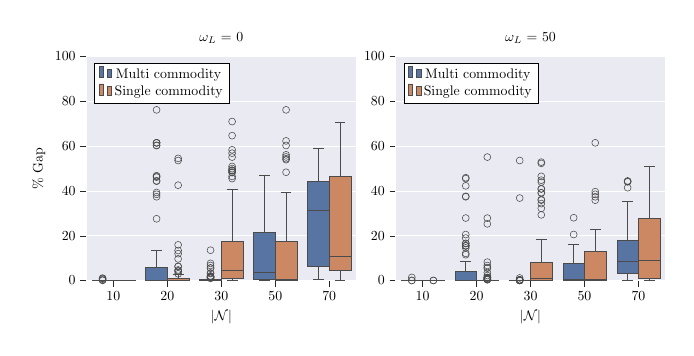
\begin{tikzpicture}[scale=0.5]

        \definecolor{darkslategray38}{RGB}{38,38,38}
        \definecolor{darkslategray75}{RGB}{75,75,75}
        \definecolor{lavender234234242}{RGB}{234,234,242}
        \definecolor{peru20313699}{RGB}{203,136,99}
        \definecolor{steelblue88116163}{RGB}{88,116,163}
        
        \begin{groupplot}[group style={group size=2 by 1}]
        \nextgroupplot[
            axis background/.style={fill=color0},
            axis line style={white},
            tick align=outside,
            title={$\omega_L$ = 0},
            x grid style={white},
            xtick pos = left,
            ytick pos = left,
            xlabel={$|\mathcal N|$},
            % xmajorticks=false,
            xmin=-0.5, xmax=4.5,
            xtick style={color=white!15!black},
            xtick={0,1,2,3,4},
            xticklabels={10, 20, 30, 50, 70},
            y grid style={white},
            ylabel={\% Gap},
            ymajorgrids,
            % ymajorticks=false,
            ymin=-0.05, ymax= 100,
            ytick style={color=white!15!black},
            %ytick={-0.2,0,0.2,0.4,0.6,0.8,1,1.2},
            %yticklabels={−0.2,0.0,0.2,0.4,0.6,0.8,1.0,1.2},
            legend pos = north west
        ]
        \addlegendimage{ybar,ybar legend,draw=white!29.8039215686275!black,fill=color1,line width=0.3pt}
        \addlegendimage{ybar,ybar legend,draw=white!29.8039215686275!black,fill=color2,line width=0.3pt}
        \addlegendentry{Multi commodity}
        \addlegendentry{Single commodity}

        \path [draw=darkslategray75, fill=steelblue88116163]
        (axis cs:-0.4,0.000293002358275815)
        --(axis cs:0,0.000293002358275815)
        --(axis cs:0,0.00784452228026413)
        --(axis cs:-0.4,0.00784452228026413)
        --(axis cs:-0.4,0.000293002358275815)
        --cycle;
        \addplot [darkslategray75]
        table {%
        -0.2 0.000293002358275815
        -0.2 0
        };
        \addplot [darkslategray75]
        table {%
        -0.2 0.00784452228026413
        -0.2 0.01505238246347
        };
        \addplot [darkslategray75]
        table {%
        -0.3 0
        -0.1 0
        };
        \addplot [darkslategray75]
        table {%
        -0.3 0.01505238246347
        -0.1 0.01505238246347
        };
        \addplot [black, mark=o, mark size=2.5, mark options={solid,fill opacity=0,draw=darkslategray75}, only marks]
        table {%
        -0.2 0.58100173524854
        -0.2 0.91372211674591
        -0.2 0.09269252954582
        -0.2 0.14930669918111
        -0.2 1.05559728934607
        };
        \path [draw=darkslategray75, fill=steelblue88116163]
        (axis cs:0.6,0.00484933953710631)
        --(axis cs:1,0.00484933953710631)
        --(axis cs:1,5.75755760972038)
        --(axis cs:0.6,5.75755760972038)
        --(axis cs:0.6,0.00484933953710631)
        --cycle;
        \addplot [darkslategray75]
        table {%
        0.8 0.00484933953710631
        0.8 0
        };
        \addplot [darkslategray75]
        table {%
        0.8 5.75755760972038
        0.8 13.7122896462636
        };
        \addplot [darkslategray75]
        table {%
        0.7 0
        0.9 0
        };
        \addplot [darkslategray75]
        table {%
        0.7 13.7122896462636
        0.9 13.7122896462636
        };
        \addplot [black, mark=o, mark size=2.5, mark options={solid,fill opacity=0,draw=darkslategray75}, only marks]
        table {%
        0.8 44.5278992166011
        0.8 60.2102555962561
        0.8 61.4574898485696
        0.8 38.4803173503948
        0.8 46.779422109651
        0.8 76.1664598753247
        0.8 61.4574898485696
        0.8 27.5604455287091
        0.8 46.1343655535057
        0.8 60.3471795459629
        0.8 39.3038282261008
        0.8 61.4574898485696
        0.8 37.3850550553553
        0.8 46.4726564313443
        0.8 44.3304667808476
        };
        \path [draw=darkslategray75, fill=steelblue88116163]
        (axis cs:1.6,0.000360423742480359)
        --(axis cs:2,0.000360423742480359)
        --(axis cs:2,0.335829218102795)
        --(axis cs:1.6,0.335829218102795)
        --(axis cs:1.6,0.000360423742480359)
        --cycle;
        \addplot [darkslategray75]
        table {%
        1.8 0.000360423742480359
        1.8 0
        };
        \addplot [darkslategray75]
        table {%
        1.8 0.335829218102795
        1.8 0.7092072471079
        };
        \addplot [darkslategray75]
        table {%
        1.7 0
        1.9 0
        };
        \addplot [darkslategray75]
        table {%
        1.7 0.7092072471079
        1.9 0.7092072471079
        };
        \addplot [black, mark=o, mark size=2.5, mark options={solid,fill opacity=0,draw=darkslategray75}, only marks]
        table {%
        1.8 0.95183679858894
        1.8 1.90534300789556
        1.8 5.50118923455796
        1.8 5.64452209279346
        1.8 1.53906513721942
        1.8 3.12081731261197
        1.8 1.51143637218262
        1.8 13.5254016361461
        1.8 3.36369177194993
        1.8 1.56430521697211
        1.8 6.70614284710501
        1.8 7.65898287087026
        1.8 1.25531680705684
        1.8 2.02327688549173
        1.8 1.28736985216044
        };
        \path [draw=darkslategray75, fill=steelblue88116163]
        (axis cs:2.6,0.34963035249505)
        --(axis cs:3,0.34963035249505)
        --(axis cs:3,21.3123544993094)
        --(axis cs:2.6,21.3123544993094)
        --(axis cs:2.6,0.34963035249505)
        --cycle;
        \addplot [darkslategray75]
        table {%
        2.8 0.34963035249505
        2.8 0.000741544897730709
        };
        \addplot [darkslategray75]
        table {%
        2.8 21.3123544993094
        2.8 46.9113227056868
        };
        \addplot [darkslategray75]
        table {%
        2.7 0.000741544897730709
        2.9 0.000741544897730709
        };
        \addplot [darkslategray75]
        table {%
        2.7 46.9113227056868
        2.9 46.9113227056868
        };
        \path [draw=darkslategray75, fill=steelblue88116163]
        (axis cs:3.6,6.42032337800469)
        --(axis cs:4,6.42032337800469)
        --(axis cs:4,44.3503805391937)
        --(axis cs:3.6,44.3503805391937)
        --(axis cs:3.6,6.42032337800469)
        --cycle;
        \addplot [darkslategray75]
        table {%
        3.8 6.42032337800469
        3.8 0.5662211319471
        };
        \addplot [darkslategray75]
        table {%
        3.8 44.3503805391937
        3.8 58.9152830341672
        };
        \addplot [darkslategray75]
        table {%
        3.7 0.5662211319471
        3.9 0.5662211319471
        };
        \addplot [darkslategray75]
        table {%
        3.7 58.9152830341672
        3.9 58.9152830341672
        };
        \path [draw=darkslategray75, fill=peru20313699]
        (axis cs:5.55111512312578e-17,9.60228596151803e-05)
        --(axis cs:0.4,9.60228596151803e-05)
        --(axis cs:0.4,0.006601368171869)
        --(axis cs:5.55111512312578e-17,0.006601368171869)
        --(axis cs:5.55111512312578e-17,9.60228596151803e-05)
        --cycle;
        \addplot [darkslategray75]
        table {%
        0.2 9.60228596151803e-05
        0.2 0
        };
        \addplot [darkslategray75]
        table {%
        0.2 0.006601368171869
        0.2 0.00977473330891838
        };
        \addplot [darkslategray75]
        table {%
        0.1 0
        0.3 0
        };
        \addplot [darkslategray75]
        table {%
        0.1 0.00977473330891838
        0.3 0.00977473330891838
        };
        \path [draw=darkslategray75, fill=peru20313699]
        (axis cs:1,0.00490420577831317)
        --(axis cs:1.4,0.00490420577831317)
        --(axis cs:1.4,1.16155330202884)
        --(axis cs:1,1.16155330202884)
        --(axis cs:1,0.00490420577831317)
        --cycle;
        \addplot [darkslategray75]
        table {%
        1.2 0.00490420577831317
        1.2 2.65150553742482e-05
        };
        \addplot [darkslategray75]
        table {%
        1.2 1.16155330202884
        1.2 2.83889869055089
        };
        \addplot [darkslategray75]
        table {%
        1.1 2.65150553742482e-05
        1.3 2.65150553742482e-05
        };
        \addplot [darkslategray75]
        table {%
        1.1 2.83889869055089
        1.3 2.83889869055089
        };
        \addplot [black, mark=o, mark size=2.5, mark options={solid,fill opacity=0,draw=darkslategray75}, only marks]
        table {%
        1.2 11.9890325401032
        1.2 9.65754332185507
        1.2 6.34814232844278
        1.2 6.21312321689917
        1.2 15.9186172784106
        1.2 4.71203324430282
        1.2 42.5477051126761
        1.2 4.10294448576652
        1.2 2.97995329446986
        1.2 54.5096062256846
        1.2 53.5660174944889
        1.2 4.30846890205483
        1.2 13.3939724248486
        };
        \path [draw=darkslategray75, fill=peru20313699]
        (axis cs:2,1.02885889281845)
        --(axis cs:2.4,1.02885889281845)
        --(axis cs:2.4,17.3591362396042)
        --(axis cs:2,17.3591362396042)
        --(axis cs:2,1.02885889281845)
        --cycle;
        \addplot [darkslategray75]
        table {%
        2.2 1.02885889281845
        2.2 1.73791944892168e-05
        };
        \addplot [darkslategray75]
        table {%
        2.2 17.3591362396042
        2.2 40.9101694279538
        };
        \addplot [darkslategray75]
        table {%
        2.1 1.73791944892168e-05
        2.3 1.73791944892168e-05
        };
        \addplot [darkslategray75]
        table {%
        2.1 40.9101694279538
        2.3 40.9101694279538
        };
        \addplot [black, mark=o, mark size=2.5, mark options={solid,fill opacity=0,draw=darkslategray75}, only marks]
        table {%
        2.2 48.1638666304086
        2.2 70.9594307239694
        2.2 50.9197782515743
        2.2 49.9773745620345
        2.2 49.0465971691944
        2.2 64.6743696766902
        2.2 45.4967265996127
        2.2 58.3387306181939
        2.2 49.2361738570426
        2.2 49.0465971691944
        2.2 56.8301459407719
        2.2 55.0909518040008
        2.2 46.4652765282972
        2.2 48.4077331573171
        };
        \path [draw=darkslategray75, fill=peru20313699]
        (axis cs:3,0.00550107047973292)
        --(axis cs:3.4,0.00550107047973292)
        --(axis cs:3.4,17.4915657228882)
        --(axis cs:3,17.4915657228882)
        --(axis cs:3,0.00550107047973292)
        --cycle;
        \addplot [darkslategray75]
        table {%
        3.2 0.00550107047973292
        3.2 6.37774837364641e-05
        };
        \addplot [darkslategray75]
        table {%
        3.2 17.4915657228882
        3.2 39.1920303109229
        };
        \addplot [darkslategray75]
        table {%
        3.1 6.37774837364641e-05
        3.3 6.37774837364641e-05
        };
        \addplot [darkslategray75]
        table {%
        3.1 39.1920303109229
        3.3 39.1920303109229
        };
        \addplot [black, mark=o, mark size=2.5, mark options={solid,fill opacity=0,draw=darkslategray75}, only marks]
        table {%
        3.2 60.2709633434356
        3.2 55.1585827041495
        3.2 56.0857661446653
        3.2 76.1664598753247
        3.2 53.9277771386916
        3.2 48.3249398291429
        3.2 62.325384033416
        3.2 54.3645110945196
        };
        \path [draw=darkslategray75, fill=peru20313699]
        (axis cs:4,4.38234922719548)
        --(axis cs:4.4,4.38234922719548)
        --(axis cs:4.4,46.5229083039696)
        --(axis cs:4,46.5229083039696)
        --(axis cs:4,4.38234922719548)
        --cycle;
        \addplot [darkslategray75]
        table {%
        4.2 4.38234922719548
        4.2 0.311196843358
        };
        \addplot [darkslategray75]
        table {%
        4.2 46.5229083039696
        4.2 70.7663547771197
        };
        \addplot [darkslategray75]
        table {%
        4.1 0.311196843358
        4.3 0.311196843358
        };
        \addplot [darkslategray75]
        table {%
        4.1 70.7663547771197
        4.3 70.7663547771197
        };
        \addplot [darkslategray75]
        table {%
        -0.4 0.00303395684377409
        0 0.00303395684377409
        };
        \addplot [darkslategray75]
        table {%
        0.6 0.06586689085259
        1 0.06586689085259
        };
        \addplot [darkslategray75]
        table {%
        1.6 0.00411323950857388
        2 0.00411323950857388
        };
        \addplot [darkslategray75]
        table {%
        2.6 3.56307573655619
        3 3.56307573655619
        };
        \addplot [darkslategray75]
        table {%
        3.6 31.555460121186
        4 31.555460121186
        };
        \addplot [darkslategray75]
        table {%
        5.55111512312578e-17 0.00181700814919011
        0.4 0.00181700814919011
        };
        \addplot [darkslategray75]
        table {%
        1 0.11138150680879
        1.4 0.11138150680879
        };
        \addplot [darkslategray75]
        table {%
        2 4.37196011888598
        2.4 4.37196011888598
        };
        \addplot [darkslategray75]
        table {%
        3 0.74873802568304
        3.4 0.74873802568304
        };
        \addplot [darkslategray75]
        table {%
        4 10.6250462617547
        4.4 10.6250462617547
        };
        
        \nextgroupplot[
			axis background/.style={fill=color0},
			axis line style={white},
			tick align=outside,
			title={$\omega_L$ = 50},
			x grid style={white},
			xtick pos = left,
			ytick pos = left,
			xlabel={$|\mathcal N|$},
			% xmajorticks=false,
			xmin=-0.5, xmax=4.5,
			xtick style={color=white!15!black},
			xtick={0,1,2,3,4},
			xticklabels={10, 20, 30, 50, 70},
			y grid style={white},
			% ylabel={\% Gap},
			ymajorgrids,
			% ymajorticks=false,
			ymin=-0.05, ymax= 100,
			ytick style={color=white!15!black},
			%ytick={-0.2,0,0.2,0.4,0.6,0.8,1,1.2},
			%yticklabels={−0.2,0.0,0.2,0.4,0.6,0.8,1.0,1.2},
			legend pos = north west
			]
			\addlegendimage{ybar,ybar legend,draw=white!29.8039215686275!black,fill=color1,line width=0.3pt}
			\addlegendimage{ybar,ybar legend,draw=white!29.8039215686275!black,fill=color2,line width=0.3pt}
			\addlegendentry{Multi commodity}
			\addlegendentry{Single commodity}
        
        \path [draw=darkslategray75, fill=steelblue88116163]
        (axis cs:-0.4,0.000515183242195497)
        --(axis cs:0,0.000515183242195497)
        --(axis cs:0,0.00687490024650642)
        --(axis cs:-0.4,0.00687490024650642)
        --(axis cs:-0.4,0.000515183242195497)
        --cycle;
        \addplot [darkslategray75]
        table {%
        -0.2 0.000515183242195497
        -0.2 0
        };
        \addplot [darkslategray75]
        table {%
        -0.2 0.00687490024650642
        -0.2 0.01413024739351
        };
        \addplot [darkslategray75]
        table {%
        -0.3 0
        -0.1 0
        };
        \addplot [darkslategray75]
        table {%
        -0.3 0.01413024739351
        -0.1 0.01413024739351
        };
        \addplot [black, mark=o, mark size=2.5, mark options={solid,fill opacity=0,draw=darkslategray75}, only marks]
        table {%
        -0.2 1.37050415595726
        -0.2 0.01703082689314
        -0.2 0.0199753180264
        };
        \path [draw=darkslategray75, fill=steelblue88116163]
        (axis cs:0.6,0.00155583955716873)
        --(axis cs:1,0.00155583955716873)
        --(axis cs:1,4.32742467186743)
        --(axis cs:0.6,4.32742467186743)
        --(axis cs:0.6,0.00155583955716873)
        --cycle;
        \addplot [darkslategray75]
        table {%
        0.8 0.00155583955716873
        0.8 0
        };
        \addplot [darkslategray75]
        table {%
        0.8 4.32742467186743
        0.8 8.69366739960474
        };
        \addplot [darkslategray75]
        table {%
        0.7 0
        0.9 0
        };
        \addplot [darkslategray75]
        table {%
        0.7 8.69366739960474
        0.9 8.69366739960474
        };
        \addplot [black, mark=o, mark size=2.5, mark options={solid,fill opacity=0,draw=darkslategray75}, only marks]
        table {%
        0.8 16.5144185918996
        0.8 37.58225787848
        0.8 16.5850478702956
        0.8 45.8798530445469
        0.8 20.5187883469259
        0.8 42.2600060466592
        0.8 14.5639104056618
        0.8 37.375563490165
        0.8 18.9516447610634
        0.8 15.4998425435517
        0.8 45.4824508034552
        0.8 15.5391644987807
        0.8 27.8843164530688
        0.8 12.1129478137183
        0.8 11.5101676563094
        0.8 15.4637599715583
        };
        \path [draw=darkslategray75, fill=steelblue88116163]
        (axis cs:1.6,0.000360352716531846)
        --(axis cs:2,0.000360352716531846)
        --(axis cs:2,0.01493625151112)
        --(axis cs:1.6,0.01493625151112)
        --(axis cs:1.6,0.000360352716531846)
        --cycle;
        \addplot [darkslategray75]
        table {%
        1.8 0.000360352716531846
        1.8 0
        };
        \addplot [darkslategray75]
        table {%
        1.8 0.01493625151112
        1.8 0.03298707850995
        };
        \addplot [darkslategray75]
        table {%
        1.7 0
        1.9 0
        };
        \addplot [darkslategray75]
        table {%
        1.7 0.03298707850995
        1.9 0.03298707850995
        };
        \addplot [black, mark=o, mark size=2.5, mark options={solid,fill opacity=0,draw=darkslategray75}, only marks]
        table {%
        1.8 0.09577552511881
        1.8 0.20388751995576
        1.8 1.14793439732296
        1.8 0.18772503679995
        1.8 36.8059943370725
        1.8 0.14231902035742
        1.8 0.06001847168773
        1.8 0.04135087863621
        1.8 53.5661945854495
        1.8 0.27211674738245
        1.8 0.04917247892112
        1.8 0.32664878401191
        1.8 0.05477244326215
        1.8 0.20965852512651
        1.8 0.11271745269773
        };
        \path [draw=darkslategray75, fill=steelblue88116163]
        (axis cs:2.6,0.0574263596422475)
        --(axis cs:3,0.0574263596422475)
        --(axis cs:3,7.50779151692795)
        --(axis cs:2.6,7.50779151692795)
        --(axis cs:2.6,0.0574263596422475)
        --cycle;
        \addplot [darkslategray75]
        table {%
        2.8 0.0574263596422475
        2.8 1.23694643955478e-08
        };
        \addplot [darkslategray75]
        table {%
        2.8 7.50779151692795
        2.8 16.1485551799772
        };
        \addplot [darkslategray75]
        table {%
        2.7 1.23694643955478e-08
        2.9 1.23694643955478e-08
        };
        \addplot [darkslategray75]
        table {%
        2.7 16.1485551799772
        2.9 16.1485551799772
        };
        \addplot [black, mark=o, mark size=2.5, mark options={solid,fill opacity=0,draw=darkslategray75}, only marks]
        table {%
        2.8 28.0140586931555
        2.8 20.5391426581447
        };
        \path [draw=darkslategray75, fill=steelblue88116163]
        (axis cs:3.6,3.12299867330611)
        --(axis cs:4,3.12299867330611)
        --(axis cs:4,18.1298194801598)
        --(axis cs:3.6,18.1298194801598)
        --(axis cs:3.6,3.12299867330611)
        --cycle;
        \addplot [darkslategray75]
        table {%
        3.8 3.12299867330611
        3.8 0.00871839567541549
        };
        \addplot [darkslategray75]
        table {%
        3.8 18.1298194801598
        3.8 35.1714108725056
        };
        \addplot [darkslategray75]
        table {%
        3.7 0.00871839567541549
        3.9 0.00871839567541549
        };
        \addplot [darkslategray75]
        table {%
        3.7 35.1714108725056
        3.9 35.1714108725056
        };
        \addplot [black, mark=o, mark size=2.5, mark options={solid,fill opacity=0,draw=darkslategray75}, only marks]
        table {%
        3.8 44.0581141231469
        3.8 44.4423266599724
        3.8 41.4203741441358
        3.8 44.2170793557533
        };
        \path [draw=darkslategray75, fill=peru20313699]
        (axis cs:5.55111512312578e-17,0.000184736299961658)
        --(axis cs:0.4,0.000184736299961658)
        --(axis cs:0.4,0.00581738018233628)
        --(axis cs:5.55111512312578e-17,0.00581738018233628)
        --(axis cs:5.55111512312578e-17,0.000184736299961658)
        --cycle;
        \addplot [darkslategray75]
        table {%
        0.2 0.000184736299961658
        0.2 0
        };
        \addplot [darkslategray75]
        table {%
        0.2 0.00581738018233628
        0.2 0.00977473330891838
        };
        \addplot [darkslategray75]
        table {%
        0.1 0
        0.3 0
        };
        \addplot [darkslategray75]
        table {%
        0.1 0.00977473330891838
        0.3 0.00977473330891838
        };
        \addplot [black, mark=o, mark size=2.5, mark options={solid,fill opacity=0,draw=darkslategray75}, only marks]
        table {%
        0.2 0.01716686330995
        0.2 0.01647584015881
        };
        \path [draw=darkslategray75, fill=peru20313699]
        (axis cs:1,0.00138562313667153)
        --(axis cs:1.4,0.00138562313667153)
        --(axis cs:1.4,0.127417112286995)
        --(axis cs:1,0.127417112286995)
        --(axis cs:1,0.00138562313667153)
        --cycle;
        \addplot [darkslategray75]
        table {%
        1.2 0.00138562313667153
        1.2 1.23238990202196e-06
        };
        \addplot [darkslategray75]
        table {%
        1.2 0.127417112286995
        1.2 0.29352631475098
        };
        \addplot [darkslategray75]
        table {%
        1.1 1.23238990202196e-06
        1.3 1.23238990202196e-06
        };
        \addplot [darkslategray75]
        table {%
        1.1 0.29352631475098
        1.3 0.29352631475098
        };
        \addplot [black, mark=o, mark size=2.5, mark options={solid,fill opacity=0,draw=darkslategray75}, only marks]
        table {%
        1.2 1.22352466178519
        1.2 0.43882455878509
        1.2 0.33564677662856
        1.2 0.70966022681049
        1.2 55.0927304097178
        1.2 2.22699430432005
        1.2 3.55634951427686
        1.2 27.8573969203345
        1.2 0.50761851152641
        1.2 1.14504436032003
        1.2 5.50118923455796
        1.2 5.78034398464468
        1.2 1.3578970950807
        1.2 1.24435283038106
        1.2 0.59456366499597
        1.2 25.2965408171533
        1.2 8.18903993807602
        1.2 6.70614284710501
        1.2 1.25665177062541
        1.2 1.25983011206012
        };
        \path [draw=darkslategray75, fill=peru20313699]
        (axis cs:2,0.0132935463308)
        --(axis cs:2.4,0.0132935463308)
        --(axis cs:2.4,8.30152980907663)
        --(axis cs:2,8.30152980907663)
        --(axis cs:2,0.0132935463308)
        --cycle;
        \addplot [darkslategray75]
        table {%
        2.2 0.0132935463308
        2.2 1.67557903244621e-05
        };
        \addplot [darkslategray75]
        table {%
        2.2 8.30152980907663
        2.2 18.6131405275723
        };
        \addplot [darkslategray75]
        table {%
        2.1 1.67557903244621e-05
        2.3 1.67557903244621e-05
        };
        \addplot [darkslategray75]
        table {%
        2.1 18.6131405275723
        2.3 18.6131405275723
        };
        \addplot [black, mark=o, mark size=2.5, mark options={solid,fill opacity=0,draw=darkslategray75}, only marks]
        table {%
        2.2 52.2832988646815
        2.2 39.1426101854291
        2.2 46.4974771658672
        2.2 32.2114077330974
        2.2 40.9708760613519
        2.2 40.8360455396458
        2.2 43.9556023324077
        2.2 34.3402598231523
        2.2 29.3165356078277
        2.2 35.8462454472341
        2.2 39.1426101854291
        2.2 44.7781213785001
        2.2 36.1317828429306
        2.2 52.843610049725
        };
        \path [draw=darkslategray75, fill=peru20313699]
        (axis cs:3,0.00723658933683095)
        --(axis cs:3.4,0.00723658933683095)
        --(axis cs:3.4,13.1024043379052)
        --(axis cs:3,13.1024043379052)
        --(axis cs:3,0.00723658933683095)
        --cycle;
        \addplot [darkslategray75]
        table {%
        3.2 0.00723658933683095
        3.2 8.5770369418658e-06
        };
        \addplot [darkslategray75]
        table {%
        3.2 13.1024043379052
        3.2 22.9318519745265
        };
        \addplot [darkslategray75]
        table {%
        3.1 8.5770369418658e-06
        3.3 8.5770369418658e-06
        };
        \addplot [darkslategray75]
        table {%
        3.1 22.9318519745265
        3.3 22.9318519745265
        };
        \addplot [black, mark=o, mark size=2.5, mark options={solid,fill opacity=0,draw=darkslategray75}, only marks]
        table {%
        3.2 38.4803221467685
        3.2 39.6524849935639
        3.2 61.4574898485696
        3.2 35.8439835135959
        3.2 37.3850550553553
        };
        \path [draw=darkslategray75, fill=peru20313699]
        (axis cs:4,1.07525124139856)
        --(axis cs:4.4,1.07525124139856)
        --(axis cs:4.4,27.9753951813516)
        --(axis cs:4,27.9753951813516)
        --(axis cs:4,1.07525124139856)
        --cycle;
        \addplot [darkslategray75]
        table {%
        4.2 1.07525124139856
        4.2 0.16857617863507
        };
        \addplot [darkslategray75]
        table {%
        4.2 27.9753951813516
        4.2 50.9197782515743
        };
        \addplot [darkslategray75]
        table {%
        4.1 0.16857617863507
        4.3 0.16857617863507
        };
        \addplot [darkslategray75]
        table {%
        4.1 50.9197782515743
        4.3 50.9197782515743
        };
        \addplot [darkslategray75]
        table {%
        -0.4 0.00461948907707796
        0 0.00461948907707796
        };
        \addplot [darkslategray75]
        table {%
        0.6 0.00932646642780936
        1 0.00932646642780936
        };
        \addplot [darkslategray75]
        table {%
        1.6 0.00411323950857388
        2 0.00411323950857388
        };
        \addplot [darkslategray75]
        table {%
        2.6 0.534365257682265
        3 0.534365257682265
        };
        \addplot [darkslategray75]
        table {%
        3.6 8.68069027068688
        4 8.68069027068688
        };
        \addplot [darkslategray75]
        table {%
        5.55111512312578e-17 0.00208347761421592
        0.4 0.00208347761421592
        };
        \addplot [darkslategray75]
        table {%
        1 0.00768661896472272
        1.4 0.00768661896472272
        };
        \addplot [darkslategray75]
        table {%
        2 1.14632265303888
        2.4 1.14632265303888
        };
        \addplot [darkslategray75]
        table {%
        3 0.657776802322915
        3.4 0.657776802322915
        };
        \addplot [darkslategray75]
        table {%
        4 8.999049527781
        4.4 8.999049527781
        };
        \end{groupplot}
        
        \end{tikzpicture}
        
\end{figure}

			\label{fig:results_wL}
			% This file was created with tikzplotlib v0.10.1.
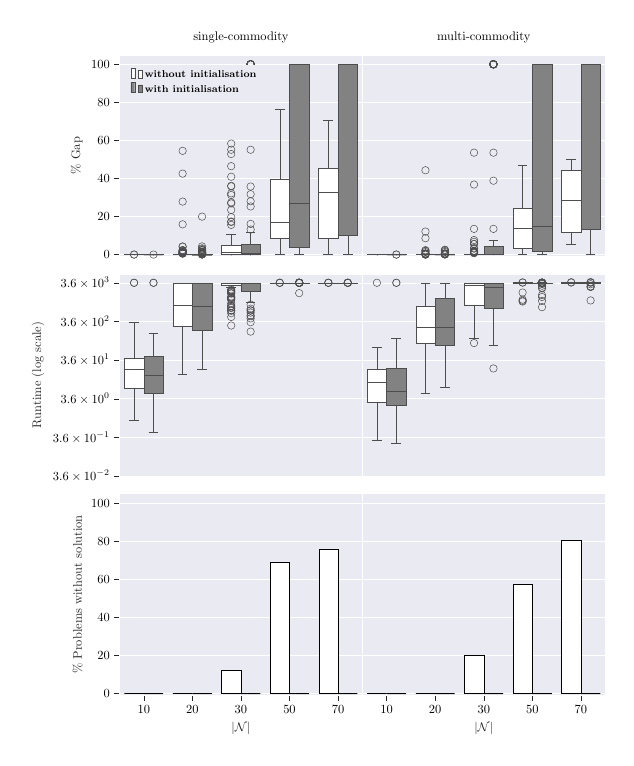
\begin{tikzpicture}[scale=0.45]

\definecolor{darkslategray38}{RGB}{38,38,38}
\definecolor{darkslategray66}{RGB}{66,66,66}
\definecolor{darkslategray77}{RGB}{77,77,77}
\definecolor{gray130}{RGB}{130,130,130}
\definecolor{lavender234234242}{RGB}{234,234,242}

\begin{groupplot}[group style={group size=2 by 3, vertical sep=0.5cm, horizontal sep=0pt}]
\nextgroupplot[
axis background/.style={fill=lavender234234242},
axis line style={white},
legend cell align={left},
legend style={
  fill opacity=1,
  draw opacity=1,
  text opacity=1,
  font=\footnotesize,
  at={(0.03,0.95)},
  anchor=north west,
  draw=none,
  fill=lavender234234242
},
scaled x ticks=manual:{}{\pgfmathparse{#1}},
tick align=outside,
title={single-commodity},
x grid style={white},
xmajorticks=false,
xmin=-0.5, xmax=4.5,
xtick style={color=darkslategray38},
xticklabels={},
y grid style={white},
ylabel=\textcolor{darkslategray38}{\% Gap},
ymajorgrids,
ymin=-1, ymax=105,
ytick style={color=darkslategray38},
ytick={0,20,40,60,80,100},
yticklabels={
  \(\displaystyle {0}\),
  \(\displaystyle {20}\),
  \(\displaystyle {40}\),
  \(\displaystyle {60}\),
  \(\displaystyle {80}\),
  \(\displaystyle {100}\)
}
]
\addlegendimage{ybar,ybar legend,draw=white!29.8039215686275!black,fill=white,line width=0.3pt}
\addlegendimage{ybar,ybar legend,draw=white!29.8039215686275!black,fill=gray130,line width=0.3pt}
\addlegendentry{\textbf{without initialisation}}
\addlegendentry{\textbf{with initialisation}}
\path [draw=darkslategray77, fill=white]
(axis cs:-0.4,0.00011478159972593)
--(axis cs:0,0.00011478159972593)
--(axis cs:0,0.00532018841657887)
--(axis cs:-0.4,0.00532018841657887)
--(axis cs:-0.4,0.00011478159972593)
--cycle;
\addplot [darkslategray77, forget plot]
table {%
-0.2 0.00011478159972593
-0.2 0
};
\addplot [darkslategray77, forget plot]
table {%
-0.2 0.00532018841657887
-0.2 0.0097037454459847
};
\addplot [darkslategray77, forget plot]
table {%
-0.3 0
-0.1 0
};
\addplot [darkslategray77, forget plot]
table {%
-0.3 0.0097037454459847
-0.1 0.0097037454459847
};
\addplot [black, mark=o, mark size=3, mark options={solid,fill opacity=0,draw=darkslategray77}, only marks, forget plot]
table {%
-0.2 0.01716686330995
-0.2 0.01647584015881
};
\path [draw=darkslategray77, fill=white]
(axis cs:0.6,0.00123593887583794)
--(axis cs:1,0.00123593887583794)
--(axis cs:1,0.176609003171867)
--(axis cs:0.6,0.176609003171867)
--(axis cs:0.6,0.00123593887583794)
--cycle;
\addplot [darkslategray77, forget plot]
table {%
0.8 0.00123593887583794
0.8 1.23238990202196e-06
};
\addplot [darkslategray77, forget plot]
table {%
0.8 0.176609003171867
0.8 0.38095591660376
};
\addplot [darkslategray77, forget plot]
table {%
0.7 1.23238990202196e-06
0.9 1.23238990202196e-06
};
\addplot [darkslategray77, forget plot]
table {%
0.7 0.38095591660376
0.9 0.38095591660376
};
\addplot [black, mark=o, mark size=3, mark options={solid,fill opacity=0,draw=darkslategray77}, only marks, forget plot]
table {%
0.8 0.75102225362427
0.8 0.74533367953655
0.8 1.90909217578163
0.8 15.9186172784106
0.8 2.3717273331677
0.8 2.22699430432005
0.8 27.8573969203345
0.8 0.50761851152641
0.8 42.5477051126761
0.8 4.10294448576652
0.8 1.3578970950807
0.8 1.24435283038106
0.8 54.5096062256846
0.8 1.39481407853686
0.8 0.91208432423258
0.8 4.30846890205483
0.8 1.63478411512995
0.8 0.74929264773176
0.8 0.77460278533438
0.8 0.75113280024235
0.8 0.56346975769638
0.8 1.29534349751957
0.8 1.06770605686595
0.8 2.26902786496918
};
\path [draw=darkslategray77, fill=white]
(axis cs:1.6,0.00994756655080013)
--(axis cs:2,0.00994756655080013)
--(axis cs:2,5.11996796876474)
--(axis cs:1.6,5.11996796876474)
--(axis cs:1.6,0.00994756655080013)
--cycle;
\addplot [darkslategray77, forget plot]
table {%
1.8 0.00994756655080013
1.8 1.67557903244621e-05
};
\addplot [darkslategray77, forget plot]
table {%
1.8 5.11996796876474
1.8 10.7563760399151
};
\addplot [darkslategray77, forget plot]
table {%
1.7 1.67557903244621e-05
1.9 1.67557903244621e-05
};
\addplot [darkslategray77, forget plot]
table {%
1.7 10.7563760399151
1.9 10.7563760399151
};
\addplot [black, mark=o, mark size=3, mark options={solid,fill opacity=0,draw=darkslategray77}, only marks, forget plot]
table {%
1.8 31.29987005106
1.8 23.4357479559391
1.8 15.6159206199839
1.8 17.1402788560426
1.8 32.2114077330974
1.8 58.3387306181939
1.8 55.0909518040008
1.8 35.8462454472341
1.8 46.4652765282972
1.8 40.9101694279538
1.8 26.8810865527709
1.8 17.3591362396042
1.8 36.1317828429306
1.8 27.4529522129236
1.8 19.7119665130021
1.8 52.843610049725
};
\path [draw=darkslategray77, fill=white]
(axis cs:2.6,8.75016870597507)
--(axis cs:3,8.75016870597507)
--(axis cs:3,39.6524849935639)
--(axis cs:2.6,39.6524849935639)
--(axis cs:2.6,8.75016870597507)
--cycle;
\addplot [darkslategray77, forget plot]
table {%
2.8 8.75016870597507
2.8 0.31119684335765
};
\addplot [darkslategray77, forget plot]
table {%
2.8 39.6524849935639
2.8 76.1664598753247
};
\addplot [darkslategray77, forget plot]
table {%
2.7 0.31119684335765
2.9 0.31119684335765
};
\addplot [darkslategray77, forget plot]
table {%
2.7 76.1664598753247
2.9 76.1664598753247
};
\path [draw=darkslategray77, fill=white]
(axis cs:3.6,8.5386498315641)
--(axis cs:4,8.5386498315641)
--(axis cs:4,45.4947670329185)
--(axis cs:3.6,45.4947670329185)
--(axis cs:3.6,8.5386498315641)
--cycle;
\addplot [darkslategray77, forget plot]
table {%
3.8 8.5386498315641
3.8 0.43407388878438
};
\addplot [darkslategray77, forget plot]
table {%
3.8 45.4947670329185
3.8 70.7663547771197
};
\addplot [darkslategray77, forget plot]
table {%
3.7 0.43407388878438
3.9 0.43407388878438
};
\addplot [darkslategray77, forget plot]
table {%
3.7 70.7663547771197
3.9 70.7663547771197
};
\path [draw=darkslategray77, fill=gray130]
(axis cs:5.55111512312578e-17,0.000125310856254314)
--(axis cs:0.4,0.000125310856254314)
--(axis cs:0.4,0.00697308280707184)
--(axis cs:5.55111512312578e-17,0.00697308280707184)
--(axis cs:5.55111512312578e-17,0.000125310856254314)
--cycle;
\addplot [darkslategray77, forget plot]
table {%
0.2 0.000125310856254314
0.2 0
};
\addplot [darkslategray77, forget plot]
table {%
0.2 0.00697308280707184
0.2 0.01647584015881
};
\addplot [darkslategray77, forget plot]
table {%
0.1 0
0.3 0
};
\addplot [darkslategray77, forget plot]
table {%
0.1 0.01647584015881
0.3 0.01647584015881
};
\addplot [black, mark=o, mark size=3, mark options={solid,fill opacity=0,draw=darkslategray77}, only marks, forget plot]
table {%
0.2 0.02011441348994
};
\path [draw=darkslategray77, fill=gray130]
(axis cs:1,0.000821220506492723)
--(axis cs:1.4,0.000821220506492723)
--(axis cs:1.4,0.0175696673882075)
--(axis cs:1,0.0175696673882075)
--(axis cs:1,0.000821220506492723)
--cycle;
\addplot [darkslategray77, forget plot]
table {%
1.2 0.000821220506492723
1.2 0
};
\addplot [darkslategray77, forget plot]
table {%
1.2 0.0175696673882075
1.2 0.02685279569932
};
\addplot [darkslategray77, forget plot]
table {%
1.1 0
1.3 0
};
\addplot [darkslategray77, forget plot]
table {%
1.1 0.02685279569932
1.3 0.02685279569932
};
\addplot [black, mark=o, mark size=3, mark options={solid,fill opacity=0,draw=darkslategray77}, only marks, forget plot]
table {%
1.2 2.83799665004793
1.2 0.58100173524854
1.2 1.6171585193978
1.2 2.39411320354555
1.2 2.37164865736079
1.2 0.71879150656757
1.2 0.50551113375136
1.2 19.9498585235363
1.2 3.3082368144088
1.2 1.3578970950807
1.2 1.39920921995736
1.2 1.39540800235063
1.2 0.91372211674591
1.2 0.09269252954582
1.2 4.30277114543275
1.2 1.37050415595726
1.2 0.06398391308567
1.2 0.74888508448456
1.2 0.50642041837589
1.2 0.74873802568304
1.2 0.13279523160694
1.2 0.20951223165075
1.2 0.56513013609238
1.2 1.00407859807943
1.2 0.29641506935428
1.2 1.06775126312851
1.2 1.05559728934607
1.2 2.26967819952955
};
\path [draw=darkslategray77, fill=gray130]
(axis cs:2,0.00900664922130094)
--(axis cs:2.4,0.00900664922130094)
--(axis cs:2.4,5.25234785804683)
--(axis cs:2,5.25234785804683)
--(axis cs:2,0.00900664922130094)
--cycle;
\addplot [darkslategray77, forget plot]
table {%
2.2 0.00900664922130094
2.2 4.941058745378e-05
};
\addplot [darkslategray77, forget plot]
table {%
2.2 5.25234785804683
2.2 11.9890325401032
};
\addplot [darkslategray77, forget plot]
table {%
2.1 4.941058745378e-05
2.3 4.941058745378e-05
};
\addplot [darkslategray77, forget plot]
table {%
2.1 11.9890325401032
2.3 11.9890325401032
};
\addplot [black, mark=o, mark size=3, mark options={solid,fill opacity=0,draw=darkslategray77}, only marks, forget plot]
table {%
2.2 31.7427746691043
2.2 100
2.2 100
2.2 28.0140586931555
2.2 100
2.2 16.1272489208952
2.2 100
2.2 100
2.2 55.0927304097178
2.2 100
2.2 100
2.2 13.1548688298301
2.2 100
2.2 100
2.2 100
2.2 100
2.2 100
2.2 25.2965408171533
2.2 100
2.2 35.7725026017771
2.2 100
};
\path [draw=darkslategray77, fill=gray130]
(axis cs:3,3.86439344262476)
--(axis cs:3.4,3.86439344262476)
--(axis cs:3.4,100)
--(axis cs:3,100)
--(axis cs:3,3.86439344262476)
--cycle;
\addplot [darkslategray77, forget plot]
table {%
3.2 3.86439344262476
3.2 0.00074350704463909
};
\addplot [darkslategray77, forget plot]
table {%
3.2 100
3.2 100
};
\addplot [darkslategray77, forget plot]
table {%
3.1 0.00074350704463909
3.3 0.00074350704463909
};
\addplot [darkslategray77, forget plot]
table {%
3.1 100
3.3 100
};
\path [draw=darkslategray77, fill=gray130]
(axis cs:4,10.3144349827107)
--(axis cs:4.4,10.3144349827107)
--(axis cs:4.4,100)
--(axis cs:4,100)
--(axis cs:4,10.3144349827107)
--cycle;
\addplot [darkslategray77, forget plot]
table {%
4.2 10.3144349827107
4.2 0.248856019288
};
\addplot [darkslategray77, forget plot]
table {%
4.2 100
4.2 100
};
\addplot [darkslategray77, forget plot]
table {%
4.1 0.248856019288
4.3 0.248856019288
};
\addplot [darkslategray77, forget plot]
table {%
4.1 100
4.3 100
};
\addplot [darkslategray77, forget plot]
table {%
-0.4 0.00194759380530639
0 0.00194759380530639
};
\addplot [darkslategray77, forget plot]
table {%
0.6 0.00731108871600832
1 0.00731108871600832
};
\addplot [darkslategray77, forget plot]
table {%
1.6 1.13705877147905
2 1.13705877147905
};
\addplot [darkslategray77, forget plot]
table {%
2.6 16.8988755528307
3 16.8988755528307
};
\addplot [darkslategray77, forget plot]
table {%
3.6 32.9821732965259
4 32.9821732965259
};
\addplot [darkslategray77, forget plot]
table {%
5.55111512312578e-17 0.00143702542971448
0.4 0.00143702542971448
};
\addplot [darkslategray77, forget plot]
table {%
1 0.00580564211636978
1.4 0.00580564211636978
};
\addplot [darkslategray77, forget plot]
table {%
2 0.920685819054245
2.4 0.920685819054245
};
\addplot [darkslategray77, forget plot]
table {%
3 27.0973501417923
3.4 27.0973501417923
};
\addplot [darkslategray77, forget plot]
table {%
4 100
4.4 100
};

\nextgroupplot[
axis background/.style={fill=lavender234234242},
axis line style={white},
scaled x ticks=manual:{}{\pgfmathparse{#1}},
scaled y ticks=manual:{}{\pgfmathparse{#1}},
tick align=outside,
title={multi-commodity},
x grid style={white},
xmajorticks=false,
xmin=-0.5, xmax=4.5,
xtick style={color=darkslategray38},
xticklabels={},
y grid style={white},
ymajorgrids,
ymajorticks=false,
ymin=-1, ymax=105,
ytick style={color=darkslategray38},
]
\path [draw=darkslategray77, fill=white]
(axis cs:-0.4,0.000367454774025498)
--(axis cs:0,0.000367454774025498)
--(axis cs:0,0.00625348192745004)
--(axis cs:-0.4,0.00625348192745004)
--(axis cs:-0.4,0.000367454774025498)
--cycle;
\addplot [darkslategray77]
table {%
-0.2 0.000367454774025498
-0.2 0
};
\addplot [darkslategray77]
table {%
-0.2 0.00625348192745004
-0.2 0.01413024739351
};
\addplot [darkslategray77]
table {%
-0.3 0
-0.1 0
};
\addplot [darkslategray77]
table {%
-0.3 0.01413024739351
-0.1 0.01413024739351
};
\path [draw=darkslategray77, fill=white]
(axis cs:0.6,0.000684582905383686)
--(axis cs:1,0.000684582905383686)
--(axis cs:1,0.00948794079064167)
--(axis cs:0.6,0.00948794079064167)
--(axis cs:0.6,0.000684582905383686)
--cycle;
\addplot [darkslategray77]
table {%
0.8 0.000684582905383686
0.8 0
};
\addplot [darkslategray77]
table {%
0.8 0.00948794079064167
0.8 0.02229774445675
};
\addplot [darkslategray77]
table {%
0.7 0
0.9 0
};
\addplot [darkslategray77]
table {%
0.7 0.02229774445675
0.9 0.02229774445675
};
\addplot [black, mark=o, mark size=3, mark options={solid,fill opacity=0,draw=darkslategray77}, only marks]
table {%
0.8 0.61388790345455
0.8 1.29757129646422
0.8 1.91938548962605
0.8 2.34491626469436
0.8 0.52348045158277
0.8 8.62113243239045
0.8 0.23583848829861
0.8 12.1129478137183
0.8 1.96255133639009
0.8 0.09432578364893
0.8 44.3304667808476
0.8 0.18530927827884
0.8 0.05064328179545
0.8 0.53387621696224
0.8 0.37572560617582
0.8 0.09435639153841
0.8 0.03740799805625
};
\path [draw=darkslategray77, fill=white]
(axis cs:1.6,0.00320333213510491)
--(axis cs:2,0.00320333213510491)
--(axis cs:2,0.25628492191613)
--(axis cs:1.6,0.25628492191613)
--(axis cs:1.6,0.00320333213510491)
--cycle;
\addplot [darkslategray77]
table {%
1.8 0.00320333213510491
1.8 1.61099570528691e-05
};
\addplot [darkslategray77]
table {%
1.8 0.25628492191613
1.8 0.40555187941709
};
\addplot [darkslategray77]
table {%
1.7 1.61099570528691e-05
1.9 1.61099570528691e-05
};
\addplot [darkslategray77]
table {%
1.7 0.40555187941709
1.9 0.40555187941709
};
\addplot [black, mark=o, mark size=3, mark options={solid,fill opacity=0,draw=darkslategray77}, only marks]
table {%
1.8 0.95183679858894
1.8 0.7092072471079
1.8 1.14793439732296
1.8 36.8059943370725
1.8 1.90534300789556
1.8 5.50118923455796
1.8 5.64452209279346
1.8 1.53906513721942
1.8 3.12081731261197
1.8 53.5661945854495
1.8 1.51143637218262
1.8 13.5254016361461
1.8 3.36369177194993
1.8 1.56430521697211
1.8 6.70614284710501
1.8 7.65898287087026
1.8 1.25531680705684
1.8 2.02327688549173
1.8 1.28736985216044
};
\path [draw=darkslategray77, fill=white]
(axis cs:2.6,3.09660085270305)
--(axis cs:3,3.09660085270305)
--(axis cs:3,24.1488271534576)
--(axis cs:2.6,24.1488271534576)
--(axis cs:2.6,3.09660085270305)
--cycle;
\addplot [darkslategray77]
table {%
2.8 3.09660085270305
2.8 0.00016877630654054
};
\addplot [darkslategray77]
table {%
2.8 24.1488271534576
2.8 46.9113227056868
};
\addplot [darkslategray77]
table {%
2.7 0.00016877630654054
2.9 0.00016877630654054
};
\addplot [darkslategray77]
table {%
2.7 46.9113227056868
2.9 46.9113227056868
};
\path [draw=darkslategray77, fill=white]
(axis cs:3.6,11.6994996776368)
--(axis cs:4,11.6994996776368)
--(axis cs:4,44.2683989338564)
--(axis cs:3.6,44.2683989338564)
--(axis cs:3.6,11.6994996776368)
--cycle;
\addplot [darkslategray77]
table {%
3.8 11.6994996776368
3.8 5.65553685458761
};
\addplot [darkslategray77]
table {%
3.8 44.2683989338564
3.8 50.0976523779239
};
\addplot [darkslategray77]
table {%
3.7 5.65553685458761
3.9 5.65553685458761
};
\addplot [darkslategray77]
table {%
3.7 50.0976523779239
3.9 50.0976523779239
};
\path [draw=darkslategray77, fill=gray130]
(axis cs:5.55111512312578e-17,0.000487263052182695)
--(axis cs:0.4,0.000487263052182695)
--(axis cs:0.4,0.0060025033741081)
--(axis cs:5.55111512312578e-17,0.0060025033741081)
--(axis cs:5.55111512312578e-17,0.000487263052182695)
--cycle;
\addplot [darkslategray77]
table {%
0.2 0.000487263052182695
0.2 0
};
\addplot [darkslategray77]
table {%
0.2 0.0060025033741081
0.2 0.00986218438239089
};
\addplot [darkslategray77]
table {%
0.1 0
0.3 0
};
\addplot [darkslategray77]
table {%
0.1 0.00986218438239089
0.3 0.00986218438239089
};
\addplot [black, mark=o, mark size=3, mark options={solid,fill opacity=0,draw=darkslategray77}, only marks]
table {%
0.2 0.01590952346553
0.2 0.01799198308724
};
\path [draw=darkslategray77, fill=gray130]
(axis cs:1,0.00072099614072515)
--(axis cs:1.4,0.00072099614072515)
--(axis cs:1.4,0.009459150114673)
--(axis cs:1,0.009459150114673)
--(axis cs:1,0.00072099614072515)
--cycle;
\addplot [darkslategray77]
table {%
1.2 0.00072099614072515
1.2 0
};
\addplot [darkslategray77]
table {%
1.2 0.009459150114673
1.2 0.02255172444655
};
\addplot [darkslategray77]
table {%
1.1 0
1.3 0
};
\addplot [darkslategray77]
table {%
1.1 0.02255172444655
1.3 0.02255172444655
};
\addplot [black, mark=o, mark size=3, mark options={solid,fill opacity=0,draw=darkslategray77}, only marks]
table {%
1.2 0.62384437181204
1.2 1.37785897890718
1.2 1.91938548962605
1.2 2.56029347961817
1.2 0.62805717715904
1.2 2.35062797140051
1.2 0.14930669918111
1.2 0.30945342925767
1.2 0.26247043734633
1.2 0.07468836027385
1.2 0.39679228038132
1.2 0.39094093914639
1.2 0.06133529349032
1.2 0.39317800201087
};
\path [draw=darkslategray77, fill=gray130]
(axis cs:2,0.0051563110067906)
--(axis cs:2.4,0.0051563110067906)
--(axis cs:2.4,4.52447497753841)
--(axis cs:2,4.52447497753841)
--(axis cs:2,0.0051563110067906)
--cycle;
\addplot [darkslategray77]
table {%
2.2 0.0051563110067906
2.2 1.23694643955478e-08
};
\addplot [darkslategray77]
table {%
2.2 4.52447497753841
2.2 7.65908293477156
};
\addplot [darkslategray77]
table {%
2.1 1.23694643955478e-08
2.3 1.23694643955478e-08
};
\addplot [darkslategray77]
table {%
2.1 7.65908293477156
2.3 7.65908293477156
};
\addplot [black, mark=o, mark size=3, mark options={solid,fill opacity=0,draw=darkslategray77}, only marks]
table {%
2.2 100
2.2 100
2.2 100
2.2 100
2.2 38.8144064441509
2.2 100
2.2 100
2.2 100
2.2 100
2.2 53.5660174944889
2.2 100
2.2 100
2.2 100
2.2 13.5254016361461
2.2 100
2.2 100
2.2 100
2.2 100
2.2 100
2.2 100
2.2 100
2.2 100
2.2 100
2.2 100
2.2 100
2.2 100
};
\path [draw=darkslategray77, fill=gray130]
(axis cs:3,1.59116866619551)
--(axis cs:3.4,1.59116866619551)
--(axis cs:3.4,100)
--(axis cs:3,100)
--(axis cs:3,1.59116866619551)
--cycle;
\addplot [darkslategray77]
table {%
3.2 1.59116866619551
3.2 4.00654585343835e-05
};
\addplot [darkslategray77]
table {%
3.2 100
3.2 100
};
\addplot [darkslategray77]
table {%
3.1 4.00654585343835e-05
3.3 4.00654585343835e-05
};
\addplot [darkslategray77]
table {%
3.1 100
3.3 100
};
\path [draw=darkslategray77, fill=gray130]
(axis cs:4,13.1513830377551)
--(axis cs:4.4,13.1513830377551)
--(axis cs:4.4,100)
--(axis cs:4,100)
--(axis cs:4,13.1513830377551)
--cycle;
\addplot [darkslategray77]
table {%
4.2 13.1513830377551
4.2 0.000638959375493919
};
\addplot [darkslategray77]
table {%
4.2 100
4.2 100
};
\addplot [darkslategray77]
table {%
4.1 0.000638959375493919
4.3 0.000638959375493919
};
\addplot [darkslategray77]
table {%
4.1 100
4.3 100
};
\addplot [darkslategray77]
table {%
-0.4 0.00303395684377409
0 0.00303395684377409
};
\addplot [darkslategray77]
table {%
0.6 0.00550978521817791
1 0.00550978521817791
};
\addplot [darkslategray77]
table {%
1.6 0.00950688177921276
2 0.00950688177921276
};
\addplot [darkslategray77]
table {%
2.6 13.9161035278101
3 13.9161035278101
};
\addplot [darkslategray77]
table {%
3.6 28.5661545938716
4 28.5661545938716
};
\addplot [darkslategray77]
table {%
5.55111512312578e-17 0.00240075101025414
0.4 0.00240075101025414
};
\addplot [darkslategray77]
table {%
1 0.00667691708235537
1.4 0.00667691708235537
};
\addplot [darkslategray77]
table {%
2 0.047138777903255
2.4 0.047138777903255
};
\addplot [darkslategray77]
table {%
3 14.6817018485579
3.4 14.6817018485579
};
\addplot [darkslategray77]
table {%
4 100
4.4 100
};

\nextgroupplot[
axis background/.style={fill=lavender234234242},
axis line style={white},
log basis y={10},
scaled x ticks=manual:{}{\pgfmathparse{#1}},
scaled y ticks=manual:{}{\pgfmathparse{#1}},
tick align=outside,
x grid style={white},
xmajorticks=false,
xmin=-0.5, xmax=4.5,
xtick style={color=darkslategray38},
xticklabels={},
y grid style={white},
ylabel=\textcolor{darkslategray38}{Runtime (log scale)},
ymajorgrids,
ymajorticks,
ymin=0.036, ymax=6000,
ymode=log,
ytick style={color=darkslategray38},
ytick={0.036,0.36,3.6,36,360,3600},
yticklabels={
	\(\displaystyle 3.6\times 10^{-2}\),
	\(\displaystyle 3.6\times 10^{-1}\),
	\(\displaystyle 3.6\times 10^{0}\),
	\(\displaystyle 3.6\times 10^{1}\),
	\(\displaystyle 3.6\times 10^{2}\),
	\(\displaystyle 3.6\times 10^{3}\)
}
]
\path [draw=darkslategray77, fill=white]
(axis cs:-0.4,6.54457613790896)
--(axis cs:0,6.54457613790896)
--(axis cs:0,41.0842990703957)
--(axis cs:-0.4,41.0842990703957)
--(axis cs:-0.4,6.54457613790896)
--cycle;
\addplot [darkslategray77]
table {%
-0.2 6.54457613790896
-0.2 1.00122499465942
};
\addplot [darkslategray77]
table {%
-0.2 41.0842990703957
-0.2 340.912337779999
};
\addplot [darkslategray77]
table {%
-0.3 1.00122499465942
-0.1 1.00122499465942
};
\addplot [darkslategray77]
table {%
-0.3 340.912337779999
-0.1 340.912337779999
};
\addplot [black, mark=o, mark size=3, mark options={solid,fill opacity=0,draw=darkslategray77}, only marks]
table {%
-0.2 3600.01144719124
-0.2 3600.02227306366
};
\path [draw=darkslategray77, fill=white]
(axis cs:0.6,269.395937534359)
--(axis cs:1,269.395937534359)
--(axis cs:1,3600.13021063778)
--(axis cs:0.6,3600.13021063778)
--(axis cs:0.6,269.395937534359)
--cycle;
\addplot [darkslategray77]
table {%
0.8 269.395937534359
0.8 15.6860361099243
};
\addplot [darkslategray77]
table {%
0.8 3600.13021063778
0.8 3600.70693778992
};
\addplot [darkslategray77]
table {%
0.7 15.6860361099243
0.9 15.6860361099243
};
\addplot [darkslategray77]
table {%
0.7 3600.70693778992
0.9 3600.70693778992
};
\path [draw=darkslategray77, fill=white]
(axis cs:1.6,3158.4145488739)
--(axis cs:2,3158.4145488739)
--(axis cs:2,3600.44810795784)
--(axis cs:1.6,3600.44810795784)
--(axis cs:1.6,3158.4145488739)
--cycle;
\addplot [darkslategray77]
table {%
1.8 3158.4145488739
1.8 2709.27077388763
};
\addplot [darkslategray77]
table {%
1.8 3600.44810795784
1.8 3600.79825806618
};
\addplot [darkslategray77]
table {%
1.7 2709.27077388763
1.9 2709.27077388763
};
\addplot [darkslategray77]
table {%
1.7 3600.79825806618
1.9 3600.79825806618
};
\addplot [black, mark=o, mark size=3, mark options={solid,fill opacity=0,draw=darkslategray77}, only marks]
table {%
1.8 590.63399720192
1.8 686.402755022049
1.8 1579.55667614937
1.8 1504.11519217491
1.8 906.655798912048
1.8 468.972458839417
1.8 2121.57092905045
1.8 1892.75414299965
1.8 282.105642080307
1.8 695.234676837921
1.8 2416.79896116257
1.8 1433.63995909691
1.8 1473.89786791801
1.8 1296.54971694946
1.8 831.938564062119
1.8 1937.22390007973
1.8 1044.544069767
1.8 1343.99403595924
1.8 798.469398975372
1.8 2288.26890802384
1.8 2069.85577392578
1.8 2190.32612490654
1.8 693.370111942291
1.8 891.37403512001
};
\path [draw=darkslategray77, fill=white]
(axis cs:2.6,3600.1771030426)
--(axis cs:3,3600.1771030426)
--(axis cs:3,3600.4208381176)
--(axis cs:2.6,3600.4208381176)
--(axis cs:2.6,3600.1771030426)
--cycle;
\addplot [darkslategray77]
table {%
2.8 3600.1771030426
2.8 3600.05893087387
};
\addplot [darkslategray77]
table {%
2.8 3600.4208381176
2.8 3600.61145114898
};
\addplot [darkslategray77]
table {%
2.7 3600.05893087387
2.9 3600.05893087387
};
\addplot [darkslategray77]
table {%
2.7 3600.61145114898
2.9 3600.61145114898
};
\addplot [black, mark=o, mark size=3, mark options={solid,fill opacity=0,draw=darkslategray77}, only marks]
table {%
2.8 3602.1657140255
2.8 3601.49046778679
2.8 3601.54521393776
};
\path [draw=darkslategray77, fill=white]
(axis cs:3.6,3600.32112002373)
--(axis cs:4,3600.32112002373)
--(axis cs:4,3600.59720492363)
--(axis cs:3.6,3600.59720492363)
--(axis cs:3.6,3600.32112002373)
--cycle;
\addplot [darkslategray77]
table {%
3.8 3600.32112002373
3.8 3600.25553202629
};
\addplot [darkslategray77]
table {%
3.8 3600.59720492363
3.8 3600.93824100495
};
\addplot [darkslategray77]
table {%
3.7 3600.25553202629
3.9 3600.25553202629
};
\addplot [darkslategray77]
table {%
3.7 3600.93824100495
3.9 3600.93824100495
};
\addplot [black, mark=o, mark size=3, mark options={solid,fill opacity=0,draw=darkslategray77}, only marks]
table {%
3.8 3601.64351320267
3.8 3602.11490511894
3.8 3602.1009991169
};
\path [draw=darkslategray77, fill=gray130]
(axis cs:5.55111512312578e-17,4.9232320143008)
--(axis cs:0.4,4.9232320143008)
--(axis cs:0.4,44.2985631612755)
--(axis cs:5.55111512312578e-17,44.2985631612755)
--(axis cs:5.55111512312578e-17,4.9232320143008)
--cycle;
\addplot [darkslategray77]
table {%
0.2 4.9232320143008
0.2 0.473899841308594
};
\addplot [darkslategray77]
table {%
0.2 44.2985631612755
0.2 175.893085956574
};
\addplot [darkslategray77]
table {%
0.1 0.473899841308594
0.3 0.473899841308594
};
\addplot [darkslategray77]
table {%
0.1 175.893085956574
0.3 175.893085956574
};
\addplot [black, mark=o, mark size=3, mark options={solid,fill opacity=0,draw=darkslategray77}, only marks]
table {%
0.2 3600.01951599121
0.2 3600.0270459652
};
\path [draw=darkslategray77, fill=gray130]
(axis cs:1,212.384883508685)
--(axis cs:1.4,212.384883508685)
--(axis cs:1.4,3600.07582062297)
--(axis cs:1,3600.07582062297)
--(axis cs:1,212.384883508685)
--cycle;
\addplot [darkslategray77]
table {%
1.2 212.384883508685
1.2 20.7725141048431
};
\addplot [darkslategray77]
table {%
1.2 3600.07582062297
1.2 3600.36936378479
};
\addplot [darkslategray77]
table {%
1.1 20.7725141048431
1.3 20.7725141048431
};
\addplot [darkslategray77]
table {%
1.1 3600.36936378479
1.3 3600.36936378479
};
\path [draw=darkslategray77, fill=gray130]
(axis cs:2,2214.06795182834)
--(axis cs:2.4,2214.06795182834)
--(axis cs:2.4,3600.45190447512)
--(axis cs:2,3600.45190447512)
--(axis cs:2,2214.06795182834)
--cycle;
\addplot [darkslategray77]
table {%
2.2 2214.06795182834
2.2 1105.70481395721
};
\addplot [darkslategray77]
table {%
2.2 3600.45190447512
2.2 3600.70876598358
};
\addplot [darkslategray77]
table {%
2.1 1105.70481395721
2.3 1105.70481395721
};
\addplot [darkslategray77]
table {%
2.1 3600.70876598358
2.3 3600.70876598358
};
\addplot [black, mark=o, mark size=3, mark options={solid,fill opacity=0,draw=darkslategray77}, only marks]
table {%
2.2 607.867830038071
2.2 685.237431049347
2.2 771.999285936355
2.2 343.803662061691
2.2 699.784878015519
2.2 196.345447063446
2.2 493.595369815826
2.2 515.556846141815
2.2 431.571033000946
2.2 981.23017001152
};
\path [draw=darkslategray77, fill=gray130]
(axis cs:3,3600.23496234261)
--(axis cs:3.4,3600.23496234261)
--(axis cs:3.4,3600.57337700537)
--(axis cs:3,3600.57337700537)
--(axis cs:3,3600.23496234261)
--cycle;
\addplot [darkslategray77]
table {%
3.2 3600.23496234261
3.2 3600.03791594505
};
\addplot [darkslategray77]
table {%
3.2 3600.57337700537
3.2 3600.98611402512
};
\addplot [darkslategray77]
table {%
3.1 3600.03791594505
3.3 3600.03791594505
};
\addplot [darkslategray77]
table {%
3.1 3600.98611402512
3.3 3600.98611402512
};
\addplot [black, mark=o, mark size=3, mark options={solid,fill opacity=0,draw=darkslategray77}, only marks]
table {%
3.2 1945.18206906319
3.2 3602.01010799408
3.2 3602.0576851368
3.2 3601.18598079682
3.2 3601.45016503334
3.2 3601.42572593689
3.2 3601.38716816902
3.2 3601.44585108757
3.2 3601.67202591896
3.2 3601.45844292641
3.2 3601.66145896912
3.2 3601.42343115807
3.2 3601.30194592476
3.2 3601.40791392326
};
\path [draw=darkslategray77, fill=gray130]
(axis cs:4,3600.32871967552)
--(axis cs:4.4,3600.32871967552)
--(axis cs:4.4,3600.80119930759)
--(axis cs:4,3600.80119930759)
--(axis cs:4,3600.32871967552)
--cycle;
\addplot [darkslategray77]
table {%
4.2 3600.32871967552
4.2 3600.10244584084
};
\addplot [darkslategray77]
table {%
4.2 3600.80119930759
4.2 3601.09951591492
};
\addplot [darkslategray77]
table {%
4.1 3600.10244584084
4.3 3600.10244584084
};
\addplot [darkslategray77]
table {%
4.1 3601.09951591492
4.3 3601.09951591492
};
\addplot [black, mark=o, mark size=3, mark options={solid,fill opacity=0,draw=darkslategray77}, only marks]
table {%
4.2 3602.00066804886
4.2 3602.09011697769
4.2 3602.36336708069
4.2 3601.6182858944
4.2 3602.28519511223
};
\addplot [darkslategray77]
table {%
-0.4 20.314839036293
0 20.314839036293
};
\addplot [darkslategray77]
table {%
0.6 921.410928985172
1 921.410928985172
};
\addplot [darkslategray77]
table {%
1.6 3600.1830060482
2 3600.1830060482
};
\addplot [darkslategray77]
table {%
2.6 3600.30340886116
3 3600.30340886116
};
\addplot [darkslategray77]
table {%
3.6 3600.50043296814
4 3600.50043296814
};
\addplot [darkslategray77]
table {%
5.55111512312578e-17 14.3894970175241
0.4 14.3894970175241
};
\addplot [darkslategray77]
table {%
1 883.777562772506
1.4 883.777562772506
};
\addplot [darkslategray77]
table {%
2 3600.1716976094
2.4 3600.1716976094
};
\addplot [darkslategray77]
table {%
3 3600.35319054118
3.4 3600.35319054118
};
\addplot [darkslategray77]
table {%
4 3600.5303578444
4.4 3600.5303578444
};

\nextgroupplot[
axis background/.style={fill=lavender234234242},
axis line style={white},
log basis y={10},
scaled x ticks=manual:{}{\pgfmathparse{#1}},
tick align=outside,
x grid style={white},
xmin=-0.5, xmax=4.5,
xmajorticks=false,
xtick style={color=darkslategray38},
xticklabels={},
y grid style={white},
ymajorgrids,
ymode=log,
ymajorticks=false,
ymin=0.036, ymax=6000,
ytick={0.036,0.36,3.6,36,360,3600},
yticklabels={}
]
\path [draw=darkslategray77, fill=white]
(axis cs:-0.4,3.00034413682122)
--(axis cs:0,3.00034413682122)
--(axis cs:0,20.3622751472696)
--(axis cs:-0.4,20.3622751472696)
--(axis cs:-0.4,3.00034413682122)
--cycle;
\addplot [darkslategray77]
table {%
-0.2 3.00034413682122
-0.2 0.302858829498291
};
\addplot [darkslategray77]
table {%
-0.2 20.3622751472696
-0.2 78.8326370716095
};
\addplot [darkslategray77]
table {%
-0.3 0.302858829498291
-0.1 0.302858829498291
};
\addplot [darkslategray77]
table {%
-0.3 78.8326370716095
-0.1 78.8326370716095
};
\addplot [black, mark=o, mark size=3, mark options={solid,fill opacity=0,draw=darkslategray77}, only marks]
table {%
-0.2 3600.0360789299
};
\path [draw=darkslategray77, fill=white]
(axis cs:0.6,97.4851506128827)
--(axis cs:1,97.4851506128827)
--(axis cs:1,882.129787013664)
--(axis cs:0.6,882.129787013664)
--(axis cs:0.6,97.4851506128827)
--cycle;
\addplot [darkslategray77]
table {%
0.8 97.4851506128827
0.8 5.07674598693848
};
\addplot [darkslategray77]
table {%
0.8 882.129787013664
0.8 3601.50759196281
};
\addplot [darkslategray77]
table {%
0.7 5.07674598693848
0.9 5.07674598693848
};
\addplot [darkslategray77]
table {%
0.7 3601.50759196281
0.9 3601.50759196281
};
\path [draw=darkslategray77, fill=white]
(axis cs:1.6,934.421925230887)
--(axis cs:2,934.421925230887)
--(axis cs:2,3601.58994756589)
--(axis cs:1.6,3601.58994756589)
--(axis cs:1.6,934.421925230887)
--cycle;
\addplot [darkslategray77]
table {%
1.8 934.421925230887
1.8 131.68764591217
};
\addplot [darkslategray77]
table {%
1.8 3601.58994756589
1.8 3608.29213500023
};
\addplot [darkslategray77]
table {%
1.7 131.68764591217
1.9 131.68764591217
};
\addplot [darkslategray77]
table {%
1.7 3608.29213500023
1.9 3608.29213500023
};
\addplot [black, mark=o, mark size=3, mark options={solid,fill opacity=0,draw=darkslategray77}, only marks]
table {%
1.8 99.2011079788208
};
\path [draw=darkslategray77, fill=white]
(axis cs:2.6,3600.38941192185)
--(axis cs:3,3600.38941192185)
--(axis cs:3,3611.35027459023)
--(axis cs:2.6,3611.35027459023)
--(axis cs:2.6,3600.38941192185)
--cycle;
\addplot [darkslategray77]
table {%
2.8 3600.38941192185
2.8 3600.1083240509
};
\addplot [darkslategray77]
table {%
2.8 3611.35027459023
2.8 3624.40809702873
};
\addplot [darkslategray77]
table {%
2.7 3600.1083240509
2.9 3600.1083240509
};
\addplot [darkslategray77]
table {%
2.7 3624.40809702873
2.9 3624.40809702873
};
\addplot [black, mark=o, mark size=3, mark options={solid,fill opacity=0,draw=darkslategray77}, only marks]
table {%
2.8 1317.69056892395
2.8 2014.08719205856
2.8 1233.39130401611
2.8 1179.12459301949
2.8 3684.35771584511
2.8 3634.61925387383
};
\path [draw=darkslategray77, fill=white]
(axis cs:3.6,3606.00500066703)
--(axis cs:4,3606.00500066703)
--(axis cs:4,3620.46789470763)
--(axis cs:3.6,3620.46789470763)
--(axis cs:3.6,3606.00500066703)
--cycle;
\addplot [darkslategray77]
table {%
3.8 3606.00500066703
3.8 3600.49419689179
};
\addplot [darkslategray77]
table {%
3.8 3620.46789470763
3.8 3639.66553497314
};
\addplot [darkslategray77]
table {%
3.7 3600.49419689179
3.9 3600.49419689179
};
\addplot [darkslategray77]
table {%
3.7 3639.66553497314
3.9 3639.66553497314
};
\addplot [black, mark=o, mark size=3, mark options={solid,fill opacity=0,draw=darkslategray77}, only marks]
table {%
3.8 3728.39492583275
3.8 3644.57307600975
};
\path [draw=darkslategray77, fill=gray130]
(axis cs:5.55111512312578e-17,2.42989032489228)
--(axis cs:0.4,2.42989032489228)
--(axis cs:0.4,21.6092538932842)
--(axis cs:5.55111512312578e-17,21.6092538932842)
--(axis cs:5.55111512312578e-17,2.42989032489228)
--cycle;
\addplot [darkslategray77]
table {%
0.2 2.42989032489228
0.2 0.246875047683716
};
\addplot [darkslategray77]
table {%
0.2 21.6092538932842
0.2 130.226570129395
};
\addplot [darkslategray77]
table {%
0.1 0.246875047683716
0.3 0.246875047683716
};
\addplot [darkslategray77]
table {%
0.1 130.226570129395
0.3 130.226570129395
};
\addplot [black, mark=o, mark size=3, mark options={solid,fill opacity=0,draw=darkslategray77}, only marks]
table {%
0.2 3600.01775693893
0.2 3600.04679107666
};
\path [draw=darkslategray77, fill=gray130]
(axis cs:1,84.6006651086056)
--(axis cs:1.4,84.6006651086056)
--(axis cs:1.4,1428.96128760391)
--(axis cs:1,1428.96128760391)
--(axis cs:1,84.6006651086056)
--cycle;
\addplot [darkslategray77]
table {%
1.2 84.6006651086056
1.2 6.96419501304626
};
\addplot [darkslategray77]
table {%
1.2 1428.96128760391
1.2 3601.53769183159
};
\addplot [darkslategray77]
table {%
1.1 6.96419501304626
1.3 6.96419501304626
};
\addplot [darkslategray77]
table {%
1.1 3601.53769183159
1.3 3601.53769183159
};
\path [draw=darkslategray77, fill=gray130]
(axis cs:2,790.699430942535)
--(axis cs:2.4,790.699430942535)
--(axis cs:2.4,3601.49138998985)
--(axis cs:2,3601.49138998985)
--(axis cs:2,790.699430942535)
--cycle;
\addplot [darkslategray77]
table {%
2.2 790.699430942535
2.2 87.5220141410828
};
\addplot [darkslategray77]
table {%
2.2 3601.49138998985
2.2 3604.6000790596
};
\addplot [darkslategray77]
table {%
2.1 87.5220141410828
2.3 87.5220141410828
};
\addplot [darkslategray77]
table {%
2.1 3604.6000790596
2.3 3604.6000790596
};
\addplot [black, mark=o, mark size=3, mark options={solid,fill opacity=0,draw=darkslategray77}, only marks]
table {%
2.2 21.8359971046448
};
\path [draw=darkslategray77, fill=gray130]
(axis cs:3,3600.33136456406)
--(axis cs:3.4,3600.33136456406)
--(axis cs:3.4,3606.51882927395)
--(axis cs:3,3606.51882927395)
--(axis cs:3,3600.33136456406)
--cycle;
\addplot [darkslategray77]
table {%
3.2 3600.33136456406
3.2 3600.13244104385
};
\addplot [darkslategray77]
table {%
3.2 3606.51882927395
3.2 3615.03422784805
};
\addplot [darkslategray77]
table {%
3.1 3600.13244104385
3.3 3600.13244104385
};
\addplot [darkslategray77]
table {%
3.1 3615.03422784805
3.3 3615.03422784805
};
\addplot [black, mark=o, mark size=3, mark options={solid,fill opacity=0,draw=darkslategray77}, only marks]
table {%
3.2 1544.80308794975
3.2 3353.7178170681
3.2 2583.48386907577
3.2 3404.24766588211
3.2 843.003814935684
3.2 3025.23166489601
3.2 1731.30000901222
3.2 2691.98530507088
3.2 1223.93626594543
3.2 3617.40172100067
3.2 3618.81569004059
3.2 3638.05164408684
3.2 3624.23047399521
3.2 3615.8305990696
3.2 3617.46358585358
3.2 3623.25844597816
};
\path [draw=darkslategray77, fill=gray130]
(axis cs:4,3600.55654388474)
--(axis cs:4.4,3600.55654388474)
--(axis cs:4.4,3610.38347770656)
--(axis cs:4,3610.38347770656)
--(axis cs:4,3600.55654388474)
--cycle;
\addplot [darkslategray77]
table {%
4.2 3600.55654388474
4.2 3600.27155900002
};
\addplot [darkslategray77]
table {%
4.2 3610.38347770656
4.2 3624.15341305733
};
\addplot [darkslategray77]
table {%
4.1 3600.27155900002
4.3 3600.27155900002
};
\addplot [darkslategray77]
table {%
4.1 3624.15341305733
4.3 3624.15341305733
};
\addplot [black, mark=o, mark size=3, mark options={solid,fill opacity=0,draw=darkslategray77}, only marks]
table {%
4.2 2824.21988511085
4.2 3308.72085189819
4.2 2819.04159998894
4.2 1257.64522385597
4.2 2916.80854105949
4.2 3755.53850603104
4.2 3634.34472298622
4.2 3644.51473402977
};
\addplot [darkslategray77]
table {%
-0.4 9.38763887035133
0 9.38763887035133
};
\addplot [darkslategray77]
table {%
0.6 255.295019416204
1 255.295019416204
};
\addplot [darkslategray77]
table {%
1.6 3097.10926700116
2 3097.10926700116
};
\addplot [darkslategray77]
table {%
2.6 3602.0083489418
3 3602.0083489418
};
\addplot [darkslategray77]
table {%
3.6 3608.40343594551
4 3608.40343594551
};
\addplot [darkslategray77]
table {%
5.55111512312578e-17 5.76633454029081
0.4 5.76633454029081
};
\addplot [darkslategray77]
table {%
1 256.764115836426
1.4 256.764115836426
};
\addplot [darkslategray77]
table {%
2 2740.19937396049
2.4 2740.19937396049
};
\addplot [darkslategray77]
table {%
3 3601.54730651369
3.4 3601.54730651369
};
\addplot [darkslategray77]
table {%
4 3606.00954074233
4.4 3606.00954074233
};

\nextgroupplot[
axis background/.style={fill=lavender234234242},
axis line style={white},
tick align=outside,
unbounded coords=jump,
x grid style={white},
xtick pos=left,
ytick pos=left,
xlabel=\textcolor{darkslategray38}{\(\displaystyle |\mathcal{N}|\)},
xmin=-0.5, xmax=4.5,
xtick style={color=darkslategray38},
xtick={0,1,2,3,4},
xticklabels={10,20,30,50,70},
y grid style={white},
ylabel=\textcolor{darkslategray38}{\% Problems without solution},
ymajorgrids,
ymin=-1, ymax=105,
ytick style={color=darkslategray38},
ytick={0,20,40,60,80,100},
yticklabels={
	\(\displaystyle {0}\),
	\(\displaystyle {20}\),
	\(\displaystyle {40}\),
	\(\displaystyle {60}\),
	\(\displaystyle {80}\),
	\(\displaystyle {100}\)
}
]
\draw[draw=black,fill=white,very thin] (axis cs:-0.4,0) rectangle (axis cs:0,0);
\draw[draw=black,fill=white,very thin] (axis cs:0.6,0) rectangle (axis cs:1,0);
\draw[draw=black,fill=white,very thin] (axis cs:1.6,0) rectangle (axis cs:2,12.5);
\draw[draw=black,fill=white,very thin] (axis cs:2.6,0) rectangle (axis cs:3,69.1666666666667);
\draw[draw=black,fill=white,very thin] (axis cs:3.6,0) rectangle (axis cs:4,75.8333333333333);
\draw[draw=black,fill=gray130,very thin] (axis cs:5.55111512312578e-17,0) rectangle (axis cs:0.4,0);
\draw[draw=black,fill=gray130,very thin] (axis cs:1,0) rectangle (axis cs:1.4,0);
\draw[draw=black,fill=gray130,very thin] (axis cs:2,0) rectangle (axis cs:2.4,0);
\draw[draw=black,fill=gray130,very thin] (axis cs:3,0) rectangle (axis cs:3.4,0);
\draw[draw=black,fill=gray130,very thin] (axis cs:4,0) rectangle (axis cs:4.4,0);
\addplot [line width=0.9pt, darkslategray66]
table {%
-0.2 nan
-0.2 nan
};
\addplot [line width=0.9pt, darkslategray66]
table {%
0.8 nan
0.8 nan
};
\addplot [line width=0.9pt, darkslategray66]
table {%
1.8 nan
1.8 nan
};
\addplot [line width=0.9pt, darkslategray66]
table {%
2.8 nan
2.8 nan
};
\addplot [line width=0.9pt, darkslategray66]
table {%
3.8 nan
3.8 nan
};
\addplot [line width=0.9pt, darkslategray66]
table {%
0.2 nan
0.2 nan
};
\addplot [line width=0.9pt, darkslategray66]
table {%
1.2 nan
1.2 nan
};
\addplot [line width=0.9pt, darkslategray66]
table {%
2.2 nan
2.2 nan
};
\addplot [line width=0.9pt, darkslategray66]
table {%
3.2 nan
3.2 nan
};
\addplot [line width=0.9pt, darkslategray66]
table {%
4.2 nan
4.2 nan
};

\nextgroupplot[
axis background/.style={fill=lavender234234242},
axis line style={white},
scaled y ticks=manual:{}{\pgfmathparse{#1}},
tick align=outside,
unbounded coords=jump,
xtick pos = left,
ytick pos = left,
x grid style={white},
xlabel=\textcolor{darkslategray38}{\(\displaystyle |\mathcal{N}|\)},
xmin=-0.5, xmax=4.5,
xtick style={color=darkslategray38},
xtick={0,1,2,3,4},
xticklabels={10,20,30,50,70},
y grid style={white},
ymajorgrids,
ymajorticks=false,
ymin=-1, ymax=105,
ytick style={color=darkslategray38},
yticklabels={}
]
\draw[draw=black,fill=white,very thin] (axis cs:-0.4,0) rectangle (axis cs:0,0);
\draw[draw=black,fill=white,very thin] (axis cs:0.6,0) rectangle (axis cs:1,0);
\draw[draw=black,fill=white,very thin] (axis cs:1.6,0) rectangle (axis cs:2,20);
\draw[draw=black,fill=white,very thin] (axis cs:2.6,0) rectangle (axis cs:3,57.5);
\draw[draw=black,fill=white,very thin] (axis cs:3.6,0) rectangle (axis cs:4,80.8333333333333);
\draw[draw=black,fill=gray130,very thin] (axis cs:5.55111512312578e-17,0) rectangle (axis cs:0.4,0);
\draw[draw=black,fill=gray130,very thin] (axis cs:1,0) rectangle (axis cs:1.4,0);
\draw[draw=black,fill=gray130,very thin] (axis cs:2,0) rectangle (axis cs:2.4,0);
\draw[draw=black,fill=gray130,very thin] (axis cs:3,0) rectangle (axis cs:3.4,0);
\draw[draw=black,fill=gray130,very thin] (axis cs:4,0) rectangle (axis cs:4.4,0);
\addplot [line width=0.9pt, darkslategray66]
table {%
-0.2 nan
-0.2 nan
};
\addplot [line width=0.9pt, darkslategray66]
table {%
0.8 nan
0.8 nan
};
\addplot [line width=0.9pt, darkslategray66]
table {%
1.8 nan
1.8 nan
};
\addplot [line width=0.9pt, darkslategray66]
table {%
2.8 nan
2.8 nan
};
\addplot [line width=0.9pt, darkslategray66]
table {%
3.8 nan
3.8 nan
};
\addplot [line width=0.9pt, darkslategray66]
table {%
0.2 nan
0.2 nan
};
\addplot [line width=0.9pt, darkslategray66]
table {%
1.2 nan
1.2 nan
};
\addplot [line width=0.9pt, darkslategray66]
table {%
2.2 nan
2.2 nan
};
\addplot [line width=0.9pt, darkslategray66]
table {%
3.2 nan
3.2 nan
};
\addplot [line width=0.9pt, darkslategray66]
table {%
4.2 nan
4.2 nan
};
\end{groupplot}

\end{tikzpicture}

		\end{figure}

		\begin{figure}[h!]
			\centering
			\caption{Boxplots for \% Gap, Runtime and \% Unfound for instances with different $\%|\mathcal B|$ (left side) and $k$ (right side)}

			% This file was created with tikzplotlib v0.10.1.
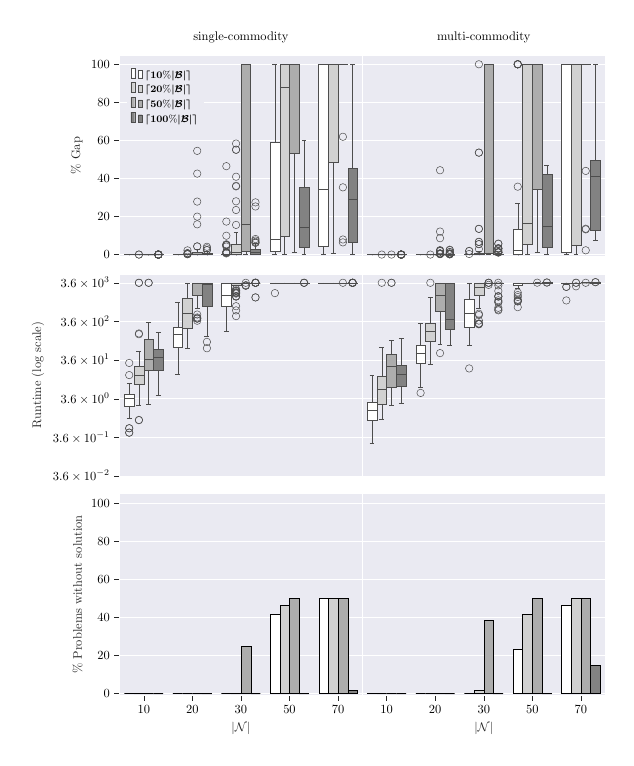
\begin{tikzpicture}[scale=0.45]

\definecolor{darkgray173}{RGB}{173,173,173}
\definecolor{darkslategray38}{RGB}{38,38,38}
\definecolor{darkslategray66}{RGB}{66,66,66}
\definecolor{darkslategray77}{RGB}{77,77,77}
\definecolor{gray130}{RGB}{130,130,130}
\definecolor{lavender234234242}{RGB}{234,234,242}
\definecolor{lightgray209}{RGB}{209,209,209}

\begin{groupplot}[group style={group size=2 by 3, vertical sep=0.5cm, horizontal sep=0pt}]
\nextgroupplot[
axis background/.style={fill=lavender234234242},
axis line style={white},
legend cell align={left},
legend style={
  fill opacity=1,
  draw opacity=1,
  text opacity=1,
  font=\footnotesize,
  at={(0.03,0.95)},
  anchor=north west,
  draw=none,
  fill=lavender234234242
},
scaled x ticks=manual:{}{\pgfmathparse{#1}},
tick align=outside,
title={single-commodity},
x grid style={white},
xmajorticks=false,
xmin=-0.5, xmax=4.5,
xtick style={color=darkslategray38},
xticklabels={},
y grid style={white},
ylabel=\textcolor{darkslategray38}{\% Gap},
ymajorgrids,
ymin=-1, ymax=105,
ytick style={color=darkslategray38},
ytick={0,20,40,60,80,100},
yticklabels={
  \(\displaystyle {0}\),
  \(\displaystyle {20}\),
  \(\displaystyle {40}\),
  \(\displaystyle {60}\),
  \(\displaystyle {80}\),
  \(\displaystyle {100}\)
}
]
\addlegendimage{ybar,ybar legend,draw=white!29.8039215686275!black,fill=white,line width=0.3pt}
\addlegendimage{ybar,ybar legend,draw=white!29.8039215686275!black,fill=lightgray209,line width=0.3pt}
\addlegendimage{ybar,ybar legend,draw=white!29.8039215686275!black,fill=darkgray173,line width=0.3pt}
\addlegendimage{ybar,ybar legend,draw=white!29.8039215686275!black,fill=gray130,line width=0.3pt}
\addlegendentry{$\bm{\lceil 10\%|\mathcal B|\rceil}$}
\addlegendentry{$\bm{\lceil 20\%|\mathcal B|\rceil}$}
\addlegendentry{$\bm{\lceil 50\%|\mathcal B|\rceil}$}
\addlegendentry{$\bm{\lceil 100\%|\mathcal B|\rceil}$}
\path [draw=darkslategray77, fill=white]
(axis cs:-0.4,0.00133572006180106)
--(axis cs:-0.2,0.00133572006180106)
--(axis cs:-0.2,0.00684098458292766)
--(axis cs:-0.4,0.00684098458292766)
--(axis cs:-0.4,0.00133572006180106)
--cycle;
\addplot [darkslategray77, forget plot]
table {%
-0.3 0.00133572006180106
-0.3 0.000120048822704826
};
\addplot [darkslategray77, forget plot]
table {%
-0.3 0.00684098458292766
-0.3 0.00870460190524339
};
\addplot [darkslategray77, forget plot]
table {%
-0.35 0.000120048822704826
-0.25 0.000120048822704826
};
\addplot [darkslategray77, forget plot]
table {%
-0.35 0.00870460190524339
-0.25 0.00870460190524339
};
\path [draw=darkslategray77, fill=white]
(axis cs:0.6,0.000254952071061972)
--(axis cs:0.8,0.000254952071061972)
--(axis cs:0.8,0.00623574733621541)
--(axis cs:0.6,0.00623574733621541)
--(axis cs:0.6,0.000254952071061972)
--cycle;
\addplot [darkslategray77, forget plot]
table {%
0.7 0.000254952071061972
0.7 2.96831508052941e-06
};
\addplot [darkslategray77, forget plot]
table {%
0.7 0.00623574733621541
0.7 0.00990114957427982
};
\addplot [darkslategray77, forget plot]
table {%
0.65 2.96831508052941e-06
0.75 2.96831508052941e-06
};
\addplot [darkslategray77, forget plot]
table {%
0.65 0.00990114957427982
0.75 0.00990114957427982
};
\path [draw=darkslategray77, fill=white]
(axis cs:1.6,0.000562358847510353)
--(axis cs:1.8,0.000562358847510353)
--(axis cs:1.8,0.222906709291283)
--(axis cs:1.6,0.222906709291283)
--(axis cs:1.6,0.000562358847510353)
--cycle;
\addplot [darkslategray77, forget plot]
table {%
1.7 0.000562358847510353
1.7 1.67557903244621e-05
};
\addplot [darkslategray77, forget plot]
table {%
1.7 0.222906709291283
1.7 0.30183320999343
};
\addplot [darkslategray77, forget plot]
table {%
1.65 1.67557903244621e-05
1.75 1.67557903244621e-05
};
\addplot [darkslategray77, forget plot]
table {%
1.65 0.30183320999343
1.75 0.30183320999343
};
\addplot [black, mark=o, mark size=3, mark options={solid,fill opacity=0,draw=darkslategray77}, only marks, forget plot]
table {%
1.7 1.02885889281845
1.7 0.60076572151668
1.7 0.9805006601547
1.7 0.9805006601547
1.7 5.11996796876474
1.7 9.9166998080027
1.7 4.96888717508221
1.7 4.96888717508221
1.7 46.4652765282972
1.7 5.42564185348612
1.7 17.3591362396042
1.7 1.35138624951427
1.7 1.35138624951427
1.7 4.21591215020553
};
\path [draw=darkslategray77, fill=white]
(axis cs:2.6,1.53011653987422)
--(axis cs:2.8,1.53011653987422)
--(axis cs:2.8,59.2055750890407)
--(axis cs:2.6,59.2055750890407)
--(axis cs:2.6,1.53011653987422)
--cycle;
\addplot [darkslategray77, forget plot]
table {%
2.7 1.53011653987422
2.7 0.00074350704463909
};
\addplot [darkslategray77, forget plot]
table {%
2.7 59.2055750890407
2.7 100
};
\addplot [darkslategray77, forget plot]
table {%
2.65 0.00074350704463909
2.75 0.00074350704463909
};
\addplot [darkslategray77, forget plot]
table {%
2.65 100
2.75 100
};
\path [draw=darkslategray77, fill=white]
(axis cs:3.6,4.25114848940175)
--(axis cs:3.8,4.25114848940175)
--(axis cs:3.8,100)
--(axis cs:3.6,100)
--(axis cs:3.6,4.25114848940175)
--cycle;
\addplot [darkslategray77, forget plot]
table {%
3.7 4.25114848940175
3.7 0.248856019288
};
\addplot [darkslategray77, forget plot]
table {%
3.7 100
3.7 100
};
\addplot [darkslategray77, forget plot]
table {%
3.65 0.248856019288
3.75 0.248856019288
};
\addplot [darkslategray77, forget plot]
table {%
3.65 100
3.75 100
};
\path [draw=darkslategray77, fill=lightgray209]
(axis cs:-0.2,0.000247259719623256)
--(axis cs:2.77555756156289e-17,0.000247259719623256)
--(axis cs:2.77555756156289e-17,0.00468073614678733)
--(axis cs:-0.2,0.00468073614678733)
--(axis cs:-0.2,0.000247259719623256)
--cycle;
\addplot [darkslategray77, forget plot]
table {%
-0.1 0.000247259719623256
-0.1 1.08533452078743e-05
};
\addplot [darkslategray77, forget plot]
table {%
-0.1 0.00468073614678733
-0.1 0.00929787727897317
};
\addplot [darkslategray77, forget plot]
table {%
-0.15 1.08533452078743e-05
-0.05 1.08533452078743e-05
};
\addplot [darkslategray77, forget plot]
table {%
-0.15 0.00929787727897317
-0.05 0.00929787727897317
};
\addplot [black, mark=o, mark size=3, mark options={solid,fill opacity=0,draw=darkslategray77}, only marks, forget plot]
table {%
-0.1 0.01716686330995
-0.1 0.02011441348994
};
\path [draw=darkslategray77, fill=lightgray209]
(axis cs:0.8,0.000242995201346606)
--(axis cs:1,0.000242995201346606)
--(axis cs:1,0.00759412710321226)
--(axis cs:0.8,0.00759412710321226)
--(axis cs:0.8,0.000242995201346606)
--cycle;
\addplot [darkslategray77, forget plot]
table {%
0.9 0.000242995201346606
0.9 1.23238990202196e-06
};
\addplot [darkslategray77, forget plot]
table {%
0.9 0.00759412710321226
0.9 0.01703233047422
};
\addplot [darkslategray77, forget plot]
table {%
0.85 1.23238990202196e-06
0.95 1.23238990202196e-06
};
\addplot [darkslategray77, forget plot]
table {%
0.85 0.01703233047422
0.95 0.01703233047422
};
\addplot [black, mark=o, mark size=3, mark options={solid,fill opacity=0,draw=darkslategray77}, only marks, forget plot]
table {%
0.9 0.38095591660376
0.9 2.22699430432005
0.9 0.74929264773176
0.9 0.74888508448456
0.9 0.21258481573405
0.9 0.20951223165075
};
\path [draw=darkslategray77, fill=lightgray209]
(axis cs:1.8,0.00987989592087286)
--(axis cs:2,0.00987989592087286)
--(axis cs:2,5.48297297678599)
--(axis cs:1.8,5.48297297678599)
--(axis cs:1.8,0.00987989592087286)
--cycle;
\addplot [darkslategray77, forget plot]
table {%
1.9 0.00987989592087286
1.9 1.73791944892168e-05
};
\addplot [darkslategray77, forget plot]
table {%
1.9 5.48297297678599
1.9 11.9890325401032
};
\addplot [darkslategray77, forget plot]
table {%
1.85 1.73791944892168e-05
1.95 1.73791944892168e-05
};
\addplot [darkslategray77, forget plot]
table {%
1.85 11.9890325401032
1.95 11.9890325401032
};
\addplot [black, mark=o, mark size=3, mark options={solid,fill opacity=0,draw=darkslategray77}, only marks, forget plot]
table {%
1.9 23.4357479559391
1.9 15.6159206199839
1.9 58.3387306181939
1.9 28.0140586931555
1.9 55.0909518040008
1.9 55.0927304097178
1.9 35.8462454472341
1.9 40.9101694279538
1.9 36.1317828429306
};
\path [draw=darkslategray77, fill=lightgray209]
(axis cs:2.8,9.71663753424275)
--(axis cs:3,9.71663753424275)
--(axis cs:3,100)
--(axis cs:2.8,100)
--(axis cs:2.8,9.71663753424275)
--cycle;
\addplot [darkslategray77, forget plot]
table {%
2.9 9.71663753424275
2.9 0.12584182964922
};
\addplot [darkslategray77, forget plot]
table {%
2.9 100
2.9 100
};
\addplot [darkslategray77, forget plot]
table {%
2.85 0.12584182964922
2.95 0.12584182964922
};
\addplot [darkslategray77, forget plot]
table {%
2.85 100
2.95 100
};
\path [draw=darkslategray77, fill=lightgray209]
(axis cs:3.8,48.6052318998015)
--(axis cs:4,48.6052318998015)
--(axis cs:4,100)
--(axis cs:3.8,100)
--(axis cs:3.8,48.6052318998015)
--cycle;
\addplot [darkslategray77, forget plot]
table {%
3.9 48.6052318998015
3.9 0.58106318778614
};
\addplot [darkslategray77, forget plot]
table {%
3.9 100
3.9 100
};
\addplot [darkslategray77, forget plot]
table {%
3.85 0.58106318778614
3.95 0.58106318778614
};
\addplot [darkslategray77, forget plot]
table {%
3.85 100
3.95 100
};
\path [draw=darkslategray77, fill=darkgray173]
(axis cs:-2.77555756156289e-17,0.0013518266019132)
--(axis cs:0.2,0.0013518266019132)
--(axis cs:0.2,0.00833667646345856)
--(axis cs:-2.77555756156289e-17,0.00833667646345856)
--(axis cs:-2.77555756156289e-17,0.0013518266019132)
--cycle;
\addplot [darkslategray77, forget plot]
table {%
0.1 0.0013518266019132
0.1 8.51487799785397e-05
};
\addplot [darkslategray77, forget plot]
table {%
0.1 0.00833667646345856
0.1 0.01647584015881
};
\addplot [darkslategray77, forget plot]
table {%
0.05 8.51487799785397e-05
0.15 8.51487799785397e-05
};
\addplot [darkslategray77, forget plot]
table {%
0.05 0.01647584015881
0.15 0.01647584015881
};
\path [draw=darkslategray77, fill=darkgray173]
(axis cs:1,0.0064119401012708)
--(axis cs:1.2,0.0064119401012708)
--(axis cs:1.2,1.36712634094474)
--(axis cs:1,1.36712634094474)
--(axis cs:1,0.0064119401012708)
--cycle;
\addplot [darkslategray77, forget plot]
table {%
1.1 0.0064119401012708
1.1 2.89466315893147e-05
};
\addplot [darkslategray77, forget plot]
table {%
1.1 1.36712634094474
1.1 2.83799665004793
};
\addplot [darkslategray77, forget plot]
table {%
1.05 2.89466315893147e-05
1.15 2.89466315893147e-05
};
\addplot [darkslategray77, forget plot]
table {%
1.05 2.83799665004793
1.15 2.83799665004793
};
\addplot [black, mark=o, mark size=3, mark options={solid,fill opacity=0,draw=darkslategray77}, only marks, forget plot]
table {%
1.1 15.9186172784106
1.1 27.8573969203345
1.1 42.5477051126761
1.1 19.9498585235363
1.1 54.5096062256846
1.1 4.30846890205483
1.1 4.30277114543275
};
\path [draw=darkslategray77, fill=darkgray173]
(axis cs:2,1.96296880409666)
--(axis cs:2.2,1.96296880409666)
--(axis cs:2.2,100)
--(axis cs:2,100)
--(axis cs:2,1.96296880409666)
--cycle;
\addplot [darkslategray77, forget plot]
table {%
2.1 1.96296880409666
2.1 0.00130978801725279
};
\addplot [darkslategray77, forget plot]
table {%
2.1 100
2.1 100
};
\addplot [darkslategray77, forget plot]
table {%
2.05 0.00130978801725279
2.15 0.00130978801725279
};
\addplot [darkslategray77, forget plot]
table {%
2.05 100
2.15 100
};
\path [draw=darkslategray77, fill=darkgray173]
(axis cs:3,53.0848391812509)
--(axis cs:3.2,53.0848391812509)
--(axis cs:3.2,100)
--(axis cs:3,100)
--(axis cs:3,53.0848391812509)
--cycle;
\addplot [darkslategray77, forget plot]
table {%
3.1 53.0848391812509
3.1 1.25858977847352
};
\addplot [darkslategray77, forget plot]
table {%
3.1 100
3.1 100
};
\addplot [darkslategray77, forget plot]
table {%
3.05 1.25858977847352
3.15 1.25858977847352
};
\addplot [darkslategray77, forget plot]
table {%
3.05 100
3.15 100
};
\path [draw=darkslategray77, fill=darkgray173]
(axis cs:4,100)
--(axis cs:4.2,100)
--(axis cs:4.2,100)
--(axis cs:4,100)
--(axis cs:4,100)
--cycle;
\addplot [darkslategray77, forget plot]
table {%
4.1 100
4.1 100
};
\addplot [darkslategray77, forget plot]
table {%
4.1 100
4.1 100
};
\addplot [darkslategray77, forget plot]
table {%
4.05 100
4.15 100
};
\addplot [darkslategray77, forget plot]
table {%
4.05 100
4.15 100
};
\addplot [black, mark=o, mark size=3, mark options={solid,fill opacity=0,draw=darkslategray77}, only marks, forget plot]
table {%
4.1 61.9081033537891
4.1 35.3449139534798
4.1 7.94402308881415
4.1 6.43011758167309
};
\path [draw=darkslategray77, fill=gray130]
(axis cs:0.2,0)
--(axis cs:0.4,0)
--(axis cs:0.4,0.000145827775743331)
--(axis cs:0.2,0.000145827775743331)
--(axis cs:0.2,0)
--cycle;
\addplot [darkslategray77, forget plot]
table {%
0.3 0
0.3 0
};
\addplot [darkslategray77, forget plot]
table {%
0.3 0.000145827775743331
0.3 0.000202406747495132
};
\addplot [darkslategray77, forget plot]
table {%
0.25 0
0.35 0
};
\addplot [darkslategray77, forget plot]
table {%
0.25 0.000202406747495132
0.35 0.000202406747495132
};
\addplot [black, mark=o, mark size=3, mark options={solid,fill opacity=0,draw=darkslategray77}, only marks, forget plot]
table {%
0.3 0.001048076830305
0.3 0.00653361265226353
0.3 0.00491909477271809
0.3 0.00850280955604399
0.3 0.00653361265226353
0.3 0.00491909477271809
0.3 0.00850280955604399
0.3 0.000764676184473043
0.3 0.000764676184473043
0.3 0.00705493278507827
0.3 0.00869682912931991
0.3 0.00705493278507827
0.3 0.00869682912931991
};
\path [draw=darkslategray77, fill=gray130]
(axis cs:1.2,0.00724102763358259)
--(axis cs:1.4,0.00724102763358259)
--(axis cs:1.4,0.746184766073172)
--(axis cs:1.2,0.746184766073172)
--(axis cs:1.2,0.00724102763358259)
--cycle;
\addplot [darkslategray77, forget plot]
table {%
1.3 0.00724102763358259
1.3 0
};
\addplot [darkslategray77, forget plot]
table {%
1.3 0.746184766073172
1.3 1.63478411512995
};
\addplot [darkslategray77, forget plot]
table {%
1.25 0
1.35 0
};
\addplot [darkslategray77, forget plot]
table {%
1.25 1.63478411512995
1.35 1.63478411512995
};
\addplot [black, mark=o, mark size=3, mark options={solid,fill opacity=0,draw=darkslategray77}, only marks, forget plot]
table {%
1.3 2.3717273331677
1.3 2.37164865736079
1.3 4.10294448576652
1.3 3.3082368144088
};
\path [draw=darkslategray77, fill=gray130]
(axis cs:2.2,0.397819835965295)
--(axis cs:2.4,0.397819835965295)
--(axis cs:2.4,2.68698958808146)
--(axis cs:2.2,2.68698958808146)
--(axis cs:2.2,0.397819835965295)
--cycle;
\addplot [darkslategray77, forget plot]
table {%
2.3 0.397819835965295
2.3 0.00994756655080013
};
\addplot [darkslategray77, forget plot]
table {%
2.3 2.68698958808146
2.3 5.72650709052836
};
\addplot [darkslategray77, forget plot]
table {%
2.25 0.00994756655080013
2.35 0.00994756655080013
};
\addplot [darkslategray77, forget plot]
table {%
2.25 5.72650709052836
2.35 5.72650709052836
};
\addplot [black, mark=o, mark size=3, mark options={solid,fill opacity=0,draw=darkslategray77}, only marks, forget plot]
table {%
2.3 6.21202174014472
2.3 6.21312321689917
2.3 6.70792469350277
2.3 27.4529522129236
2.3 25.2965408171533
2.3 7.4048280957732
2.3 8.18903993807602
};
\path [draw=darkslategray77, fill=gray130]
(axis cs:3.2,3.94549961223222)
--(axis cs:3.4,3.94549961223222)
--(axis cs:3.4,35.4346336578786)
--(axis cs:3.2,35.4346336578786)
--(axis cs:3.2,3.94549961223222)
--cycle;
\addplot [darkslategray77, forget plot]
table {%
3.3 3.94549961223222
3.3 0.25207008902202
};
\addplot [darkslategray77, forget plot]
table {%
3.3 35.4346336578786
3.3 60.2709633434356
};
\addplot [darkslategray77, forget plot]
table {%
3.25 0.25207008902202
3.35 0.25207008902202
};
\addplot [darkslategray77, forget plot]
table {%
3.25 60.2709633434356
3.35 60.2709633434356
};
\path [draw=darkslategray77, fill=gray130]
(axis cs:4.2,6.60121078852159)
--(axis cs:4.4,6.60121078852159)
--(axis cs:4.4,45.4957468162656)
--(axis cs:4.2,45.4957468162656)
--(axis cs:4.2,6.60121078852159)
--cycle;
\addplot [darkslategray77, forget plot]
table {%
4.3 6.60121078852159
4.3 0.41088319841366
};
\addplot [darkslategray77, forget plot]
table {%
4.3 45.4957468162656
4.3 100
};
\addplot [darkslategray77, forget plot]
table {%
4.25 0.41088319841366
4.35 0.41088319841366
};
\addplot [darkslategray77, forget plot]
table {%
4.25 100
4.35 100
};
\addplot [darkslategray77, forget plot]
table {%
-0.4 0.00399222039291947
-0.2 0.00399222039291947
};
\addplot [darkslategray77, forget plot]
table {%
0.6 0.00189081831752816
0.8 0.00189081831752816
};
\addplot [darkslategray77, forget plot]
table {%
1.6 0.00459889079257395
1.8 0.00459889079257395
};
\addplot [darkslategray77, forget plot]
table {%
2.6 7.9764916141835
2.8 7.9764916141835
};
\addplot [darkslategray77, forget plot]
table {%
3.6 34.128347866323
3.8 34.128347866323
};
\addplot [darkslategray77, forget plot]
table {%
-0.2 0.00143702542971448
2.77555756156289e-17 0.00143702542971448
};
\addplot [darkslategray77, forget plot]
table {%
0.8 0.00193273176080315
1 0.00193273176080315
};
\addplot [darkslategray77, forget plot]
table {%
1.8 1.22055759862991
2 1.22055759862991
};
\addplot [darkslategray77, forget plot]
table {%
2.8 88.0832299376624
3 88.0832299376624
};
\addplot [darkslategray77, forget plot]
table {%
3.8 100
4 100
};
\addplot [darkslategray77, forget plot]
table {%
-2.77555756156289e-17 0.00293727312842118
0.2 0.00293727312842118
};
\addplot [darkslategray77, forget plot]
table {%
1 0.02302980506913
1.2 0.02302980506913
};
\addplot [darkslategray77, forget plot]
table {%
2 16.1272489208952
2.2 16.1272489208952
};
\addplot [darkslategray77, forget plot]
table {%
3 100
3.2 100
};
\addplot [darkslategray77, forget plot]
table {%
4 100
4.2 100
};
\addplot [darkslategray77, forget plot]
table {%
0.2 1.93378046994071e-07
0.4 1.93378046994071e-07
};
\addplot [darkslategray77, forget plot]
table {%
1.2 0.0099817835398677
1.4 0.0099817835398677
};
\addplot [darkslategray77, forget plot]
table {%
2.2 1.1639221952958
2.4 1.1639221952958
};
\addplot [darkslategray77, forget plot]
table {%
3.2 14.2988324578223
3.4 14.2988324578223
};
\addplot [darkslategray77, forget plot]
table {%
4.2 29.3165356078277
4.4 29.3165356078277
};

\nextgroupplot[
axis background/.style={fill=lavender234234242},
axis line style={white},
scaled x ticks=manual:{}{\pgfmathparse{#1}},
scaled y ticks=manual:{}{\pgfmathparse{#1}},
tick align=outside,
title={multi-commodity},
x grid style={white},
xmajorticks=false,
xmin=-0.5, xmax=4.5,
xtick style={color=darkslategray38},
xticklabels={},
y grid style={white},
ymajorgrids,
ymajorticks=false,
ymin=-1, ymax=105,
ytick style={color=darkslategray38},
yticklabels={}
]
\path [draw=darkslategray77, fill=white]
(axis cs:-0.4,0.000936504549970713)
--(axis cs:-0.2,0.000936504549970713)
--(axis cs:-0.2,0.00592060246321592)
--(axis cs:-0.4,0.00592060246321592)
--(axis cs:-0.4,0.000936504549970713)
--cycle;
\addplot [darkslategray77]
table {%
-0.3 0.000936504549970713
-0.3 0
};
\addplot [darkslategray77]
table {%
-0.3 0.00592060246321592
-0.3 0.00937719604503964
};
\addplot [darkslategray77]
table {%
-0.35 0
-0.25 0
};
\addplot [darkslategray77]
table {%
-0.35 0.00937719604503964
-0.25 0.00937719604503964
};
\path [draw=darkslategray77, fill=white]
(axis cs:0.6,0.000407243843051177)
--(axis cs:0.8,0.000407243843051177)
--(axis cs:0.8,0.00591544467590321)
--(axis cs:0.6,0.00591544467590321)
--(axis cs:0.6,0.000407243843051177)
--cycle;
\addplot [darkslategray77]
table {%
0.7 0.000407243843051177
0.7 3.20128139152037e-05
};
\addplot [darkslategray77]
table {%
0.7 0.00591544467590321
0.7 0.00984005175301184
};
\addplot [darkslategray77]
table {%
0.65 3.20128139152037e-05
0.75 3.20128139152037e-05
};
\addplot [darkslategray77]
table {%
0.65 0.00984005175301184
0.75 0.00984005175301184
};
\path [draw=darkslategray77, fill=white]
(axis cs:1.6,0.000241661653647296)
--(axis cs:1.8,0.000241661653647296)
--(axis cs:1.8,0.00697323839835158)
--(axis cs:1.6,0.00697323839835158)
--(axis cs:1.6,0.000241661653647296)
--cycle;
\addplot [darkslategray77]
table {%
1.7 0.000241661653647296
1.7 4.57187053933903e-06
};
\addplot [darkslategray77]
table {%
1.7 0.00697323839835158
1.7 0.00994091568627952
};
\addplot [darkslategray77]
table {%
1.65 4.57187053933903e-06
1.75 4.57187053933903e-06
};
\addplot [darkslategray77]
table {%
1.65 0.00994091568627952
1.75 0.00994091568627952
};
\addplot [black, mark=o, mark size=3, mark options={solid,fill opacity=0,draw=darkslategray77}, only marks]
table {%
1.7 1.90534300789556
1.7 1.90077917324969
1.7 0.31236388018016
};
\path [draw=darkslategray77, fill=white]
(axis cs:2.6,0.0081804451944545)
--(axis cs:2.8,0.0081804451944545)
--(axis cs:2.8,13.3956251878068)
--(axis cs:2.6,13.3956251878068)
--(axis cs:2.6,0.0081804451944545)
--cycle;
\addplot [darkslategray77]
table {%
2.7 0.0081804451944545
2.7 4.00654585343835e-05
};
\addplot [darkslategray77]
table {%
2.7 13.3956251878068
2.7 26.9852998076058
};
\addplot [darkslategray77]
table {%
2.65 4.00654585343835e-05
2.75 4.00654585343835e-05
};
\addplot [darkslategray77]
table {%
2.65 26.9852998076058
2.75 26.9852998076058
};
\addplot [black, mark=o, mark size=3, mark options={solid,fill opacity=0,draw=darkslategray77}, only marks]
table {%
2.7 100
2.7 100
2.7 100
2.7 100
2.7 35.6824211954955
2.7 100
};
\path [draw=darkslategray77, fill=white]
(axis cs:3.6,1.15405524523183)
--(axis cs:3.8,1.15405524523183)
--(axis cs:3.8,100)
--(axis cs:3.6,100)
--(axis cs:3.6,1.15405524523183)
--cycle;
\addplot [darkslategray77]
table {%
3.7 1.15405524523183
3.7 0.000638959375493919
};
\addplot [darkslategray77]
table {%
3.7 100
3.7 100
};
\addplot [darkslategray77]
table {%
3.65 0.000638959375493919
3.75 0.000638959375493919
};
\addplot [darkslategray77]
table {%
3.65 100
3.75 100
};
\path [draw=darkslategray77, fill=lightgray209]
(axis cs:-0.2,0.00154861461287121)
--(axis cs:2.77555756156289e-17,0.00154861461287121)
--(axis cs:2.77555756156289e-17,0.00656948554448497)
--(axis cs:-0.2,0.00656948554448497)
--(axis cs:-0.2,0.00154861461287121)
--cycle;
\addplot [darkslategray77]
table {%
-0.1 0.00154861461287121
-0.1 6.88867011275165e-05
};
\addplot [darkslategray77]
table {%
-0.1 0.00656948554448497
-0.1 0.00977473330891838
};
\addplot [darkslategray77]
table {%
-0.15 6.88867011275165e-05
-0.05 6.88867011275165e-05
};
\addplot [darkslategray77]
table {%
-0.15 0.00977473330891838
-0.05 0.00977473330891838
};
\addplot [black, mark=o, mark size=3, mark options={solid,fill opacity=0,draw=darkslategray77}, only marks]
table {%
-0.1 0.01590952346553
};
\path [draw=darkslategray77, fill=lightgray209]
(axis cs:0.8,0.000260778705829717)
--(axis cs:1,0.000260778705829717)
--(axis cs:1,0.00768718128643697)
--(axis cs:0.8,0.00768718128643697)
--(axis cs:0.8,0.000260778705829717)
--cycle;
\addplot [darkslategray77]
table {%
0.9 0.000260778705829717
0.9 3.6778828221793e-06
};
\addplot [darkslategray77]
table {%
0.9 0.00768718128643697
0.9 0.00998124249766156
};
\addplot [darkslategray77]
table {%
0.85 3.6778828221793e-06
0.95 3.6778828221793e-06
};
\addplot [darkslategray77]
table {%
0.85 0.00998124249766156
0.95 0.00998124249766156
};
\addplot [black, mark=o, mark size=3, mark options={solid,fill opacity=0,draw=darkslategray77}, only marks]
table {%
0.9 0.0199753180264
};
\path [draw=darkslategray77, fill=lightgray209]
(axis cs:1.8,0.00248497636587316)
--(axis cs:2,0.00248497636587316)
--(axis cs:2,0.74230702775802)
--(axis cs:1.8,0.74230702775802)
--(axis cs:1.8,0.00248497636587316)
--cycle;
\addplot [darkslategray77]
table {%
1.9 0.00248497636587316
1.9 1.23694643955478e-08
};
\addplot [darkslategray77]
table {%
1.9 0.74230702775802
1.9 1.64584896522266
};
\addplot [darkslategray77]
table {%
1.85 1.23694643955478e-08
1.95 1.23694643955478e-08
};
\addplot [darkslategray77]
table {%
1.85 1.64584896522266
1.95 1.64584896522266
};
\addplot [black, mark=o, mark size=3, mark options={solid,fill opacity=0,draw=darkslategray77}, only marks]
table {%
1.9 5.50118923455796
1.9 5.50118923455796
1.9 53.5661945854495
1.9 53.5660174944889
1.9 13.5254016361461
1.9 13.5254016361461
1.9 2.93672402541584
1.9 6.70614284710501
1.9 6.70614284710501
1.9 100
};
\path [draw=darkslategray77, fill=lightgray209]
(axis cs:2.8,5.56352097973851)
--(axis cs:3,5.56352097973851)
--(axis cs:3,100)
--(axis cs:2.8,100)
--(axis cs:2.8,5.56352097973851)
--cycle;
\addplot [darkslategray77]
table {%
2.9 5.56352097973851
2.9 0.09867883290345
};
\addplot [darkslategray77]
table {%
2.9 100
2.9 100
};
\addplot [darkslategray77]
table {%
2.85 0.09867883290345
2.95 0.09867883290345
};
\addplot [darkslategray77]
table {%
2.85 100
2.95 100
};
\path [draw=darkslategray77, fill=lightgray209]
(axis cs:3.8,5.11837783070905)
--(axis cs:4,5.11837783070905)
--(axis cs:4,100)
--(axis cs:3.8,100)
--(axis cs:3.8,5.11837783070905)
--cycle;
\addplot [darkslategray77]
table {%
3.9 5.11837783070905
3.9 0.00871839567541549
};
\addplot [darkslategray77]
table {%
3.9 100
3.9 100
};
\addplot [darkslategray77]
table {%
3.85 0.00871839567541549
3.95 0.00871839567541549
};
\addplot [darkslategray77]
table {%
3.85 100
3.95 100
};
\path [draw=darkslategray77, fill=darkgray173]
(axis cs:-2.77555756156289e-17,0.00114440762850478)
--(axis cs:0.2,0.00114440762850478)
--(axis cs:0.2,0.00710276699396135)
--(axis cs:-2.77555756156289e-17,0.00710276699396135)
--(axis cs:-2.77555756156289e-17,0.00114440762850478)
--cycle;
\addplot [darkslategray77]
table {%
0.1 0.00114440762850478
0.1 7.91082337593064e-05
};
\addplot [darkslategray77]
table {%
0.1 0.00710276699396135
0.1 0.01413024739351
};
\addplot [darkslategray77]
table {%
0.05 7.91082337593064e-05
0.15 7.91082337593064e-05
};
\addplot [darkslategray77]
table {%
0.05 0.01413024739351
0.15 0.01413024739351
};
\addplot [black, mark=o, mark size=3, mark options={solid,fill opacity=0,draw=darkslategray77}, only marks]
table {%
0.1 0.01799198308724
};
\path [draw=darkslategray77, fill=darkgray173]
(axis cs:1,0.00533362081853075)
--(axis cs:1.2,0.00533362081853075)
--(axis cs:1.2,0.026265792848975)
--(axis cs:1,0.026265792848975)
--(axis cs:1,0.00533362081853075)
--cycle;
\addplot [darkslategray77]
table {%
1.1 0.00533362081853075
1.1 6.6745668083e-06
};
\addplot [darkslategray77]
table {%
1.1 0.026265792848975
1.1 0.03740799805625
};
\addplot [darkslategray77]
table {%
1.05 6.6745668083e-06
1.15 6.6745668083e-06
};
\addplot [darkslategray77]
table {%
1.05 0.03740799805625
1.15 0.03740799805625
};
\addplot [black, mark=o, mark size=3, mark options={solid,fill opacity=0,draw=darkslategray77}, only marks]
table {%
1.1 0.61388790345455
1.1 0.62384437181204
1.1 1.91938548962605
1.1 1.91938548962605
1.1 8.62113243239045
1.1 0.23583848829861
1.1 12.1129478137183
1.1 1.96255133639009
1.1 2.35062797140051
1.1 44.3304667808476
1.1 0.30945342925767
1.1 0.53387621696224
1.1 0.39679228038132
1.1 0.39317800201087
};
\path [draw=darkslategray77, fill=darkgray173]
(axis cs:2,0.95183679858894)
--(axis cs:2.2,0.95183679858894)
--(axis cs:2.2,100)
--(axis cs:2,100)
--(axis cs:2,0.95183679858894)
--cycle;
\addplot [darkslategray77]
table {%
2.1 0.95183679858894
2.1 0.00234961721279486
};
\addplot [darkslategray77]
table {%
2.1 100
2.1 100
};
\addplot [darkslategray77]
table {%
2.05 0.00234961721279486
2.15 0.00234961721279486
};
\addplot [darkslategray77]
table {%
2.05 100
2.15 100
};
\path [draw=darkslategray77, fill=darkgray173]
(axis cs:3,34.0822784576997)
--(axis cs:3.2,34.0822784576997)
--(axis cs:3.2,100)
--(axis cs:3,100)
--(axis cs:3,34.0822784576997)
--cycle;
\addplot [darkslategray77]
table {%
3.1 34.0822784576997
3.1 1.2567769263594
};
\addplot [darkslategray77]
table {%
3.1 100
3.1 100
};
\addplot [darkslategray77]
table {%
3.05 1.2567769263594
3.15 1.2567769263594
};
\addplot [darkslategray77]
table {%
3.05 100
3.15 100
};
\path [draw=darkslategray77, fill=darkgray173]
(axis cs:4,100)
--(axis cs:4.2,100)
--(axis cs:4.2,100)
--(axis cs:4,100)
--(axis cs:4,100)
--cycle;
\addplot [darkslategray77]
table {%
4.1 100
4.1 100
};
\addplot [darkslategray77]
table {%
4.1 100
4.1 100
};
\addplot [darkslategray77]
table {%
4.05 100
4.15 100
};
\addplot [darkslategray77]
table {%
4.05 100
4.15 100
};
\addplot [black, mark=o, mark size=3, mark options={solid,fill opacity=0,draw=darkslategray77}, only marks]
table {%
4.1 13.2599453371266
4.1 2.26308473023633
4.1 43.9660512515118
4.1 13.5842873266244
};
\path [draw=darkslategray77, fill=gray130]
(axis cs:0.2,1.0049557904745e-07)
--(axis cs:0.4,1.0049557904745e-07)
--(axis cs:0.4,0.00109313773159634)
--(axis cs:0.2,0.00109313773159634)
--(axis cs:0.2,1.0049557904745e-07)
--cycle;
\addplot [darkslategray77]
table {%
0.3 1.0049557904745e-07
0.3 0
};
\addplot [darkslategray77]
table {%
0.3 0.00109313773159634
0.3 0.00163121067277202
};
\addplot [darkslategray77]
table {%
0.25 0
0.35 0
};
\addplot [darkslategray77]
table {%
0.25 0.00163121067277202
0.35 0.00163121067277202
};
\addplot [black, mark=o, mark size=3, mark options={solid,fill opacity=0,draw=darkslategray77}, only marks]
table {%
0.3 0.00768620894099423
0.3 0.00786959194415094
0.3 0.00768620894099423
0.3 0.00786959194415094
0.3 0.00364254781490621
0.3 0.00734107102951364
0.3 0.00364254781490621
0.3 0.00734107102951364
0.3 0.00943206025384057
0.3 0.0037125738539398
0.3 0.00951963296112049
0.3 0.00951963296112049
};
\path [draw=darkslategray77, fill=gray130]
(axis cs:1.2,0.00471202400607463)
--(axis cs:1.4,0.00471202400607463)
--(axis cs:1.4,0.0533162847191675)
--(axis cs:1.2,0.0533162847191675)
--(axis cs:1.2,0.00471202400607463)
--cycle;
\addplot [darkslategray77]
table {%
1.3 0.00471202400607463
1.3 0
};
\addplot [darkslategray77]
table {%
1.3 0.0533162847191675
1.3 0.09435639153841
};
\addplot [darkslategray77]
table {%
1.25 0
1.35 0
};
\addplot [darkslategray77]
table {%
1.25 0.09435639153841
1.35 0.09435639153841
};
\addplot [black, mark=o, mark size=3, mark options={solid,fill opacity=0,draw=darkslategray77}, only marks]
table {%
1.3 1.29757129646422
1.3 1.37785897890718
1.3 2.34491626469436
1.3 2.56029347961817
1.3 0.52348045158277
1.3 0.62805717715904
1.3 0.14930669918111
1.3 0.18530927827884
1.3 0.26247043734633
1.3 0.37572560617582
1.3 0.39094093914639
};
\path [draw=darkslategray77, fill=gray130]
(axis cs:2.2,0.021477626805395)
--(axis cs:2.4,0.021477626805395)
--(axis cs:2.4,0.409402661032715)
--(axis cs:2.2,0.409402661032715)
--(axis cs:2.2,0.021477626805395)
--cycle;
\addplot [darkslategray77]
table {%
2.3 0.021477626805395
2.3 0.00106314200838244
};
\addplot [darkslategray77]
table {%
2.3 0.409402661032715
2.3 0.70966022681049
};
\addplot [darkslategray77]
table {%
2.25 0.00106314200838244
2.35 0.00106314200838244
};
\addplot [darkslategray77]
table {%
2.25 0.70966022681049
2.35 0.70966022681049
};
\addplot [black, mark=o, mark size=3, mark options={solid,fill opacity=0,draw=darkslategray77}, only marks]
table {%
2.3 5.64452209279346
2.3 5.78034398464468
2.3 3.12081731261197
2.3 2.97995329446986
2.3 3.36369177194993
2.3 3.36369177194993
2.3 1.25531680705684
2.3 1.25665177062541
2.3 2.02327688549173
2.3 1.03314121672981
2.3 1.28736985216044
2.3 1.25983011206012
};
\path [draw=darkslategray77, fill=gray130]
(axis cs:3.2,3.80163321363401)
--(axis cs:3.4,3.80163321363401)
--(axis cs:3.4,42.155290083801)
--(axis cs:3.2,42.155290083801)
--(axis cs:3.2,3.80163321363401)
--cycle;
\addplot [darkslategray77]
table {%
3.3 3.80163321363401
3.3 0.05551999703634
};
\addplot [darkslategray77]
table {%
3.3 42.155290083801
3.3 46.9113227056868
};
\addplot [darkslategray77]
table {%
3.25 0.05551999703634
3.35 0.05551999703634
};
\addplot [darkslategray77]
table {%
3.25 46.9113227056868
3.35 46.9113227056868
};
\path [draw=darkslategray77, fill=gray130]
(axis cs:4.2,12.8256961396406)
--(axis cs:4.4,12.8256961396406)
--(axis cs:4.4,49.6067742095386)
--(axis cs:4.2,49.6067742095386)
--(axis cs:4.2,12.8256961396406)
--cycle;
\addplot [darkslategray77]
table {%
4.3 12.8256961396406
4.3 7.3079891542194
};
\addplot [darkslategray77]
table {%
4.3 49.6067742095386
4.3 100
};
\addplot [darkslategray77]
table {%
4.25 7.3079891542194
4.35 7.3079891542194
};
\addplot [darkslategray77]
table {%
4.25 100
4.35 100
};
\addplot [darkslategray77]
table {%
-0.4 0.00282784718606901
-0.2 0.00282784718606901
};
\addplot [darkslategray77]
table {%
0.6 0.0014078728965809
0.8 0.0014078728965809
};
\addplot [darkslategray77]
table {%
1.6 0.00398310359421022
1.8 0.00398310359421022
};
\addplot [darkslategray77]
table {%
2.6 2.21044658750946
2.8 2.21044658750946
};
\addplot [darkslategray77]
table {%
3.6 100
3.8 100
};
\addplot [darkslategray77]
table {%
-0.2 0.00411323950857388
2.77555756156289e-17 0.00411323950857388
};
\addplot [darkslategray77]
table {%
0.8 0.00161996474003499
1 0.00161996474003499
};
\addplot [darkslategray77]
table {%
1.8 0.00781476341704454
2 0.00781476341704454
};
\addplot [darkslategray77]
table {%
2.8 16.7237582410889
3 16.7237582410889
};
\addplot [darkslategray77]
table {%
3.8 100
4 100
};
\addplot [darkslategray77]
table {%
-2.77555756156289e-17 0.00416158128801503
0.2 0.00416158128801503
};
\addplot [darkslategray77]
table {%
1 0.00938617390992538
1.2 0.00938617390992538
};
\addplot [darkslategray77]
table {%
2 100
2.2 100
};
\addplot [darkslategray77]
table {%
3 100
3.2 100
};
\addplot [darkslategray77]
table {%
4 100
4.2 100
};
\addplot [darkslategray77]
table {%
0.2 7.42815763539642e-05
0.4 7.42815763539642e-05
};
\addplot [darkslategray77]
table {%
1.2 0.00906736618510651
1.4 0.00906736618510651
};
\addplot [darkslategray77]
table {%
2.2 0.191838012860425
2.4 0.191838012860425
};
\addplot [darkslategray77]
table {%
3.2 15.0745383364631
3.4 15.0745383364631
};
\addplot [darkslategray77]
table {%
4.2 41.4203741441358
4.4 41.4203741441358
};

\nextgroupplot[
axis background/.style={fill=lavender234234242},
axis line style={white},
log basis y={10},
scaled x ticks=manual:{}{\pgfmathparse{#1}},
scaled y ticks=manual:{}{\pgfmathparse{#1}},
tick align=outside,
x grid style={white},
xmajorticks=false,
xmin=-0.5, xmax=4.5,
xtick style={color=darkslategray38},
xticklabels={},
y grid style={white},
ylabel=\textcolor{darkslategray38}{Runtime (log scale)},
ymajorgrids,
ymajorticks,
ymin=0.036, ymax=6000,
ymode=log,
ytick style={color=darkslategray38},
ytick={0.036,0.36,3.6,36,360,3600},
yticklabels={
  \(\displaystyle 3.6\times 10^{-2}\),
  \(\displaystyle 3.6\times 10^{-1}\),
  \(\displaystyle 3.6\times 10^{0}\),
  \(\displaystyle 3.6\times 10^{1}\),
  \(\displaystyle 3.6\times 10^{2}\),
  \(\displaystyle 3.6\times 10^{3}\)
}
]
\path [draw=darkslategray77, fill=white]
(axis cs:-0.4,2.26871116595419)
--(axis cs:-0.2,2.26871116595419)
--(axis cs:-0.2,4.76754151291447)
--(axis cs:-0.4,4.76754151291447)
--(axis cs:-0.4,2.26871116595419)
--cycle;
\addplot [darkslategray77]
table {%
-0.3 2.26871116595419
-0.3 1.09869289398193
};
\addplot [darkslategray77]
table {%
-0.3 4.76754151291447
-0.3 9.1506199836731
};
\addplot [darkslategray77]
table {%
-0.35 1.09869289398193
-0.25 1.09869289398193
};
\addplot [darkslategray77]
table {%
-0.35 9.1506199836731
-0.25 9.1506199836731
};
\addplot [black, mark=o, mark size=3, mark options={solid,fill opacity=0,draw=darkslategray77}, only marks]
table {%
-0.3 0.617192983627319
-0.3 0.473899841308594
-0.3 0.620143175125122
-0.3 0.477431058883667
-0.3 30.2641580104828
-0.3 14.7258040904999
};
\path [draw=darkslategray77, fill=white]
(axis cs:0.6,77.3099636662638)
--(axis cs:0.8,77.3099636662638)
--(axis cs:0.8,260.445650918301)
--(axis cs:0.6,260.445650918301)
--(axis cs:0.6,77.3099636662638)
--cycle;
\addplot [darkslategray77]
table {%
0.7 77.3099636662638
0.7 15.6860361099243
};
\addplot [darkslategray77]
table {%
0.7 260.445650918301
0.7 1144.18928813934
};
\addplot [darkslategray77]
table {%
0.65 15.6860361099243
0.75 15.6860361099243
};
\addplot [darkslategray77]
table {%
0.65 1144.18928813934
0.75 1144.18928813934
};
\path [draw=darkslategray77, fill=white]
(axis cs:1.6,887.369805222838)
--(axis cs:1.8,887.369805222838)
--(axis cs:1.8,3600.09827303535)
--(axis cs:1.6,3600.09827303535)
--(axis cs:1.6,887.369805222838)
--cycle;
\addplot [darkslategray77]
table {%
1.7 887.369805222838
1.7 196.345447063446
};
\addplot [darkslategray77]
table {%
1.7 3600.09827303535
1.7 3600.38953495026
};
\addplot [darkslategray77]
table {%
1.65 196.345447063446
1.75 196.345447063446
};
\addplot [darkslategray77]
table {%
1.65 3600.38953495026
1.75 3600.38953495026
};
\path [draw=darkslategray77, fill=white]
(axis cs:2.6,3600.22683791576)
--(axis cs:2.8,3600.22683791576)
--(axis cs:2.8,3600.38084149105)
--(axis cs:2.6,3600.38084149105)
--(axis cs:2.6,3600.22683791576)
--cycle;
\addplot [darkslategray77]
table {%
2.7 3600.22683791576
2.7 3600.03791594505
};
\addplot [darkslategray77]
table {%
2.7 3600.38084149105
2.7 3600.42983412743
};
\addplot [darkslategray77]
table {%
2.65 3600.03791594505
2.75 3600.03791594505
};
\addplot [darkslategray77]
table {%
2.65 3600.42983412743
2.75 3600.42983412743
};
\addplot [black, mark=o, mark size=3, mark options={solid,fill opacity=0,draw=darkslategray77}, only marks]
table {%
2.7 1945.18206906319
};
\path [draw=darkslategray77, fill=white]
(axis cs:3.6,3600.22122492673)
--(axis cs:3.8,3600.22122492673)
--(axis cs:3.8,3600.79170381084)
--(axis cs:3.6,3600.79170381084)
--(axis cs:3.6,3600.22122492673)
--cycle;
\addplot [darkslategray77]
table {%
3.7 3600.22122492673
3.7 3600.10244584084
};
\addplot [darkslategray77]
table {%
3.7 3600.79170381084
3.7 3600.94338703156
};
\addplot [darkslategray77]
table {%
3.65 3600.10244584084
3.75 3600.10244584084
};
\addplot [darkslategray77]
table {%
3.65 3600.94338703156
3.75 3600.94338703156
};
\path [draw=darkslategray77, fill=lightgray209]
(axis cs:-0.2,8.33520474274839)
--(axis cs:2.77555756156289e-17,8.33520474274839)
--(axis cs:2.77555756156289e-17,25.3832988478104)
--(axis cs:-0.2,25.3832988478104)
--(axis cs:-0.2,8.33520474274839)
--cycle;
\addplot [darkslategray77]
table {%
-0.1 8.33520474274839
-0.1 2.46667194366455
};
\addplot [darkslategray77]
table {%
-0.1 25.3832988478104
-0.1 59.106782913208
};
\addplot [darkslategray77]
table {%
-0.15 2.46667194366455
-0.05 2.46667194366455
};
\addplot [darkslategray77]
table {%
-0.15 59.106782913208
-0.05 59.106782913208
};
\addplot [black, mark=o, mark size=3, mark options={solid,fill opacity=0,draw=darkslategray77}, only marks]
table {%
-0.1 1.01596307754517
-0.1 1.00122499465942
-0.1 167.959690093994
-0.1 175.893085956574
-0.1 3600.01144719124
-0.1 3600.01951599121
};
\path [draw=darkslategray77, fill=lightgray209]
(axis cs:0.8,237.878643921998)
--(axis cs:1,237.878643921998)
--(axis cs:1,1472.45856363723)
--(axis cs:0.8,1472.45856363723)
--(axis cs:0.8,237.878643921998)
--cycle;
\addplot [darkslategray77]
table {%
0.9 237.878643921998
0.9 73.853630065918
};
\addplot [darkslategray77]
table {%
0.9 1472.45856363723
0.9 3600.1668870449
};
\addplot [darkslategray77]
table {%
0.85 73.853630065918
0.95 73.853630065918
};
\addplot [darkslategray77]
table {%
0.85 3600.1668870449
0.95 3600.1668870449
};
\path [draw=darkslategray77, fill=lightgray209]
(axis cs:1.8,3157.52907811968)
--(axis cs:2,3157.52907811968)
--(axis cs:2,3600.21001505835)
--(axis cs:1.8,3600.21001505835)
--(axis cs:1.8,3157.52907811968)
--cycle;
\addplot [darkslategray77]
table {%
1.9 3157.52907811968
1.9 3154.87415504456
};
\addplot [darkslategray77]
table {%
1.9 3600.21001505835
1.9 3600.2913839817
};
\addplot [darkslategray77]
table {%
1.85 3154.87415504456
1.95 3154.87415504456
};
\addplot [darkslategray77]
table {%
1.85 3600.2913839817
1.95 3600.2913839817
};
\addplot [black, mark=o, mark size=3, mark options={solid,fill opacity=0,draw=darkslategray77}, only marks]
table {%
1.9 2046.05478405952
1.9 1579.55667614937
1.9 1609.09844398499
1.9 1892.75414299965
1.9 695.234676837921
1.9 493.595369815826
1.9 1993.0731189251
1.9 1966.48952293396
1.9 1607.5165450573
1.9 2288.26890802384
1.9 2228.46240711212
1.9 2190.32612490654
1.9 891.37403512001
1.9 2482.00583004951
};
\path [draw=darkslategray77, fill=lightgray209]
(axis cs:2.8,3600.17615949141)
--(axis cs:3,3600.17615949141)
--(axis cs:3,3600.53815602007)
--(axis cs:2.8,3600.53815602007)
--(axis cs:2.8,3600.17615949141)
--cycle;
\addplot [darkslategray77]
table {%
2.9 3600.17615949141
2.9 3600.09494209289
};
\addplot [darkslategray77]
table {%
2.9 3600.53815602007
2.9 3600.98611402512
};
\addplot [darkslategray77]
table {%
2.85 3600.09494209289
2.95 3600.09494209289
};
\addplot [darkslategray77]
table {%
2.85 3600.98611402512
2.95 3600.98611402512
};
\path [draw=darkslategray77, fill=lightgray209]
(axis cs:3.8,3600.39331817627)
--(axis cs:4,3600.39331817627)
--(axis cs:4,3601.03802800179)
--(axis cs:3.8,3601.03802800179)
--(axis cs:3.8,3600.39331817627)
--cycle;
\addplot [darkslategray77]
table {%
3.9 3600.39331817627
3.9 3600.2157459259
};
\addplot [darkslategray77]
table {%
3.9 3601.03802800179
3.9 3601.09951591492
};
\addplot [darkslategray77]
table {%
3.85 3600.2157459259
3.95 3600.2157459259
};
\addplot [darkslategray77]
table {%
3.85 3601.09951591492
3.95 3601.09951591492
};
\path [draw=darkslategray77, fill=darkgray173]
(axis cs:-2.77555756156289e-17,20.2039631270003)
--(axis cs:0.2,20.2039631270003)
--(axis cs:0.2,124.006682726397)
--(axis cs:-2.77555756156289e-17,124.006682726397)
--(axis cs:-2.77555756156289e-17,20.2039631270003)
--cycle;
\addplot [darkslategray77]
table {%
0.1 20.2039631270003
0.1 2.59157299995422
};
\addplot [darkslategray77]
table {%
0.1 124.006682726397
0.1 340.912337779999
};
\addplot [darkslategray77]
table {%
0.05 2.59157299995422
0.15 2.59157299995422
};
\addplot [darkslategray77]
table {%
0.05 340.912337779999
0.15 340.912337779999
};
\addplot [black, mark=o, mark size=3, mark options={solid,fill opacity=0,draw=darkslategray77}, only marks]
table {%
0.1 3600.02227306366
0.1 3600.0270459652
};
\path [draw=darkslategray77, fill=darkgray173]
(axis cs:1,1689.99149130065)
--(axis cs:1.2,1689.99149130065)
--(axis cs:1.2,3600.16391092539)
--(axis cs:1,3600.16391092539)
--(axis cs:1,1689.99149130065)
--cycle;
\addplot [darkslategray77]
table {%
1.1 1689.99149130065
1.1 795.696887016297
};
\addplot [darkslategray77]
table {%
1.1 3600.16391092539
1.1 3600.36510300636
};
\addplot [darkslategray77]
table {%
1.05 795.696887016297
1.15 795.696887016297
};
\addplot [darkslategray77]
table {%
1.05 3600.36510300636
1.15 3600.36510300636
};
\addplot [black, mark=o, mark size=3, mark options={solid,fill opacity=0,draw=darkslategray77}, only marks]
table {%
1.1 430.655117034912
1.1 375.4549908638
1.1 424.614044904709
1.1 428.012333869934
1.1 543.191950082779
1.1 455.883782148361
};
\path [draw=darkslategray77, fill=darkgray173]
(axis cs:2,3600.29157740917)
--(axis cs:2.2,3600.29157740917)
--(axis cs:2.2,3600.38892006606)
--(axis cs:2,3600.38892006606)
--(axis cs:2,3600.29157740917)
--cycle;
\addplot [darkslategray77]
table {%
2.1 3600.29157740917
2.1 3600.24243617058
};
\addplot [darkslategray77]
table {%
2.1 3600.38892006606
2.1 3600.51521015167
};
\addplot [darkslategray77]
table {%
2.05 3600.24243617058
2.15 3600.24243617058
};
\addplot [darkslategray77]
table {%
2.05 3600.51521015167
2.15 3600.51521015167
};
\addplot [black, mark=o, mark size=3, mark options={solid,fill opacity=0,draw=darkslategray77}, only marks]
table {%
2.1 3047.2943880558
2.1 3008.49679899216
2.1 3133.10526418686
2.1 3600.53529310226
};
\path [draw=darkslategray77, fill=darkgray173]
(axis cs:3,3600.189507067)
--(axis cs:3.2,3600.189507067)
--(axis cs:3.2,3600.83749113805)
--(axis cs:3,3600.83749113805)
--(axis cs:3,3600.189507067)
--cycle;
\addplot [darkslategray77]
table {%
3.1 3600.189507067
3.1 3600.13245105743
};
\addplot [darkslategray77]
table {%
3.1 3600.83749113805
3.1 3601.18598079682
};
\addplot [darkslategray77]
table {%
3.05 3600.13245105743
3.15 3600.13245105743
};
\addplot [darkslategray77]
table {%
3.05 3601.18598079682
3.15 3601.18598079682
};
\path [draw=darkslategray77, fill=darkgray173]
(axis cs:4,3600.31053116961)
--(axis cs:4.2,3600.31053116961)
--(axis cs:4.2,3600.66944265287)
--(axis cs:4,3600.66944265287)
--(axis cs:4,3600.31053116961)
--cycle;
\addplot [darkslategray77]
table {%
4.1 3600.31053116961
4.1 3600.25388002396
};
\addplot [darkslategray77]
table {%
4.1 3600.66944265287
4.1 3600.66944265287
};
\addplot [darkslategray77]
table {%
4.05 3600.25388002396
4.15 3600.25388002396
};
\addplot [darkslategray77]
table {%
4.05 3600.66944265287
4.15 3600.66944265287
};
\addplot [black, mark=o, mark size=3, mark options={solid,fill opacity=0,draw=darkslategray77}, only marks]
table {%
4.1 3601.6182858944
};
\path [draw=darkslategray77, fill=gray130]
(axis cs:0.2,19.9925807385774)
--(axis cs:0.4,19.9925807385774)
--(axis cs:0.4,70.4890854878717)
--(axis cs:0.2,70.4890854878717)
--(axis cs:0.2,19.9925807385774)
--cycle;
\addplot [darkslategray77]
table {%
0.3 19.9925807385774
0.3 4.37386703491211
};
\addplot [darkslategray77]
table {%
0.3 70.4890854878717
0.3 186.300193071365
};
\addplot [darkslategray77]
table {%
0.25 4.37386703491211
0.35 4.37386703491211
};
\addplot [darkslategray77]
table {%
0.25 186.300193071365
0.35 186.300193071365
};
\path [draw=darkslategray77, fill=gray130]
(axis cs:1.2,891.933046481747)
--(axis cs:1.4,891.933046481747)
--(axis cs:1.4,3600.23272299543)
--(axis cs:1.2,3600.23272299543)
--(axis cs:1.2,891.933046481747)
--cycle;
\addplot [darkslategray77]
table {%
1.3 891.933046481747
1.3 148.55437707901
};
\addplot [darkslategray77]
table {%
1.3 3600.23272299543
1.3 3600.70693778992
};
\addplot [darkslategray77]
table {%
1.25 148.55437707901
1.35 148.55437707901
};
\addplot [darkslategray77]
table {%
1.25 3600.70693778992
1.35 3600.70693778992
};
\addplot [black, mark=o, mark size=3, mark options={solid,fill opacity=0,draw=darkslategray77}, only marks]
table {%
1.3 72.8485679626465
1.3 106.469903945923
};
\path [draw=darkslategray77, fill=gray130]
(axis cs:2.2,3600.47040903564)
--(axis cs:2.4,3600.47040903564)
--(axis cs:2.4,3600.6082916254)
--(axis cs:2.2,3600.6082916254)
--(axis cs:2.2,3600.47040903564)
--cycle;
\addplot [darkslategray77]
table {%
2.3 3600.47040903564
2.3 3600.27964997291
};
\addplot [darkslategray77]
table {%
2.3 3600.6082916254
2.3 3600.79825806618
};
\addplot [darkslategray77]
table {%
2.25 3600.27964997291
2.35 3600.27964997291
};
\addplot [darkslategray77]
table {%
2.25 3600.79825806618
2.35 3600.79825806618
};
\addplot [black, mark=o, mark size=3, mark options={solid,fill opacity=0,draw=darkslategray77}, only marks]
table {%
2.3 1504.11519217491
2.3 1507.44776201248
2.3 3600.16198086738
2.3 3600.19200992584
2.3 3600.06376719475
2.3 3600.19898104668
2.3 3600.20985507965
2.3 3600.22050404549
};
\path [draw=darkslategray77, fill=gray130]
(axis cs:3.2,3600.23490470632)
--(axis cs:3.4,3600.23490470632)
--(axis cs:3.4,3600.8230783907)
--(axis cs:3.2,3600.8230783907)
--(axis cs:3.2,3600.23490470632)
--cycle;
\addplot [darkslategray77]
table {%
3.3 3600.23490470632
3.3 3600.14831185341
};
\addplot [darkslategray77]
table {%
3.3 3600.8230783907
3.3 3601.67202591896
};
\addplot [darkslategray77]
table {%
3.25 3600.14831185341
3.35 3600.14831185341
};
\addplot [darkslategray77]
table {%
3.25 3601.67202591896
3.35 3601.67202591896
};
\addplot [black, mark=o, mark size=3, mark options={solid,fill opacity=0,draw=darkslategray77}, only marks]
table {%
3.3 3602.1657140255
3.3 3602.01010799408
3.3 3602.0576851368
};
\path [draw=darkslategray77, fill=gray130]
(axis cs:4.2,3600.33009362113)
--(axis cs:4.4,3600.33009362113)
--(axis cs:4.4,3600.70736963635)
--(axis cs:4.2,3600.70736963635)
--(axis cs:4.2,3600.33009362113)
--cycle;
\addplot [darkslategray77]
table {%
4.3 3600.33009362113
4.3 3600.25183296204
};
\addplot [darkslategray77]
table {%
4.3 3600.70736963635
4.3 3600.93824100495
};
\addplot [darkslategray77]
table {%
4.25 3600.25183296204
4.35 3600.25183296204
};
\addplot [darkslategray77]
table {%
4.25 3600.93824100495
4.35 3600.93824100495
};
\addplot [black, mark=o, mark size=3, mark options={solid,fill opacity=0,draw=darkslategray77}, only marks]
table {%
4.3 3601.64351320267
4.3 3602.11490511894
4.3 3602.00066804886
4.3 3602.1009991169
4.3 3602.09011697769
4.3 3602.36336708069
4.3 3602.28519511223
};
\addplot [darkslategray77]
table {%
-0.4 3.6056476196462
-0.2 3.6056476196462
};
\addplot [darkslategray77]
table {%
0.6 166.664444040308
0.8 166.664444040308
};
\addplot [darkslategray77]
table {%
1.6 1716.42885116645
1.8 1716.42885116645
};
\addplot [darkslategray77]
table {%
2.6 3600.32218909264
2.8 3600.32218909264
};
\addplot [darkslategray77]
table {%
3.6 3600.66458171437
3.8 3600.66458171437
};
\addplot [darkslategray77]
table {%
-0.2 14.4671122981635
2.77555756156289e-17 14.4671122981635
};
\addplot [darkslategray77]
table {%
0.8 596.491250781597
1 596.491250781597
};
\addplot [darkslategray77]
table {%
1.8 3600.1533004045
2 3600.1533004045
};
\addplot [darkslategray77]
table {%
2.8 3600.46402108669
3 3600.46402108669
};
\addplot [darkslategray77]
table {%
3.8 3600.83071613312
4 3600.83071613312
};
\addplot [darkslategray77]
table {%
-2.77555756156289e-17 38.2205729143933
0.2 38.2205729143933
};
\addplot [darkslategray77]
table {%
1 3600.09671509239
1.2 3600.09671509239
};
\addplot [darkslategray77]
table {%
2 3600.35353684425
2.2 3600.35353684425
};
\addplot [darkslategray77]
table {%
3 3600.29625365241
3.2 3600.29625365241
};
\addplot [darkslategray77]
table {%
4 3600.34131608426
4.2 3600.34131608426
};
\addplot [darkslategray77]
table {%
0.2 41.5353568327845
0.4 41.5353568327845
};
\addplot [darkslategray77]
table {%
1.2 3343.72855783628
1.4 3343.72855783628
};
\addplot [darkslategray77]
table {%
2.2 3600.55324053568
2.4 3600.55324053568
};
\addplot [darkslategray77]
table {%
3.2 3600.31977401642
3.4 3600.31977401642
};
\addplot [darkslategray77]
table {%
4.2 3600.46259295886
4.4 3600.46259295886
};

\nextgroupplot[
axis background/.style={fill=lavender234234242},
axis line style={white},
log basis y={10},
scaled x ticks=manual:{}{\pgfmathparse{#1}},
tick align=outside,
x grid style={white},
xmin=-0.5, xmax=4.5,
xmajorticks=false,
xtick style={color=darkslategray38},
xticklabels={},
y grid style={white},
ymajorgrids,
ymode=log,
ymajorticks=false,
ymin=0.036, ymax=6000,
ytick={0.036,0.36,3.6,36,360,3600},
yticklabels={}
]
\path [draw=darkslategray77, fill=white]
(axis cs:-0.4,0.995811746235593)
--(axis cs:-0.2,0.995811746235593)
--(axis cs:-0.2,2.95458564050697)
--(axis cs:-0.4,2.95458564050697)
--(axis cs:-0.4,0.995811746235593)
--cycle;
\addplot [darkslategray77]
table {%
-0.3 0.995811746235593
-0.3 0.246875047683716
};
\addplot [darkslategray77]
table {%
-0.3 2.95458564050697
-0.3 14.2064368724823
};
\addplot [darkslategray77]
table {%
-0.35 0.246875047683716
-0.25 0.246875047683716
};
\addplot [darkslategray77]
table {%
-0.35 14.2064368724823
-0.25 14.2064368724823
};
\path [draw=darkslategray77, fill=white]
(axis cs:0.6,30.003081895177)
--(axis cs:0.8,30.003081895177)
--(axis cs:0.8,87.0734531625573)
--(axis cs:0.6,87.0734531625573)
--(axis cs:0.6,30.003081895177)
--cycle;
\addplot [darkslategray77]
table {%
0.7 30.003081895177
0.7 6.96419501304626
};
\addplot [darkslategray77]
table {%
0.7 87.0734531625573
0.7 327.344153165817
};
\addplot [darkslategray77]
table {%
0.65 6.96419501304626
0.75 6.96419501304626
};
\addplot [darkslategray77]
table {%
0.65 327.344153165817
0.75 327.344153165817
};
\addplot [black, mark=o, mark size=3, mark options={solid,fill opacity=0,draw=darkslategray77}, only marks]
table {%
0.7 5.07674598693848
};
\path [draw=darkslategray77, fill=white]
(axis cs:1.6,259.51241860013)
--(axis cs:1.8,259.51241860013)
--(axis cs:1.8,1335.59472626584)
--(axis cs:1.6,1335.59472626584)
--(axis cs:1.6,259.51241860013)
--cycle;
\addplot [darkslategray77]
table {%
1.7 259.51241860013
1.7 87.5220141410828
};
\addplot [darkslategray77]
table {%
1.7 1335.59472626584
1.7 3600.19502902031
};
\addplot [darkslategray77]
table {%
1.65 87.5220141410828
1.75 87.5220141410828
};
\addplot [darkslategray77]
table {%
1.65 3600.19502902031
1.75 3600.19502902031
};
\addplot [black, mark=o, mark size=3, mark options={solid,fill opacity=0,draw=darkslategray77}, only marks]
table {%
1.7 21.8359971046448
};
\path [draw=darkslategray77, fill=white]
(axis cs:2.6,3025.23166489601)
--(axis cs:2.8,3025.23166489601)
--(axis cs:2.8,3600.76023507118)
--(axis cs:2.6,3600.76023507118)
--(axis cs:2.6,3025.23166489601)
--cycle;
\addplot [darkslategray77]
table {%
2.7 3025.23166489601
2.7 2583.48386907577
};
\addplot [darkslategray77]
table {%
2.7 3600.76023507118
2.7 3601.17034387588
};
\addplot [darkslategray77]
table {%
2.65 2583.48386907577
2.75 2583.48386907577
};
\addplot [darkslategray77]
table {%
2.65 3601.17034387588
2.75 3601.17034387588
};
\addplot [black, mark=o, mark size=3, mark options={solid,fill opacity=0,draw=darkslategray77}, only marks]
table {%
2.7 1317.69056892395
2.7 1544.80308794975
2.7 2014.08719205856
2.7 1233.39130401611
2.7 843.003814935684
2.7 1731.30000901222
2.7 1179.12459301949
2.7 1223.93626594543
};
\path [draw=darkslategray77, fill=white]
(axis cs:3.6,3451.4190675372)
--(axis cs:3.8,3451.4190675372)
--(axis cs:3.8,3601.55107706472)
--(axis cs:3.6,3601.55107706472)
--(axis cs:3.6,3451.4190675372)
--cycle;
\addplot [darkslategray77]
table {%
3.7 3451.4190675372
3.7 3308.72085189819
};
\addplot [darkslategray77]
table {%
3.7 3601.55107706472
3.7 3602.57551383972
};
\addplot [darkslategray77]
table {%
3.65 3308.72085189819
3.75 3308.72085189819
};
\addplot [darkslategray77]
table {%
3.65 3602.57551383972
3.75 3602.57551383972
};
\addplot [black, mark=o, mark size=3, mark options={solid,fill opacity=0,draw=darkslategray77}, only marks]
table {%
3.7 2824.21988511085
3.7 2819.04159998894
3.7 1257.64522385597
};
\path [draw=darkslategray77, fill=lightgray209]
(axis cs:-0.2,2.64996218641356)
--(axis cs:2.77555756156289e-17,2.64996218641356)
--(axis cs:2.77555756156289e-17,13.6753806211111)
--(axis cs:-0.2,13.6753806211111)
--(axis cs:-0.2,2.64996218641356)
--cycle;
\addplot [darkslategray77]
table {%
-0.1 2.64996218641356
-0.1 1.08677291870117
};
\addplot [darkslategray77]
table {%
-0.1 13.6753806211111
-0.1 76.4368309974671
};
\addplot [darkslategray77]
table {%
-0.15 1.08677291870117
-0.05 1.08677291870117
};
\addplot [darkslategray77]
table {%
-0.15 76.4368309974671
-0.05 76.4368309974671
};
\addplot [black, mark=o, mark size=3, mark options={solid,fill opacity=0,draw=darkslategray77}, only marks]
table {%
-0.1 3600.01775693893
};
\path [draw=darkslategray77, fill=lightgray209]
(axis cs:0.8,110.486435250824)
--(axis cs:1,110.486435250824)
--(axis cs:1,327.178701433456)
--(axis cs:0.8,327.178701433456)
--(axis cs:0.8,110.486435250824)
--cycle;
\addplot [darkslategray77]
table {%
0.9 110.486435250824
0.9 28.5623099803924
};
\addplot [darkslategray77]
table {%
0.9 327.178701433456
0.9 1566.63360595703
};
\addplot [darkslategray77]
table {%
0.85 28.5623099803924
0.95 28.5623099803924
};
\addplot [darkslategray77]
table {%
0.85 1566.63360595703
0.95 1566.63360595703
};
\addplot [black, mark=o, mark size=3, mark options={solid,fill opacity=0,draw=darkslategray77}, only marks]
table {%
0.9 3600.06074905395
};
\path [draw=darkslategray77, fill=lightgray209]
(axis cs:1.8,1723.65892997313)
--(axis cs:2,1723.65892997313)
--(axis cs:2,3600.4346689571)
--(axis cs:1.8,3600.4346689571)
--(axis cs:1.8,1723.65892997313)
--cycle;
\addplot [darkslategray77]
table {%
1.9 1723.65892997313
1.9 769.512356042862
};
\addplot [darkslategray77]
table {%
1.9 3600.4346689571
1.9 3600.72716808319
};
\addplot [darkslategray77]
table {%
1.85 769.512356042862
1.95 769.512356042862
};
\addplot [darkslategray77]
table {%
1.85 3600.72716808319
1.95 3600.72716808319
};
\addplot [black, mark=o, mark size=3, mark options={solid,fill opacity=0,draw=darkslategray77}, only marks]
table {%
1.9 527.107619047165
1.9 569.166436910629
1.9 314.561191082001
1.9 317.324247121811
1.9 303.693960905075
1.9 308.628530025482
1.9 378.494798898697
};
\path [draw=darkslategray77, fill=lightgray209]
(axis cs:2.8,3600.33574401267)
--(axis cs:3,3600.33574401267)
--(axis cs:3,3602.01986088447)
--(axis cs:2.8,3602.01986088447)
--(axis cs:2.8,3600.33574401267)
--cycle;
\addplot [darkslategray77]
table {%
2.9 3600.33574401267
2.9 3600.18250203133
};
\addplot [darkslategray77]
table {%
2.9 3602.01986088447
2.9 3603.21636295318
};
\addplot [darkslategray77]
table {%
2.85 3600.18250203133
2.95 3600.18250203133
};
\addplot [darkslategray77]
table {%
2.85 3603.21636295318
2.95 3603.21636295318
};
\path [draw=darkslategray77, fill=lightgray209]
(axis cs:3.8,3600.54370075275)
--(axis cs:4,3600.54370075275)
--(axis cs:4,3601.23711993424)
--(axis cs:3.8,3601.23711993424)
--(axis cs:3.8,3600.54370075275)
--cycle;
\addplot [darkslategray77]
table {%
3.9 3600.54370075275
3.9 3600.52155804634
};
\addplot [darkslategray77]
table {%
3.9 3601.23711993424
3.9 3601.30001807213
};
\addplot [darkslategray77]
table {%
3.85 3600.52155804634
3.95 3600.52155804634
};
\addplot [darkslategray77]
table {%
3.85 3601.30001807213
3.95 3601.30001807213
};
\addplot [black, mark=o, mark size=3, mark options={solid,fill opacity=0,draw=darkslategray77}, only marks]
table {%
3.9 2916.80854105949
3.9 3605.96362185478
3.9 3607.66584300995
};
\path [draw=darkslategray77, fill=darkgray173]
(axis cs:-2.77555756156289e-17,7.06946634011477)
--(axis cs:0.2,7.06946634011477)
--(axis cs:0.2,51.0352051935965)
--(axis cs:-2.77555756156289e-17,51.0352051935965)
--(axis cs:-2.77555756156289e-17,7.06946634011477)
--cycle;
\addplot [darkslategray77]
table {%
0.1 7.06946634011477
0.1 2.41023993492126
};
\addplot [darkslategray77]
table {%
0.1 51.0352051935965
0.1 118.494157075882
};
\addplot [darkslategray77]
table {%
0.05 2.41023993492126
0.15 2.41023993492126
};
\addplot [darkslategray77]
table {%
0.05 118.494157075882
0.15 118.494157075882
};
\addplot [black, mark=o, mark size=3, mark options={solid,fill opacity=0,draw=darkslategray77}, only marks]
table {%
0.1 3600.0360789299
0.1 3600.04679107666
};
\path [draw=darkslategray77, fill=darkgray173]
(axis cs:1,676.697288364921)
--(axis cs:1.2,676.697288364921)
--(axis cs:1.2,3600.28414367343)
--(axis cs:1,3600.28414367343)
--(axis cs:1,676.697288364921)
--cycle;
\addplot [darkslategray77]
table {%
1.1 676.697288364921
1.1 92.30189204216
};
\addplot [darkslategray77]
table {%
1.1 3600.28414367343
1.1 3600.52504897118
};
\addplot [darkslategray77]
table {%
1.05 92.30189204216
1.15 92.30189204216
};
\addplot [darkslategray77]
table {%
1.05 3600.52504897118
1.15 3600.52504897118
};
\addplot [black, mark=o, mark size=3, mark options={solid,fill opacity=0,draw=darkslategray77}, only marks]
table {%
1.1 54.4321930408478
};
\path [draw=darkslategray77, fill=darkgray173]
(axis cs:2,3601.08086673733)
--(axis cs:2.2,3601.08086673733)
--(axis cs:2.2,3601.48609602062)
--(axis cs:2,3601.48609602062)
--(axis cs:2,3601.08086673733)
--cycle;
\addplot [darkslategray77]
table {%
2.1 3601.08086673733
2.1 3600.75506997108
};
\addplot [darkslategray77]
table {%
2.1 3601.48609602062
2.1 3601.53252792358
};
\addplot [darkslategray77]
table {%
2.05 3600.75506997108
2.15 3600.75506997108
};
\addplot [darkslategray77]
table {%
2.05 3601.53252792358
2.15 3601.53252792358
};
\addplot [black, mark=o, mark size=3, mark options={solid,fill opacity=0,draw=darkslategray77}, only marks]
table {%
2.1 3600.3885769844
2.1 3600.35355997086
2.1 3179.62032914162
2.1 3603.19415307045
};
\path [draw=darkslategray77, fill=darkgray173]
(axis cs:3,3600.87779402733)
--(axis cs:3.2,3600.87779402733)
--(axis cs:3.2,3608.65631294251)
--(axis cs:3,3608.65631294251)
--(axis cs:3,3600.87779402733)
--cycle;
\addplot [darkslategray77]
table {%
3.1 3600.87779402733
3.1 3600.59979200363
};
\addplot [darkslategray77]
table {%
3.1 3608.65631294251
3.1 3614.58241891861
};
\addplot [darkslategray77]
table {%
3.05 3600.59979200363
3.15 3600.59979200363
};
\addplot [darkslategray77]
table {%
3.05 3614.58241891861
3.15 3614.58241891861
};
\addplot [black, mark=o, mark size=3, mark options={solid,fill opacity=0,draw=darkslategray77}, only marks]
table {%
3.1 3623.25844597816
};
\path [draw=darkslategray77, fill=darkgray173]
(axis cs:4,3612.27144878399)
--(axis cs:4.2,3612.27144878399)
--(axis cs:4.2,3617.64443446399)
--(axis cs:4,3617.64443446399)
--(axis cs:4,3612.27144878399)
--cycle;
\addplot [darkslategray77]
table {%
4.1 3612.27144878399
4.1 3612.27144878399
};
\addplot [darkslategray77]
table {%
4.1 3617.64443446399
4.1 3621.24574995041
};
\addplot [darkslategray77]
table {%
4.05 3612.27144878399
4.15 3612.27144878399
};
\addplot [darkslategray77]
table {%
4.05 3621.24574995041
4.15 3621.24574995041
};
\addplot [black, mark=o, mark size=3, mark options={solid,fill opacity=0,draw=darkslategray77}, only marks]
table {%
4.1 3602.41061186791
};
\path [draw=darkslategray77, fill=gray130]
(axis cs:0.2,7.46105617714877)
--(axis cs:0.4,7.46105617714877)
--(axis cs:0.4,26.7777534562399)
--(axis cs:0.2,26.7777534562399)
--(axis cs:0.2,7.46105617714877)
--cycle;
\addplot [darkslategray77]
table {%
0.3 7.46105617714877
0.3 2.70591688156128
};
\addplot [darkslategray77]
table {%
0.3 26.7777534562399
0.3 130.226570129395
};
\addplot [darkslategray77]
table {%
0.25 2.70591688156128
0.35 2.70591688156128
};
\addplot [darkslategray77]
table {%
0.25 130.226570129395
0.35 130.226570129395
};
\path [draw=darkslategray77, fill=gray130]
(axis cs:1.2,222.245644270498)
--(axis cs:1.4,222.245644270498)
--(axis cs:1.4,3600.71270157619)
--(axis cs:1.2,3600.71270157619)
--(axis cs:1.2,222.245644270498)
--cycle;
\addplot [darkslategray77]
table {%
1.3 222.245644270498
1.3 84.8447868824005
};
\addplot [darkslategray77]
table {%
1.3 3600.71270157619
1.3 3601.53769183159
};
\addplot [darkslategray77]
table {%
1.25 84.8447868824005
1.35 84.8447868824005
};
\addplot [darkslategray77]
table {%
1.25 3601.53769183159
1.35 3601.53769183159
};
\path [draw=darkslategray77, fill=gray130]
(axis cs:2.2,3601.77311209825)
--(axis cs:2.4,3601.77311209825)
--(axis cs:2.4,3604.09811931746)
--(axis cs:2.2,3604.09811931746)
--(axis cs:2.2,3601.77311209825)
--cycle;
\addplot [darkslategray77]
table {%
2.3 3601.77311209825
2.3 3600.33393001556
};
\addplot [darkslategray77]
table {%
2.3 3604.09811931746
2.3 3606.43901586532
};
\addplot [darkslategray77]
table {%
2.25 3600.33393001556
2.35 3600.33393001556
};
\addplot [darkslategray77]
table {%
2.25 3606.43901586532
2.35 3606.43901586532
};
\addplot [black, mark=o, mark size=3, mark options={solid,fill opacity=0,draw=darkslategray77}, only marks]
table {%
2.3 1629.16255497933
2.3 2211.97392892838
2.3 1267.36977910996
2.3 1153.20774507523
2.3 810.7032289505
2.3 1135.08328104019
2.3 734.372200012207
2.3 697.478585004807
2.3 3092.26857686043
2.3 1578.34558677673
2.3 1596.57006287575
2.3 3608.29213500023
};
\path [draw=darkslategray77, fill=gray130]
(axis cs:3.2,3602.1213305591)
--(axis cs:3.4,3602.1213305591)
--(axis cs:3.4,3615.88309465765)
--(axis cs:3.2,3615.88309465765)
--(axis cs:3.2,3602.1213305591)
--cycle;
\addplot [darkslategray77]
table {%
3.3 3602.1213305591
3.3 3601.50542616844
};
\addplot [darkslategray77]
table {%
3.3 3615.88309465765
3.3 3634.61925387383
};
\addplot [darkslategray77]
table {%
3.25 3601.50542616844
3.35 3601.50542616844
};
\addplot [darkslategray77]
table {%
3.25 3634.61925387383
3.35 3634.61925387383
};
\addplot [black, mark=o, mark size=3, mark options={solid,fill opacity=0,draw=darkslategray77}, only marks]
table {%
3.3 3638.05164408684
3.3 3684.35771584511
};
\path [draw=darkslategray77, fill=gray130]
(axis cs:4.2,3606.18569754901)
--(axis cs:4.4,3606.18569754901)
--(axis cs:4.4,3622.61436393381)
--(axis cs:4.2,3622.61436393381)
--(axis cs:4.2,3606.18569754901)
--cycle;
\addplot [darkslategray77]
table {%
4.3 3606.18569754901
4.3 3605.09243822098
};
\addplot [darkslategray77]
table {%
4.3 3622.61436393381
4.3 3644.57307600975
};
\addplot [darkslategray77]
table {%
4.25 3605.09243822098
4.35 3605.09243822098
};
\addplot [darkslategray77]
table {%
4.25 3644.57307600975
4.35 3644.57307600975
};
\addplot [black, mark=o, mark size=3, mark options={solid,fill opacity=0,draw=darkslategray77}, only marks]
table {%
4.3 3728.39492583275
4.3 3755.53850603104
};
\addplot [darkslategray77]
table {%
-0.4 1.81670742302915
-0.2 1.81670742302915
};
\addplot [darkslategray77]
table {%
0.6 55.6552663545003
0.8 55.6552663545003
};
\addplot [darkslategray77]
table {%
1.6 594.373955562381
1.8 594.373955562381
};
\addplot [darkslategray77]
table {%
2.6 3600.20086097717
2.8 3600.20086097717
};
\addplot [darkslategray77]
table {%
3.6 3600.41800498962
3.8 3600.41800498962
};
\addplot [darkslategray77]
table {%
-0.2 6.19903540230867
2.77555756156289e-17 6.19903540230867
};
\addplot [darkslategray77]
table {%
0.8 194.986547971282
1 194.986547971282
};
\addplot [darkslategray77]
table {%
1.8 2809.24715532234
2 2809.24715532234
};
\addplot [darkslategray77]
table {%
2.8 3600.53103804588
3 3600.53103804588
};
\addplot [darkslategray77]
table {%
3.8 3600.63405434896
4 3600.63405434896
};
\addplot [darkslategray77]
table {%
-2.77555756156289e-17 24.6090842194527
0.2 24.6090842194527
};
\addplot [darkslategray77]
table {%
1 1752.51248337756
1.2 1752.51248337756
};
\addplot [darkslategray77]
table {%
2 3601.45377993584
2.2 3601.45377993584
};
\addplot [darkslategray77]
table {%
3 3601.5604391098
3.2 3601.5604391098
};
\addplot [darkslategray77]
table {%
4 3616.00456371692
4.2 3616.00456371692
};
\addplot [darkslategray77]
table {%
0.2 15.6355512078251
0.4 15.6355512078251
};
\addplot [darkslategray77]
table {%
1.2 416.218223428451
1.4 416.218223428451
};
\addplot [darkslategray77]
table {%
2.2 3603.25540803937
2.4 3603.25540803937
};
\addplot [darkslategray77]
table {%
3.2 3609.03348085698
3.4 3609.03348085698
};
\addplot [darkslategray77]
table {%
4.2 3608.43796630073
4.4 3608.43796630073
};

\nextgroupplot[
axis background/.style={fill=lavender234234242},
axis line style={white},
tick align=outside,
unbounded coords=jump,
x grid style={white},
xtick pos=left,
ytick pos=left,
xlabel=\textcolor{darkslategray38}{\(\displaystyle |\mathcal{N}|\)},
xmin=-0.5, xmax=4.5,
xtick style={color=darkslategray38},
xtick={0,1,2,3,4},
xticklabels={10,20,30,50,70},
y grid style={white},
ylabel=\textcolor{darkslategray38}{\% Problems without solution},
ymajorgrids,
ymin=-1, ymax=105,
ytick style={color=darkslategray38},
ytick={0,20,40,60,80,100},
yticklabels={
  \(\displaystyle {0}\),
  \(\displaystyle {20}\),
  \(\displaystyle {40}\),
  \(\displaystyle {60}\),
  \(\displaystyle {80}\),
  \(\displaystyle {100}\)
}
]
\draw[draw=black,fill=white,very thin] (axis cs:-0.4,0) rectangle (axis cs:-0.2,0);
\draw[draw=black,fill=white,very thin] (axis cs:0.6,0) rectangle (axis cs:0.8,0);
\draw[draw=black,fill=white,very thin] (axis cs:1.6,0) rectangle (axis cs:1.8,0);
\draw[draw=black,fill=white,very thin] (axis cs:2.6,0) rectangle (axis cs:2.8,41.6666666666667);
\draw[draw=black,fill=white,very thin] (axis cs:3.6,0) rectangle (axis cs:3.8,50);
\draw[draw=black,fill=lightgray209,very thin] (axis cs:-0.2,0) rectangle (axis cs:2.77555756156289e-17,0);
\draw[draw=black,fill=lightgray209,very thin] (axis cs:0.8,0) rectangle (axis cs:1,0);
\draw[draw=black,fill=lightgray209,very thin] (axis cs:1.8,0) rectangle (axis cs:2,0);
\draw[draw=black,fill=lightgray209,very thin] (axis cs:2.8,0) rectangle (axis cs:3,46.6666666666667);
\draw[draw=black,fill=lightgray209,very thin] (axis cs:3.8,0) rectangle (axis cs:4,50);
\draw[draw=black,fill=darkgray173,very thin] (axis cs:-2.77555756156289e-17,0) rectangle (axis cs:0.2,0);
\draw[draw=black,fill=darkgray173,very thin] (axis cs:1,0) rectangle (axis cs:1.2,0);
\draw[draw=black,fill=darkgray173,very thin] (axis cs:2,0) rectangle (axis cs:2.2,25);
\draw[draw=black,fill=darkgray173,very thin] (axis cs:3,0) rectangle (axis cs:3.2,50);
\draw[draw=black,fill=darkgray173,very thin] (axis cs:4,0) rectangle (axis cs:4.2,50);
\draw[draw=black,fill=gray130,very thin] (axis cs:0.2,0) rectangle (axis cs:0.4,0);
\draw[draw=black,fill=gray130,very thin] (axis cs:1.2,0) rectangle (axis cs:1.4,0);
\draw[draw=black,fill=gray130,very thin] (axis cs:2.2,0) rectangle (axis cs:2.4,0);
\draw[draw=black,fill=gray130,very thin] (axis cs:3.2,0) rectangle (axis cs:3.4,0);
\draw[draw=black,fill=gray130,very thin] (axis cs:4.2,0) rectangle (axis cs:4.4,1.66666666666667);
\addplot [line width=0.9pt, darkslategray66]
table {%
-0.3 nan
-0.3 nan
};
\addplot [line width=0.9pt, darkslategray66]
table {%
0.7 nan
0.7 nan
};
\addplot [line width=0.9pt, darkslategray66]
table {%
1.7 nan
1.7 nan
};
\addplot [line width=0.9pt, darkslategray66]
table {%
2.7 nan
2.7 nan
};
\addplot [line width=0.9pt, darkslategray66]
table {%
3.7 nan
3.7 nan
};
\addplot [line width=0.9pt, darkslategray66]
table {%
-0.1 nan
-0.1 nan
};
\addplot [line width=0.9pt, darkslategray66]
table {%
0.9 nan
0.9 nan
};
\addplot [line width=0.9pt, darkslategray66]
table {%
1.9 nan
1.9 nan
};
\addplot [line width=0.9pt, darkslategray66]
table {%
2.9 nan
2.9 nan
};
\addplot [line width=0.9pt, darkslategray66]
table {%
3.9 nan
3.9 nan
};
\addplot [line width=0.9pt, darkslategray66]
table {%
0.1 nan
0.1 nan
};
\addplot [line width=0.9pt, darkslategray66]
table {%
1.1 nan
1.1 nan
};
\addplot [line width=0.9pt, darkslategray66]
table {%
2.1 nan
2.1 nan
};
\addplot [line width=0.9pt, darkslategray66]
table {%
3.1 nan
3.1 nan
};
\addplot [line width=0.9pt, darkslategray66]
table {%
4.1 nan
4.1 nan
};
\addplot [line width=0.9pt, darkslategray66]
table {%
0.3 nan
0.3 nan
};
\addplot [line width=0.9pt, darkslategray66]
table {%
1.3 nan
1.3 nan
};
\addplot [line width=0.9pt, darkslategray66]
table {%
2.3 nan
2.3 nan
};
\addplot [line width=0.9pt, darkslategray66]
table {%
3.3 nan
3.3 nan
};
\addplot [line width=0.9pt, darkslategray66]
table {%
4.3 nan
4.3 nan
};

\nextgroupplot[
axis background/.style={fill=lavender234234242},
axis line style={white},
scaled y ticks=manual:{}{\pgfmathparse{#1}},
tick align=outside,
unbounded coords=jump,
xtick pos = left,
ytick pos = left,
x grid style={white},
xlabel=\textcolor{darkslategray38}{\(\displaystyle |\mathcal{N}|\)},
xmin=-0.5, xmax=4.5,
xtick style={color=darkslategray38},
xtick={0,1,2,3,4},
xticklabels={10,20,30,50,70},
y grid style={white},
ymajorgrids,
ymajorticks=false,
ymin=-1, ymax=105,
ytick style={color=darkslategray38},
yticklabels={}
]
\draw[draw=black,fill=white,very thin] (axis cs:-0.4,0) rectangle (axis cs:-0.2,0);
\draw[draw=black,fill=white,very thin] (axis cs:0.6,0) rectangle (axis cs:0.8,0);
\draw[draw=black,fill=white,very thin] (axis cs:1.6,0) rectangle (axis cs:1.8,0);
\draw[draw=black,fill=white,very thin] (axis cs:2.6,0) rectangle (axis cs:2.8,23.3333333333333);
\draw[draw=black,fill=white,very thin] (axis cs:3.6,0) rectangle (axis cs:3.8,46.6666666666667);
\draw[draw=black,fill=lightgray209,very thin] (axis cs:-0.2,0) rectangle (axis cs:2.77555756156289e-17,0);
\draw[draw=black,fill=lightgray209,very thin] (axis cs:0.8,0) rectangle (axis cs:1,0);
\draw[draw=black,fill=lightgray209,very thin] (axis cs:1.8,0) rectangle (axis cs:2,1.66666666666667);
\draw[draw=black,fill=lightgray209,very thin] (axis cs:2.8,0) rectangle (axis cs:3,41.6666666666667);
\draw[draw=black,fill=lightgray209,very thin] (axis cs:3.8,0) rectangle (axis cs:4,50);
\draw[draw=black,fill=darkgray173,very thin] (axis cs:-2.77555756156289e-17,0) rectangle (axis cs:0.2,0);
\draw[draw=black,fill=darkgray173,very thin] (axis cs:1,0) rectangle (axis cs:1.2,0);
\draw[draw=black,fill=darkgray173,very thin] (axis cs:2,0) rectangle (axis cs:2.2,38.3333333333333);
\draw[draw=black,fill=darkgray173,very thin] (axis cs:3,0) rectangle (axis cs:3.2,50);
\draw[draw=black,fill=darkgray173,very thin] (axis cs:4,0) rectangle (axis cs:4.2,50);
\draw[draw=black,fill=gray130,very thin] (axis cs:0.2,0) rectangle (axis cs:0.4,0);
\draw[draw=black,fill=gray130,very thin] (axis cs:1.2,0) rectangle (axis cs:1.4,0);
\draw[draw=black,fill=gray130,very thin] (axis cs:2.2,0) rectangle (axis cs:2.4,0);
\draw[draw=black,fill=gray130,very thin] (axis cs:3.2,0) rectangle (axis cs:3.4,0);
\draw[draw=black,fill=gray130,very thin] (axis cs:4.2,0) rectangle (axis cs:4.4,15);
\addplot [line width=0.9pt, darkslategray66]
table {%
-0.3 nan
-0.3 nan
};
\addplot [line width=0.9pt, darkslategray66]
table {%
0.7 nan
0.7 nan
};
\addplot [line width=0.9pt, darkslategray66]
table {%
1.7 nan
1.7 nan
};
\addplot [line width=0.9pt, darkslategray66]
table {%
2.7 nan
2.7 nan
};
\addplot [line width=0.9pt, darkslategray66]
table {%
3.7 nan
3.7 nan
};
\addplot [line width=0.9pt, darkslategray66]
table {%
-0.1 nan
-0.1 nan
};
\addplot [line width=0.9pt, darkslategray66]
table {%
0.9 nan
0.9 nan
};
\addplot [line width=0.9pt, darkslategray66]
table {%
1.9 nan
1.9 nan
};
\addplot [line width=0.9pt, darkslategray66]
table {%
2.9 nan
2.9 nan
};
\addplot [line width=0.9pt, darkslategray66]
table {%
3.9 nan
3.9 nan
};
\addplot [line width=0.9pt, darkslategray66]
table {%
0.1 nan
0.1 nan
};
\addplot [line width=0.9pt, darkslategray66]
table {%
1.1 nan
1.1 nan
};
\addplot [line width=0.9pt, darkslategray66]
table {%
2.1 nan
2.1 nan
};
\addplot [line width=0.9pt, darkslategray66]
table {%
3.1 nan
3.1 nan
};
\addplot [line width=0.9pt, darkslategray66]
table {%
4.1 nan
4.1 nan
};
\addplot [line width=0.9pt, darkslategray66]
table {%
0.3 nan
0.3 nan
};
\addplot [line width=0.9pt, darkslategray66]
table {%
1.3 nan
1.3 nan
};
\addplot [line width=0.9pt, darkslategray66]
table {%
2.3 nan
2.3 nan
};
\addplot [line width=0.9pt, darkslategray66]
table {%
3.3 nan
3.3 nan
};
\addplot [line width=0.9pt, darkslategray66]
table {%
4.3 nan
4.3 nan
};
\end{groupplot}

\end{tikzpicture}

			\label{fig:results_percentage}
			% This file was created with tikzplotlib v0.10.1.
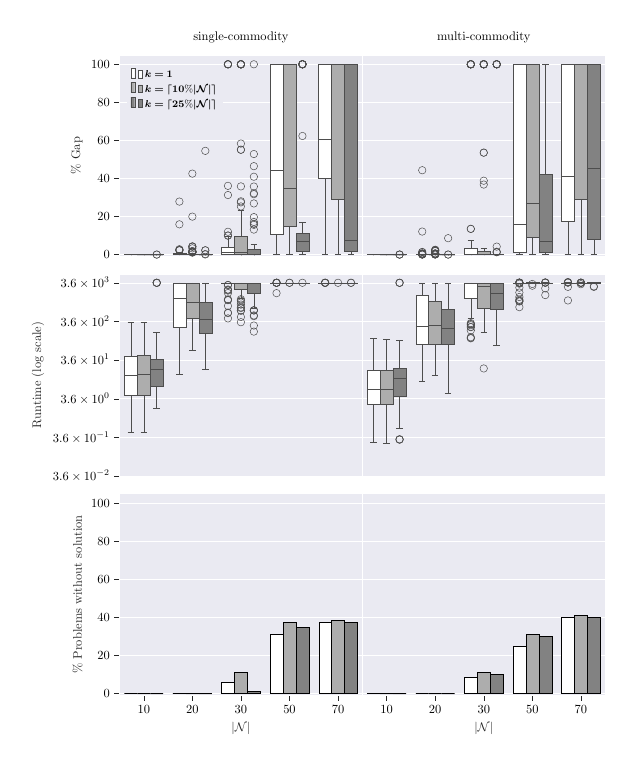
\begin{tikzpicture}[scale=0.45]

\definecolor{darkgray173}{RGB}{173,173,173}
\definecolor{darkslategray38}{RGB}{38,38,38}
\definecolor{darkslategray66}{RGB}{66,66,66}
\definecolor{darkslategray77}{RGB}{77,77,77}
\definecolor{gray130}{RGB}{130,130,130}
\definecolor{lavender234234242}{RGB}{234,234,242}

\begin{groupplot}[group style={group size=2 by 3, vertical sep=0.5cm, horizontal sep=0pt}]
\nextgroupplot[
axis background/.style={fill=lavender234234242},
axis line style={white},
legend cell align={left},
legend style={
  fill opacity=1,
  draw opacity=1,
  text opacity=1,
  font=\footnotesize,
  at={(0.03,0.95)},
  anchor=north west,
  draw=none,
  fill=lavender234234242
},
scaled x ticks=manual:{}{\pgfmathparse{#1}},
tick align=outside,
title={single-commodity},
x grid style={white},
xmajorticks=false,
xmin=-0.5, xmax=4.5,
xtick style={color=darkslategray38},
xticklabels={},
y grid style={white},
ylabel=\textcolor{darkslategray38}{\% Gap},
ymajorgrids,
ymin=-1, ymax=105,
ytick style={color=darkslategray38},
ytick={0,20,40,60,80,100},
yticklabels={
  \(\displaystyle {0}\),
  \(\displaystyle {20}\),
  \(\displaystyle {40}\),
  \(\displaystyle {60}\),
  \(\displaystyle {80}\),
  \(\displaystyle {100}\)
}
]
\addlegendimage{ybar,ybar legend,draw=white!29.8039215686275!black,fill=white,line width=0.3pt}
\addlegendimage{ybar,ybar legend,draw=white!29.8039215686275!black,fill=darkgray173,line width=0.3pt}
\addlegendimage{ybar,ybar legend,draw=white!29.8039215686275!black,fill=gray130,line width=0.3pt}
\addlegendentry{$\bm{k=1}$}
\addlegendentry{$\bm{k=\lceil 10\%|\mathcal N|\rceil}$}
\addlegendentry{$\bm{k=\lceil 25\%|\mathcal N|\rceil}$}
\path [draw=darkslategray77, fill=white]
(axis cs:-0.4,9.88959916819129e-05)
--(axis cs:-0.133333333333333,9.88959916819129e-05)
--(axis cs:-0.133333333333333,0.00591657692962505)
--(axis cs:-0.4,0.00591657692962505)
--(axis cs:-0.4,9.88959916819129e-05)
--cycle;
\addplot [darkslategray77, forget plot]
table {%
-0.266666666666667 9.88959916819129e-05
-0.266666666666667 0
};
\addplot [darkslategray77, forget plot]
table {%
-0.266666666666667 0.00591657692962505
-0.266666666666667 0.00986238748363109
};
\addplot [darkslategray77, forget plot]
table {%
-0.333333333333333 0
-0.2 0
};
\addplot [darkslategray77, forget plot]
table {%
-0.333333333333333 0.00986238748363109
-0.2 0.00986238748363109
};
\path [draw=darkslategray77, fill=white]
(axis cs:0.6,0.00139440421135738)
--(axis cs:0.866666666666667,0.00139440421135738)
--(axis cs:0.866666666666667,0.746184766073172)
--(axis cs:0.6,0.746184766073172)
--(axis cs:0.6,0.00139440421135738)
--cycle;
\addplot [darkslategray77, forget plot]
table {%
0.733333333333333 0.00139440421135738
0.733333333333333 2.40753547211887e-05
};
\addplot [darkslategray77, forget plot]
table {%
0.733333333333333 0.746184766073172
0.733333333333333 1.39540800235063
};
\addplot [darkslategray77, forget plot]
table {%
0.666666666666667 2.40753547211887e-05
0.8 2.40753547211887e-05
};
\addplot [darkslategray77, forget plot]
table {%
0.666666666666667 1.39540800235063
0.8 1.39540800235063
};
\addplot [black, mark=o, mark size=3, mark options={solid,fill opacity=0,draw=darkslategray77}, only marks, forget plot]
table {%
0.733333333333333 2.83799665004793
0.733333333333333 15.9186172784106
0.733333333333333 2.39411320354555
0.733333333333333 2.3717273331677
0.733333333333333 2.37164865736079
0.733333333333333 2.22699430432005
0.733333333333333 27.8573969203345
};
\path [draw=darkslategray77, fill=white]
(axis cs:1.6,0.372239893743445)
--(axis cs:1.86666666666667,0.372239893743445)
--(axis cs:1.86666666666667,4.10161347659665)
--(axis cs:1.6,4.10161347659665)
--(axis cs:1.6,0.372239893743445)
--cycle;
\addplot [darkslategray77, forget plot]
table {%
1.73333333333333 0.372239893743445
1.73333333333333 0.000136160492456225
};
\addplot [darkslategray77, forget plot]
table {%
1.73333333333333 4.10161347659665
1.73333333333333 9.65754333300662
};
\addplot [darkslategray77, forget plot]
table {%
1.66666666666667 0.000136160492456225
1.8 0.000136160492456225
};
\addplot [darkslategray77, forget plot]
table {%
1.66666666666667 9.65754333300662
1.8 9.65754333300662
};
\addplot [black, mark=o, mark size=3, mark options={solid,fill opacity=0,draw=darkslategray77}, only marks, forget plot]
table {%
1.73333333333333 11.9890325401032
1.73333333333333 31.29987005106
1.73333333333333 100
1.73333333333333 9.9166998080027
1.73333333333333 10.0814122414869
1.73333333333333 100
1.73333333333333 100
1.73333333333333 100
1.73333333333333 100
1.73333333333333 36.1317828429306
};
\path [draw=darkslategray77, fill=white]
(axis cs:2.6,10.4625603318024)
--(axis cs:2.86666666666667,10.4625603318024)
--(axis cs:2.86666666666667,100)
--(axis cs:2.6,100)
--(axis cs:2.6,10.4625603318024)
--cycle;
\addplot [darkslategray77, forget plot]
table {%
2.73333333333333 10.4625603318024
2.73333333333333 0.00074350704463909
};
\addplot [darkslategray77, forget plot]
table {%
2.73333333333333 100
2.73333333333333 100
};
\addplot [darkslategray77, forget plot]
table {%
2.66666666666667 0.00074350704463909
2.8 0.00074350704463909
};
\addplot [darkslategray77, forget plot]
table {%
2.66666666666667 100
2.8 100
};
\path [draw=darkslategray77, fill=white]
(axis cs:3.6,40.2468510302977)
--(axis cs:3.86666666666667,40.2468510302977)
--(axis cs:3.86666666666667,100)
--(axis cs:3.6,100)
--(axis cs:3.6,40.2468510302977)
--cycle;
\addplot [darkslategray77, forget plot]
table {%
3.73333333333333 40.2468510302977
3.73333333333333 0.248856019288
};
\addplot [darkslategray77, forget plot]
table {%
3.73333333333333 100
3.73333333333333 100
};
\addplot [darkslategray77, forget plot]
table {%
3.66666666666667 0.248856019288
3.8 0.248856019288
};
\addplot [darkslategray77, forget plot]
table {%
3.66666666666667 100
3.8 100
};
\path [draw=darkslategray77, fill=darkgray173]
(axis cs:-0.133333333333333,0.000114999284851606)
--(axis cs:0.133333333333333,0.000114999284851606)
--(axis cs:0.133333333333333,0.00591657692962505)
--(axis cs:-0.133333333333333,0.00591657692962505)
--(axis cs:-0.133333333333333,0.000114999284851606)
--cycle;
\addplot [darkslategray77, forget plot]
table {%
0 0.000114999284851606
0 0
};
\addplot [darkslategray77, forget plot]
table {%
0 0.00591657692962505
0 0.00986238748363109
};
\addplot [darkslategray77, forget plot]
table {%
-0.0666666666666667 0
0.0666666666666667 0
};
\addplot [darkslategray77, forget plot]
table {%
-0.0666666666666667 0.00986238748363109
0.0666666666666667 0.00986238748363109
};
\path [draw=darkslategray77, fill=darkgray173]
(axis cs:0.866666666666667,0.000897688161694507)
--(axis cs:1.13333333333333,0.000897688161694507)
--(axis cs:1.13333333333333,0.232820190488283)
--(axis cs:0.866666666666667,0.232820190488283)
--(axis cs:0.866666666666667,0.000897688161694507)
--cycle;
\addplot [darkslategray77, forget plot]
table {%
1 0.000897688161694507
1 0
};
\addplot [darkslategray77, forget plot]
table {%
1 0.232820190488283
1 0.56513013609238
};
\addplot [darkslategray77, forget plot]
table {%
0.933333333333333 0
1.06666666666667 0
};
\addplot [darkslategray77, forget plot]
table {%
0.933333333333333 0.56513013609238
1.06666666666667 0.56513013609238
};
\addplot [black, mark=o, mark size=3, mark options={solid,fill opacity=0,draw=darkslategray77}, only marks, forget plot]
table {%
1 1.90909217578163
1 1.6171585193978
1 42.5477051126761
1 19.9498585235363
1 4.10294448576652
1 3.3082368144088
1 1.3578970950807
1 1.3578970950807
1 1.24435283038106
1 1.39920921995736
1 4.30846890205483
1 4.30277114543275
1 1.63478411512995
1 1.37050415595726
1 1.29534349751957
1 1.00407859807943
};
\path [draw=darkslategray77, fill=darkgray173]
(axis cs:1.86666666666667,0.0079437934368307)
--(axis cs:2.13333333333333,0.0079437934368307)
--(axis cs:2.13333333333333,9.47270798899558)
--(axis cs:1.86666666666667,9.47270798899558)
--(axis cs:1.86666666666667,0.0079437934368307)
--cycle;
\addplot [darkslategray77, forget plot]
table {%
2 0.0079437934368307
2 1.67557903244621e-05
};
\addplot [darkslategray77, forget plot]
table {%
2 9.47270798899558
2 23.4357479559391
};
\addplot [darkslategray77, forget plot]
table {%
1.93333333333333 1.67557903244621e-05
2.06666666666667 1.67557903244621e-05
};
\addplot [darkslategray77, forget plot]
table {%
1.93333333333333 23.4357479559391
2.06666666666667 23.4357479559391
};
\addplot [black, mark=o, mark size=3, mark options={solid,fill opacity=0,draw=darkslategray77}, only marks, forget plot]
table {%
2 58.3387306181939
2 100
2 28.0140586931555
2 100
2 55.0909518040008
2 55.0927304097178
2 100
2 35.8462454472341
2 100
2 100
2 100
2 100
2 27.4529522129236
2 25.2965408171533
2 100
};
\path [draw=darkslategray77, fill=darkgray173]
(axis cs:2.86666666666667,14.7183509519659)
--(axis cs:3.13333333333333,14.7183509519659)
--(axis cs:3.13333333333333,100)
--(axis cs:2.86666666666667,100)
--(axis cs:2.86666666666667,14.7183509519659)
--cycle;
\addplot [darkslategray77, forget plot]
table {%
3 14.7183509519659
3 0.12584182964922
};
\addplot [darkslategray77, forget plot]
table {%
3 100
3 100
};
\addplot [darkslategray77, forget plot]
table {%
2.93333333333333 0.12584182964922
3.06666666666667 0.12584182964922
};
\addplot [darkslategray77, forget plot]
table {%
2.93333333333333 100
3.06666666666667 100
};
\path [draw=darkslategray77, fill=darkgray173]
(axis cs:3.86666666666667,29.3165356078277)
--(axis cs:4.13333333333333,29.3165356078277)
--(axis cs:4.13333333333333,100)
--(axis cs:3.86666666666667,100)
--(axis cs:3.86666666666667,29.3165356078277)
--cycle;
\addplot [darkslategray77, forget plot]
table {%
4 29.3165356078277
4 0.37616839818888
};
\addplot [darkslategray77, forget plot]
table {%
4 100
4 100
};
\addplot [darkslategray77, forget plot]
table {%
3.93333333333333 0.37616839818888
4.06666666666667 0.37616839818888
};
\addplot [darkslategray77, forget plot]
table {%
3.93333333333333 100
4.06666666666667 100
};
\path [draw=darkslategray77, fill=gray130]
(axis cs:0.133333333333333,0.00015779650100962)
--(axis cs:0.4,0.00015779650100962)
--(axis cs:0.4,0.00686492658435402)
--(axis cs:0.133333333333333,0.00686492658435402)
--(axis cs:0.133333333333333,0.00015779650100962)
--cycle;
\addplot [darkslategray77, forget plot]
table {%
0.266666666666667 0.00015779650100962
0.266666666666667 0
};
\addplot [darkslategray77, forget plot]
table {%
0.266666666666667 0.00686492658435402
0.266666666666667 0.01647584015881
};
\addplot [darkslategray77, forget plot]
table {%
0.2 0
0.333333333333333 0
};
\addplot [darkslategray77, forget plot]
table {%
0.2 0.01647584015881
0.333333333333333 0.01647584015881
};
\addplot [black, mark=o, mark size=3, mark options={solid,fill opacity=0,draw=darkslategray77}, only marks, forget plot]
table {%
0.266666666666667 0.01716686330995
0.266666666666667 0.02011441348994
};
\path [draw=darkslategray77, fill=gray130]
(axis cs:1.13333333333333,0.000806831484512924)
--(axis cs:1.4,0.000806831484512924)
--(axis cs:1.4,0.00878678714214975)
--(axis cs:1.13333333333333,0.00878678714214975)
--(axis cs:1.13333333333333,0.000806831484512924)
--cycle;
\addplot [darkslategray77, forget plot]
table {%
1.26666666666667 0.000806831484512924
1.26666666666667 0
};
\addplot [darkslategray77, forget plot]
table {%
1.26666666666667 0.00878678714214975
1.26666666666667 0.01533698231403
};
\addplot [darkslategray77, forget plot]
table {%
1.2 0
1.33333333333333 0
};
\addplot [darkslategray77, forget plot]
table {%
1.2 0.01533698231403
1.33333333333333 0.01533698231403
};
\addplot [black, mark=o, mark size=3, mark options={solid,fill opacity=0,draw=darkslategray77}, only marks, forget plot]
table {%
1.26666666666667 54.5096062256846
1.26666666666667 0.31128594034519
1.26666666666667 0.06398391308567
1.26666666666667 2.26902786496918
1.26666666666667 2.26967819952955
};
\path [draw=darkslategray77, fill=gray130]
(axis cs:2.13333333333333,0.00743101723147464)
--(axis cs:2.4,0.00743101723147464)
--(axis cs:2.4,3.02485957515998)
--(axis cs:2.13333333333333,3.02485957515998)
--(axis cs:2.13333333333333,0.00743101723147464)
--cycle;
\addplot [darkslategray77, forget plot]
table {%
2.26666666666667 0.00743101723147464
2.26666666666667 1.73791944892168e-05
};
\addplot [darkslategray77, forget plot]
table {%
2.26666666666667 3.02485957515998
2.26666666666667 5.42564185348612
};
\addplot [darkslategray77, forget plot]
table {%
2.2 1.73791944892168e-05
2.33333333333333 1.73791944892168e-05
};
\addplot [darkslategray77, forget plot]
table {%
2.2 5.42564185348612
2.33333333333333 5.42564185348612
};
\addplot [black, mark=o, mark size=3, mark options={solid,fill opacity=0,draw=darkslategray77}, only marks, forget plot]
table {%
2.26666666666667 15.6159206199839
2.26666666666667 17.1402788560426
2.26666666666667 32.2114077330974
2.26666666666667 31.7427746691043
2.26666666666667 16.1272489208952
2.26666666666667 46.4652765282972
2.26666666666667 40.9101694279538
2.26666666666667 26.8810865527709
2.26666666666667 13.1548688298301
2.26666666666667 19.7119665130021
2.26666666666667 35.7725026017771
2.26666666666667 52.843610049725
2.26666666666667 100
};
\path [draw=darkslategray77, fill=gray130]
(axis cs:3.13333333333333,1.70445221823176)
--(axis cs:3.4,1.70445221823176)
--(axis cs:3.4,11.2099657053925)
--(axis cs:3.13333333333333,11.2099657053925)
--(axis cs:3.13333333333333,1.70445221823176)
--cycle;
\addplot [darkslategray77, forget plot]
table {%
3.26666666666667 1.70445221823176
3.26666666666667 0.15317768824245
};
\addplot [darkslategray77, forget plot]
table {%
3.26666666666667 11.2099657053925
3.26666666666667 16.7589672825689
};
\addplot [darkslategray77, forget plot]
table {%
3.2 0.15317768824245
3.33333333333333 0.15317768824245
};
\addplot [darkslategray77, forget plot]
table {%
3.2 16.7589672825689
3.33333333333333 16.7589672825689
};
\addplot [black, mark=o, mark size=3, mark options={solid,fill opacity=0,draw=darkslategray77}, only marks, forget plot]
table {%
3.26666666666667 100
3.26666666666667 100
3.26666666666667 100
3.26666666666667 100
3.26666666666667 62.325384033416
3.26666666666667 100
3.26666666666667 100
3.26666666666667 100
3.26666666666667 100
3.26666666666667 100
};
\path [draw=darkslategray77, fill=gray130]
(axis cs:4.13333333333333,1.71500246105438)
--(axis cs:4.4,1.71500246105438)
--(axis cs:4.4,100)
--(axis cs:4.13333333333333,100)
--(axis cs:4.13333333333333,1.71500246105438)
--cycle;
\addplot [darkslategray77, forget plot]
table {%
4.26666666666667 1.71500246105438
4.26666666666667 0.41088319841366
};
\addplot [darkslategray77, forget plot]
table {%
4.26666666666667 100
4.26666666666667 100
};
\addplot [darkslategray77, forget plot]
table {%
4.2 0.41088319841366
4.33333333333333 0.41088319841366
};
\addplot [darkslategray77, forget plot]
table {%
4.2 100
4.33333333333333 100
};
\addplot [darkslategray77, forget plot]
table {%
-0.4 0.00170230178119277
-0.133333333333333 0.00170230178119277
};
\addplot [darkslategray77, forget plot]
table {%
0.6 0.00945609702117344
0.866666666666667 0.00945609702117344
};
\addplot [darkslategray77, forget plot]
table {%
1.6 1.35138624951427
1.86666666666667 1.35138624951427
};
\addplot [darkslategray77, forget plot]
table {%
2.6 44.5278992166011
2.86666666666667 44.5278992166011
};
\addplot [darkslategray77, forget plot]
table {%
3.6 60.4116931939782
3.86666666666667 60.4116931939782
};
\addplot [darkslategray77, forget plot]
table {%
-0.133333333333333 0.00170230178119277
0.133333333333333 0.00170230178119277
};
\addplot [darkslategray77, forget plot]
table {%
0.866666666666667 0.00664193155423103
1.13333333333333 0.00664193155423103
};
\addplot [darkslategray77, forget plot]
table {%
1.86666666666667 1.3827801609363
2.13333333333333 1.3827801609363
};
\addplot [darkslategray77, forget plot]
table {%
2.86666666666667 34.989327940183
3.13333333333333 34.989327940183
};
\addplot [darkslategray77, forget plot]
table {%
3.86666666666667 100
4.13333333333333 100
};
\addplot [darkslategray77, forget plot]
table {%
0.133333333333333 0.0015948028477096
0.4 0.0015948028477096
};
\addplot [darkslategray77, forget plot]
table {%
1.13333333333333 0.00518337433946857
1.4 0.00518337433946857
};
\addplot [darkslategray77, forget plot]
table {%
2.13333333333333 0.10223613079794
2.4 0.10223613079794
};
\addplot [darkslategray77, forget plot]
table {%
3.13333333333333 7.22010344381532
3.4 7.22010344381532
};
\addplot [darkslategray77, forget plot]
table {%
4.13333333333333 7.46883195452226
4.4 7.46883195452226
};

\nextgroupplot[
axis background/.style={fill=lavender234234242},
axis line style={white},
scaled x ticks=manual:{}{\pgfmathparse{#1}},
scaled y ticks=manual:{}{\pgfmathparse{#1}},
tick align=outside,
title={multi-commodity},
x grid style={white},
xmajorticks=false,
xmin=-0.5, xmax=4.5,
xtick style={color=darkslategray38},
xticklabels={},
y grid style={white},
ymajorgrids,
ymajorticks=false,
ymin=-1, ymax=105,
ytick style={color=darkslategray38},
yticklabels={}
]
\path [draw=darkslategray77, fill=white]
(axis cs:-0.4,0.000355426360792265)
--(axis cs:-0.133333333333333,0.000355426360792265)
--(axis cs:-0.133333333333333,0.00604550970535129)
--(axis cs:-0.4,0.00604550970535129)
--(axis cs:-0.4,0.000355426360792265)
--cycle;
\addplot [darkslategray77]
table {%
-0.266666666666667 0.000355426360792265
-0.266666666666667 0
};
\addplot [darkslategray77]
table {%
-0.266666666666667 0.00604550970535129
-0.266666666666667 0.00993881385501863
};
\addplot [darkslategray77]
table {%
-0.333333333333333 0
-0.2 0
};
\addplot [darkslategray77]
table {%
-0.333333333333333 0.00993881385501863
-0.2 0.00993881385501863
};
\path [draw=darkslategray77, fill=white]
(axis cs:0.6,0.000495773610963307)
--(axis cs:0.866666666666667,0.000495773610963307)
--(axis cs:0.866666666666667,0.00944099088259695)
--(axis cs:0.6,0.00944099088259695)
--(axis cs:0.6,0.000495773610963307)
--cycle;
\addplot [darkslategray77]
table {%
0.733333333333333 0.000495773610963307
0.733333333333333 3.6778828221793e-06
};
\addplot [darkslategray77]
table {%
0.733333333333333 0.00944099088259695
0.733333333333333 0.02229774445675
};
\addplot [darkslategray77]
table {%
0.666666666666667 3.6778828221793e-06
0.8 3.6778828221793e-06
};
\addplot [darkslategray77]
table {%
0.666666666666667 0.02229774445675
0.8 0.02229774445675
};
\addplot [black, mark=o, mark size=3, mark options={solid,fill opacity=0,draw=darkslategray77}, only marks]
table {%
0.733333333333333 0.61388790345455
0.733333333333333 0.62384437181204
0.733333333333333 1.29757129646422
0.733333333333333 1.37785897890718
0.733333333333333 0.23583848829861
0.733333333333333 12.1129478137183
0.733333333333333 44.3304667808476
0.733333333333333 0.30945342925767
0.733333333333333 0.18530927827884
0.733333333333333 0.26247043734633
0.733333333333333 0.05064328179545
0.733333333333333 0.07468836027385
0.733333333333333 0.03740799805625
0.733333333333333 0.39317800201087
};
\path [draw=darkslategray77, fill=white]
(axis cs:1.6,0.00437855814411925)
--(axis cs:1.86666666666667,0.00437855814411925)
--(axis cs:1.86666666666667,3.36369177194993)
--(axis cs:1.6,3.36369177194993)
--(axis cs:1.6,0.00437855814411925)
--cycle;
\addplot [darkslategray77]
table {%
1.73333333333333 0.00437855814411925
1.73333333333333 1.23694643955478e-08
};
\addplot [darkslategray77]
table {%
1.73333333333333 3.36369177194993
1.73333333333333 7.65908293477156
};
\addplot [darkslategray77]
table {%
1.66666666666667 1.23694643955478e-08
1.8 1.23694643955478e-08
};
\addplot [darkslategray77]
table {%
1.66666666666667 7.65908293477156
1.8 7.65908293477156
};
\addplot [black, mark=o, mark size=3, mark options={solid,fill opacity=0,draw=darkslategray77}, only marks]
table {%
1.73333333333333 100
1.73333333333333 100
1.73333333333333 100
1.73333333333333 100
1.73333333333333 100
1.73333333333333 13.5254016361461
1.73333333333333 13.5254016361461
1.73333333333333 100
1.73333333333333 100
1.73333333333333 100
};
\path [draw=darkslategray77, fill=white]
(axis cs:2.6,1.02888945230666)
--(axis cs:2.86666666666667,1.02888945230666)
--(axis cs:2.86666666666667,100)
--(axis cs:2.6,100)
--(axis cs:2.6,1.02888945230666)
--cycle;
\addplot [darkslategray77]
table {%
2.73333333333333 1.02888945230666
2.73333333333333 4.00654585343835e-05
};
\addplot [darkslategray77]
table {%
2.73333333333333 100
2.73333333333333 100
};
\addplot [darkslategray77]
table {%
2.66666666666667 4.00654585343835e-05
2.8 4.00654585343835e-05
};
\addplot [darkslategray77]
table {%
2.66666666666667 100
2.8 100
};
\path [draw=darkslategray77, fill=white]
(axis cs:3.6,17.7033171077893)
--(axis cs:3.86666666666667,17.7033171077893)
--(axis cs:3.86666666666667,100)
--(axis cs:3.6,100)
--(axis cs:3.6,17.7033171077893)
--cycle;
\addplot [darkslategray77]
table {%
3.73333333333333 17.7033171077893
3.73333333333333 0.000638959375493919
};
\addplot [darkslategray77]
table {%
3.73333333333333 100
3.73333333333333 100
};
\addplot [darkslategray77]
table {%
3.66666666666667 0.000638959375493919
3.8 0.000638959375493919
};
\addplot [darkslategray77]
table {%
3.66666666666667 100
3.8 100
};
\path [draw=darkslategray77, fill=darkgray173]
(axis cs:-0.133333333333333,0.000571027242322059)
--(axis cs:0.133333333333333,0.000571027242322059)
--(axis cs:0.133333333333333,0.0065570891713595)
--(axis cs:-0.133333333333333,0.0065570891713595)
--(axis cs:-0.133333333333333,0.000571027242322059)
--cycle;
\addplot [darkslategray77]
table {%
0 0.000571027242322059
0 0
};
\addplot [darkslategray77]
table {%
0 0.0065570891713595
0 0.00986218438239089
};
\addplot [darkslategray77]
table {%
-0.0666666666666667 0
0.0666666666666667 0
};
\addplot [darkslategray77]
table {%
-0.0666666666666667 0.00986218438239089
0.0666666666666667 0.00986218438239089
};
\path [draw=darkslategray77, fill=darkgray173]
(axis cs:0.866666666666667,0.000677733810831334)
--(axis cs:1.13333333333333,0.000677733810831334)
--(axis cs:1.13333333333333,0.00980152423486129)
--(axis cs:0.866666666666667,0.00980152423486129)
--(axis cs:0.866666666666667,0.000677733810831334)
--cycle;
\addplot [darkslategray77]
table {%
1 0.000677733810831334
1 0
};
\addplot [darkslategray77]
table {%
1 0.00980152423486129
1 0.0180973011568
};
\addplot [darkslategray77]
table {%
0.933333333333333 0
1.06666666666667 0
};
\addplot [darkslategray77]
table {%
0.933333333333333 0.0180973011568
1.06666666666667 0.0180973011568
};
\addplot [black, mark=o, mark size=3, mark options={solid,fill opacity=0,draw=darkslategray77}, only marks]
table {%
1 1.91938548962605
1 1.91938548962605
1 2.34491626469436
1 2.56029347961817
1 0.52348045158277
1 0.62805717715904
1 1.96255133639009
1 2.35062797140051
1 0.09432578364893
1 0.14930669918111
1 0.53387621696224
1 0.39679228038132
1 0.37572560617582
1 0.39094093914639
1 0.09435639153841
1 0.06133529349032
};
\path [draw=darkslategray77, fill=darkgray173]
(axis cs:1.86666666666667,0.00194190694994986)
--(axis cs:2.13333333333333,0.00194190694994986)
--(axis cs:2.13333333333333,1.55168517709577)
--(axis cs:1.86666666666667,1.55168517709577)
--(axis cs:1.86666666666667,0.00194190694994986)
--cycle;
\addplot [darkslategray77]
table {%
2 0.00194190694994986
2 6.57325091893148e-06
};
\addplot [darkslategray77]
table {%
2 1.55168517709577
2 3.12081731261197
};
\addplot [darkslategray77]
table {%
1.93333333333333 6.57325091893148e-06
2.06666666666667 6.57325091893148e-06
};
\addplot [darkslategray77]
table {%
1.93333333333333 3.12081731261197
2.06666666666667 3.12081731261197
};
\addplot [black, mark=o, mark size=3, mark options={solid,fill opacity=0,draw=darkslategray77}, only marks]
table {%
2 100
2 36.8059943370725
2 38.8144064441509
2 100
2 53.5661945854495
2 53.5660174944889
2 100
2 100
2 100
2 100
2 100
2 100
};
\path [draw=darkslategray77, fill=darkgray173]
(axis cs:2.86666666666667,9.00982212820727)
--(axis cs:3.13333333333333,9.00982212820727)
--(axis cs:3.13333333333333,100)
--(axis cs:2.86666666666667,100)
--(axis cs:2.86666666666667,9.00982212820727)
--cycle;
\addplot [darkslategray77]
table {%
3 9.00982212820727
3 0.000475876986721706
};
\addplot [darkslategray77]
table {%
3 100
3 100
};
\addplot [darkslategray77]
table {%
2.93333333333333 0.000475876986721706
3.06666666666667 0.000475876986721706
};
\addplot [darkslategray77]
table {%
2.93333333333333 100
3.06666666666667 100
};
\path [draw=darkslategray77, fill=darkgray173]
(axis cs:3.86666666666667,28.9520095794459)
--(axis cs:4.13333333333333,28.9520095794459)
--(axis cs:4.13333333333333,100)
--(axis cs:3.86666666666667,100)
--(axis cs:3.86666666666667,28.9520095794459)
--cycle;
\addplot [darkslategray77]
table {%
4 28.9520095794459
4 0.0061341555230636
};
\addplot [darkslategray77]
table {%
4 100
4 100
};
\addplot [darkslategray77]
table {%
3.93333333333333 0.0061341555230636
4.06666666666667 0.0061341555230636
};
\addplot [darkslategray77]
table {%
3.93333333333333 100
4.06666666666667 100
};
\path [draw=darkslategray77, fill=gray130]
(axis cs:0.133333333333333,0.000367454774025498)
--(axis cs:0.4,0.000367454774025498)
--(axis cs:0.4,0.00577174549653221)
--(axis cs:0.133333333333333,0.00577174549653221)
--(axis cs:0.133333333333333,0.000367454774025498)
--cycle;
\addplot [darkslategray77]
table {%
0.266666666666667 0.000367454774025498
0.266666666666667 0
};
\addplot [darkslategray77]
table {%
0.266666666666667 0.00577174549653221
0.266666666666667 0.00943206025384057
};
\addplot [darkslategray77]
table {%
0.2 0
0.333333333333333 0
};
\addplot [darkslategray77]
table {%
0.2 0.00943206025384057
0.333333333333333 0.00943206025384057
};
\addplot [black, mark=o, mark size=3, mark options={solid,fill opacity=0,draw=darkslategray77}, only marks]
table {%
0.266666666666667 0.01590952346553
0.266666666666667 0.01413024739351
0.266666666666667 0.01799198308724
};
\path [draw=darkslategray77, fill=gray130]
(axis cs:1.13333333333333,0.00147483682579351)
--(axis cs:1.4,0.00147483682579351)
--(axis cs:1.4,0.00850668948469766)
--(axis cs:1.13333333333333,0.00850668948469766)
--(axis cs:1.13333333333333,0.00147483682579351)
--cycle;
\addplot [darkslategray77]
table {%
1.26666666666667 0.00147483682579351
1.26666666666667 0
};
\addplot [darkslategray77]
table {%
1.26666666666667 0.00850668948469766
1.26666666666667 0.01660940312298
};
\addplot [darkslategray77]
table {%
1.2 0
1.33333333333333 0
};
\addplot [darkslategray77]
table {%
1.2 0.01660940312298
1.33333333333333 0.01660940312298
};
\addplot [black, mark=o, mark size=3, mark options={solid,fill opacity=0,draw=darkslategray77}, only marks]
table {%
1.26666666666667 8.62113243239045
1.26666666666667 0.0199753180264
1.26666666666667 0.02255172444655
};
\path [draw=darkslategray77, fill=gray130]
(axis cs:2.13333333333333,0.00559086831044699)
--(axis cs:2.4,0.00559086831044699)
--(axis cs:2.4,0.150846933677557)
--(axis cs:2.13333333333333,0.150846933677557)
--(axis cs:2.13333333333333,0.00559086831044699)
--cycle;
\addplot [darkslategray77]
table {%
2.26666666666667 0.00559086831044699
2.26666666666667 4.57187053933903e-06
};
\addplot [darkslategray77]
table {%
2.26666666666667 0.150846933677557
2.26666666666667 0.31236388018016
};
\addplot [darkslategray77]
table {%
2.2 4.57187053933903e-06
2.33333333333333 4.57187053933903e-06
};
\addplot [darkslategray77]
table {%
2.2 0.31236388018016
2.33333333333333 0.31236388018016
};
\addplot [black, mark=o, mark size=3, mark options={solid,fill opacity=0,draw=darkslategray77}, only marks]
table {%
2.26666666666667 4.19890355853189
2.26666666666667 100
2.26666666666667 1.51143637218262
2.26666666666667 100
2.26666666666667 100
2.26666666666667 100
2.26666666666667 100
2.26666666666667 100
2.26666666666667 1.28736985216044
2.26666666666667 1.25983011206012
2.26666666666667 100
};
\path [draw=darkslategray77, fill=gray130]
(axis cs:3.13333333333333,1.43772343895019)
--(axis cs:3.4,1.43772343895019)
--(axis cs:3.4,42.155290083801)
--(axis cs:3.13333333333333,42.155290083801)
--(axis cs:3.13333333333333,1.43772343895019)
--cycle;
\addplot [darkslategray77]
table {%
3.26666666666667 1.43772343895019
3.26666666666667 0.00487254517973941
};
\addplot [darkslategray77]
table {%
3.26666666666667 42.155290083801
3.26666666666667 100
};
\addplot [darkslategray77]
table {%
3.2 0.00487254517973941
3.33333333333333 0.00487254517973941
};
\addplot [darkslategray77]
table {%
3.2 100
3.33333333333333 100
};
\path [draw=darkslategray77, fill=gray130]
(axis cs:4.13333333333333,8.03636523563109)
--(axis cs:4.4,8.03636523563109)
--(axis cs:4.4,100)
--(axis cs:4.13333333333333,100)
--(axis cs:4.13333333333333,8.03636523563109)
--cycle;
\addplot [darkslategray77]
table {%
4.26666666666667 8.03636523563109
4.26666666666667 0.0031199611077771
};
\addplot [darkslategray77]
table {%
4.26666666666667 100
4.26666666666667 100
};
\addplot [darkslategray77]
table {%
4.2 0.0031199611077771
4.33333333333333 0.0031199611077771
};
\addplot [darkslategray77]
table {%
4.2 100
4.33333333333333 100
};
\addplot [darkslategray77]
table {%
-0.4 0.00267458036476814
-0.133333333333333 0.00267458036476814
};
\addplot [darkslategray77]
table {%
0.6 0.00660826419245593
0.866666666666667 0.00660826419245593
};
\addplot [darkslategray77]
table {%
1.6 0.18772503679995
1.86666666666667 0.18772503679995
};
\addplot [darkslategray77]
table {%
2.6 15.9318439793709
2.86666666666667 15.9318439793709
};
\addplot [darkslategray77]
table {%
3.6 41.4203741441358
3.86666666666667 41.4203741441358
};
\addplot [darkslategray77]
table {%
-0.133333333333333 0.00298425811177514
0.133333333333333 0.00298425811177514
};
\addplot [darkslategray77]
table {%
0.866666666666667 0.00570354052470974
1.13333333333333 0.00570354052470974
};
\addplot [darkslategray77]
table {%
1.86666666666667 0.00990044372115028
2.13333333333333 0.00990044372115028
};
\addplot [darkslategray77]
table {%
2.86666666666667 26.9852998076058
3.13333333333333 26.9852998076058
};
\addplot [darkslategray77]
table {%
3.86666666666667 100
4.13333333333333 100
};
\addplot [darkslategray77]
table {%
0.133333333333333 0.00238206442473166
0.4 0.00238206442473166
};
\addplot [darkslategray77]
table {%
1.13333333333333 0.0058161743819604
1.4 0.0058161743819604
};
\addplot [darkslategray77]
table {%
2.13333333333333 0.00941072920122985
2.4 0.00941072920122985
};
\addplot [darkslategray77]
table {%
3.13333333333333 7.04715201141966
3.4 7.04715201141966
};
\addplot [darkslategray77]
table {%
4.13333333333333 45.4699019129198
4.4 45.4699019129198
};

\nextgroupplot[
axis background/.style={fill=lavender234234242},
axis line style={white},
log basis y={10},
scaled x ticks=manual:{}{\pgfmathparse{#1}},
scaled y ticks=manual:{}{\pgfmathparse{#1}},
tick align=outside,
x grid style={white},
xmajorticks=false,
xmin=-0.5, xmax=4.5,
xtick style={color=darkslategray38},
xticklabels={},
y grid style={white},
ylabel=\textcolor{darkslategray38}{Runtime (log scale)},
ymajorgrids,
ymajorticks,
ymin=0.036, ymax=6000,
ymode=log,
ytick style={color=darkslategray38},
ytick={0.036,0.36,3.6,36,360,3600},
yticklabels={
  \(\displaystyle 3.6\times 10^{-2}\),
  \(\displaystyle 3.6\times 10^{-1}\),
  \(\displaystyle 3.6\times 10^{0}\),
  \(\displaystyle 3.6\times 10^{1}\),
  \(\displaystyle 3.6\times 10^{2}\),
  \(\displaystyle 3.6\times 10^{3}\)
}
]
\path [draw=darkslategray77, fill=white]
(axis cs:-0.4,4.3109562652889)
--(axis cs:-0.133333333333333,4.3109562652889)
--(axis cs:-0.133333333333333,46.0540453903309)
--(axis cs:-0.4,46.0540453903309)
--(axis cs:-0.4,4.3109562652889)
--cycle;
\addplot [darkslategray77]
table {%
-0.266666666666667 4.3109562652889
-0.266666666666667 0.473899841308594
};
\addplot [darkslategray77]
table {%
-0.266666666666667 46.0540453903309
-0.266666666666667 339.079997777939
};
\addplot [darkslategray77]
table {%
-0.333333333333333 0.473899841308594
-0.2 0.473899841308594
};
\addplot [darkslategray77]
table {%
-0.333333333333333 339.079997777939
-0.2 339.079997777939
};
\path [draw=darkslategray77, fill=white]
(axis cs:0.6,256.241873677136)
--(axis cs:0.866666666666667,256.241873677136)
--(axis cs:0.866666666666667,3600.16391092539)
--(axis cs:0.6,3600.16391092539)
--(axis cs:0.6,256.241873677136)
--cycle;
\addplot [darkslategray77]
table {%
0.733333333333333 256.241873677136
0.733333333333333 15.6860361099243
};
\addplot [darkslategray77]
table {%
0.733333333333333 3600.16391092539
0.733333333333333 3600.70693778992
};
\addplot [darkslategray77]
table {%
0.666666666666667 15.6860361099243
0.8 15.6860361099243
};
\addplot [darkslategray77]
table {%
0.666666666666667 3600.70693778992
0.8 3600.70693778992
};
\path [draw=darkslategray77, fill=white]
(axis cs:1.6,3600.11677443488)
--(axis cs:1.86666666666667,3600.11677443488)
--(axis cs:1.86666666666667,3600.4813222247)
--(axis cs:1.6,3600.4813222247)
--(axis cs:1.6,3600.11677443488)
--cycle;
\addplot [darkslategray77]
table {%
1.73333333333333 3600.11677443488
1.73333333333333 3600.09260702133
};
\addplot [darkslategray77]
table {%
1.73333333333333 3600.4813222247
1.73333333333333 3600.70876598358
};
\addplot [darkslategray77]
table {%
1.66666666666667 3600.09260702133
1.8 3600.09260702133
};
\addplot [darkslategray77]
table {%
1.66666666666667 3600.70876598358
1.8 3600.70876598358
};
\addplot [black, mark=o, mark size=3, mark options={solid,fill opacity=0,draw=darkslategray77}, only marks]
table {%
1.73333333333333 590.63399720192
1.73333333333333 607.867830038071
1.73333333333333 906.655798912048
1.73333333333333 1957.65879511833
1.73333333333333 2416.79896116257
1.73333333333333 2349.10485386848
1.73333333333333 2262.20754408836
1.73333333333333 1296.54971694946
1.73333333333333 1276.19936203957
1.73333333333333 3158.4145488739
1.73333333333333 3154.87415504456
1.73333333333333 1343.99403595924
1.73333333333333 431.571033000946
};
\path [draw=darkslategray77, fill=white]
(axis cs:2.6,3600.23929500383)
--(axis cs:2.86666666666667,3600.23929500383)
--(axis cs:2.86666666666667,3600.52152988528)
--(axis cs:2.6,3600.52152988528)
--(axis cs:2.6,3600.23929500383)
--cycle;
\addplot [darkslategray77]
table {%
2.73333333333333 3600.23929500383
2.73333333333333 3600.09494209289
};
\addplot [darkslategray77]
table {%
2.73333333333333 3600.52152988528
2.73333333333333 3600.61145114898
};
\addplot [darkslategray77]
table {%
2.66666666666667 3600.09494209289
2.8 3600.09494209289
};
\addplot [darkslategray77]
table {%
2.66666666666667 3600.61145114898
2.8 3600.61145114898
};
\addplot [black, mark=o, mark size=3, mark options={solid,fill opacity=0,draw=darkslategray77}, only marks]
table {%
2.73333333333333 1945.18206906319
2.73333333333333 3602.1657140255
2.73333333333333 3602.01010799408
2.73333333333333 3601.49046778679
2.73333333333333 3601.45016503334
2.73333333333333 3601.54521393776
2.73333333333333 3601.45844292641
};
\path [draw=darkslategray77, fill=white]
(axis cs:3.6,3600.35325987432)
--(axis cs:3.86666666666667,3600.35325987432)
--(axis cs:3.86666666666667,3600.76990443311)
--(axis cs:3.6,3600.76990443311)
--(axis cs:3.6,3600.35325987432)
--cycle;
\addplot [darkslategray77]
table {%
3.73333333333333 3600.35325987432
3.73333333333333 3600.10244584084
};
\addplot [darkslategray77]
table {%
3.73333333333333 3600.76990443311
3.73333333333333 3600.8378059864
};
\addplot [darkslategray77]
table {%
3.66666666666667 3600.10244584084
3.8 3600.10244584084
};
\addplot [darkslategray77]
table {%
3.66666666666667 3600.8378059864
3.8 3600.8378059864
};
\addplot [black, mark=o, mark size=3, mark options={solid,fill opacity=0,draw=darkslategray77}, only marks]
table {%
3.73333333333333 3601.64351320267
3.73333333333333 3602.11490511894
3.73333333333333 3602.00066804886
3.73333333333333 3602.1009991169
3.73333333333333 3602.09011697769
};
\path [draw=darkslategray77, fill=darkgray173]
(axis cs:-0.133333333333333,4.35667043307947)
--(axis cs:0.133333333333333,4.35667043307947)
--(axis cs:0.133333333333333,46.7455162701073)
--(axis cs:-0.133333333333333,46.7455162701073)
--(axis cs:-0.133333333333333,4.35667043307947)
--cycle;
\addplot [darkslategray77]
table {%
0 4.35667043307947
0 0.477431058883667
};
\addplot [darkslategray77]
table {%
0 46.7455162701073
0 340.912337779999
};
\addplot [darkslategray77]
table {%
-0.0666666666666667 0.477431058883667
0.0666666666666667 0.477431058883667
};
\addplot [darkslategray77]
table {%
-0.0666666666666667 340.912337779999
0.0666666666666667 340.912337779999
};
\path [draw=darkslategray77, fill=darkgray173]
(axis cs:0.866666666666667,424.53922213512)
--(axis cs:1.13333333333333,424.53922213512)
--(axis cs:1.13333333333333,3600.14991003076)
--(axis cs:0.866666666666667,3600.14991003076)
--(axis cs:0.866666666666667,424.53922213512)
--cycle;
\addplot [darkslategray77]
table {%
1 424.53922213512
1 63.0038979053497
};
\addplot [darkslategray77]
table {%
1 3600.14991003076
1 3600.44098496437
};
\addplot [darkslategray77]
table {%
0.933333333333333 63.0038979053497
1.06666666666667 63.0038979053497
};
\addplot [darkslategray77]
table {%
0.933333333333333 3600.44098496437
1.06666666666667 3600.44098496437
};
\path [draw=darkslategray77, fill=darkgray173]
(axis cs:1.86666666666667,2475.91050376857)
--(axis cs:2.13333333333333,2475.91050376857)
--(axis cs:2.13333333333333,3600.27614843675)
--(axis cs:1.86666666666667,3600.27614843675)
--(axis cs:1.86666666666667,2475.91050376857)
--cycle;
\addplot [darkslategray77]
table {%
2 2475.91050376857
2 1433.63995909691
};
\addplot [darkslategray77]
table {%
2 3600.27614843675
2 3600.79825806618
};
\addplot [darkslategray77]
table {%
1.93333333333333 1433.63995909691
2.06666666666667 1433.63995909691
};
\addplot [darkslategray77]
table {%
1.93333333333333 3600.79825806618
2.06666666666667 3600.79825806618
};
\addplot [black, mark=o, mark size=3, mark options={solid,fill opacity=0,draw=darkslategray77}, only marks]
table {%
2 1256.78013300896
2 686.402755022049
2 685.237431049347
2 1112.83164596558
2 468.972458839417
2 343.803662061691
2 831.938564062119
2 1354.34141802788
2 798.469398975372
2 981.23017001152
};
\path [draw=darkslategray77, fill=darkgray173]
(axis cs:2.86666666666667,3600.1721060276)
--(axis cs:3.13333333333333,3600.1721060276)
--(axis cs:3.13333333333333,3600.30946493149)
--(axis cs:2.86666666666667,3600.30946493149)
--(axis cs:2.86666666666667,3600.1721060276)
--cycle;
\addplot [darkslategray77]
table {%
3 3600.1721060276
3 3600.03791594505
};
\addplot [darkslategray77]
table {%
3 3600.30946493149
3 3600.5110309124
};
\addplot [darkslategray77]
table {%
2.93333333333333 3600.03791594505
3.06666666666667 3600.03791594505
};
\addplot [darkslategray77]
table {%
2.93333333333333 3600.5110309124
3.06666666666667 3600.5110309124
};
\addplot [black, mark=o, mark size=3, mark options={solid,fill opacity=0,draw=darkslategray77}, only marks]
table {%
3 3600.55458402634
3 3600.66347002983
};
\path [draw=darkslategray77, fill=darkgray173]
(axis cs:3.86666666666667,3600.32352220985)
--(axis cs:4.13333333333333,3600.32352220985)
--(axis cs:4.13333333333333,3600.64464177323)
--(axis cs:3.86666666666667,3600.64464177323)
--(axis cs:3.86666666666667,3600.32352220985)
--cycle;
\addplot [darkslategray77]
table {%
4 3600.32352220985
4 3600.13685297966
};
\addplot [darkslategray77]
table {%
4 3600.64464177323
4 3601.03802800179
};
\addplot [darkslategray77]
table {%
3.93333333333333 3600.13685297966
4.06666666666667 3600.13685297966
};
\addplot [darkslategray77]
table {%
3.93333333333333 3601.03802800179
4.06666666666667 3601.03802800179
};
\addplot [black, mark=o, mark size=3, mark options={solid,fill opacity=0,draw=darkslategray77}, only marks]
table {%
4 3601.6182858944
};
\path [draw=darkslategray77, fill=gray130]
(axis cs:0.133333333333333,7.55961712146961)
--(axis cs:0.4,7.55961712146961)
--(axis cs:0.4,36.9527538071955)
--(axis cs:0.133333333333333,36.9527538071955)
--(axis cs:0.133333333333333,7.55961712146961)
--cycle;
\addplot [darkslategray77]
table {%
0.266666666666667 7.55961712146961
0.266666666666667 2.07562613487244
};
\addplot [darkslategray77]
table {%
0.266666666666667 36.9527538071955
0.266666666666667 186.300193071365
};
\addplot [darkslategray77]
table {%
0.2 2.07562613487244
0.333333333333333 2.07562613487244
};
\addplot [darkslategray77]
table {%
0.2 186.300193071365
0.333333333333333 186.300193071365
};
\addplot [black, mark=o, mark size=3, mark options={solid,fill opacity=0,draw=darkslategray77}, only marks]
table {%
0.266666666666667 3600.01144719124
0.266666666666667 3600.01951599121
0.266666666666667 3600.02227306366
0.266666666666667 3600.0270459652
};
\path [draw=darkslategray77, fill=gray130]
(axis cs:1.13333333333333,182.550731326098)
--(axis cs:1.4,182.550731326098)
--(axis cs:1.4,1112.30256740369)
--(axis cs:1.13333333333333,1112.30256740369)
--(axis cs:1.13333333333333,182.550731326098)
--cycle;
\addplot [darkslategray77]
table {%
1.26666666666667 182.550731326098
1.26666666666667 20.7725141048431
};
\addplot [darkslategray77]
table {%
1.26666666666667 1112.30256740369
1.26666666666667 3600.31461501122
};
\addplot [darkslategray77]
table {%
1.2 20.7725141048431
1.33333333333333 20.7725141048431
};
\addplot [darkslategray77]
table {%
1.2 3600.31461501122
1.33333333333333 3600.31461501122
};
\path [draw=darkslategray77, fill=gray130]
(axis cs:2.13333333333333,1895.92634403218)
--(axis cs:2.4,1895.92634403218)
--(axis cs:2.4,3600.43664539347)
--(axis cs:2.13333333333333,3600.43664539347)
--(axis cs:2.13333333333333,1895.92634403218)
--cycle;
\addplot [darkslategray77]
table {%
2.26666666666667 1895.92634403218
2.26666666666667 771.999285936355
};
\addplot [darkslategray77]
table {%
2.26666666666667 3600.43664539347
2.26666666666667 3600.69135212898
};
\addplot [darkslategray77]
table {%
2.2 771.999285936355
2.33333333333333 771.999285936355
};
\addplot [darkslategray77]
table {%
2.2 3600.69135212898
2.33333333333333 3600.69135212898
};
\addplot [black, mark=o, mark size=3, mark options={solid,fill opacity=0,draw=darkslategray77}, only marks]
table {%
2.26666666666667 699.784878015519
2.26666666666667 282.105642080307
2.26666666666667 196.345447063446
2.26666666666667 695.234676837921
2.26666666666667 493.595369815826
2.26666666666667 515.556846141815
2.26666666666667 693.370111942291
};
\path [draw=darkslategray77, fill=gray130]
(axis cs:3.13333333333333,3600.30237042623)
--(axis cs:3.4,3600.30237042623)
--(axis cs:3.4,3600.94891731601)
--(axis cs:3.13333333333333,3600.94891731601)
--(axis cs:3.13333333333333,3600.30237042623)
--cycle;
\addplot [darkslategray77]
table {%
3.26666666666667 3600.30237042623
3.26666666666667 3600.05893087387
};
\addplot [darkslategray77]
table {%
3.26666666666667 3600.94891731601
3.26666666666667 3601.67202591896
};
\addplot [darkslategray77]
table {%
3.2 3600.05893087387
3.33333333333333 3600.05893087387
};
\addplot [darkslategray77]
table {%
3.2 3601.67202591896
3.33333333333333 3601.67202591896
};
\addplot [black, mark=o, mark size=3, mark options={solid,fill opacity=0,draw=darkslategray77}, only marks]
table {%
3.26666666666667 3602.0576851368
};
\path [draw=darkslategray77, fill=gray130]
(axis cs:4.13333333333333,3600.30634814495)
--(axis cs:4.4,3600.30634814495)
--(axis cs:4.4,3600.82747447446)
--(axis cs:4.13333333333333,3600.82747447446)
--(axis cs:4.13333333333333,3600.30634814495)
--cycle;
\addplot [darkslategray77]
table {%
4.26666666666667 3600.30634814495
4.26666666666667 3600.25183296204
};
\addplot [darkslategray77]
table {%
4.26666666666667 3600.82747447446
4.26666666666667 3601.09951591492
};
\addplot [darkslategray77]
table {%
4.2 3600.25183296204
4.33333333333333 3600.25183296204
};
\addplot [darkslategray77]
table {%
4.2 3601.09951591492
4.33333333333333 3601.09951591492
};
\addplot [black, mark=o, mark size=3, mark options={solid,fill opacity=0,draw=darkslategray77}, only marks]
table {%
4.26666666666667 3602.36336708069
4.26666666666667 3602.28519511223
};
\addplot [darkslategray77]
table {%
-0.4 14.823968462706
-0.133333333333333 14.823968462706
};
\addplot [darkslategray77]
table {%
0.6 1444.41928184989
0.866666666666667 1444.41928184989
};
\addplot [darkslategray77]
table {%
1.6 3600.22805750355
1.86666666666667 3600.22805750355
};
\addplot [darkslategray77]
table {%
2.6 3600.36385393143
2.86666666666667 3600.36385393143
};
\addplot [darkslategray77]
table {%
3.6 3600.50498604774
3.86666666666667 3600.50498604774
};
\addplot [darkslategray77]
table {%
-0.133333333333333 15.5466862971385
0.133333333333333 15.5466862971385
};
\addplot [darkslategray77]
table {%
0.866666666666667 1097.35439329781
1.13333333333333 1097.35439329781
};
\addplot [darkslategray77]
table {%
1.86666666666667 3600.15846681595
2.13333333333333 3600.15846681595
};
\addplot [darkslategray77]
table {%
2.86666666666667 3600.24076199532
3.13333333333333 3600.24076199532
};
\addplot [darkslategray77]
table {%
3.86666666666667 3600.37334292607
4.13333333333333 3600.37334292607
};
\addplot [darkslategray77]
table {%
0.133333333333333 20.2786651992924
0.4 20.2786651992924
};
\addplot [darkslategray77]
table {%
1.13333333333333 420.694499538328
1.4 420.694499538328
};
\addplot [darkslategray77]
table {%
2.13333333333333 3600.20821402673
2.4 3600.20821402673
};
\addplot [darkslategray77]
table {%
3.13333333333333 3600.41256213188
3.4 3600.41256213188
};
\addplot [darkslategray77]
table {%
4.13333333333333 3600.54432198467
4.4 3600.54432198467
};

\nextgroupplot[
axis background/.style={fill=lavender234234242},
axis line style={white},
log basis y={10},
scaled x ticks=manual:{}{\pgfmathparse{#1}},
tick align=outside,
x grid style={white},
xmin=-0.5, xmax=4.5,
xmajorticks=false,
xtick style={color=darkslategray38},
xticklabels={},
y grid style={white},
ymajorgrids,
ymode=log,
ymajorticks=false,
ymin=0.036, ymax=6000,
ytick={0.036,0.36,3.6,36,360,3600},
yticklabels={}
]
\path [draw=darkslategray77, fill=white]
(axis cs:-0.4,2.59249667993728)
--(axis cs:-0.133333333333333,2.59249667993728)
--(axis cs:-0.133333333333333,19.665529626668)
--(axis cs:-0.4,19.665529626668)
--(axis cs:-0.4,2.59249667993728)
--cycle;
\addplot [darkslategray77]
table {%
-0.266666666666667 2.59249667993728
-0.266666666666667 0.260791063308716
};
\addplot [darkslategray77]
table {%
-0.266666666666667 19.665529626668
-0.266666666666667 130.226570129395
};
\addplot [darkslategray77]
table {%
-0.333333333333333 0.260791063308716
-0.2 0.260791063308716
};
\addplot [darkslategray77]
table {%
-0.333333333333333 130.226570129395
-0.2 130.226570129395
};
\path [draw=darkslategray77, fill=white]
(axis cs:0.6,91.4426612987471)
--(axis cs:0.866666666666667,91.4426612987471)
--(axis cs:0.866666666666667,1759.969452473)
--(axis cs:0.6,1759.969452473)
--(axis cs:0.6,91.4426612987471)
--cycle;
\addplot [darkslategray77]
table {%
0.733333333333333 91.4426612987471
0.733333333333333 9.92947506904602
};
\addplot [darkslategray77]
table {%
0.733333333333333 1759.969452473
0.733333333333333 3601.47388005257
};
\addplot [darkslategray77]
table {%
0.666666666666667 9.92947506904602
0.8 9.92947506904602
};
\addplot [darkslategray77]
table {%
0.666666666666667 3601.47388005257
0.8 3601.47388005257
};
\path [draw=darkslategray77, fill=white]
(axis cs:1.6,1429.78417897225)
--(axis cs:1.86666666666667,1429.78417897225)
--(axis cs:1.86666666666667,3602.10101318359)
--(axis cs:1.6,3602.10101318359)
--(axis cs:1.6,1429.78417897225)
--cycle;
\addplot [darkslategray77]
table {%
1.73333333333333 1429.78417897225
1.73333333333333 423.807388067245
};
\addplot [darkslategray77]
table {%
1.73333333333333 3602.10101318359
1.73333333333333 3608.29213500023
};
\addplot [darkslategray77]
table {%
1.66666666666667 423.807388067245
1.8 423.807388067245
};
\addplot [darkslategray77]
table {%
1.66666666666667 3608.29213500023
1.8 3608.29213500023
};
\addplot [black, mark=o, mark size=3, mark options={solid,fill opacity=0,draw=darkslategray77}, only marks]
table {%
1.73333333333333 255.300072908402
1.73333333333333 259.556859016419
1.73333333333333 286.789654970169
1.73333333333333 211.064751148224
1.73333333333333 140.369524002075
1.73333333333333 324.813682079315
1.73333333333333 134.694375038147
1.73333333333333 131.798241853714
1.73333333333333 303.693960905075
1.73333333333333 308.628530025482
};
\path [draw=darkslategray77, fill=white]
(axis cs:2.6,3600.14727364706)
--(axis cs:2.86666666666667,3600.14727364706)
--(axis cs:2.86666666666667,3603.5343929655)
--(axis cs:2.6,3603.5343929655)
--(axis cs:2.6,3600.14727364706)
--cycle;
\addplot [darkslategray77]
table {%
2.73333333333333 3600.14727364706
2.73333333333333 3600.13244104385
};
\addplot [darkslategray77]
table {%
2.73333333333333 3603.5343929655
2.73333333333333 3605.9751470089
};
\addplot [darkslategray77]
table {%
2.66666666666667 3600.13244104385
2.8 3600.13244104385
};
\addplot [darkslategray77]
table {%
2.66666666666667 3605.9751470089
2.8 3605.9751470089
};
\addplot [black, mark=o, mark size=3, mark options={solid,fill opacity=0,draw=darkslategray77}, only marks]
table {%
2.73333333333333 1317.69056892395
2.73333333333333 1544.80308794975
2.73333333333333 2014.08719205856
2.73333333333333 3404.24766588211
2.73333333333333 1233.39130401611
2.73333333333333 843.003814935684
2.73333333333333 2691.98530507088
2.73333333333333 1179.12459301949
2.73333333333333 1223.93626594543
2.73333333333333 3609.12252902985
2.73333333333333 3624.40809702873
2.73333333333333 3624.23047399521
2.73333333333333 3615.631524086
2.73333333333333 3615.8305990696
2.73333333333333 3617.61744689941
2.73333333333333 3617.46358585358
};
\path [draw=darkslategray77, fill=white]
(axis cs:3.6,3600.52666592598)
--(axis cs:3.86666666666667,3600.52666592598)
--(axis cs:3.86666666666667,3608.47249698639)
--(axis cs:3.6,3608.47249698639)
--(axis cs:3.6,3600.52666592598)
--cycle;
\addplot [darkslategray77]
table {%
3.73333333333333 3600.52666592598
3.73333333333333 3600.27155900002
};
\addplot [darkslategray77]
table {%
3.73333333333333 3608.47249698639
3.73333333333333 3616.44479203224
};
\addplot [darkslategray77]
table {%
3.66666666666667 3600.27155900002
3.8 3600.27155900002
};
\addplot [darkslategray77]
table {%
3.66666666666667 3616.44479203224
3.8 3616.44479203224
};
\addplot [black, mark=o, mark size=3, mark options={solid,fill opacity=0,draw=darkslategray77}, only marks]
table {%
3.73333333333333 2824.21988511085
3.73333333333333 1257.64522385597
3.73333333333333 3728.39492583275
3.73333333333333 3755.53850603104
3.73333333333333 3639.66553497314
3.73333333333333 3634.34472298622
};
\path [draw=darkslategray77, fill=darkgray173]
(axis cs:-0.133333333333333,2.64305494355964)
--(axis cs:0.133333333333333,2.64305494355964)
--(axis cs:0.133333333333333,19.5866597123035)
--(axis cs:-0.133333333333333,19.5866597123035)
--(axis cs:-0.133333333333333,2.64305494355964)
--cycle;
\addplot [darkslategray77]
table {%
0 2.64305494355964
0 0.246875047683716
};
\addplot [darkslategray77]
table {%
0 19.5866597123035
0 127.250633001327
};
\addplot [darkslategray77]
table {%
-0.0666666666666667 0.246875047683716
0.0666666666666667 0.246875047683716
};
\addplot [darkslategray77]
table {%
-0.0666666666666667 127.250633001327
0.0666666666666667 127.250633001327
};
\path [draw=darkslategray77, fill=darkgray173]
(axis cs:0.866666666666667,93.4151514032369)
--(axis cs:1.13333333333333,93.4151514032369)
--(axis cs:1.13333333333333,1187.99590550607)
--(axis cs:0.866666666666667,1187.99590550607)
--(axis cs:0.866666666666667,93.4151514032369)
--cycle;
\addplot [darkslategray77]
table {%
1 93.4151514032369
1 14.8399169445038
};
\addplot [darkslategray77]
table {%
1 1187.99590550607
1 3601.53769183159
};
\addplot [darkslategray77]
table {%
0.933333333333333 14.8399169445038
1.06666666666667 14.8399169445038
};
\addplot [darkslategray77]
table {%
0.933333333333333 3601.53769183159
1.06666666666667 3601.53769183159
};
\path [draw=darkslategray77, fill=darkgray173]
(axis cs:1.86666666666667,791.867852431935)
--(axis cs:2.13333333333333,791.867852431935)
--(axis cs:2.13333333333333,3601.43749544294)
--(axis cs:1.86666666666667,3601.43749544294)
--(axis cs:1.86666666666667,791.867852431935)
--cycle;
\addplot [darkslategray77]
table {%
2 791.867852431935
2 185.466590881348
};
\addplot [darkslategray77]
table {%
2 3601.43749544294
2 3604.56433701515
};
\addplot [darkslategray77]
table {%
1.93333333333333 185.466590881348
2.06666666666667 185.466590881348
};
\addplot [darkslategray77]
table {%
1.93333333333333 3604.56433701515
2.06666666666667 3604.56433701515
};
\addplot [black, mark=o, mark size=3, mark options={solid,fill opacity=0,draw=darkslategray77}, only marks]
table {%
2 21.8359971046448
};
\path [draw=darkslategray77, fill=darkgray173]
(axis cs:2.86666666666667,3600.35714491854)
--(axis cs:3.13333333333333,3600.35714491854)
--(axis cs:3.13333333333333,3611.4610397797)
--(axis cs:2.86666666666667,3611.4610397797)
--(axis cs:2.86666666666667,3600.35714491854)
--cycle;
\addplot [darkslategray77]
table {%
3 3600.35714491854
3 3600.1083240509
};
\addplot [darkslategray77]
table {%
3 3611.4610397797
3 3620.35805487633
};
\addplot [darkslategray77]
table {%
2.93333333333333 3600.1083240509
3.06666666666667 3600.1083240509
};
\addplot [darkslategray77]
table {%
2.93333333333333 3620.35805487633
3.06666666666667 3620.35805487633
};
\addplot [black, mark=o, mark size=3, mark options={solid,fill opacity=0,draw=darkslategray77}, only marks]
table {%
3 3353.7178170681
3 3025.23166489601
};
\path [draw=darkslategray77, fill=darkgray173]
(axis cs:3.86666666666667,3605.40560876914)
--(axis cs:4.13333333333333,3605.40560876914)
--(axis cs:4.13333333333333,3608.41414865175)
--(axis cs:3.86666666666667,3608.41414865175)
--(axis cs:3.86666666666667,3605.40560876914)
--cycle;
\addplot [darkslategray77]
table {%
4 3605.40560876914
4 3602.20993185043
};
\addplot [darkslategray77]
table {%
4 3608.41414865175
4 3611.32449793816
};
\addplot [darkslategray77]
table {%
3.93333333333333 3602.20993185043
4.06666666666667 3602.20993185043
};
\addplot [darkslategray77]
table {%
3.93333333333333 3611.32449793816
4.06666666666667 3611.32449793816
};
\addplot [black, mark=o, mark size=3, mark options={solid,fill opacity=0,draw=darkslategray77}, only marks]
table {%
4 3600.30539298057
4 3600.54156899452
4 3308.72085189819
4 3623.04787707329
4 3619.66705679894
4 3615.5643889904
};
\path [draw=darkslategray77, fill=gray130]
(axis cs:0.133333333333333,4.17895416908745)
--(axis cs:0.4,4.17895416908745)
--(axis cs:0.4,21.7007385863395)
--(axis cs:0.133333333333333,21.7007385863395)
--(axis cs:0.133333333333333,4.17895416908745)
--cycle;
\addplot [darkslategray77]
table {%
0.266666666666667 4.17895416908745
0.266666666666667 0.625322103500366
};
\addplot [darkslategray77]
table {%
0.266666666666667 21.7007385863395
0.266666666666667 118.494157075882
};
\addplot [darkslategray77]
table {%
0.2 0.625322103500366
0.333333333333333 0.625322103500366
};
\addplot [darkslategray77]
table {%
0.2 118.494157075882
0.333333333333333 118.494157075882
};
\addplot [black, mark=o, mark size=3, mark options={solid,fill opacity=0,draw=darkslategray77}, only marks]
table {%
0.266666666666667 0.32239294052124
0.266666666666667 0.313827037811279
0.266666666666667 0.314947128295898
0.266666666666667 3600.01775693893
0.266666666666667 3600.0360789299
0.266666666666667 3600.04679107666
};
\path [draw=darkslategray77, fill=gray130]
(axis cs:1.13333333333333,91.7710567101262)
--(axis cs:1.4,91.7710567101262)
--(axis cs:1.4,759.928472212931)
--(axis cs:1.13333333333333,759.928472212931)
--(axis cs:1.13333333333333,91.7710567101262)
--cycle;
\addplot [darkslategray77]
table {%
1.26666666666667 91.7710567101262
1.26666666666667 5.07674598693848
};
\addplot [darkslategray77]
table {%
1.26666666666667 759.928472212931
1.26666666666667 3600.44315600395
};
\addplot [darkslategray77]
table {%
1.2 5.07674598693848
1.33333333333333 5.07674598693848
};
\addplot [darkslategray77]
table {%
1.2 3600.44315600395
1.33333333333333 3600.44315600395
};
\path [draw=darkslategray77, fill=gray130]
(axis cs:2.13333333333333,734.372200012207)
--(axis cs:2.4,734.372200012207)
--(axis cs:2.4,3601.48080205917)
--(axis cs:2.13333333333333,3601.48080205917)
--(axis cs:2.13333333333333,734.372200012207)
--cycle;
\addplot [darkslategray77]
table {%
2.26666666666667 734.372200012207
2.26666666666667 87.5220141410828
};
\addplot [darkslategray77]
table {%
2.26666666666667 3601.48080205917
2.26666666666667 3604.35157608986
};
\addplot [darkslategray77]
table {%
2.2 87.5220141410828
2.33333333333333 87.5220141410828
};
\addplot [darkslategray77]
table {%
2.2 3604.35157608986
2.33333333333333 3604.35157608986
};
\path [draw=darkslategray77, fill=gray130]
(axis cs:3.13333333333333,3600.69500751449)
--(axis cs:3.4,3600.69500751449)
--(axis cs:3.4,3608.2794411744)
--(axis cs:3.13333333333333,3608.2794411744)
--(axis cs:3.13333333333333,3600.69500751449)
--cycle;
\addplot [darkslategray77]
table {%
3.26666666666667 3600.69500751449
3.26666666666667 3600.12955093384
};
\addplot [darkslategray77]
table {%
3.26666666666667 3608.2794411744
3.26666666666667 3618.81569004059
};
\addplot [darkslategray77]
table {%
3.2 3600.12955093384
3.33333333333333 3600.12955093384
};
\addplot [darkslategray77]
table {%
3.2 3618.81569004059
3.33333333333333 3618.81569004059
};
\addplot [black, mark=o, mark size=3, mark options={solid,fill opacity=0,draw=darkslategray77}, only marks]
table {%
3.26666666666667 2583.48386907577
3.26666666666667 1731.30000901222
3.26666666666667 3638.05164408684
3.26666666666667 3684.35771584511
3.26666666666667 3634.61925387383
3.26666666666667 3623.25844597816
};
\path [draw=darkslategray77, fill=gray130]
(axis cs:4.13333333333333,3602.26742305307)
--(axis cs:4.4,3602.26742305307)
--(axis cs:4.4,3621.85787753345)
--(axis cs:4.13333333333333,3621.85787753345)
--(axis cs:4.13333333333333,3602.26742305307)
--cycle;
\addplot [darkslategray77]
table {%
4.26666666666667 3602.26742305307
4.26666666666667 3600.52155804634
};
\addplot [darkslategray77]
table {%
4.26666666666667 3621.85787753345
4.26666666666667 3644.57307600975
};
\addplot [darkslategray77]
table {%
4.2 3600.52155804634
4.33333333333333 3600.52155804634
};
\addplot [darkslategray77]
table {%
4.2 3644.57307600975
4.33333333333333 3644.57307600975
};
\addplot [black, mark=o, mark size=3, mark options={solid,fill opacity=0,draw=darkslategray77}, only marks]
table {%
4.26666666666667 2819.04159998894
4.26666666666667 2916.80854105949
};
\addplot [darkslategray77]
table {%
-0.4 6.35488163678974
-0.133333333333333 6.35488163678974
};
\addplot [darkslategray77]
table {%
0.6 264.077869814789
0.866666666666667 264.077869814789
};
\addplot [darkslategray77]
table {%
1.6 3600.35355997086
1.86666666666667 3600.35355997086
};
\addplot [darkslategray77]
table {%
2.6 3601.52149584803
2.86666666666667 3601.52149584803
};
\addplot [darkslategray77]
table {%
3.6 3606.17631101608
3.86666666666667 3606.17631101608
};
\addplot [darkslategray77]
table {%
-0.133333333333333 6.1529622649413
0.133333333333333 6.1529622649413
};
\addplot [darkslategray77]
table {%
0.866666666666667 293.594128915176
1.13333333333333 293.594128915176
};
\addplot [darkslategray77]
table {%
1.86666666666667 2903.75371098519
2.13333333333333 2903.75371098519
};
\addplot [darkslategray77]
table {%
2.86666666666667 3602.2335190773
3.13333333333333 3602.2335190773
};
\addplot [darkslategray77]
table {%
3.86666666666667 3606.11728765784
4.13333333333333 3606.11728765784
};
\addplot [darkslategray77]
table {%
0.133333333333333 12.0169424955896
0.4 12.0169424955896
};
\addplot [darkslategray77]
table {%
1.13333333333333 233.253699817573
1.4 233.253699817573
};
\addplot [darkslategray77]
table {%
2.13333333333333 1974.81840181351
2.4 1974.81840181351
};
\addplot [darkslategray77]
table {%
3.13333333333333 3601.68996081579
3.4 3601.68996081579
};
\addplot [darkslategray77]
table {%
4.13333333333333 3607.38739618779
4.4 3607.38739618779
};

\nextgroupplot[
axis background/.style={fill=lavender234234242},
axis line style={white},
tick align=outside,
unbounded coords=jump,
x grid style={white},
xtick pos=left,
ytick pos=left,
xlabel=\textcolor{darkslategray38}{\(\displaystyle |\mathcal{N}|\)},
xmin=-0.5, xmax=4.5,
xtick style={color=darkslategray38},
xtick={0,1,2,3,4},
xticklabels={10,20,30,50,70},
y grid style={white},
ylabel=\textcolor{darkslategray38}{\% Problems without solution},
ymajorgrids,
ymin=-1, ymax=105,
ytick style={color=darkslategray38},
ytick={0,20,40,60,80,100},
yticklabels={
  \(\displaystyle {0}\),
  \(\displaystyle {20}\),
  \(\displaystyle {40}\),
  \(\displaystyle {60}\),
  \(\displaystyle {80}\),
  \(\displaystyle {100}\)
}
]
\draw[draw=black,fill=white,very thin] (axis cs:-0.4,0) rectangle (axis cs:-0.133333333333333,0);
\draw[draw=black,fill=white,very thin] (axis cs:0.6,0) rectangle (axis cs:0.866666666666667,0);
\draw[draw=black,fill=white,very thin] (axis cs:1.6,0) rectangle (axis cs:1.86666666666667,6.25);
\draw[draw=black,fill=white,very thin] (axis cs:2.6,0) rectangle (axis cs:2.86666666666667,31.25);
\draw[draw=black,fill=white,very thin] (axis cs:3.6,0) rectangle (axis cs:3.86666666666667,37.5);
\draw[draw=black,fill=darkgray173,very thin] (axis cs:-0.133333333333333,0) rectangle (axis cs:0.133333333333333,0);
\draw[draw=black,fill=darkgray173,very thin] (axis cs:0.866666666666667,0) rectangle (axis cs:1.13333333333333,0);
\draw[draw=black,fill=darkgray173,very thin] (axis cs:1.86666666666667,0) rectangle (axis cs:2.13333333333333,11.25);
\draw[draw=black,fill=darkgray173,very thin] (axis cs:2.86666666666667,0) rectangle (axis cs:3.13333333333333,37.5);
\draw[draw=black,fill=darkgray173,very thin] (axis cs:3.86666666666667,0) rectangle (axis cs:4.13333333333333,38.75);
\draw[draw=black,fill=gray130,very thin] (axis cs:0.133333333333333,0) rectangle (axis cs:0.4,0);
\draw[draw=black,fill=gray130,very thin] (axis cs:1.13333333333333,0) rectangle (axis cs:1.4,0);
\draw[draw=black,fill=gray130,very thin] (axis cs:2.13333333333333,0) rectangle (axis cs:2.4,1.25);
\draw[draw=black,fill=gray130,very thin] (axis cs:3.13333333333333,0) rectangle (axis cs:3.4,35);
\draw[draw=black,fill=gray130,very thin] (axis cs:4.13333333333333,0) rectangle (axis cs:4.4,37.5);
\addplot [line width=0.9pt, darkslategray66]
table {%
-0.266666666666667 nan
-0.266666666666667 nan
};
\addplot [line width=0.9pt, darkslategray66]
table {%
0.733333333333333 nan
0.733333333333333 nan
};
\addplot [line width=0.9pt, darkslategray66]
table {%
1.73333333333333 nan
1.73333333333333 nan
};
\addplot [line width=0.9pt, darkslategray66]
table {%
2.73333333333333 nan
2.73333333333333 nan
};
\addplot [line width=0.9pt, darkslategray66]
table {%
3.73333333333333 nan
3.73333333333333 nan
};
\addplot [line width=0.9pt, darkslategray66]
table {%
0 nan
0 nan
};
\addplot [line width=0.9pt, darkslategray66]
table {%
1 nan
1 nan
};
\addplot [line width=0.9pt, darkslategray66]
table {%
2 nan
2 nan
};
\addplot [line width=0.9pt, darkslategray66]
table {%
3 nan
3 nan
};
\addplot [line width=0.9pt, darkslategray66]
table {%
4 nan
4 nan
};
\addplot [line width=0.9pt, darkslategray66]
table {%
0.266666666666667 nan
0.266666666666667 nan
};
\addplot [line width=0.9pt, darkslategray66]
table {%
1.26666666666667 nan
1.26666666666667 nan
};
\addplot [line width=0.9pt, darkslategray66]
table {%
2.26666666666667 nan
2.26666666666667 nan
};
\addplot [line width=0.9pt, darkslategray66]
table {%
3.26666666666667 nan
3.26666666666667 nan
};
\addplot [line width=0.9pt, darkslategray66]
table {%
4.26666666666667 nan
4.26666666666667 nan
};

\nextgroupplot[
axis background/.style={fill=lavender234234242},
axis line style={white},
scaled y ticks=manual:{}{\pgfmathparse{#1}},
tick align=outside,
unbounded coords=jump,
xtick pos = left,
ytick pos = left,
x grid style={white},
xlabel=\textcolor{darkslategray38}{\(\displaystyle |\mathcal{N}|\)},
xmin=-0.5, xmax=4.5,
xtick style={color=darkslategray38},
xtick={0,1,2,3,4},
xticklabels={10,20,30,50,70},
y grid style={white},
ymajorgrids,
ymajorticks=false,
ymin=-1, ymax=105,
ytick style={color=darkslategray38},
yticklabels={}
]
\draw[draw=black,fill=white,very thin] (axis cs:-0.4,0) rectangle (axis cs:-0.133333333333333,0);
\draw[draw=black,fill=white,very thin] (axis cs:0.6,0) rectangle (axis cs:0.866666666666667,0);
\draw[draw=black,fill=white,very thin] (axis cs:1.6,0) rectangle (axis cs:1.86666666666667,8.75);
\draw[draw=black,fill=white,very thin] (axis cs:2.6,0) rectangle (axis cs:2.86666666666667,25);
\draw[draw=black,fill=white,very thin] (axis cs:3.6,0) rectangle (axis cs:3.86666666666667,40);
\draw[draw=black,fill=darkgray173,very thin] (axis cs:-0.133333333333333,0) rectangle (axis cs:0.133333333333333,0);
\draw[draw=black,fill=darkgray173,very thin] (axis cs:0.866666666666667,0) rectangle (axis cs:1.13333333333333,0);
\draw[draw=black,fill=darkgray173,very thin] (axis cs:1.86666666666667,0) rectangle (axis cs:2.13333333333333,11.25);
\draw[draw=black,fill=darkgray173,very thin] (axis cs:2.86666666666667,0) rectangle (axis cs:3.13333333333333,31.25);
\draw[draw=black,fill=darkgray173,very thin] (axis cs:3.86666666666667,0) rectangle (axis cs:4.13333333333333,41.25);
\draw[draw=black,fill=gray130,very thin] (axis cs:0.133333333333333,0) rectangle (axis cs:0.4,0);
\draw[draw=black,fill=gray130,very thin] (axis cs:1.13333333333333,0) rectangle (axis cs:1.4,0);
\draw[draw=black,fill=gray130,very thin] (axis cs:2.13333333333333,0) rectangle (axis cs:2.4,10);
\draw[draw=black,fill=gray130,very thin] (axis cs:3.13333333333333,0) rectangle (axis cs:3.4,30);
\draw[draw=black,fill=gray130,very thin] (axis cs:4.13333333333333,0) rectangle (axis cs:4.4,40);
\addplot [line width=0.9pt, darkslategray66]
table {%
-0.266666666666667 nan
-0.266666666666667 nan
};
\addplot [line width=0.9pt, darkslategray66]
table {%
0.733333333333333 nan
0.733333333333333 nan
};
\addplot [line width=0.9pt, darkslategray66]
table {%
1.73333333333333 nan
1.73333333333333 nan
};
\addplot [line width=0.9pt, darkslategray66]
table {%
2.73333333333333 nan
2.73333333333333 nan
};
\addplot [line width=0.9pt, darkslategray66]
table {%
3.73333333333333 nan
3.73333333333333 nan
};
\addplot [line width=0.9pt, darkslategray66]
table {%
0 nan
0 nan
};
\addplot [line width=0.9pt, darkslategray66]
table {%
1 nan
1 nan
};
\addplot [line width=0.9pt, darkslategray66]
table {%
2 nan
2 nan
};
\addplot [line width=0.9pt, darkslategray66]
table {%
3 nan
3 nan
};
\addplot [line width=0.9pt, darkslategray66]
table {%
4 nan
4 nan
};
\addplot [line width=0.9pt, darkslategray66]
table {%
0.266666666666667 nan
0.266666666666667 nan
};
\addplot [line width=0.9pt, darkslategray66]
table {%
1.26666666666667 nan
1.26666666666667 nan
};
\addplot [line width=0.9pt, darkslategray66]
table {%
2.26666666666667 nan
2.26666666666667 nan
};
\addplot [line width=0.9pt, darkslategray66]
table {%
3.26666666666667 nan
3.26666666666667 nan
};
\addplot [line width=0.9pt, darkslategray66]
table {%
4.26666666666667 nan
4.26666666666667 nan
};
\end{groupplot}

\end{tikzpicture}
		
		\end{figure}

		For each fixed parameter of the model (see Table \ref{table:parameters}), we test if there exist a statistical significant difference for the values obtained by Gurobi for each combination of the parameters values. Since these values are not normally distributed, the Mann-Whitney U rank test (see \cite{mcknight2010} for more information) is used as a test of difference in location between distributions. We assume a significance level of 5\%. Tables \ref{table:pvalue_gap}, \ref{table:pvalue_runtime}, \ref{table:pvalue_gap_math}, \ref{table:pvalue_runtime_h}, \ref{table:pvalue_gap_build} and \ref{table:pvalue_runtime_h2} reports the alternative hypothesis that is accepted together with the $p$-values for the significant tests obtained with this test for \textbf{\% Gap}, \textbf{Runtime}, \textbf{\% Gap\_{math}}, \textbf{Runtime\_{math}}, \textbf{\% Gap\_{build}}, \textbf{Runtime\_{build}}, respectively. The reader should note that the results described in the following are made for those instances in which a feasible solution has been founded.

		An example that illustrates how these tables can be interpreted is exposed in the following example. On the one hand, by observing the second column of the first row of Table \ref{table:pvalue_gap} it is possible to conclude that the gap for instances solved by using the single-commodity approach is significant higher ($>$) for instances with $\omega_L=0$ with respect to those with $\omega_L=50$. On the other hand, we can say that the solver reports a significant lower gap for instances with $\lceil 20 \%|\mathcal B|\rceil$ with respect to instances with $\lceil 50 \%|\mathcal B|\rceil$, as shown in the sixth column of the row one ($<$). However, the previous column of the same row concludes that there is not a significant difference in gap terms between the $\lceil 10 \%|\mathcal B|\rceil$ and the $\lceil 20 \%|\mathcal B|\rceil$. The same interpretation can be done for each metric represented in each table.
		
		Analysing the results in Table \ref{table:pvalue_gap}, we can conclude that for most of the configurations, the gap reported for the single-commodity approach is higher than the one for the multi-commodity. In addition, the instances that does not take into account the link distances reports more gap that those weighting the link distance. This behaviour can be justified by the difficulty of dealing with the bounds that McCormick's envelope arises. Furthermore, the higher is the number of barriers in the problem the higher is the final gap reported by the solver. The most relevant fact is that the gap is lower even when it is compared with the convex case. It is easily derived from the relationship between the size of the visibility graph and the number of variables involved in the problem. However, considering the initialisation of the solver or changing the number of selected neighbourhoods does not produce any difference for most of the cases.  Similar results can be derived in terms of the runtime spent by the solver to close the gap. However, it seems that the runtime spent by the solver when it is initialised by the matheuristic is higher that the model without initialisation for the nonconvex case, the single-commodity approach, $\omega_L=0$ and the number of selected neighbourhoods is high.}

		% Analysing the results in Tables \ref{tab:results1} and \ref{tab:results2}, we first note that the solver is capable of finding feasible solutions up to 80 neighbourhoods when the formulation \KMPHN \ is considered. Furthermore, these solutions are optimal up to a number of 30 neighbourhoods. Moreover, the solver reports maximum gaps of $14,46\%$ and $31,4\%$ for a number of 50 and 80 neighbourhoods, respectively. It is noteworthy that these gaps are obtained when a $10\%$ of the entire set must be chosen as facilities. For $k=1$, the maximum gap reported by the solver is $7,84\%$ after the time limit. In addition, this case is considerably the fastest (and the easiest)  one to obtain the optimal solution with Gurobi, whenever it is found. Finally, one can remark that the initial solution found by the matheuristic helps to certify optimality in less time and also to get better gaps whenever the optimal solution is not found within the time limit. Note that the maximum gap between the best incumbent solution obtained by the matheuristic in a time limit of 100 seconds and the best by the exact formulation after an hour is $5.96\%$.  This is an indication that the matheuristic is a good alternative to the exact method whenever the problem size grows.
		
		% With regard to the more general problem modelled with formulation \KMPN, the non-convex nature of the model makes the problem even harder. This can be seen in terms of the resulting gap after the time limit (see Figure \ref{fig:finalgap}). The solver starts to not close this gap already for 20 neighbourhoods and half of the original barriers considered. In addition, for instances with 50 and 80 neighbourhoods, the solver cannot find even a feasible solution when it is not initialised. Moreover, Gurobi cannot even build, in some cases, the solution provided by the matheuristic. The case where only one neighbourhood is selected ($k=1$, e.g., the single facility case) is the hardest one to be solved. This is counterintuitive and is the opposite of the behaviour shown by the formulation \KMPHN. This case has become the hardest, in our computational experience, because choosing only one point to serve all the required neighbourhoods implies to jointly satisfy a large bunch of non-convex constraints with the same point. This seems to be very difficult for the solver. Another remarkable fact is that the higher the percentage of barriers that are set, the greater the difficulty of the problem, taking into account that the location of the neighbourhood remains the same for all cases. It can be explained in terms of constraints and variables that depend on the number of barriers that are considered. Finally, we can conclude that the matheuristic works well for medium to large-size instances. For those, the matheuristic algorithm always finds a feasible solution that can not be improved by the solver, as can be observed in terms of the relative gap. In addition, in all cases the feasible solutions given by the matheuristic are obtained in a maximum computing time of 100 seconds. This makes the matheuristic an efficient method to provide good-quality solutions in short computing time.
		

		
		% Table generated by Excel2LaTeX from sheet 'Sheet1'
\begin{table}[htbp]
	\centering
	\CV{
	\caption{Table of $p$-values for gap difference}
	\label{table:pvalue_gap}%
	\adjustbox{max width= \textwidth, min width = \textwidth, max height=0.15\textheight}{
	\begin{tabular}{cccccccccccccc}
		&       & \textbf{Approach} & $\bm{\omega_L}$ & \textbf{Initialisation} & \multicolumn{6}{c}{$\bm{\lceil \%|\mathcal B| \rceil}$}          & \multicolumn{3}{c}{$\bm{k}$} \\
		&       & \textbf{single-multi} & \textbf{0-50} & \textbf{without-with} & \textbf{10\%-20\%} & \textbf{10\%-50\%} & \textbf{10\%-100\%} & \textbf{20\%-50\%} & \textbf{20\%-100\%} & \textbf{50\%-100\%} & \textbf{1-10\%} & \textbf{1-25\%} & \textbf{10\%-25\%} \\
	  \midrule
	  \multirow{2}[2]{*}{\textbf{Approach}} 
			& \textbf{single} &       & > (0.0) & < (0.0) & < (0.02) & < (0.0) & < (0.0) & < (0.0) & < (0.049) & > (0.009) & $\---$ & > (0.0) & > (0.007) \\
			& \textbf{multi} &       & > (0.008) & < (0.0) & < (0.001) & < (0.0) & < (0.0) & < (0.0) & < (0.001) & > (0.009) & $\---$ & $\---$ & $\---$ \\
	  \midrule
	  \multirow{2}[2]{*}{$\bm{\omega_L}$} & \textbf{0} & > (0.023) &       & < (0.0) & $\---$ & < (0.0) & < (0.0) & < (0.0) & < (0.007) & > (0.008) & $\---$ & > (0.004) & > (0.032) \\
			& \textbf{50} & $\---$ &       & < (0.0) & < (0.0) & < (0.0) & < (0.0) & < (0.0) & < (0.005) & > (0.031) & $\---$ & $\---$ & $\---$ \\
	  \midrule
	  \multirow{2}[2]{*}{\textbf{Initialisation}} & \textbf{with} & $\---$ & > (0.011) &       & < (0.0) & < (0.0) & < (0.0) & < (0.0) & $\---$ & > (0.0) & $\---$ & > (0.029) & > (0.017) \\
			& \textbf{without} & > (0.013) & > (0.0) &       & $\---$ & < (0.0) & < (0.0) & < (0.001) & < (0.0) & < (0.0) & $\---$ & > (0.016) & $\---$ \\
	  \midrule
	  \multirow{4}[2]{*}{$\bm{\lceil \%|\mathcal B| \rceil}$} & \textbf{10\%} & > (0.03) & > (0.0) & < (0.0) &       &       &       &       &       &       & $\---$ & $\---$ & $\---$ \\
			& \textbf{20\%} & $\---$ & $\---$ & < (0.0) &       &       &       &       &       &       & $\---$ & $\---$ & $\---$ \\
			& \textbf{50\%} & $\---$ & $\---$ & < (0.0) &       &       &       &       &       &       & $\---$ & $\---$ & $\---$ \\
			& \textbf{100\%} & $\---$ & > (0.0) & $\---$ &       &       &       &       &       &       & $\---$ & > (0.0) & > (0.0) \\
	  \midrule
	  \multirow{3}[2]{*}{$\bm{k}$} & \textbf{1} & > (0.004) & > (0.0) & < (0.0) & < (0.006) & < (0.0) & < (0.0) & < (0.0) & < (0.041) & > (0.036) &       &       &  \\
			& \textbf{10\%} & $\---$ & > (0.031) & < (0.0) & < (0.022) & < (0.0) & < (0.0) & < (0.0) & < (0.021) & > (0.023) &       &       &  \\
			& \textbf{25\%} & $\---$ & > (0.033) & < (0.0) & < (0.045) & < (0.0) & < (0.002) & < (0.0) & < (0.042) & > (0.01) &       &       &  \\
	  \bottomrule
	  \end{tabular}}}%
\end{table}%

		% Table generated by Excel2LaTeX from sheet 'Sheet1'
\begin{table}[htbp]
	\centering
	\caption{Table of $p$-values for runtime difference}	
	\label{table:pvalue_runtime}%
	\adjustbox{max width= \textwidth, min width = \textwidth, max height=0.15\textheight}{
		\begin{tabular}{cccccccccccccc}
			&       & \textbf{Approach} & $\bm{\omega_L}$ & \textbf{Initialisation} & \multicolumn{6}{c}{$\bm{\lceil \%|\mathcal B| \rceil}$}          & \multicolumn{3}{c}{$\bm{k}$} \\
			&       & \textbf{single-multi} & \textbf{0-50} & \textbf{without-with} & \textbf{10\%-20\%} & \textbf{10\%-50\%} & \textbf{10\%-100\%} & \textbf{20\%-50\%} & \textbf{20\%-100\%} & \textbf{50\%-100\%} & \textbf{1-10\%} & \textbf{1-25\%} & \textbf{10\%-25\%} \\
	  \midrule
	  \multirow{2}[2]{*}{\textbf{Approach}} 
			& \textbf{single} &       & > (0.005) & < (0.017) & < (0.001) & < (0.0) & < (0.0) & < (0.014) & < (0.0) & < (0.0) & > (0.034) & $\---$ & $\---$ \\
			& \textbf{multi} &       & > (0.021) & $\---$ & < (0.003) & < (0.0) & < (0.0) & $\---$ & < (0.0) & < (0.0) & $\---$ & $\---$ & $\---$ \\
	  \midrule
	  \multirow{2}[2]{*}{$\bm{\omega_L}$} & \textbf{0} & $\---$ &       & < (0.035) & < (0.005) & < (0.0) & < (0.0) & < (0.02) & < (0.0) & < (0.0) & $\---$ & $\---$ & $\---$ \\
			& \textbf{50} & $\---$ &       & $\---$ & < (0.0) & < (0.0) & < (0.0) & < (0.046) & < (0.0) & < (0.0) & $\---$ & $\---$ & $\---$ \\
	  \midrule
	  \multirow{2}[2]{*}{\textbf{Initialisation}} & \textbf{with} & $\---$ & > (0.006) &       & < (0.003) & < (0.0) & < (0.0) & < (0.046) & < (0.0) & < (0.0) & $\---$ & $\---$ & $\---$ \\
			& \textbf{without} & $\---$ & > (0.009) &       & < (0.0) & < (0.0) & < (0.0) & < (0.017) & < (0.0) & < (0.0) & $\---$ & $\---$ & $\---$ \\
	  \midrule
	  \multirow{4}[2]{*}{$\bm{\lceil \%|\mathcal B| \rceil}$} & \textbf{10\%} & > (0.025) & > (0.002) & < (0.005) &       &       &       &       &       &       & $\---$ & $\---$ & $\---$ \\
			& \textbf{20\%} & > (0.027) & > (0.011) & < (0.013) &       &       &       &       &       &       & $\---$ & $\---$ & $\---$ \\
			& \textbf{50\%} & $\---$ & > (0.011) & < (0.029) &       &       &       &       &       &       & $\---$ & $\---$ & $\---$ \\
			& \textbf{100\%} & < (0.0) & $\---$ & $\---$ &       &       &       &       &       &       & $\---$ & $\---$ & $\---$ \\
	  \midrule
	  \multirow{3}[2]{*}{$\bm{k}$} & \textbf{1} & $\---$ & > (0.006) & $\---$ & < (0.014) & < (0.001) & < (0.0) & $\---$ & < (0.0) & < (0.0) &       &       &  \\
			& \textbf{10\%} & $\---$ & > (0.031) & $\---$ & < (0.007) & < (0.002) & < (0.0) & $\---$ & < (0.0) & < (0.0) &       &       &  \\
			& \textbf{25\%} & $\---$ & $\---$ & < (0.003) & < (0.005) & < (0.0) & < (0.0) & < (0.021) & < (0.0) & < (0.0) &       &       &  \\
	  \bottomrule
	  \end{tabular}}%

\end{table}%
		
		% Table generated by Excel2LaTeX from sheet 'Sheet1'
\begin{table}[htbp]
	\centering
	\CV{
	\caption{Table of $p$-values for matheuristic gap difference}	\label{table:pvalue_gap_math}%
	\adjustbox{max width= \textwidth, min width = \textwidth, max height=0.15\textheight}{
	\begin{tabular}{ccccccccccccc}
		&       & \textbf{Approach} & $\bm{\omega_L}$ & \multicolumn{6}{c}{$\bm{\lceil \%|\mathcal B| \rceil}$}          & \multicolumn{3}{c}{$\bm{k}$} \\
		&       & \textbf{single-multi} & \textbf{0-50} & \textbf{10\%-20\%} & \textbf{10\%-50\%} & \textbf{10\%-100\%} & \textbf{20\%-50\%} & \textbf{20\%-100\%} & \textbf{50\%-100\%} & \textbf{1-10\%} & \textbf{1-25\%} & \textbf{10\%-25\%} \\
		\midrule
		\multirow{2}[2]{*}{\textbf{Approach}} 
		& \textbf{multi} &       & > (0.0) & > (0.018) & > (0.0) & $\---$ & > (0.003) & $\---$ & < (0.0) & < (0.023) & < (0.0) & < (0.0) \\
		& \textbf{single} &       & > (0.0) & $\---$ & > (0.0) & $\---$ & > (0.016) & $\---$ & < (0.0) & $\---$ & < (0.0) & < (0.0) \\
		\midrule
		\multirow{2}[2]{*}{$\bm{\omega_L}$} & \textbf{0} & $\---$ &       & $\---$ & > (0.0) & $\---$ & > (0.009) & < (0.023) & < (0.0) & < (0.003) & < (0.0) & < (0.0) \\
		& \textbf{50} & $\---$ &       & > (0.028) & > (0.0) & > (0.017) & > (0.005) & $\---$ & < (0.003) & $\---$ & < (0.0) & < (0.0) \\
		\midrule
		\multirow{4}[2]{*}{$\bm{\lceil \%|\mathcal B| \rceil}$} & \textbf{10\%} & $\---$ & > (0.0) &       &       &       &       &       &       & $\---$ & < (0.0) & < (0.003) \\
		& \textbf{20\%} & $\---$ & > (0.0) &       &       &       &       &       &       & $\---$ & < (0.0) & < (0.004) \\
		& \textbf{50\%} & $\---$ & > (0.012) &       &       &       &       &       &       & $\---$ & < (0.002) & < (0.005) \\
		& \textbf{100\%} & $\---$ & > (0.0) &       &       &       &       &       &       & $\---$ & < (0.0) & < (0.0) \\
		\midrule
		\multirow{3}[2]{*}{$\bm{k}$} & \textbf{1} & $\---$ & > (0.002) & > (0.034) & > (0.0) & $\---$ & $\---$ & $\---$ & < (0.004) &       &       &  \\
		& \textbf{10\%} & $\---$ & > (0.0) & $\---$ & > (0.0) & $\---$ & > (0.008) & $\---$ & < (0.001) &       &       &  \\
		& \textbf{25\%} & $\---$ & > (0.0) & $\---$ & > (0.001) & $\---$ & > (0.017) & $\---$ & < (0.0) &       &       &  \\
		\bottomrule
	\end{tabular}}}%

\end{table}%
		
		% Table generated by Excel2LaTeX from sheet 'Sheet1'
\begin{table}[htbp]
	\centering
	\caption{Table of $p$-values for matheuristic runtime difference}	\label{table:pvalue_runtime_h}%
	\adjustbox{max width= \textwidth, min width = \textwidth, max height=0.15\textheight}{
	\begin{tabular}{ccccccccccccc}
		&       & \textbf{Approach} & $\bm{\omega_L}$  & \multicolumn{6}{c}{$\bm{\lceil \%|\mathcal B| \rceil}$}          & \multicolumn{3}{c}{$\bm{k}$} \\
		&       & \textbf{single-multi} & \textbf{0-50} & \textbf{10\%-20\%} & \textbf{10\%-50\%} & \textbf{10\%-100\%} & \textbf{20\%-50\%} & \textbf{20\%-100\%} & \textbf{50\%-100\%} & \textbf{1-10\%} & \textbf{1-25\%} & \textbf{10\%-25\%} \\
		\midrule
		\multirow{2}[2]{*}{\textbf{Approach}} 
		& \textbf{single} &       & $\---$ & $\---$ & $\---$ & < (0.0) & $\---$ & < (0.003) & < (0.014) & < (0.0) & < (0.0) & > (0.023) \\
		& \textbf{multi} &       & $\---$ & < (0.0) & < (0.0) & < (0.0) & < (0.0) & < (0.0) & < (0.001) & $\---$ & $\---$ & $\---$ \\
		\midrule
		\multirow{2}[2]{*}{$\bm{\omega_L}$} & \textbf{0} & < (0.002) &       & < (0.016) & < (0.0) & < (0.0) & < (0.016) & < (0.0) & < (0.018) & < (0.0) & < (0.001) & $\---$ \\
		& \textbf{50} & < (0.0) &       & < (0.02) & < (0.0) & < (0.0) & < (0.024) & < (0.0) & < (0.001) & < (0.0) & < (0.006) & $\---$ \\
		\midrule
		\multirow{4}[2]{*}{$\bm{\lceil \%|\mathcal B| \rceil}$} & \textbf{10\%} & $\---$ & $\---$ &       &       &       &       &       &       & < (0.007) & < (0.037) & $\---$ \\
		& \textbf{20\%} & < (0.037) & $\---$ &       &       &       &       &       &       & < (0.021) & $\---$ & $\---$ \\
		& \textbf{50\%} & < (0.0) & $\---$ &       &       &       &       &       &       & < (0.006) & < (0.044) & $\---$ \\
		& \textbf{100\%} & < (0.0) & $\---$ &       &       &       &       &       &       & < (0.0) & < (0.003) & $\---$ \\
		\midrule
		\multirow{3}[2]{*}{$\bm{k}$} & \textbf{1} & < (0.0) & $\---$ & < (0.022) & < (0.0) & < (0.0) & < (0.028) & < (0.002) & $\---$ &       &       &  \\
		& \textbf{10\%} & $\---$ & $\---$ & $\---$ & < (0.004) & < (0.0) & $\---$ & < (0.0) & < (0.009) &       &       &  \\
		& \textbf{25\%} & < (0.024) & $\---$ & < (0.024) & < (0.0) & < (0.0) & < (0.03) & < (0.0) & < (0.002) &       &       &  \\
		\bottomrule
	\end{tabular}}%

\end{table}%
		
		% Table generated by Excel2LaTeX from sheet 'Sheet1'
\begin{table}[htbp]
	\centering
	\CV{
	\caption{Table of $p$-values for gap difference of the solution built by the solver}
	\label{table:pvalue_gap_build}%
	\adjustbox{max width= \textwidth, min width = \textwidth, max height=0.15\textheight}{
		\begin{tabular}{ccccccccccccc}
			&       & \textbf{Approach} & $\bm{\omega_L}$ & \multicolumn{6}{c}{$\bm{\lceil \%|\mathcal B| \rceil}$}          & \multicolumn{3}{c}{$\bm{k}$} \\
			&       & \textbf{single-multi} & \textbf{0-50} & \textbf{10\%-20\%} & \textbf{10\%-50\%} & \textbf{10\%-100\%} & \textbf{20\%-50\%} & \textbf{20\%-100\%} & \textbf{50\%-100\%} & \textbf{1-10\%} & \textbf{1-25\%} & \textbf{10\%-25\%} \\
	  \midrule	
	  \multirow{2}[1]{*}{\textbf{Approach}} & \textbf{multi} &       & < (0.018) & $\---$ & < (0.028) & $\---$ & $\---$ & $\---$ & > (0.048) & $\---$ & $\---$ & $\---$ \\
			& \textbf{single} &       & $\---$ & < (0.03) & < (0.001) & < (0.0) & $\---$ & < (0.0) & < (0.0) & $\---$ & $\---$ & $\---$ \\
	  \midrule
	  \multirow{2}[2]{*}{$\bm{\omega_L}$} & \textbf{0} & > (0.0) &       & $\---$ & < (0.001) & < (0.0) & < (0.025) & < (0.005) & $\---$ & $\---$ & > (0.006) & $\---$ \\
			& \textbf{50} & $\---$ &       & < (0.029) & < (0.017) & < (0.001) & $\---$ & $\---$ & $\---$ & $\---$ & $\---$ & $\---$ \\
	  \midrule
	  \multirow{4}[2]{*}{$\bm{\lceil \%|\mathcal B| \rceil}$} & \textbf{10\%} & $\---$ & $\---$ &       &       &       &       &       &       & $\---$ & $\---$ & $\---$ \\
			& \textbf{20\%} & $\---$ & < (0.038) &       &       &       &       &       &       & $\---$ & $\---$ & $\---$ \\
			& \textbf{50\%} & $\---$ & $\---$ &       &       &       &       &       &       & $\---$ & $\---$ & $\---$ \\
			& \textbf{100\%} & > (0.0) & $\---$ &       &       &       &       &       &       & $\---$ & $\---$ & $\---$ \\
	  \midrule
	  \multirow{3}[2]{*}{$\bm{k}$} & \textbf{1} & > (0.01) & $\---$ & $\---$ & < (0.013) & < (0.001) & $\---$ & $\---$ & $\---$ &       &       &  \\
			& \textbf{10\%} & $\---$ & $\---$ & < (0.025) & < (0.002) & < (0.0) & $\---$ & < (0.019) & $\---$ &       &       &  \\
			& \textbf{25\%} & > (0.011) & < (0.007) & $\---$ & $\---$ & $\---$ & $\---$ & $\---$ & $\---$ &       &       &  \\
	  \bottomrule
	  \end{tabular}}}%

\end{table}%
		
		% Table generated by Excel2LaTeX from sheet 'Sheet1'
\begin{table}[htbp]
	\centering
	\CV{
	\caption{Table of $p$-values for runtime difference of the solution built by the solver}
	\label{table:pvalue_runtime_h2}%
	\adjustbox{max width= \textwidth, min width = \textwidth, max height=0.15\textheight}{
	\begin{tabular}{ccccccccccccc}
		&       & \textbf{Approach} & $\bm{\omega_L}$  & \multicolumn{6}{c}{$\bm{\lceil \%|\mathcal B| \rceil}$}          & \multicolumn{3}{c}{$\bm{k}$} \\
		&       & \textbf{single-multi} & \textbf{0-50} & \textbf{10\%-20\%} & \textbf{10\%-50\%} & \textbf{10\%-100\%} & \textbf{20\%-50\%} & \textbf{20\%-100\%} & \textbf{50\%-100\%} & \textbf{1-10\%} & \textbf{1-25\%} & \textbf{10\%-25\%} \\
		\midrule
		\multirow{2}[2]{*}{\textbf{Approach}} 
		& \textbf{single} &       & $\---$ & < (0.0) & < (0.0) & < (0.0) & < (0.0) & < (0.02) & > (0.002) & > (0.002) & > (0.0) & $\---$ \\		
		& \textbf{multi} &       & $\---$ & < (0.0) & < (0.0) & < (0.0) & < (0.001) & < (0.0) & $\---$ & $\---$ & > (0.028) & $\---$ \\
		\midrule
		\multirow{2}[2]{*}{$\bm{\omega_L}$} & \textbf{0} & < (0.0) &       & < (0.001) & < (0.0) & < (0.0) & < (0.0) & < (0.0) & $\---$ & > (0.007) & > (0.0) & $\---$ \\
		& \textbf{50} & < (0.0) &       & < (0.0) & < (0.0) & < (0.0) & < (0.0) & < (0.038) & > (0.016) & > (0.027) & > (0.004) & $\---$ \\
		\midrule
		\multirow{4}[2]{*}{$\bm{\lceil \%|\mathcal B| \rceil}$} & \textbf{10\%} & < (0.014) & $\---$ &       &       &       &       &       &       & $\---$ & > (0.015) & $\---$ \\
		& \textbf{20\%} & < (0.002) & < (0.04) &       &       &       &       &       &       & > (0.026) & > (0.007) & $\---$ \\
		& \textbf{50\%} & $\---$ & < (0.015) &       &       &       &       &       &       & > (0.049) & > (0.004) & $\---$ \\
		& \textbf{100\%} & < (0.0) & $\---$ &       &       &       &       &       &       & $\---$ & > (0.003) & $\---$ \\
		\midrule
		\multirow{3}[2]{*}{$\bm{k}$} & \textbf{1} & $\---$ & $\---$ & < (0.002) & < (0.0) & < (0.0) & < (0.009) & $\---$ & $\---$ &       &       &  \\
		& \textbf{10\%} & < (0.0) & $\---$ & < (0.002) & < (0.0) & < (0.0) & < (0.001) & < (0.002) & $\---$ &       &       &  \\
		& \textbf{25\%} & < (0.0) & < (0.021) & < (0.0) & < (0.0) & < (0.0) & < (0.001) & < (0.011) & $\---$ &       &       &  \\
		\bottomrule
	\end{tabular}}}%
\end{table}%

		
		\CV{
		\section{Case study}\label{section:casestudy}
		In this section, we describe a realistic application of the problem studied in this paper to perform last-mile delivery. We focus on the problem of allocating $k$ vans from where some drones depart to delivery some products to the population represented. In particular, we consider a neighbourhood in the city of Córdoba called Fátima, that is located in the northeast part of the city as shown in Figure \ref{fig:realmap}. This map is extracted from Google Maps.
		
		\begin{figure}[H]
			\centering
			\caption{Map that represents a part of Fátima, Córdoba. Scale 1:1000}
			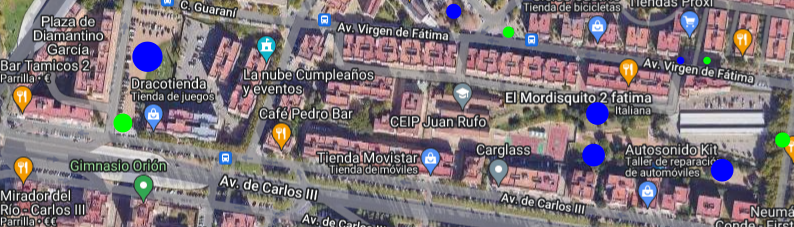
\includegraphics[width=1\linewidth]{figures/realmap}
			\label{fig:realmap}

		\end{figure}
		
		In Figure \ref{fig:blocks}, we plot the sources that are represented by green circles that simulate zones in which vans can park. The targets are also modelled by blue circles that define the zones in which customers are willing to pick up the delivery. The barriers represent buildings that drones cannot cross. To simplify the problem, we assume the drones have enough endurance to go from any source to any target and they cannot ascend to avoid the buildings and, once the number of vans is fixed, we can know the number of required drones assigned with each van.
		
		\begin{figure}[H]
			\centering
			\caption{Buildings that are presented in this part of Fátima}
			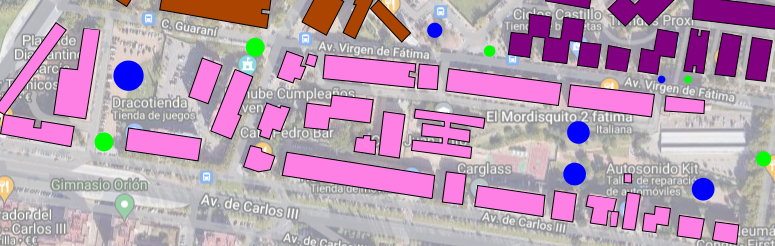
\includegraphics[width=1\linewidth]{figures/blocks}
			\label{fig:blocks}
		\end{figure}
		
		We run the single-commodity model in this scenario,  presented in Section \ref{section:formulations}, for a different number of vans $k\in\{1, 2, 3, 4\}$. It is assumed that the link distance is negligible in comparison with the Euclidean distance, i.e., $\omega_E=1$ and $\omega_L=0$. 
		
		The optimal value, measured in meters, and runtime spent to obtain the optimal solution obtained for each $k\in\{1,2,3,4\}$ are reported in Table \ref{tab:casestudy}. 
		
		% Please add the following required packages to your document preamble:
		% \usepackage{graphicx}
		\begin{table}[H]
			\centering
			\caption{Optimal solution and runtime for each configuration}
			\adjustbox{max width= \textwidth, min width = \textwidth, max height=0.05\textheight}{
			\label{tab:casestudy}%
				\begin{tabular}{ccc}
					$\bm k$ & \textbf{Optimal value} & \textbf{Runtime} \\ \hline
					\textbf{1} 	& 289.192           & 1208.53     \\
					\textbf{2} 	& 176.669           & 1417.14     \\
					\textbf{3} 	& 124.861           & 998.25      \\
					\textbf{4} 	& 110.001           & 427.47     
				\end{tabular}}%
		\end{table}
		
		The optimal solutions are represented in Figures \ref{fig:solution1}, \ref{fig:solution2}, \ref{fig:solution3} and \ref{fig:solution4}, respectively. Studying the values in Table \ref{tab:casestudy}, we can conclude that increasing the number of vans to be located reduce the total cost spent by the drones to visit all the customers at the cost of including an additional van. Although this work does not consider this ``allocation cost'', the reader may note that this issue can be dealt straightforwardly by adding an additional term in the objective function described in Section \ref{section:formulations}.
		
		
		\begin{figure}[H]
			\centering
			\caption{Solution for the case study ($k=1$)}
			\includegraphics[width=0.6\linewidth]{figures/solution1}
			\label{fig:solution1}
			\caption{Solution for the case study ($k=2$)}
			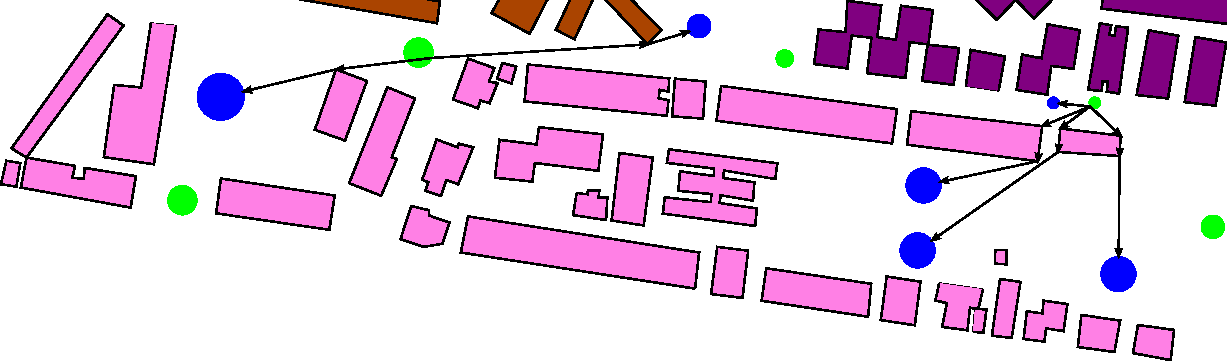
\includegraphics[width=0.6\linewidth]{figures/solution2}
			\label{fig:solution2}
			\caption{Solution for the case study ($k=3$)}
			\includegraphics[width=0.6\linewidth]{figures/solution3}
			\label{fig:solution3}
			\caption{Solution for the case study ($k=4$)}
			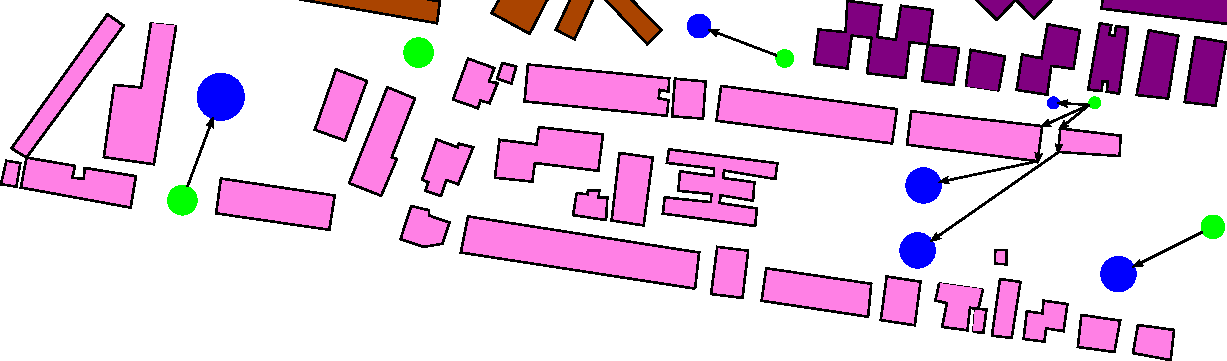
\includegraphics[width=0.6\linewidth]{figures/solution4}
			\label{fig:solution4}
		\end{figure}


		}
		
%		in this case, inspected, by the drone fleet. In addition, we assume that the drone speed is 43 km/h, while that of the helicopter is 30 km/h with the aim to minimise costs. Furthermore, we assume that the fleet consists of two drones with endurance equal to 7.5 min, and we impose that each target graph must be fully visited (inspected). As we can see in Fig. 18, Fig. 19, the origin of the mothership tour coincides with the destination and is located in an area of the city where it is possible to take off and land the helicopter. Fig. 18 reports the tour followed by the helicopter in solving the complete overlapping version of the problem, after 4 h of running time. We can observe that the helicopter, starting from the origin, flies to the point 
%		which is the first retrieval point, coinciding with the second launching point. Then it flies along the edge connecting with, that is, the second retrieval point, which coincides with the third launching point. The helicopter then flies to retrieve the drone completing the third mission. From the same point, the fourth and last mission starts and ends at the point, which is also the final destination of the helicopter tour.}
		
		
		\section{Concluding remarks}\label{section:conclusion}
		This paper has dealt with the \KMPHN \xspace and its general version called \KMPN, in which the assumption that neighbourhoods are not visible to one another is removed. \JP{The resulting problems inherit some elements from the $k$-median problem with neighbourhoods that must be exploited to partially overcome the difficulties of the solution approaches, but in addition require new techniques and algorithms  from computational geometry to handle the network design among neighbourhoods and with barriers. The \KMPN \xspace version leads to  non-convex mixed-integer problems whereas \KMPHN \xspace results in second-order cone mixed-integer problems.} The two problems, beyond its similarity, show deep differences in terms of computational difficulty, as explained in Section \ref{section:experiments}. However, the proposed mathematical programming approaches permit a formal treatment that allows one to optimally solve small to medium-size instances. For larger size instances, this approach also inspires a matheuristic algorithm providing good quality solutions, in short computing time, by exploiting the structure of the problem. It is still an open question whether there is some kind of finite dominating set with polynomial cardinality for the version \KMPHN, which certainly will simplify the underlying graph structures and the solution of the problem. Moreover, given the complexity of the problem, studying valid inequalities that reduce the space of feasible solutions will be instrumental in solving larger instances efficiently. 
		
		In addition, one can consider an extension of these problems assuming limited lengths for the paths between the source and its associated target. It would also be interesting to combine in the same model different typologies of barriers such as piecewise linear and second-order cone-representable sets. Besides, it will deserve some attention to study three-dimensional barriers that simulate buildings that planar paths cannot traverse, thus approaching even more real-life applications in the drone delivery industry. 
		
		All of the problems mentioned above are natural extensions of those considered in this paper and may attract the attention of researchers in the future.
		
		\section*{Acknowledgements}
		This research has been partially supported by the Agencia Estatal de Investigación (AEI) and the European Regional Development Fund (ERDF): PID2020-114594GB-C21; and Regional Government of Andalusia: project P18-FR-1422.
		
		
		
		
		
		
		
	
		
		
		
		
		
		
		
		
		
		
		
		
		
		
		\bibliographystyle{apa}
		\bibliography{location_barrier_bibliography.bib}
		% \printbibliography
		

	\end{document}